% !Mode::"TeX:UTF-8"
% !Mode:: "TeX:UTF-8"
\documentclass[xcolor=svgnames,serif,table,10pt]{beamer}
\mode<presentation>{
% Setup appearance:
\useoutertheme{infolines}
\usetheme{Darmstadt}
\setbeamercovered{transparent}
\setbeamertemplate{caption}[numbered]
\setbeamertemplate{navigation symbols}{}
\setbeamertemplate{blocks}[rounded][shadow=true]
\setbeamertemplate{enumerate items}[circle]

% 修改样式
\setbeamercolor{box}{bg=black!20!orange,fg=white}
\setbeamercolor{block title}{use=sidebar,fg=sidebar.fg!10!white,bg=orange!70!black}
\setbeamercolor{block title example}{use=sidebar,fg=sidebar.fg!10!white,bg=black!60!green}
\setbeamercolor{block title alerted}{use=sidebar,fg=sidebar.fg!10!white,bg=black!50!red}

\setbeamertemplate{headline}
{%
  \begin{beamercolorbox}[shadow=true]{section in head/foot}
  \vskip2pt\insertnavigation{\paperwidth}\vskip2pt
  \end{beamercolorbox}%
}
}
\usepackage{url}
\usepackage{animate}
\usepackage[english]{babel}
\usepackage{times}
\usepackage[T1]{fontenc}
\usepackage{multirow,multicol,longtable}
\usepackage{graphics}
\usepackage{xcolor}
\usepackage[no-math]{fontspec}%-------------------------------------------------- 提供字体选择命令
\usepackage{xunicode}%----------------------------------------------------------- 提供Unicode字符宏
\usepackage{xltxtra}%------------------------------------------------------------ 提供了针对XeTeX的改进并且加入了XeTeX的LOGO
\usepackage[BoldFont,SlantFont,CJKchecksingle]{xeCJK}%--------------------------- 使用xeCJK宏包


%================================== 设置中文字体 ================================%
%\setCJKmainfont{Adobe Heiti Std}%------------------------------------------------设置正文为黑体
%\setCJKmonofont{Adobe Song Std}%-------------------------------------------------设置等距字体
%\setCJKsansfont{Adobe Kaiti Std}%------------------------------------------------设置无衬线字体
% \setCJKfamilyfont{zxzt}{FZShouJinShu-S10S}
% \setCJKfamilyfont{FZDH}{FZDaHei-B02S}
%================================== 设置中文字体 ================================%

%================================== 设置英文字体 ================================%
\setmainfont[Mapping=tex-text]{Times New Roman}%--------------------------------英文衬线字体
\setsansfont[Mapping=tex-text]{Arial}%------------------------------------英文无衬线字体
\setmonofont[Mapping=tex-text]{Courier New}%-------------------------------------英文等宽字体
\newfontfamily\Arial{Arial}
%================================== 设置英文字体 ================================%

%================================== 设置数学字体 ================================%
%\setmathsfont(Digits,Latin,Greek)[Numbers={Lining,Proportional}]{Minion Pro}
%================================== 设置数学字体 ================================%
\punctstyle{kaiming}%------------------------------------------------------------ 开明式标点格式
\usepackage{graphicx}
\usepackage{tikz}
\usetikzlibrary{positioning,backgrounds}
\usetikzlibrary{fadings}
\usetikzlibrary{patterns}
\usetikzlibrary{calc}
\usetikzlibrary{shadings}
\pgfdeclarelayer{background}
\pgfdeclarelayer{foreground}
\pgfsetlayers{background,main,foreground}
\usepackage{xifthen}
\usepackage{colortbl,dcolumn}
\usepackage{enumerate}
\usepackage{pifont}
\usepackage{tabularx}
\usepackage{booktabs}
\usepackage{hyperref}

\usepackage{bm} % 字体加粗的方法
\usetikzlibrary{arrows,automata,matrix,arrows}

%=================================== 数学符号 =================================%
\newcommand{\rtn}{\mathrm{\mathbf{R}}}
\newcommand{\N}{\mathrm{\mathbf{N}}}
\newcommand{\As}{\mathrm{a.s.}}
\newcommand{\Ae}{\mathrm{a.e.}}
\newcommand*{\PR}{\mathrm{\mathbf{P}}}
\newcommand*{\EX}{\mathrm{\mathbf{E}}}
\newcommand{\EXlr}[1]{\mathrm{\mathbf{E}}\left[#1\right]}
\newcommand*{\dif}{\,\mathrm{d}}
\newcommand*{\F}{\mathcal{F}}
\newcommand*{\h}{\mathcal{H}}
\newcommand*{\vp}{\varepsilon}
\newcommand*{\prs}{\dif\PR-\As}
\newcommand*{\dte}{\dif t-\Ae}
\newcommand*{\pts}{\dif\PR\times\dif t-\Ae}
\newcommand{\Ito}{It\^{o}}
\newcommand{\tT}[1][0]{[#1,T]}
\newcommand{\intT}[2][T]{\int^{#1}_{#2}}
\newcommand{\intTe}[1][t]{\intT[t+\varepsilon]{#1}}
\newcommand{\s}{\mathcal{S}}
\newcommand{\me}{\mathrm{e}}
\newcommand{\one}[1]{{\bf 1}_{#1}}
\renewcommand{\M}{{\rm M}}
\newcommand{\Me}[1][t]{M^{\varepsilon}_{#1}}
\newcommand{\Ne}[1][t]{N^{\varepsilon}_{#1}}
\newcommand{\Pe}[1][t]{P^{\varepsilon}_{#1}}
\DeclareMathOperator*{\sgn}{sgn}
% =================================== 数学符号 =================================%

% 定义罗马数字
\makeatletter
\newcommand{\rmnum}[1]{\romannumeral #1}
\newcommand{\Rmnum}[1]{\expandafter\@slowromancap\romannumeral #1@}
\makeatother

% 定义破折号
\newcommand{\pozhehao}{\kern0.3ex\rule[0.8ex]{2em}{0.1ex}\kern0.3ex}
% 中文日期
\def\CJK@today{\the\year 年 \the\month 月}
\newcommand\zhtoday{\CJK@today}

% 中文图表
\renewcommand\figurename{图}
\renewcommand\tablename{表}

\usepackage{verbatim} % \begin{comment} xxxx \end{comment}

\graphicspath{{fig/},} 

% Author, Title, etc.

\title{信号检测与估值}

%% \subtitle{Foreground-constrained Eulerian Video Motion Magnification}

\author[段江涛]{段江涛
\\机电工程学院}

\institute[]{
\includegraphics[height=1cm]{xd.jpg}}

\date{\zhtoday}

\setlength{\baselineskip}{22pt}
\renewcommand{\baselinestretch}{1.4}

% The main document

\begin{document}
\setlength{\abovedisplayskip}{1ex}%------------------------------------------ 公式前的距离
\setlength{\belowdisplayskip}{1ex}%------------------------------------------ 公式后的距离

\begin{frame}
  \titlepage
\end{frame}

%%%%%%%%%%%%%%%%%%%%%%%%%%%%%%%% ch1
%%%%%%%%%%%%%%%%%%%%%%%%%%% ch1
\begin{frame}
  \frametitle{主要内容}
  \tableofcontents[hideallsubsections]
\end{frame}

\section{信号的随机性}
\begin{frame}
\begin{itemize}
	\item \textcolor{blue}{\textbf{信号分类}}
	\begin{itemize}
		\item[-] \textbf{确知信号}: 可以用一个确定的时间函数来表示的信号。\textcolor{red}{$s(t)(0\le t\le T)$}
		\item[-] \textbf{随机未知参量信号}:也表示为时间的函数,但信号中含有一个或一个以上的参量是随机(未知)的。\textcolor{red}{$s(t;\bm{\theta})(0\le t\le T)$}, 其中$\bm{\theta}=(\theta_1,\theta_2,\dots,\theta_M)^T$, 表示信号中含有$M$个随机(未知)参量。
	\end{itemize}
    \item \textcolor{blue}{\textbf{考虑加性噪声$n(t)$下的待处理信号(称作接收信号或观测信号)$x(t)$}}
    \begin{align*}
    \textbf{确知信号: }\qquad &x(t)=s(t)+n(t), &&(0\le t\le T)\\
    \textbf{随机(未知)参量信号: }\qquad &x(t)=s(t;\bm{\theta})+n(t), &&(0\le t\le T)
    \end{align*}
    \item \textcolor{blue}{\textbf{信号的随机性}}\\
    由于噪声$n(t)$是具有随机特性的随机过程, 即使信号是确知信号$s(t)$, 其接收信号$x(t)$也具有随机特性的信号。对于随机(未知)参量信号$s(t;\bm{\theta})$,其接收信号$x(t)$更是一随机信号。
\end{itemize}
\end{frame}

\begin{frame}
\[R=\frac{1}{2}ct_d \]
\end{frame}



% 由ch1.pptx生成pdf
%%%%%%%%%%%%%%%%%%%%%%%%%%%%%%%%%
%%%%%%%%%%%%%%%%%%%%%%%%%%% ch2-part1
\begin{frame}[shrink]
\frametitle{ch2.信号检测与估计理论的基础知识}
\framesubtitle{概率论简单回顾}
\tableofcontents[hideallsubsections]
\end{frame}


\section{样本空间,事件域,概率}

\begin{frame}{随机现象}
随机现象:\\
~\\
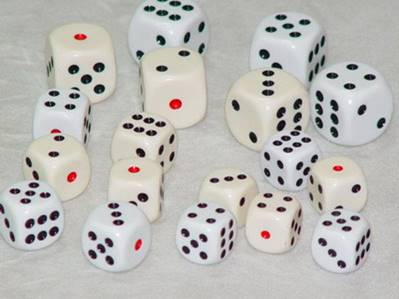
\includegraphics[scale=0.5]{die1}
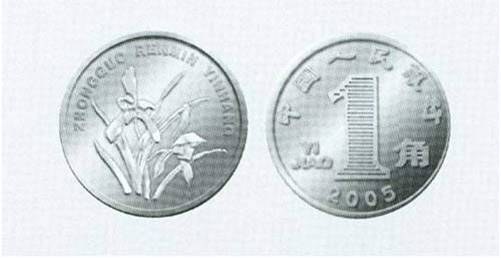
\includegraphics[scale=0.5]{coin1}\\
落叶的运动轨迹,气泡的扩散,灯泡的寿命
\begin{block}{随机现象特点}
	\begin{itemize}
		\item 至少两种可能
		\item 不确定性
	\end{itemize}
\end{block}
\end{frame}

\begin{frame}{概率论中的三个组成部分}
\begin{itemize}
	\item 样本空间$\Omega$
	\item 事件域$\mathcal{F}$
	\item 概率$P$
\end{itemize}
\end{frame}

\begin{frame}
\begin{itemize}
	\item \textbf{样本空间$\Omega$}:一个随机试验所有可能出现的结果的全体,称为随机事件的样本空间。\\
	每一个可能的结果称为基本事件,它们的全体就是样本空间。
	\item \textbf{样本点$\xi_k$}:随机试验的一个结果,就是某个基本事件,也就是$\Omega$中的一个元素。\\
	$\Omega=\{\xi_k|k=1,\dots,n\}$
	\item \textbf{随机事件$A$}: 样本空间中的某个子集称为随机事件,简称事件(事件是集合)。
    \item \textbf{事件域$\mathcal{F}$}: 样本空间中的某些子集构成的满足如下条件的集合,称为事件域(又称$\sigma^-$域)。
	\begin{itemize}
		\item[(1)] $\Omega\in\mathcal{F}$
		\item[(2)] 若$A\in\mathcal{F}$, 则$A$的补$\overline{A}\in\mathcal{F}$
		\item[(3)] 若$A_n\in\mathcal{F}, n=1,2,\dots$, 则$\bigcap\limits_{n=1}^{\infty}A_n\in\mathcal{F}$
	\end{itemize}
\end{itemize}
\end{frame}

\begin{frame}
\begin{example}
	一个盒子中有10个相同的球,5个 白色,5个黑色,搅匀后从中任意摸取一球。\\
	~\\
	样本点: $\xi_1=\{\text{取得白球} \}$, $\xi_2=\{\text{取得黑球} \}$\\
	样本空间: $\Omega=\{\xi_1,\xi_2\}$
\end{example}
\begin{example}
	一个盒子中有10个相同的球,编号1,2,...,10, 从中取一球。\\
	样本空间: $\Omega=\{1,2,\dots,10\}$\\
	随机事件: $A=\{\text{6号球} \}=\{6\}$, $B=\{\text{偶数编号球} \}=\{2,4,6,8,10\}$, $\overline{B}=\{\text{奇数编号球}\}$,$C=\{\text{编号小于等于5的球} \}=\{1,2,3,4,5\}$\\
	事件A是基本事件,而B和C则由多个基本事件所组成,并且$A,B,C\subset\Omega$。
\end{example}
\textit{空集$\emptyset$可以看作$\Omega$的子集,在任意一次试验中不可能有此事件发生,称为不可能事件。}
\end{frame}

\begin{frame}{事件$A$的概率$P(A)$}
  事件域中的元素就是随机事件。如果这些事件的随机性能够由定义在事件域$\mathcal{F}$上的具有非负性,归一性和可列加性的实函数$P(A)$来确定,则称$P$是定义在二元组$(\Omega,\mathcal{F})$上的概率,而称$P(A)$为事件$A$的概率。
  \begin{enumerate}
  	\item[(1)] 非负性。 $P(A)\ge 0$
  	\item[(2)] 归一性。 $P(\Omega)=1$
    \item[(3)] 可列加性。$A_1,A_2,...,A_n$互不相容$(A_i\cap A_j=\emptyset,i\ne j)$,则$P(A_1\cup A_2\cup\dots\cup A_n) = P(A_1)+P(A_2)+\cdots+P(A_n)$
  \end{enumerate}
\end{frame}

\begin{frame}
\frametitle{等可能概型(古典概型)}
\begin{itemize}
	\item 样本空间的元素(即基本事件)只有有限个,不妨设为$n$个,$\Omega=\{\xi_1,\xi_2,\dots,\xi_n\}$
	\item 每个基本事件出现的可能性是相等的,即有$P(\xi_1)=P(\xi_2)=\cdots=P(\xi_n)$
	\item 事件域$\mathcal{F}$为$\Omega$的所有子集的全体,即是$Pwr(\Omega),\Omega$的幂集,共有$2^n$个事件,$\emptyset\in\mathcal{F},\Omega\in\mathcal{F}$。
	\item 由概率的有限可加性知\\
	$1=P(\Omega)=\sum\limits_{i=1}^{n}P(\xi_i)\implies P(\xi_i)=\frac{1}{n},(i=1,\dots,n)$
	\item 对任意一个随机事件$A\subseteq\mathcal{F}$, 如果$A$是$k$个基本事件的和,即$A=\{\xi_{i_1}\}\cup \{\xi_{i_2}\}\cup\cdots\cup\{\xi_{i_k}\}$, 则
	$$P(A)=\frac{k}{n}=\frac{\text{$A$中所包含的基本事件数}}{\text{基本事件总数}}$$
\end{itemize}
\end{frame}

\begin{frame}
\begin{example}
	将一枚硬币抛掷3次,(1) 设事件$A_1$为``恰有一次出现正面'', 求$P(A_1)$;
	(2) 设事件$A_2$为``至少一次出现正面'',求$P(A_2)$。
	\begin{enumerate}
		\item 正面用$H$表示, 反面用$T$表示。则\\
		样本空间$\Omega=\{HHH,HHT,HTH,HTT,THH,THT,TTH,TTT\}$\\
		事件$A_1=\{HTT,THT,TTH\}$。\\
		$\Omega$中包含有限个元素, 且由对称性知, 每个基本事件发生的可能性相同。所以, $P(A_1)=\frac{3}{8}$。
		\item 由于$\overline{A_2}=\{TTT\}$, 于是\\
		$P(A_2)=1-P(\overline{A_2})=1-\frac{1}{8}=\frac{7}{8}$
	\end{enumerate}
\end{example}
\end{frame}

\begin{frame}
\frametitle{样本空间的选取}
为求一个事件的概率,样本空间可以有不同的取法,但一定要保证基本事件和求概事件数的计算都要在\textbf{同一个样本空间}中进行,否则会导致谬误!
\begin{example}
	一个盒子中有10个相同的球,编号1,2,...,10, 从中取一球,求此球的号码为偶数的概率。\\
	样本空间$\Omega=\{1,2,\dots,10\}$\\
	事件$A=\{\text{偶数编号球} \}=\{2\}\cup\{4\}\cup\{6\}\cup\{8\}\cup\{10\}=\{2,4,6,8,10\}$。\\
	$P(A)=\frac{|A|}{n}=\frac{5}{10}=\frac{1}{2}$
\end{example}
另外一种解法:$\Omega=\{A,\overline{A}\},A=\{\text{编号为偶数的球}\},\overline{A}=\{\text{编号为奇数的球}\},\mathcal{F}=\{\emptyset,\Omega,A,\overline{A}\}$,由$A,\overline{A}$的对称性,即得$P(A)=\frac{1}{2}$

\end{frame}

\begin{frame}
\frametitle{样本空间的选取}
\begin{block}{Notes}
	\begin{itemize}
		\item 两种解法的样本空间$\Omega$不同(从而事件域$\mathcal{F}$是不同的)。
		\begin{enumerate}
			\item $\Omega=\{1,2,\dots,10\}$ 
			\item $\Omega=\{A,\overline{A}\}$
		\end{enumerate}
	   \item 严格地说,两者所描述的随机试验是不同的。\\
	   例如对于第二种解法来说,$B=\{\text{号码为4的球}\}$并不属于事件域$\mathcal{F}$,就是说$B$不是一个事件,从而也就没有概率可言。\\
	   但对第一种解法,$B$是事件,而且$P(B)=\frac{1}{10}$。
	   \item 一定要保证基本事件和求概事件数的计算都要在\textbf{同一个样本空间}中进行。
	\end{itemize}
\end{block}
\end{frame}

\section{条件概率,全概率公式}

\begin{frame}{条件概率}
\begin{definition}
	若$\Omega,\mathcal{F},P$是一个概率空间,$B\in\mathcal{F}$, 且$P(B)>0$,则对任意的$A\in\mathcal{F}$,称
	$$P(A|B)=\frac{P(AB)}{P(B)}$$
	为在已知事件B发生的条件下,事件A发生的条件概率。
\end{definition}

\begin{columns}%0.6 0.4表示相对比例
	\column{0.4\textwidth}%<1->
\[P(A|B)=\frac{S_{AB}}{S_B}=\frac{S_{AB}/S_\omega}{S_B/S_\omega}=\frac{P(AB)}{P(B)} \]
	\column{0.4\textwidth}%<1->
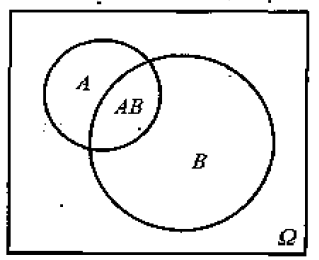
\includegraphics[scale=0.2]{P(AB)}
\end{columns}
\end{frame}

\begin{frame}{条件概率的性质及其推论}
\begin{block}{条件概率$P(\bullet|B)$的具备概率的三个基本性质}
	\begin{enumerate}
		\item 非负性: 对任意的$A\in F, P(A|B)\ge 0$;
		\item 规范性: $P(\Omega|B)=1$;
		\item 可列加性: 对任意的一列两两互不相容的事件$A_i(i=1,2,\dots)$, 有
		\[P\left[\bigcup\limits_{i=1}^{+\infty}(A_i|B)\right]=\sum\limits_{i=1}^{+\infty}P(A_i|B) \]
	\end{enumerate}
\end{block}
\begin{corollary}
概率的乘法公式:  $P(AB)=P(B)P(A|B)$
\end{corollary}

\begin{corollary}
	$P(A_1A_2\cdots A_n)=P(A_1)P(A_2|A_1)P(A_3|A_1A_2)\cdots P(A_n|A_1A_2\cdots A_{n-1})$
\end{corollary}
\end{frame}

\begin{frame}
\begin{example}
	一个家庭中有两个小孩,已知其中有一个是女孩,问这时另一个小孩也是女孩的概率有多大?
	
	\medskip
	$\Omega=$\{(男,男),(男,女),(女,男),(女,女)\}\\
	$A=$\{已知有一个是女孩\}=\{(男,女),(女,男),(女,女)\}\\
	$B=$\{另一个也是女孩\}=\{(女,女)\}\\
	于是所求概率为\\
	$P(B|A)=\frac{P(AB)}{P(A)}=\frac{1/4}{3/4}=\frac{1}{3}$
\end{example}
\end{frame}

\begin{frame}{概率树/全概率公式}
概率树思想:为了求解复杂事件的概率,往往可以先把它分解成两个(或若干个)互不相容的较简单的事件之并。求出这些较简单事件的概率,再利用加法公式即得所要求的复杂事件的概率。把这个方法一般化,便的到下述定理。
\begin{theorem}
	设$B_1,B_2,\cdots$是一列互不相容的事件,且有
	\[\bigcup_{i=1}^{+\infty}B_i=\Omega,P(B_i)>0 \]
	则对任一事件A,有
	\[P(A)=\sum_{i=1}^{+\infty}P(B_i)P(A|B_i) \]	
\end{theorem}
\end{frame}

\begin{frame}
\begin{example}
	某工厂有4条流水线生产同一种产品, 该4条流水线的产品分别占总产量的15\%, 20\%, 30\%, 35\%, 又这4条流水线的不合格品率依次为0.05, 0.04, 0.03及0.02. 现从出厂产品中任取一件, 问
	\begin{enumerate}
		\item 恰好抽到不合格品的概率为多少? 
		\item 第4条流水线应承担的责任?
	\end{enumerate} 
\end{example}
\end{frame}

\begin{frame}[shrink]
解: (1) 令
\begin{align*}
A&=\{\text{任取一件,恰好抽到不合格品} \}\\
B&=\{\text{任取一件,恰好抽到第$i$条流水线的产品}, (i=1,2,3,4) \}
\end{align*}
于是由全概率公式可得
\begin{align*}
P(A)&=\sum\limits_{i=1}^4P(B_i)P(A|B_i)=0.15\times 0.05+0.20\times 0.04+0.30\times 0.03+0.35\times 0.02\\
&=0.0315=3.15\%
\end{align*}
实际上,$P(A|B_i)$可以从过去生产的产品中统计出来,称为\textbf{先验概率}。\\
(2) 从概率论的角度考虑可以按$P(A|B_i)$的大小来追究第$i$条$i=1,2,3,4$流水线的责任。\\
$P(AB_4)=P(B_4)P(A|B_4)=0.35\times 0.02=0.007$\\
由条件概率的定义知
\begin{align*}
P(B_4|A)=\frac{P(AB_4)}{P(A)}=\frac{P(B_4)P(A|B_4)}{\sum\limits_{i=1}^4P(B_i)P(A|B_i)}=\frac{0.007}{0.0315}\approx 0.222
\end{align*}
\end{frame}

\begin{frame}{相互独立事件}
条件概率: $P(B|A)=\frac{P(AB)}{P(A)}$\\
一般的概率乘法公式: $P(AB)=P(A)P(B|A)$\\
如果``事件B发生与否不受事件A的影响'': $P(B)=P(B|A)$\\
乘法公式变为: $P(AB)=P(A)P(B)$
\begin{definition}
对任意的两个事件A,B,若
\[P(AB)=P(A)P(B)\]
成立,则称事件A,B是相互独立的,简称为独立的。	
\end{definition}
\begin{block}{依这个定义,不难验证:}
	若A与B相互独立,则$\{\emptyset,A,\overline{A},\Omega\}$中的任意一个与$\{\emptyset,B,\overline{B},\Omega\}$中的任意一个仍相互独立。
\end{block}
\end{frame}

\begin{frame}[shrink]
		分别掷两枚均匀的硬币,令
		\begin{align*}
		A=\{\text{硬币甲出现正面} \}\quad	B=\{\text{硬币乙出现正面} \}
		\end{align*}
		验证事件$A,B$是相互独立的。
 \begin{proof}
			$$\text{样本空间}=\{\text{(正,正),(正,反),(反,正),(反,反)}\} $$
			共还有4个基本事件,它们是等可能的,各有概率为1/4,而
			\begin{align*}
			A&=\{\text{(正,正),(正, 反)}\} \\
			B&=\{\text{(正,正),(反, 正)}\} \\
			AB&=\{\text{正,正}\}
			\end{align*}
			由此知 \[P(A)=P(B)=\frac{1}{2}\]
			这时有 \[P(AB)=\frac{1}{4}=P(A)P(B)\]
			成立,所以A, B事件是相互独立的。
 \end{proof}
\end{frame}

\section{随机变量}

\begin{frame}
\begin{definition}
	设$(\Omega,\mathcal{F},P)$是一概率空间,$X=X(\xi),\xi\in\Omega$是定义在$\Omega$上的单值实函数,如果对任一实数$x$, 集合$\{\xi|X(\xi)\le x\}\in\mathcal{F}$ 则称$X=X(\xi)$为$(\Omega,\mathcal{F},P)$上的一个\textbf{随机变量}。
	
	随机变量$X(\xi)$的定义域为样本空间$\Omega$,它的值域是实数R。所以,随机变量$X(\xi)$实际上是一个映射,这个映射为每个来自概率空间的结果(样本点)$\xi$赋予一个实数$x$。这种映射必须满足条件:
	\begin{itemize}
		\item[(1)] 对任一$x$,集合$\{\xi|X(\xi)\le x\}\in\mathcal{F}$(即,使得$X(\xi)\le x$的所有样本点$\xi$所组成的集合)是这个概率空间中的一个事件,并有确定的概率$P\{X(\xi)\le x\}$;
		\item[(2)] $P\{X(\xi)=\infty \}=0$, $P\{X(\xi)=-\infty \}=0$
	\end{itemize}
\end{definition}
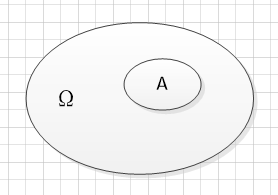
\includegraphics[scale=0.2]{geometry}
\end{frame}

\begin{frame}
\begin{example}
	将一枚硬币抛掷3次,正面用$H$表示, 反面用$T$表示, 则样本空间
	\[\Omega=\{HHH,HHT,HTH,HTT,THH,THT,TTH,TTT\} \]
	令随机变量$X(\xi)$表示投掷得到正面的总数。则
	\[ 
		X=X(\xi)=
		\begin{cases}
		3, &\xi=\{HHH\}\\
		2, &\xi=\{HHT,HTH,THH\}\\
		1, &\xi=\{HTT,THT,TTH\}\\
		0, &\xi=\{TTT\}
		\end{cases}
	\]
	$X=2$, 对应样本点的集合$A=\{HHT,HTH,THH\}$,是一个事件, 其概率$P\{X=2\}=P(A)=3/8$。类似地有
	\[ P\{X\le 1\}=P\{\{X=0\}\cup\{X=1\}\}=P\{HTT,THT,TTH,TTT\}=\frac{1}{2} \]
\end{example}
\end{frame}

\begin{frame}
随机变量的取值随试验的结果而定, 而试验的各个结果出现有一定的概率, 因而随机变量的取值有一定的概率。
\begin{definition}
	设$X=X(\xi)$是随机变量, 若$L$是一个实数集合, $L\subseteq\mathbb{R}, $将$X$在$L$上取值写成$\{X\in L\}$. 它表示事件$B=\{\xi|X(\xi)\in L \}$. 即$B$是由$\Omega$中使得$X(\xi)\in L$的所有样本点$\{\xi\}$所组成的事件, 此时有
    \[P\{X\in L\}=P(B)=P\{\xi|X(\xi)\in L\} \]
\end{definition}
\begin{block}{Notes}
	随机变量$X=X(\xi)$就是试验结果(即样本点)和实数之间的一一对应关系。虽然在试验之前不能肯定随机变量$X=X(\xi)$会取哪一个数值,但是对于任一实数$a$, 我们可以研究$\{X=X(\xi)=a \}$发生的概率, 也就是$X(\xi)$取值的统计规律。
\end{block}
\end{frame}

\begin{frame}{随机变量的分布函数}
\begin{definition}
	设$X$是随机变量, 对$\forall x\in\mathbb{R}$, 称函数
	\[F(x)=P\{X\le x\}, -\infty<x<\infty\]
	为随机变量$X$的一维(累积)分布函数[(cumulative) distribution function]。
\end{definition}
对于任意实数$x_1,x_2(x_1<x_2)$,有
\[P\{x_1<X\le x_2\}=P\{X\le x_2\}-P\{X\le x_1\}=F(x_2)-F(x_1) \]
\begin{block}{Notes}
	如果将$X$看成是数轴上的随机点的坐标, 那么, 分布函数$F(x)$在$x$处的函数值就表示$X$落在区间$(-\infty,x]$上的概率。
\end{block}
\end{frame}

\begin{frame}
\begin{block}{分布函数性质}
	\begin{enumerate}
		\item 单调不减性: 对$\forall x_1<x_2$, 恒有$F(x_1)\le F(x_2)$\\
		对于任意实数$x_1,x_2(x_1<x_2)$,有
		\[F(x_2)-F(x_1)=P\{x_1<X\le x_2\}\ge 0 \]
		\item 规范性: $0\le F(x)\le 1$, 且
		\[ F(-\infty)=\lim\limits_{x\to -\infty}F(x)=0,\quad F(+\infty)=\lim\limits_{x\to +\infty}F(x)=1 \]
		\item 右连续性: 对$\forall x_0$, 恒有$F(x_0+0)=\lim\limits_{x\to x_0^+}F(x)=F(x_0)$
	\end{enumerate}
\end{block}
\begin{block}{几何说明}
	将$X\in [0,x]$的端点$x$沿数轴无限向左移动(即$x\to -\infty$), 则``随机点$X$落在点$x$左边''这一事件趋于不可能事件, 从而概率趋于$0$, 即有$F(-\infty)=0$;
	
	\medskip
	将$X\in [0,x]$的端点$x$沿数轴无限向右移动(即$x\to \infty$), 则``随机点$X$落在点$x$左边''这一事件趋于必然事件, 从而概率趋于$1$, 即有$F(\infty)=1$;
\end{block}

\end{frame}

\begin{frame}{随机变量的概率密度函数$p(x)$}
\begin{definition}
	设连续随机变量$X$的\textbf{一维累积分布函数}为$F(x)$, 如果$F(x)$对$x$的一阶导数存在,则有
	\[p(x)\mathop{=}^{def}\frac{dF(x)}{dx}\]
	式中, $p(x)$称为随机变量$X=X(\xi)$的\textbf{一维概率密度函数}, 简称概率密度函数(probability density function, p.d.f)
\end{definition}
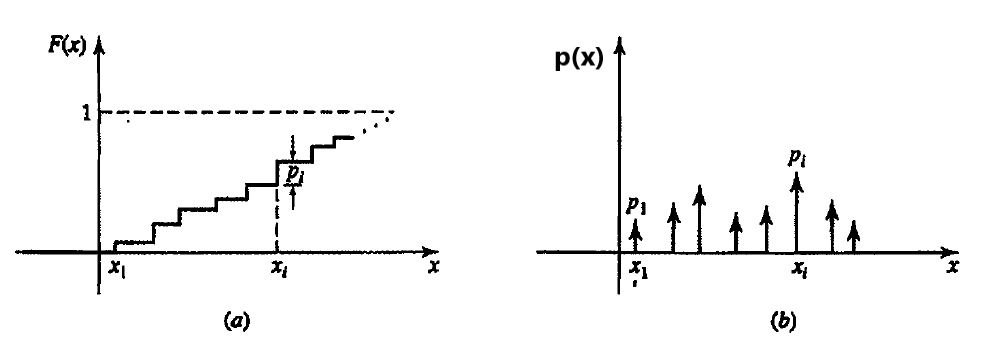
\includegraphics[scale=0.4]{pi}
\end{frame}

\begin{frame}[shrink]
\frametitle{随机变量概率密度函数$p(x)$的性质}
\begin{enumerate}
	\item 根据随机变量$x(\xi)$的$p(x)$与$F(x)$的关系, 有
	\[F(x)=\int_{-\infty}^{x}p(u)du\]
	\item 对所有$x$, p(x)是非负函数,即
	\[p(x)\ge 0,\quad -\infty<x<+\infty \]
	\item $p(x)$对$x$的全域积分结果等于1, 一般表示为
	\[\int_{-\infty}^{\infty}p(x)dx=1\]
	\item 随机变量$x(\xi)$落在区间$[x_1,x_2]$内的概率为
	\[P\{x_1\le x(\xi)\le x_2\}=F(x_2)-F(x_1)=\int_{x_1}^{x_2}p(x)dx\]
\end{enumerate}
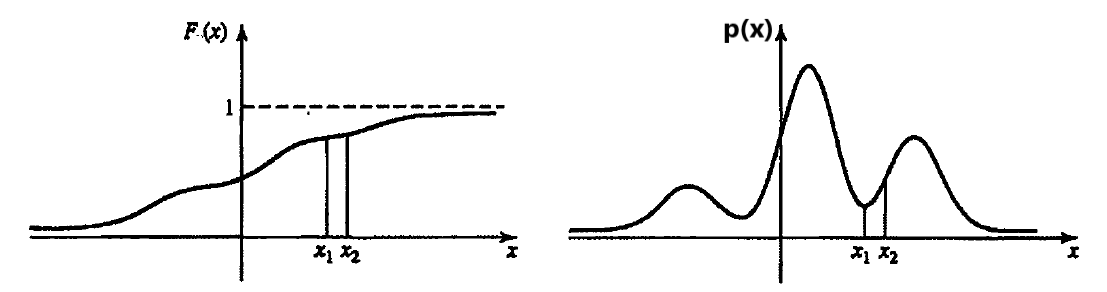
\includegraphics[scale=0.3]{Fx-px2}
\end{frame}

\section{离散型随机变量及其分布律}

\begin{frame}[shrink]
%\frametitle{离散型随机变量}
\begin{definition}[离散型随机变量]
	定义在样本空间$\Omega$上,取值于实数域$\mathbb{R}$,且只取\textcolor{blue}{有限个或可列个值}的变量$X=X(\xi)$, 称作是\textbf{一维(实值)离散型随机变量}。\\
\end{definition}

\begin{definition}[离散型随机变量的概率]
	设离散型随机变量$X$所有可能取的值为$x_k(k=1,2,\dots)$, $X$取各个可能值的概率, 即事件$\{X=x_k\}$的概率为
	\[P\{X=x_k\}=p_k, k=1,2,\dots\]
\end{definition}

由概率的定义, $p_k$满足如下两个条件: 
\begin{enumerate}
	\item $p_k\ge 0, k=1,2,\dots$
	\item $\sum\limits_{k=1}^{\infty}p_k=1$\\
	因为$\{X=x_1\}\cup\{X=x_2\}\cup\cdots$是必然事件, 且$\{X=x_j\}\cap\{X=x_k\}=\emptyset, k\ne j$故
	\[1=P[\bigcup_{k=1}^{\infty}\{X=x_k\}]=\sum_{k=1}^{\infty}P\{X=x_k\}=1 \]
\end{enumerate}
\end{frame}

\begin{frame}{离散型随机变量$X$的分布律}
离散型随机变量$X$的分布律的解析表达式:
	\[P\{X=x_k\}=p_k, k=1,2,\dots\]
可用表格形式表示如下:
\begin{block}{离散型随机变量$X$的分布律}
	%\begin{tabular}{c|c|c|c|c|c|}
	\begin{tabular}{c|ccccc}
		%\hline 
		$X$ & $x_1$ & $x_2$ & $\cdots$ & $x_n$ & $\cdots$\\ 
		\hline 
		$p_k$ & $p_1$ & $p_2$ & $\cdots$ & $p_n$ & $\cdots$\\ 
		%\hline 
	\end{tabular} 
\end{block}

\begin{example}
	某产品40件,其中次品3件,现从中任取3件。(1) 求取出的3件产品中所含次品数$X$的分布律; (2) 求取出的产品中至少有一件次品的概率; (3) 求离散型随机变量$X$的分布函数$F(x)$。
\end{example}
\end{frame}

\begin{frame}
\begin{block}{解:}
(1) \begin{tabular}{ll}
	$P\{X=0\}=\frac{C_{37}^{3}}{C_{40}^{3}}=0.7865$ & $P\{X=1\}=\frac{C_{3}^{1}C_{37}^{2}}{C_{40}^{3}}=0.2022$ \\ 
	$P\{X=2\}=\frac{C_{3}^{2}C_{37}^{1}}{C_{40}^{3}}=0.0112$ & $P\{X=3\}=\frac{C_{3}^{3}}{C_{40}^{3}}=0.0001$ \\ 
\end{tabular}\\ 
(2) \quad $P\{X\ge 1\}=1-P\{X=0\}=1-0.7865=0.2135$\\
(3) 由分布函数定义得:
$F(x)=P\{X\le x\} =
\begin{cases}
0,      & x<0 \\
0.7865, & 0\le x<1 \\
0.9887, & 1\le x<2 \\
0.9999, & 2\le x<3 \\
1,      & x\ge 3
\end{cases} $
\end{block}
\begin{columns}%0.6 0.4表示相对比例
	\column{0.4\textwidth}%<1->
	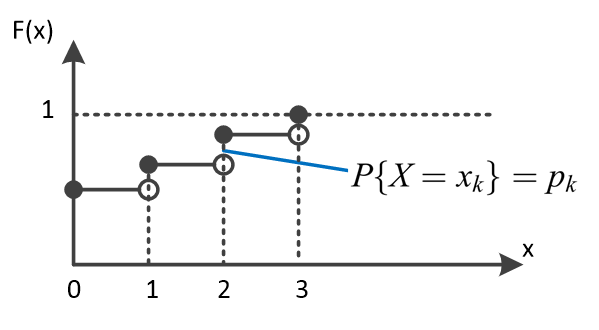
\includegraphics[scale=0.22]{fx}
	\column{0.6\textwidth}%<1->
	由$F(x)$的图示看到, $F(x)$是一个阶梯状的右连续函数($F(x+0)=F(x)$),在$x=k$处有跳跃,跃度为在$X=k$处的概率$p_k=P\{X=k\}$。	
\end{columns}
\end{frame}

\begin{frame}
\begin{columns}
\column{0.4\textwidth}
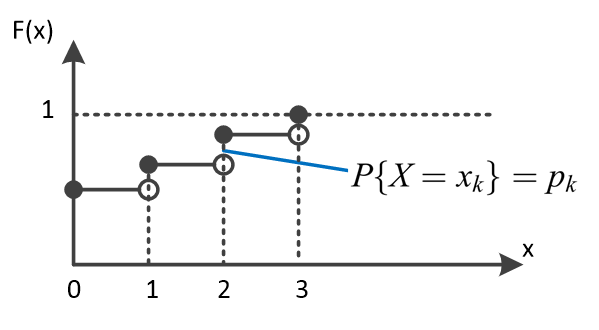
\includegraphics[scale=0.22]{fx}
\column{0.6\textwidth}
由随机变量$X$的分布函数$F(x)$, 可以计算
\begin{block}{}
\begin{align*}
P(X \le x) &= F(x)\\
P(X = x) &= F(x)-F(x-0) \\
P(X < x) &= F(x-0) \\
P(X > x) &= 1- F(x) \\
P(X \ge x) &= 1-F(x-0)
\end{align*}
进一步,形如$\{x_1\le X\le x_2\},\{x_1< X< x_2\},\{x_1< X\le x_2\}, \{x_1\le X< x_2\}$等一些事件及它们经过有限次或可列次并、交、差运算以后的概率,都可以由$F(x)$计算出来。
\end{block}
\end{columns}
\begin{block}{}
\textcolor{blue}{$F(x)$全面地描述了随机变量$X$的统计规律。}
\end{block}
\end{frame}

\section{狄拉克函数(Dirac函数/$\delta$函数)}

\begin{frame}{狄拉克函数(Dirac函数/$\delta$---函数)}
\begin{definition}[$\delta$---函数]
	对于任意的无穷次可微的函数$f(t)$, 如果满足:
	$$\int_{-\infty}^{\infty}\delta (t)f(t)dt=\lim\limits_{\varepsilon\to 0}\int_{-\infty}^{\infty}\delta_{\varepsilon}(t)f(t)dt $$
	其中:
	\[
	\delta_{\varepsilon}(t)=\begin{cases}
	0,&t<0\\
	\frac{1}{\varepsilon}, & 0\ge t<\varepsilon\\
	0, &t>\varepsilon
	\end{cases}
	\]
	则称$\delta_\varepsilon(t)$的弱极限为$\delta$函数,记为$\delta(t)$
	显然, 对于任意的$\varepsilon>0$, 有:
	$$\int_{-\infty}^{\infty}\delta_{\varepsilon}(t)dt=\int_{-\infty}^\infty\frac{1}{\varepsilon}dt=1\implies \int_{-\infty}^\infty\delta(t)dt=1$$
\end{definition}
\end{frame}

\begin{frame}{狄拉克函数(Dirac函数/$\delta$---函数)}
\begin{block}{注}
\begin{enumerate}
	\item $\delta(t)$在$t=0$点的取值为$\infty$, 在$t\ne 0$点的取值为0, 并且满足$\int_{-\infty}^{\infty}\delta(t)dt=1$。
	\item 工程(信号处理等)上$\delta$---函数也称为单位脉冲或单位冲激函数。
\end{enumerate}
\end{block}
\begin{block}{$\delta$---函数的筛选性质}
若$f(t)$为无穷此可微的函数,则有:$\int_{I}\delta(t)f(t)dt=f(0) $\\
其中$I$是包含点$t=0$的任意区间。特殊地, 有:$\int_{-\infty}^{\infty}\delta(t)f(t)dt=f(0) $\\
更一般地,我们有:
$$\int_{-\infty}^{\infty}\delta(t-t_0)f(t)dt=f(t_0) $$
\end{block}
\end{frame}

\begin{frame}[shrink]
\frametitle{离散型随机变量分布律的$\delta$---函数表示}
设离散型随机变量$X$的分布律为: $P\{X=x_i\}=p_i,i=1,2,\dots$, 则由$\delta$---函数的筛选性质可以定义离散型随机变量$X$的概率密度函数为:
$$p(x)=\sum\limits_{i=0}^{\infty}p_i\delta(x-x_i)$$
因为,由$\delta$---函数的筛选性质,离散型随机变量$X$的分布函数可以表示为:
$$F(x)=P\{X\le x\}=\sum\limits_{x_i\le x}p_i=\int_{-\infty}^{x}\sum\limits_{i=1}^{\infty}p_i\delta(u-x_i)du$$
\[P\{X=x_i\}=F(x_i)-F(x_i^{-})=p_i\]
\begin{columns}
	\column{0.4\textwidth}
	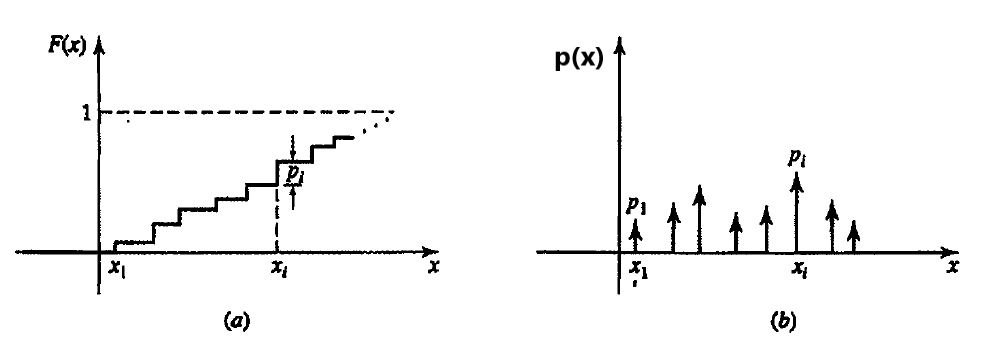
\includegraphics[scale=0.2]{pi}
	\column{0.4\textwidth}
	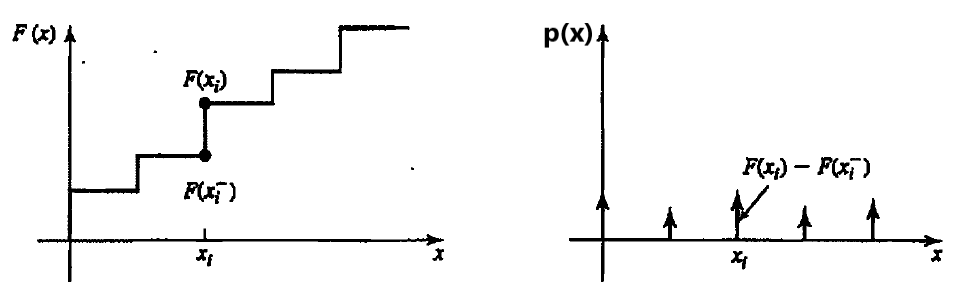
\includegraphics[scale=0.2]{Fx-px}
\end{columns}
\end{frame}

\begin{frame}[shrink]
\frametitle{离散型随机变量与连续性随机变量的统一}
\begin{block}{}
	工程上,常用离散型随机变量分布律的$\delta$---函数表示法,将离散型随机变量的分布律表示成概率密度函数的形式,因此与连续型随机变量的概率密度函数$p(x)$一样进行统一处理。
\end{block}
$$P\{x_1\le X\le x_2\}=\int_{x_1}^{x_2}p(x)dx$$
离散型随机变量:
	$$F(x)=P\{X\le x\}=\sum\limits_{x_i\le x}p_i=\int_{-\infty}^{x}\sum\limits_{i=1}^{\infty}p_i\delta(u-x_i)du$$
	$$p(x)=\sum\limits_{i=0}^{\infty}p_i\delta(x-x_i)$$
连续型随机变量:
	$$p(x)\mathop{=}^{def}\frac{dF(x)}{dx},\quad F(x)=P\{X\le x\}=\int_{-\infty}^{x}p(u)du$$

\end{frame}

\begin{frame}[shrink]
\begin{example}
抛掷一枚硬币: 样本空间: $\Omega=\{H,T\}$, $H$表示正面, $T$表示反面。正面的概率$p$, 反面的概率$q$. 定义随机变量$X=X(\xi),\xi\in \Omega$满足:
	\[X(\xi=H)=1\qquad X(\xi=T)=0,\]
	求分布函数$F(x)$和概率密度函数$p(x)$,其中: $-\infty<x<\infty$.
\end{example}
\begin{align*}
&P\{X=0\}=q,\quad P\{X=1\}=p\\
&F(x)=P\{X\le x\}=\sum\limits_{x_i\le x}p_i=\int_{-\infty}^{x}\sum\limits_{i=1}^{\infty}p_i\delta(u-x_i)du\\
&p(x)=\sum\limits_{i=0}^{\infty}p_i\delta(x-x_i)
\end{align*}
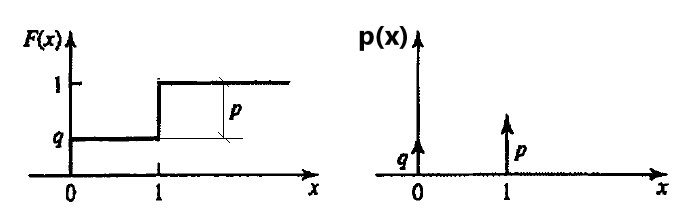
\includegraphics[scale=0.4]{coin-tossing} 
X\end{frame}

\begin{frame}[shrink]
\begin{example}
事件A, 试验的样本空间: $\Omega=\{A,\overline{A},\emptyset \}$. 定义随机变量$X=X(\xi)$,
满足:
\begin{align*}
	X(\xi)=1, &\quad \xi\in A\\
	X(\xi)=0, &\quad \xi\in\overline{A}
\end{align*}
\end{example}
\begin{align*}
&P\{X=1\}=P(A)=p,\quad P\{X=0\}=P(\overline{A})=q=1-p\\
&F(x)=P\{X\le x\}=\sum\limits_{x_i\le x}p_i=\int_{-\infty}^{x}\sum\limits_{i=1}^{\infty}p_i\delta(u-x_i)du\\
&p(x)=\sum\limits_{i=0}^{\infty}p_i\delta(x-x_i)
\end{align*}
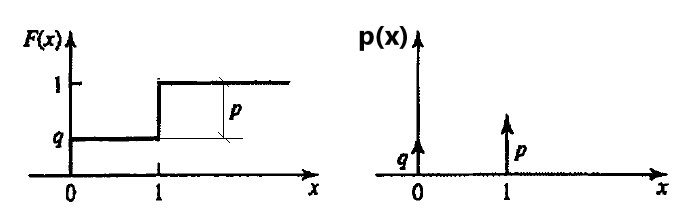
\includegraphics[scale=0.4]{coin-tossing}
\end{frame}

\begin{frame}[shrink]
\begin{example}
抛掷两枚硬币: 随机变量$X=X(\xi)$表示正面数目。\\
样本空间: $\Omega=\{HH,HT,TH,TT\}$, $H$表示正面, $T$表示反面。\\
随机变量$X(HH)=2,\quad X(HT)=1, \quad X(TH)=1, \quad X(TT)=0$ \\
求$F(x)$和$p(x)$.
\end{example}
\begin{align*}
&P\{X=0\}=\frac{1}{4}, \quad P\{X=1\}=\frac{2}{4},\quad P\{X=2\}=\frac{1}{4}\\
&F(x)=P\{X\le x\}=\sum\limits_{x_i\le x}p_i=\int_{-\infty}^{x}\sum\limits_{i=1}^{\infty}p_i\delta(u-x_i)du\\
&p(x)=\sum\limits_{i=0}^{\infty}p_i\delta(x-x_i)
\end{align*}
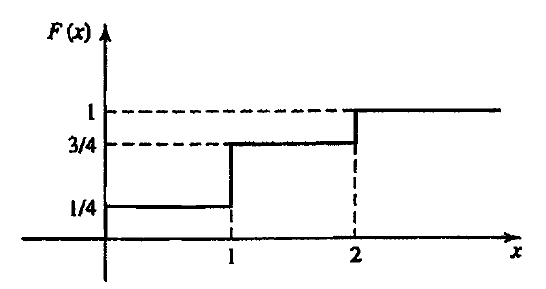
\includegraphics[scale=0.3]{coin-tossing2} \medspace \medspace
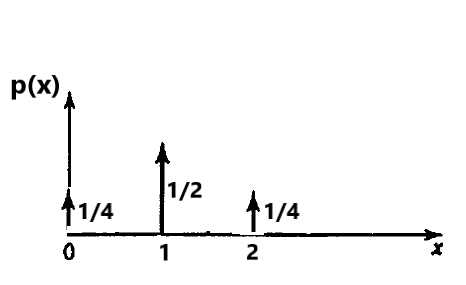
\includegraphics[scale=0.3]{coin-tossing22}
\end{frame}

\begin{frame}[shrink]
掷一枚骰子: 样本空间: $\Omega=\{f_1,f_2,f_3,f_4,f_5,f_6\}$。定义随机变量$X=X(\xi),\xi\in \Omega$满足:$X(f_i)=10i$
求$F(x)$和$p(x)$,其中: $-\infty<x<\infty$.\\
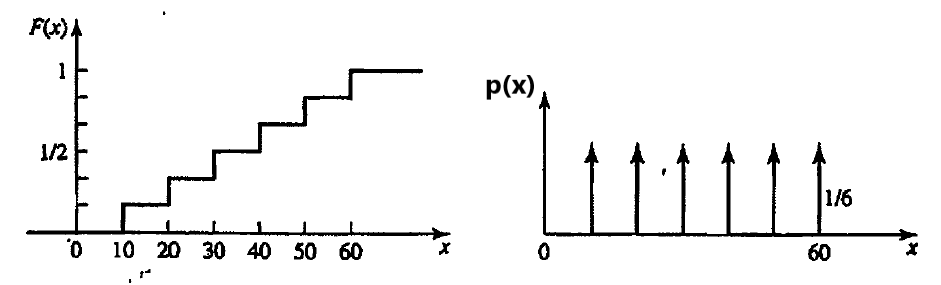
\includegraphics[scale=0.4]{die}
\begin{align*}
F(100)&=P\{X(\xi)\ge 60 \}=P(\Omega)=1\\
F(35)&=P\{X(\xi)\le 35 \}=P\{f_1,f_2,f_3 \}=\frac{3}{6} \\
F(30.01)&=P\{X(\xi)\le 30.01 \}=P\{f_1,f_2,f_3 \}=\frac{3}{6} \\
F(30)&=P\{X(\xi)\le 30 \}=P\{f_1,f_2,f_3 \}=\frac{3}{6} \\
F(29.9)&=P\{X(\xi)\le 29.9 \}=P\{f_1,f_2 \}=\frac{2}{6} \\
\end{align*}
\end{frame}



 %概率论简单回顾
%%%%%%%%%%%%%%%%%%%%%%%%%%% ch2
\begin{frame}
  \frametitle{主要内容}
  \tableofcontents[hideallsubsections]
\end{frame}

\section{随机变量}

\begin{frame}
随机事件的特征是不确定性,但是我们可以通过重复观测,从不确定现象中寻找、观察特定事件发生的规律,为此需要让某一随机现象重复发生(不一定是人为控制的)并记录观测结果,称之为随机试验。

随机试验的三个特征:
\begin{itemize}
	\item 可以在相同条件下重复进行;
	\item 试验的所有可能结果是明确可知的,并且不止一个;
	\item 每次试验总是恰好出现这些可能结果中的一个,但在一次试验之前却不能肯定这次试验会出现哪个结果。
\end{itemize}

\end{frame}

\begin{frame}{概率论中的三个组成部分}
\begin{itemize}
	\item 样本空间$\Omega$
	\item 事件域$\mathcal{F}$
	\item 概率$P$
\end{itemize}
\end{frame}


\begin{frame}
\begin{itemize}
	\item 样本空间$\Omega$:一个随机试验所有可能出现的结果的全体,称为随机事件的样本空间。\\
	每一个可能的结果称为基本事件,它们的全体就是样本空间。
	\item 样本点$\xi_k$:随机试验的一个结果,就是某个基本事件,也就是$\Omega$中的一个元素。\\
	$\Omega=\{\xi_k|k=1,\dots,n\}$
	\item 随机事件$A$: 样本空间中的某个子集称为随机事件,简称事件(事件是集合)。
    \item 事件域$\mathcal{F}$: 样本空间中的某些子集构成的满足如下条件的集合,称为事件域(又称$\sigma^-$域)。
	\begin{itemize}
		\item[(1)] $\Omega\in\mathcal{F}$
		\item[(2)] 若$A\in\mathcal{F}$, 则$A$的补$\overline{A}\in\mathcal{F}$
		\item[(3)] 若$A_n\in\mathcal{F}, n=1,2,\dots$, 则$\bigcap\limits_{n=1}^{\infty}A_n\in\mathcal{F}$
	\end{itemize}
\end{itemize}
\end{frame}

\begin{frame}
\begin{example}
	一个盒子中有10个相同的球,5各白色,5个黑色,搅匀后从中任意摸取一球。\\
	$\xi_1=\{\text{取得白球} \}$, $\xi_2=\{\text{取得黑球} \}$\\
	$\Omega=\{\xi_1,\xi_2\}$
\end{example}
\begin{example}
	一个盒子中有10个相同的球,编号1,2,...,10, 从中取一球。\\
	$\Omega=\{1,2,\dots,10\}$\\
	$A=\{\text{6号球} \}=\{6\}$, $B=\{\text{偶数编号球} \}=\{2,4,6,8,10\}$, $\overline{B}=\{\text{奇数编号球}\}$,$C=\{\text{编号小于等于5的球} \}=\{1,2,3,4,5\}$\\
	事件A是基本事件,而B和C则由多个基本事件所组成,并且$A,B,C\subset\Omega$。
\end{example}
\textit{空集$\emptyset$可以看作$\Omega$的子集,在任意一次试验中不可能有此事件发生,称为不可能事件。}
\end{frame}

\begin{frame}{事件$A$的概率$P(A)$}
  事件域中的元素就是随机事件。如果这些事件的随机性能够由定义在$\mathcal{F}$上的具有非负性,归一性和可列加性的实函数$P(A)$来确定,则称$P$是定义在二元组$(\Omega,\mathcal{F})$上的概率,而称$P(A)$为事件$A$的概率。
  \begin{enumerate}
  	\item[(1)] 非负性。 $P(A)\ge 0$
  	\item[(2)] 归一性。 $P(\Omega)=1$
    \item[(3)] 可列加性。$A_1,A_2,...,A_n$互不相容$(A_i\cap A_j=\emptyset,i\ne j)$,则$P(A_1\cup A_2\cup\dots\cup A_n) = P(A_1)+P(A_2)+\cdots+P(A_n)$
  \end{enumerate}
\end{frame}

\begin{frame}
	非空的事件域$\mathcal{F}$关于交、并、补、差元素是封闭的。
	\begin{enumerate}
		\item 若$A\in\mathcal{F}$, 则$\overline{A}\in\mathcal{F}$
		\item 若$A\in\mathcal{F},B\in\mathcal{F}$, 则$A\cup B\in \mathcal{F}$
		\item 若$A\in\mathcal{F},B\in\mathcal{F}$, 则$A\cap B\in \mathcal{F}$
		\item 若$A\in\mathcal{F},B\in\mathcal{F}$, 则$A- B\in \mathcal{F}$
	\end{enumerate}
	\begin{proof}
		由于$\mathcal{F}$为非空子集类,则若$A\in\mathcal{F}$,由(1)知,$\overline{A}\in\mathcal{F}$,又由(2)知$A\cup\overline{A}=\Omega\in\mathcal{F}$. 故有$\Omega\in\mathcal{F}$. \\
		若$A\in\mathcal{F},B\in\mathcal{F}$, 则$\overline{A}\in\mathcal{F}$, $\overline{B}\in\mathcal{F}$,那么$\overline{A}\cup\overline{B}\in\mathcal{F}$, 即有$A\cap B=\overline{\overline{A}\cup\overline{B}}\in\mathcal{F}$,故$\mathcal{F}$对交也封闭。\\
		再若$A,B\in\mathcal{F}$, 则有$A-B=A\overline{B}\in\mathcal{F}$, 即$\mathcal{F}$对交也封闭。\\
		由数学归纳法可证,若$A_i\in\mathcal{F}$, 则$\bigcup_{i=1}^{n}\in\mathcal{F}$
	\end{proof}
\end{frame}

\begin{frame}
\frametitle{古典概型}
\begin{itemize}
	\item 样本空间的元素(即基本事件)只有有限个,不妨设为$n$个,$\Omega=\{\xi_1,\xi_2,\dots,\xi_n\}$
	\item 每个基本事件出现的可能性是相等的,即有$P(\xi_1)=P(\xi_2)=\cdots=P(\xi_n)$
	\item 事件域$\mathcal{F}$为$\Omega$的所有子集的全体,即是$Pwr(\Omega),\Omega$的m幂集,共有$2^n$个事件,$\emptyset\in\mathcal{F},\Omega\in\mathcal{F}$。
	\item 由概率的有限可加性知\\
	$1=P(\Omega)=\Sigma_{i=1}^{n}P(\xi_i)\implies P(\xi_i)=\frac{1}{n},(i=1,\dots,n)$
	\item 对任意一个随机事件$A\subseteq\mathcal{F}$, 如果$A$是$k$个基本事件的和,即$A=\{\xi_{i_1}\}\cup \{\xi_{i_2}\}\cup\cdots\cup\{\xi_{i_k}\}$, 则
	$$P(A)=\frac{k}{n}=\frac{\text{$A$中所包含的基本事件数}}{\text{基本事件总数}}$$
\end{itemize}
\end{frame}

\begin{frame}
\frametitle{样本空间的选取}
为求一个事件的概率,样本空间可以有不同的取法,但一定要认真,基本事件和求概事件数的计算都要在同一个样本空间中进行,否则会导致谬误!
\begin{example}
	一个盒子中有10个相同的球,编号1,2,...,10, 从中取一球,求此球的号码为偶数的概率。\\
	$\Omega=\{1,2,\dots,10\}$\\
	$A=\{\text{偶数编号球} \}=\{2\}\cup\{4\}\cup\{6\}\cup\{8\}\cup\{10\}=\{2,4,6,8,10\}$。\\
	$P(A)=\frac{|A|}{n}=\frac{5}{10}=\frac{1}{2}$
\end{example}
另外一种解法:$\Omega=\{A,\overline{A}\},A=\{\text{编号为偶数的球}\},\overline{A}=\{\text{编号为奇数的球}\},\mathcal{F}=\{\emptyset,\Omega,A,\overline{A}\}$,由$A,\overline{A}$的对称性,即得$P(A)=\frac{1}{2}$

\end{frame}

\begin{frame}
\frametitle{样本空间的选取}
\begin{block}{Notes}
	两种解法的样本空间$\Omega$不同(从而事件域$\mathcal{F}$是不同的)。严格地说,两者所描述的随机试验是不同的。例如对于第二种解法来说,$B=\{\text{号码为4的球}\}$并不属于事件域$\mathcal{F}$,就是说$B$不是一个事件,从而也就没有概率可言。但对第一种解法,$B$是事件,而且$P(B)=\frac{1}{10}$。
\end{block}

\end{frame}

\begin{frame}
\begin{example}
	甲、乙两人掷硬币,其中甲掷$n+1$次,乙掷$n$次。求``甲掷出正面的次数大于乙掷出正面的次数"这一事件的概率。\\
	令\\ $A_1=$甲掷出正面的次数,$A_2=$甲掷出反面的次数,$B_1=$乙掷出正面的次数,$B_2=$乙掷出反面的次数。\\
	$\Omega-\{A_1 > B_1\}=\{A_2\le B_1\}=\{A_2>B_2\}$\\
	由对称性知\\
	$P(A_1>B_1)=P(A_2>B_2)$\\
	由此即得\\
	$P(A_1>B_1)=\frac{1}{2}$
\end{example}
\begin{block}{Notes}
	在古典概型中,所谓``等可能性'',正是``对称性"产生的结果,因为各个基本事件处在``对称"的位置上,所以才有``等可能性"。
\end{block}
\end{frame}

\begin{frame}{几何概率}
我们在一个面积为$S_\Omega$的区域$\Omega$中,等可能地任意投点,如果点落入小区域$S_A$中的可能性与$S_A$成正比,而与$A$的位置及形状无关。如果``点落入小区域$A$"这个随机事件仍然记为$A$,则由$P(\Omega)=1$可得
$$P(A)=\frac{S_A}{S_\Omega}$$
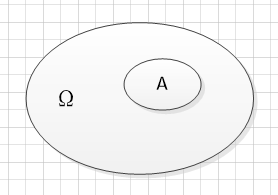
\includegraphics[scale=0.4]{geometry}
\end{frame}

\begin{frame}
\begin{example}
	(会面问题)甲、乙两人约定在6时到7时之间在某处会面,并约定先到者应等候另一个人一刻钟,过时即可离去。求两人能会面的概率。\\
	如图,以x,y表示甲乙两人,则两人能会面的充要条件是: $|x-y|\leq 15$\\
	$$P(A)=\frac{S_A}{S_\Omega}=\frac{60^2-45^2}{60^2}=\frac{7}{16}$$
	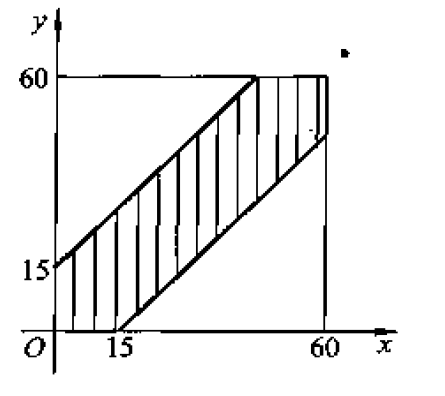
\includegraphics[scale=0.4]{geometry1}
\end{example}
\end{frame}

\section{条件概率}

\begin{frame}{概率的加法公式与条件概率}
如果有两个随机事件$A,B\in\mathcal{F}$,有如下加法公式:
\[P(A\cup B)=P(A)+P(B)-P(AB)\]
特备地,当$A,B$是补不相容的两个事件, 即$A\cap B=\emptyset$时, 有
\[P(A\cup B)=P(A)+P(B)\]

\begin{columns}
	\column{0.4\textwidth}%<1->
	\[P(A|B)=\frac{S_{AB}}{S_B}=\frac{S_{AB}/S_\omega}{S_B/S_\omega}=\frac{P(AB)}{P(B)} \]
	\column{0.4\textwidth}%<1->
	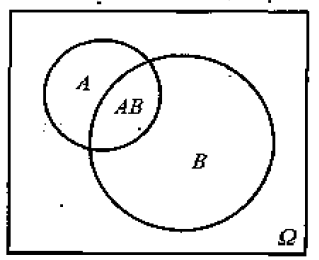
\includegraphics[scale=0.2]{P(AB)}
\end{columns}
\end{frame}

\begin{frame}{条件概率}
\begin{definition}
	若$\Omega,\mathcal{F},P$是一个概率空间,$B\in\mathcal{F}$, 且$P(B)>0$,则对任意的$A\in\mathcal{F}$,称
	$$P(A|B)=\frac{P(AB)}{P(B)}$$
	为在已知事件B发生的条件下,事件A发生的条件概率。
\end{definition}

\begin{columns}%0.6 0.4表示相对比例
	\column{0.4\textwidth}%<1->
\[P(A|B)=\frac{S_{AB}}{S_B}=\frac{S_{AB}/S_\omega}{S_B/S_\omega}=\frac{P(AB)}{P(B)} \]
	\column{0.4\textwidth}%<1->
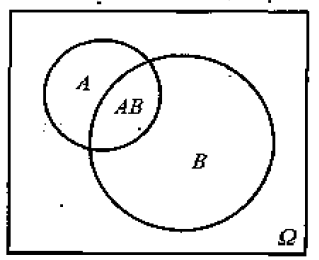
\includegraphics[scale=0.2]{P(AB)}
\end{columns}
\end{frame}

\begin{frame}{条件概率的性质及其推论}
\begin{block}{条件概率$P(\bullet|B)$的具备概率的三个基本性质}
	\begin{enumerate}
		\item 非负性: 对任意的$A\in F, P(A|B)\ge 0$;
		\item 规范性: $P(\Omega|B)=1$;
		\item 可列加性: 对任意的一列两两互不相容的事件$A_i(i=1,2,\dots)$, 有
		\[P\left[\bigcup\limits_{i=1}^{+\infty}(A_i|B)\right]=\sum\limits_{i=1}^{+\infty}P(A_i|B) \]
	\end{enumerate}
\end{block}
\begin{corollary}
概率的乘法公式:  $P(AB)=P(B)P(A|B)$
\end{corollary}

\begin{corollary}
	$P(A_1A_2\cdots A_n)=P(A_1)P(A_2|A_1)P(A_3|A_1A_2)\cdots P(A_n|A_1A_2\cdots A_{n-1})$
\end{corollary}
\end{frame}

\begin{frame}
\begin{example}
	一个家庭中有两个小孩,已知其中有一个是女孩,问这时另一个小孩也是女孩的概率有多大?\\
	$\Omega=$\{(男,男),(男,女),(女,男),(女,女)\}\\
	$A=$\{已知有一个是女孩\}=\{(男,女),(女,男),(女,女)\}\\
	$B=$\{另一个也是女孩\}=\{(女,女)\}\\
	于是所求概率为\\
	$P(B|A)=\frac{P(AB)}{P(A)}=\frac{1/4}{3/4}=\frac{1}{3}$
\end{example}
\end{frame}

\begin{frame}
差事件、条件事件或由差事件及条件事件复合而成的事件的概率均可化为$P(A),P(B),P(AB)$的形式。
例如
\[P(\overline{A\cup B})=1-P(A\overline{B})=1-[P(A)-P(AB)]=1-P(A)+P(AB) \]
\[P(A|\overline{B})=\frac{P(A)-P(AB)}{1-P(B)} \]
\begin{example}
	有外形相同的球分装在三个盒子,每盒10个。其中第一个盒子中7个球标有字母A,3个球标有字母B; 第二个盒子中有红球和白球各5个; 第三个盒子中则有红球8个,白球2个。试验按如下规则进行: 先在第一个盒子中任取一个球,若取得标有字母A的球,则在第二个盒子中任取一个球; 若第一次取得标有字母B的球,则在第三个盒子中任取一个球。如果第二次取出的是红球,则称试验成功。求试验成功的概率。
\end{example}
\end{frame}

\begin{frame}
\begin{solution}
	令$A=$\{从第一个盒子取得标有字母A的球\},$B=$\{从第一个盒子取得标有字母B的球\},$R=$\{第二次取出的球是红球\},$W=$\{第二次取出的球是白球\}。\\
	则容易球得: $P(A)=\frac{7}{10}, P(B)=\frac{3}{10}, P(R|A)=\frac{1}{2},P(W|A)=\frac{1}{2},P(R|B)=\frac{4}{5},P(W|B)=\frac{1}{5}$\\
	于是,试验成功的概率为
	\begin{align*}
	P(R)=P(R\cap\Omega)&=P[R\cap(A\cup B)]\\
	&=P(RA\cup RB)=P(RA)+P(RB)\\
	&=P(R|A)\cdot P(A)+P(R|B)\cdot P(B)\\
	&=\frac{1}{2}\cdot\frac{7}{10}+\frac{4}{5}\cdot\frac{3}{10}=0.59
	\end{align*}
	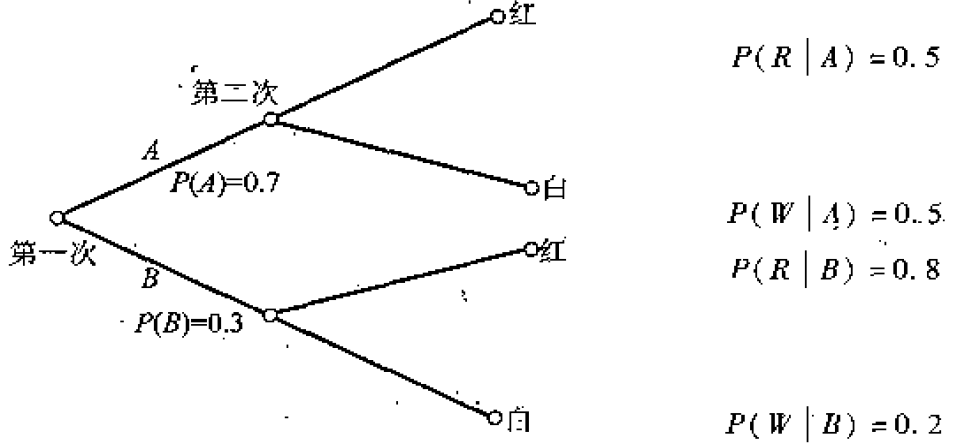
\includegraphics[scale=0.18]{tree}
\end{solution}
\end{frame}

\begin{frame}{概率树/全概率公式}
概率树思想:为了求解复杂事件的概率,往往可以先把它分解成两个(或若干个)互不相容的较简单的事件之并。求出这些较简单事件的概率,在利用加法公式即得所要求的复杂事件的概率。把这个方法一般化,便的到下述定理。
\begin{theorem}
	设$B_1,B_2,\cdots$是一列互不相容的事件,且有
	\[\bigcup_{i=1}^{+\infty}B_i=\Omega,P(B_i)>0 \]
	则对任一事件A,有
	\[P(A)=\sum_{i=1}^{+\infty}P(B_i)P(A|B_i) \]	
\end{theorem}
\end{frame}

\begin{frame}{概率树/全概率公式}
\begin{proof}
	\begin{align*}
	P(A)&=P(A\cap\Omega)=P[A\cap(\bigcup_{i=1}^{+\infty}B_i)]\\
	&=P[\bigcup_{i=1}^{+\infty}(AB_i)]=\sum_{i=1}^{+\infty}P(AB_i)\\
	&=\sum_{i=1}^{+\infty}P(B_i)P(A|B_i)
	\end{align*}
\end{proof}
\end{frame}

\begin{frame}
\begin{example}
	某工厂有4条流水线生产同一种产品, 该4条流水线的产品分别占总产量的15\%, 20\%, 30\%, 35\%, 又这4条流水线的不合格品率依次为0.05, 0.04, 0.03及0.02. 现从出厂产品中任取一件, 问(1) 恰好抽到不合格品的概率为多少? (2) 第4条流水线应承担的责任?
\end{example}
\end{frame}

\begin{frame}[shrink]
解: (1) 令
\begin{align*}
A&=\{\text{任取一件,恰好抽到不合格品} \}\\
B&=\{\text{任取一件,恰好抽到第$i$条流水线的产品}, (i=1,2,3,4) \}
\end{align*}
于是由全概率公式可得
\begin{align*}
P(A)&=\sum\limits_{i=1}^4P(B_i)P(A|B_i)=0.15\times 0.05+0.20\times 0.04+0.30\times 0.03+0.35\times 0.02\\
&=0.0315=3.15\%
\end{align*}
实际上,$P(A|B_i)$可以从过去生产的产品中统计出来,称为先验概率。\\
(2) 从概率论的角度考虑可以按$P(B_i|A)$的大小来追究第$i$条$i=1,2,3,4$流水线的责任。\\
$P(AB_4)=P(B_4)P(A|B_4)=0.35\times 0.02=0.007$\\
由条件概率的定义知
\begin{align*}
P(B_4|A)=\frac{P(AB_4)}{P(A)}=\frac{P(B_4)P(A|B_4)}{\sum\limits_{i=1}^4P(B_i)P(A|B_i)}=\frac{0.007}{0.0315}\approx=0.222
\end{align*}
\end{frame}

\begin{frame}{贝叶斯(Bayes)公式}
\begin{theorem}
	若$B_1, B_2, \dots$为一系列互不相容的事件, 且
	\[\bigcup\limits_{i=1}^{+\infty}B_i=\Omega \]
	\[P(B_i)>0, i=1,2,\dots \]
	则对任一事件A, 有
	\[P(B_i|A)=\frac{P(B_i)P(A|B_i)}{P(A)}=\frac{P(B_i)P(A|B_i)}{\sum\limits_{j=1}^{+\infty}P(B_j)P(A|B_j)}, \quad i=1,2,\dots \]
\end{theorem}
$P(B_i)$是试验以前就已经知道的概率---\textbf{先验(先于试验)概率}。\\
条件概率$P(B_i|A)$反映了试验以后,对A发生的``来源''的各种可能性的大小---\textbf{后验概率}。
\end{frame}

\begin{frame}{相互独立事件}
条件概率: $P(B|A)=\frac{P(AB)}{P(A)}$\\
一般的概率乘法公式: $P(AB)=P(A)P(B|A)$\\
如果``事件B发生与否不受事件A的影响'': $P(B)=P(B|A)$\\
乘法公式变为: $P(AB)=P(A)P(B)$
\begin{definition}
对任意的两个事件A,B,若
\[P(AB)=P(A)P(B)\]
成立,则称事件A,B是相互独立的,简称为独立的。	
\end{definition}
\begin{block}{依这个定义,不难验证:}
	若A与B相互独立,则$\{\emptyset,A,\overline{A},\Omega\}$中的任意一个与$\{\emptyset,B,\overline{B},\Omega\}$中的任意一个仍相互独立。
\end{block}
\end{frame}

\begin{frame}[shrink]
		分别掷两枚均匀的硬币,令
		\begin{align*}
		A=\{\text{硬币甲出现正面} \}\quad	B=\{\text{硬币乙出现正面} \}
		\end{align*}
		验证事件$A,B$是相互独立的。
 \begin{proof}
			$$\text{样本空间}=\{\text{(正,正),(正,反),(反,正),(反,反)}\} $$
			共还有4个基本事件,它们是等可能的,各有概率为1/4,而\\
			\begin{align*}
			A&=\{\text{(正,正),(正, 反)}\} \\
			B&=\{\text{(正,正),(反, 正)}\} \\
			AB&=\{\text{正,正}\}
			\end{align*}
			由此知 \[P(A)=P(B)=\frac{1}{2}\]
			这时有 \[P(AB)=\frac{1}{4}=P(A)P(B)\]
			成立,所以A, B事件是相互独立的。
 \end{proof}
\end{frame}

\begin{frame}{伯努利(Bernoulli)概型}
如果试验E只有两个可能的结果: $A$及$\overline{A}$, 并且$P(A)=p,P(\overline{A})=1-p=q$其中$0<p<1$, 把E独立地重复$n$次的试验就构成了一个试验,这个试验称作\textbf{$n$重伯努利(Bernoulli)试验}, 简称\text{伯努利(Bernoulli)试验}或\textbf{伯努利(Bernoulli)概型},并记作$B^n$.\\
例如, ``一次抛掷n枚相同硬币''的试验就可以看作是一个n重伯努利试验。
一个伯努利试验的结果记作:
$$\omega=(\omega_1,\omega_2,\dots,\omega_n)$$
其中的$\omega_i(1\le i\le n)$或者为$A$或者为$\overline{A}$,因而这样的$\omega$共有$2^n$个。他们的全体就是这个伯努利试验的样本空间$\omega$。
\begin{align*}
B_k &=\{ \text{$n$重伯努利试验中事件A出现$k$次} \}\\
P(B_k)&=C_n^kp^kq^{n-k},0\le k\le n
\end{align*}
\end{frame}

\section{随机变量}

\begin{frame}
\begin{definition}
	设$(\Omega,\mathcal{F},P)$是一概率空间,$x(\xi)|\xi\in\Omega$是定义在$\Omega$上的单值实函数,如果对任一实数$x$, 集合$\{x(\xi)\le x\}\in\mathcal{F}$, 则称$x(\xi)$为$(\Omega,\mathcal{F},P)$上的一个\textbf{随机变量}。
	
	随机变量$x(\xi)$的定义域为样本空间$\Omega$,它的值域是实数R。所有随机变量$x(\xi)$实际上是一个映射,这个映射为每个来自概率空间的结果(样本点)$\xi$赋予一个实数$x$。这种映射必须满足条件:
	\begin{itemize}
		\item[(1)] 对任一$x$,集合$\{x(\xi)\le x\}$是这个概率空间中的一个事件,并有确定的概率$P\{x(\xi)\le x\}$;
		\item[(2)] $P\{x(\xi)=\infty \}=0$, $P\{x(\xi)=-\infty \}=0$
	\end{itemize}
	\begin{block}{Notes}
		随机变量$x(\xi)$就是试验结果(即样本点)和实数之间的一一对应关系。虽然在试验之前不能肯定随机变量$x(\xi)$会取哪一个数值,但是对于任一实数$a$, 我们可以研究$\{x(\xi)=a \}$发生的概率, 也就是$x(\xi)$取值的统计规律。
	\end{block}
\end{definition}
\end{frame}

\begin{frame}
关于随机变量(及向量)的研究,是概率论的中心内容.这是因为,对于一个随机试验,我们所关心的往往是与所研究的特定问题有关的某个或某些量,而这些量就是随机变量.

也可以说:\textbf{随机事件}是从静态的观点来研究随机现象,而\textbf{随机变量}则是一种动态的观点,一如数学分析中的常量与变量的区分那样.变量概念是高等数学有别于初等数学的基础概念。同样,概率论能从计算一些孤立事件的概念发展为一个更高的理论体系,其基础概念是随机变量。
\end{frame}

\begin{frame}
\begin{example}
	抛硬币试验中,H表示正面,T表示反面,样本空间$\Omega=\{H,T\}$,H与T不是数量,不便于计算及理论的研究,因而引入以下变量$\xi$,
	$$x=x(\xi)=
	\begin{cases}
	0, &\xi=T\\
	1, &\xi=H
	\end{cases}
	$$
\end{example}  
\end{frame}

\begin{frame}
\begin{definition}[随机变量]
设随机试验E的样本空间是$\Omega=\{\xi\}$, 若对于每一个$\xi\in\Omega$,有一个实数$x(\xi)$与之对应,即$x(\xi)$是定义在$\Omega$上的单值函数,称为随机变量。
\end{definition}
\begin{figure}[htbp]
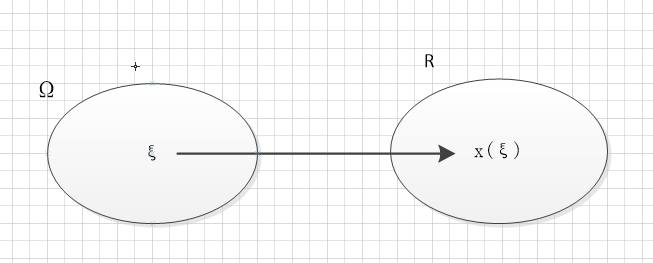
\includegraphics[scale=0.3]{xi_map}
\end{figure}
\begin{itemize}
\item 可用随机变量$x(\xi)$描述事件。\\
例掷一颗骰子(色子),设出现的点数记为随机事件A,表示``掷出的点数大于3''的事件A,可表示为``$x(\xi)>3$''。反过来,A的一个变化范围表示一个随机事件:``$2<x(\xi)<5$''表示事件``掷出的点数大于2且小于5''。
\item 随机变量随着试验的结果而取不同的值,在试验之前不能确切知道它取什么值,但是随机变量的取值有一定的统计规律性---概率分布。
\end{itemize}
\end{frame}

\begin{frame}{离散型随机变量}
\begin{definition}[离散型随机变量]
	定义在样本空间$\Omega$上,取值于实数域$\mathbb{R}$,且只取有限个或可列个值的变量$x=x(\xi)$, 称作是\textbf{一维(实值)离散型随机变量}。\\
\end{definition}
\begin{block}{``可列个''值}
	所谓``可列个''值,是指这个变量所取的值可依某种次序一一列举,排成一列。例如自然数全体就是可列的。
\end{block}
\end{frame}

\begin{frame}
\begin{example}
	设$\Omega=$\{某公司2018年对某险种售出的保单\}, 对$\xi\in\Omega$, 令
	\[x(\xi)=\xi\text{在一年中的索赔次数}\]
	则$x(\xi)$是$\Omega$上的一个一维离散型随机变量, $x(\xi)$的可能取值范围为$\{0,1,2,\dots\}$。 在试验(即签定某一份保单)之前,并不能断定$x$会取哪一个值,但是我们可以知道$(x=0),(x=1),\dots$这些事件发生的概率(也就是在总体中所占的比例)$P[x(\xi)]$。\\
	离散型随机变量$x(\xi)$的可能取值为$a_i(i=1,2,\dots)$, 相应的取值$a_i$的概率$P(x(\xi)=a_i)=p_i$,写成如下表格形式, 制表称为随机变量$x(\xi)$的\textbf{分布列},也称为\textbf{分布列},简称\textbf{分布}。\\
	\centering
	\begin{tabular}{|c|c|c|c|}
		\hline 
		$x(\xi)$ & $a_1$ & $a_2$ & $\cdots$\\ 
		\hline 
		$P[x(\xi)]$ & $P[x(\xi)=a_1]$ & $P[x(\xi)=a_2]$ & $\cdots$\\ 
		\hline 
	\end{tabular} 
\end{example}
\end{frame}

\begin{frame}
\begin{example}
	在$n=5$的伯努利试验中,设事件A在一次试验中出现的概率为$p$,即$P(A)=p,P(\overline{A}=q=1-p)$, 令
	\[x(\xi)=\text{5次试验中事件A出现的次数}\]
	则
	\[P[x(\xi)=k]=C_5^kp^kq^{5-k} \]
	\centering
		\begin{tabular}{|c|c|c|c|c|c|c|}
		\hline 
		$x(\xi)$ & 0 & 1 & 2 & 3 & 4 & 5\\ 
		\hline 
		$P[x(\xi)]$ & $q^5$ & $5pq^4$ & $10p^2q^3$ & $10p^3q^2$ & $5p^4q$ & $p^5$\\	\hline 
	\end{tabular} 	
\end{example}
\end{frame}


\begin{frame}{离散型随机变量$\xi$的分布列的性质}
\begin{block}{离散型随机变量$\xi$的分布列}
	\begin{tabular}{|c|c|c|c|}
		\hline 
		$\xi$ & 0 & 1 & $\cdots$\\ 
		\hline 
		$P(\xi)$ & $p_1$ & $p_2$ & $\cdots$\\ 
		\hline 
	\end{tabular} 
\end{block}

由概率的性质可知,任一离散型随机变量的分布$\{p_i\}$都有下述两个性质:
\begin{enumerate}
	\item $p_i\ge 0,i=1,2,...$
	\item $\sum\limits_{i=1}^{+\infty}{p_i}=1$.
\end{enumerate}
反过来,任意一个具有以上两个性质的数列$\{p_i\}$,都有资格作为某一个随机变量的分布列。
\end{frame}

\begin{frame}
分布列不仅明确地给出了$(\xi=a_i)$的概率,而且对于任意一个的实数a,b,事件$(a\le\xi\le b)$发生的概率均可由分布列算出,因为
\[(a\le\xi\le b)=\bigcup_{a\le\xi\le b}(\xi=a_i)\]
于是由概率的可列加性有
\[P(a\le\xi\le b)=\sum_{i\in I_{a,b}}P(\xi=a_i)=\sum_{i\in I_{a,b}}p_i\]
其中$I_{a,b}=\{i:a\le a_i\le b\}$,即使对$\mathbb{R}$中更复杂可列的集合$B$,也有
\[P(\xi\in B)=\sum_{i\in I(B)}P(\xi=a_i)=\sum_{i\in I(B)}p_i\]
其中$I(B)=\{i:a_i\in B\}$\\
由知此可,$x(\xi)$取各种值的概率都可以由它的分布列通过计算而得到。
\begin{block}{}
	分布列全面地描述了离散型随机变量$x(\xi)$的统计规律。
\end{block}
\end{frame}

\section{几种重要的离散型随机变量的分布}

\begin{frame}
\begin{block}{二项分布}
	若试验E只有两种可能结果,一种是事件A出现,另一种是事件$\overline{A}$出现,$P(A)=p$, 称试验E为伯努利(Bernoulli)试验。现将试验E独立重复n次,若用$\xi$表示事件A出现的次数,在这n重伯努利试验中,事件A恰好出现k次的概率为
	\[P\{\xi=k\}=C_{n}^{k}p^{k}(1-p)^{n-k},\qquad k=0,1,2,\dots,n\]
\end{block}
\begin{definition}[二项分布]
	若$\xi$的概率分布是
	\[P\{\xi=k\}=C_{n}^{k}p^{k}(1-p)^{n-k},\qquad k=0,1,2,\dots,n\]
	则称$\xi$服从参数为n,p的二项分布,记作$\xi\sim B(n,p)$。
\end{definition}
\begin{block}{Notes}
	n次伯努利试验是相互独立的事件,就是试验的结果是相互独立的。
\end{block}
\end{frame}

\begin{frame}
一个伯努利试验的结果(样本点)为:
\[\xi=(\xi_1,\xi_2,\dots,\xi_n)\]
其中的$\xi_i(1\le i\le n)$或者是$A$或者是$\overline{A}$,因而这样的$\xi$共有$2^n$个,它们的全体就是这个伯努利试验的样本空间$\Omega$,对于$\xi=(\xi_1,\xi_2,\dots,\xi_n)\in\Omega$, 如果$\xi_i(1\le \xi\le n)$中有$k$个为$A$, 则必有$n-k$个为$\overline{A}$,于是由独立性即得
\[P(\xi)=p^k(1-p)^{n-k}\]
如果要求``$n$重伯努利试验中事件$A$出现$k$次''这一事件的概率,为此记
\[B_k=\{\text{$n$重伯努利试验中事件$A$出现$k$次}\}\]
由概率的有限可加性记得
\[P(B_k)=\sum_{\xi\in B_k}P(\xi)\]
对于$\xi\in B_k$,已知$P(\xi)=p^k(1-p)^{n-k}$, 而$B_k$中这样的$\xi$共有$C_{n}^{k}$个,所以
\[P(B_k)=C_n^k p^k(1-p)^{n-k},\qquad 0\le k\le n\]
\end{frame}

\begin{frame}
\begin{example}
   抛掷一枚硬币,出现正面的概率$p=\frac{1}{2}$,``抛掷n枚相同的硬币,恰好出现k个正面"这一事件的概率, 就是n重伯努利试验。\\
   \[P(\xi=k)=C_n^kp^k(1-p)^{n-k}=C_n^k(\frac{1}{2})^n\]
\end{example}
\begin{example}
一批产品的废品率为0.03,进行20次独立重复抽样,求出现废品的频率为0.1的概率。\\
令$\xi$表示在这20次独立重复抽样中出现的废品数,则$\xi\sim B(20,0.03)$。于是
\[P\{\frac{\xi}{20}=0.1\}=P\{\xi=2\}=C_{20}^{2}0.03^{2}(0.97)^{18}\approx 0.0988\]
\end{example}
\end{frame}

\begin{frame}
金工车间由10台同类型的机床,每台机床配备的电动机功率为10千瓦,已知每台机床工作时,平均每小时实际开动12分钟,且开动与否是相互独立的。现因当地电力供应紧张,供电部门只提供50千瓦的电力给这10台机床。问这10台机床能够正常工作的概率为多大?\\
解 50千瓦电力可同时供给5台机床工作(开动),因而10台机床中同时开动的台数不超过5台时都可以正常工作。每台机床正常工作的概率$p=\frac{12}{60}=\frac{1}{5}$。设10台机床中正常工作的机床台数为$\xi$,则
\[P(\xi=k)=C_n^kp^k(1-p)^{n-k}=C_{10}^k(\frac{1}{5})^k(\frac{4}{5})^{10-k},\quad 0\le k\le 10 \]
于是同时正常工作着的机床台数不超过5台的概率为
\begin{align*}
P(\xi\le 5) &= \sum_{k=0}^{5}P(\xi=k)\\
&=\sum_{k=0}^{5}C_{10}^k(\frac{1}{5})^k(\frac{4}{5})^{10-k}\approx 0.994
\end{align*}
\end{frame}

\begin{frame}
某大学的校乒乓球队与数学系乒乓球队举行对抗赛。校队的实力比系队强,当一个校队的运动员与一个系队的运动员比赛时,校队运动员获胜概率为0.6。 校、系双方对抗赛有以下三种方案:\\
(1) 双方各出3人,比三局; (2) 双方各出5人,比五局; (3) 双方各出7人,比七局。\\
三种方案中均以比赛中得胜人数多得一方为胜利。问: 对系队来说,哪一种方案有利?
\begin{block}{}
	设系队得胜人数为$\xi$, 则在上述三种方案中,系队胜利的概率为:
	\begin{align*}
	(1) P(\xi\ge 2) &=\sum_{k=2}^{3}C_3^k(0.4)^k(0.6)^{3-k}\approx 0.352\\
    (2) P(\xi\ge 3) &=\sum_{k=3}^{5}C_5^k(0.4)^k(0.6)^{5-k}\approx 0.317\\
    (3) P(\xi\ge 4) &=\sum_{k=4}^{7}C_7^k(0.4)^k(0.6)^{7-k}\approx 0.290\\
	\end{align*}
\end{block}
\end{frame}

\begin{frame}{随机变量的分布函数}
\begin{definition}
	设$\xi$是随机变量, 对$\forall x\in\mathbb{R}$, 称函数
	\[F(x)=P\{x(\xi)\le x\}\]
	为随机变量$x(\xi)$的(累积)分布函数[(cumulative) distribution function]。
\end{definition}
\begin{block}{分布函数性质}
\begin{enumerate}
	\item 单调不减性: 对$\forall x_1<x_2$, 恒有$F(x_1)\le F(x_2)$
	\item 规范性: $F(-\infty)=\lim\limits_{x\to -\infty}F(x)=0$, $F(+\infty)=\lim\limits_{x\to +\infty}F(x)=1$
	\item 右连续性: 对$\forall x_0$, 恒有$F(x_0+0)=\lim\limits_{x\to x_0^+}F(x)=F(x_0)$
\end{enumerate}
\end{block}
\end{frame}

\begin{frame}{随机变量的概率密度函数}
\begin{definition}
	设连续随机变量$x(\xi)$的一维累积分布函数为$F(x)$, 如果$F(x)$对$x$的一阶导数存在,则有
	\[p(x)\mathop{=}^{def}\frac{dF(x)}{dx}\]
	式中, $p(x)$称为随机变量$x(\xi)$的一维概率密度函数, 简称概率密度函数(probability density function,p.d.f)
\end{definition}
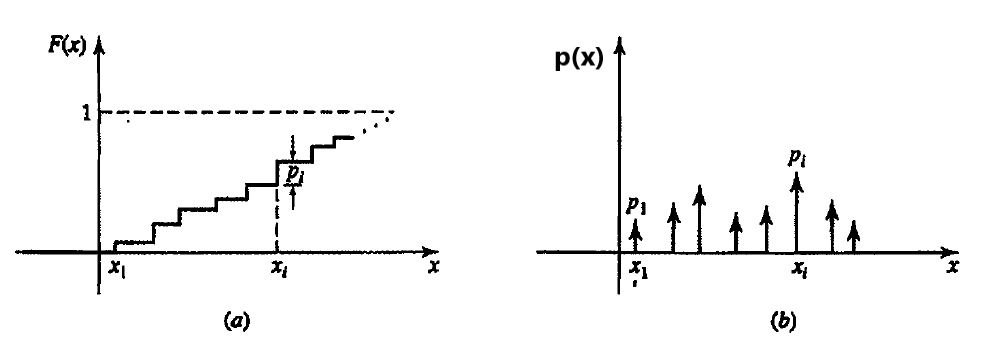
\includegraphics[scale=0.4]{pi}
\end{frame}

\begin{frame}[shrink]
\frametitle{随机变量概率密度函数性质}
\begin{enumerate}
	\item 根据随机变量$x(\xi)$的$p(x)$与$F(x)$的关系, 有
	\[F(x)=\int_{-\infty}^{x}p(u)du\]
	\item 对所有$x$, p(x)是非负函数,即
	\[p(x)\ge 0,\quad -\infty<x<+\infty \]
	\item $p(x)$对$x$的全域积分结果等于1, 一般表示为
	\[\int_{-\infty}^{\infty}p(x)dx=1\]
	\item 随机变量$x(\xi)$落在区间$[x_1,x_2]$内的概率为
	\[P\{x_1\le x(\xi)\le x_2\}=F(x_2)-F(x_1)=\int_{x_1}^{x_2}p(x)dx\]
\end{enumerate}
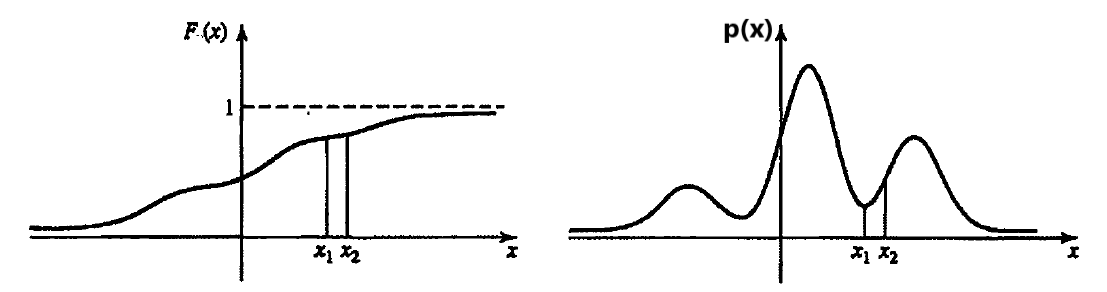
\includegraphics[scale=0.3]{Fx-px2}
\end{frame}

\begin{frame}[shrink]
抛掷一枚硬币: 样本空间: $\Omega=\{h,t\}$, $h$表示正面, $t$表示反面。正面的概率$p$, 反面的概率$q$. 定义随机变量$x(\xi),\xi\in \Omega$满足:
	\[x(\xi=h)=x(h)=1\qquad x(\xi=t)=x(t)=0,\]
	求$F(x)$,其中: $-\infty<x<\infty$.\\
	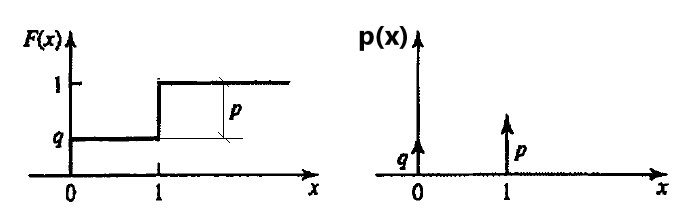
\includegraphics[scale=0.4]{coin-tossing}\\
	如果$x\ge 1$, 则$x(h)=1\le x$, 且$x(t)=0\le x$, 有
	\[F(x)=P\{x(\xi)\le x \}=P\{h,t\}=1\qquad x\ge 1 \] 
    如果$0\le x<1$, 则$x(h)=1> x$, 且$x(t)=0\le x$, 有
    \[F(x)=P\{x(\xi)\le x \}=P\{t\}=q \qquad 0\le x<1 \] 
    如果$x<0$, 则$x(h)=1> x$, 且$x(t)=0> x$, 有
    \[F(x)=P\{x(\xi)\le x \}=P\{\emptyset\}=0 \qquad x<0 \] 
\end{frame}

\begin{frame}[shrink]
事件A, 试验的样本空间: $\Omega=\{A,\overline{A},\emptyset \}$. 定义随机变量$x(\xi)$,
满足:
\begin{align*}
	x(\xi)=1, &\quad \xi\in A\\
	x(\xi)=0, &\quad \xi\in\overline{A}
\end{align*}
$P(A)=p,P(\overline{A})=q=1-p$
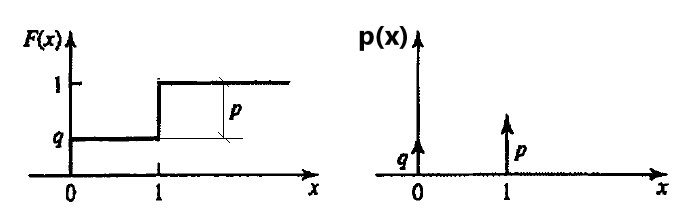
\includegraphics[scale=0.4]{coin-tossing}\\
如果$x\ge 1$, 则$\{x(\xi)\le x\}=\{\Omega \}$, 有
\[F(x)=P\{x(\xi)\le x \}=P\{\Omega \}=1\qquad x\ge 1 \] 
如果$0\le x<1$, 则$\{x(\xi)\le x\}=\{\overline{A}\}$, 有
\[F(x)=P\{x(\xi)\le x \}=P\{\overline{A}\}=q \qquad 0\le x<1 \] 
如果$x<0$, 则$\{x(\xi)\le x\}=\{\emptyset\}$, 有
\[F(x)=P\{x(\xi)\le x \}=P\{\emptyset\}=0 \qquad x<0 \] 
\end{frame}

\begin{frame}[shrink]
抛掷两枚硬币: 随机变量$x(\xi)$表示正面数目。求$F(x)$.\\
样本空间: $\Omega=\{HH,HT,TH,TT\}$, $H$表示正面, $T$表示反面。\\
随机变量$x(\xi)$: $x(HH)=2,\quad x(HT)=1, \quad x(TH)=1, \quad x(TT)=0$
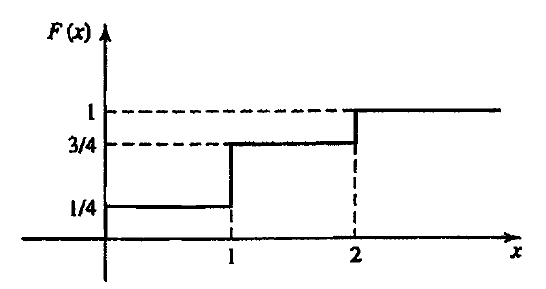
\includegraphics[scale=0.3]{coin-tossing2}\\
如果$x\ge 2$, $\{x(\xi)\le x\}=\Omega \Rightarrow F(x)=1$ \\
如果$1\le x<2$, $\{x(\xi)\le x\}=\{TT,HT,TH\} \Rightarrow F(x)=P\{TT\}+P\{HT\}+P\{TH\}=\frac{3}{4}$ \\
如果$0\le x<1$, $\{x(\xi)\le x\}=\{TT\} \Rightarrow F(x)=P\{TT\}=P(T)P(T)=\frac{3}{4}$ \\
如果$x<0$, $\{x(\xi)\le x \}=\emptyset \Rightarrow F(x)=0$ \\
当$x=1$, $P\{x(\xi)=1\}=F(1)-F(1^{-})=3/4-1/4=1/2$
\end{frame}

\begin{frame}[shrink]
掷一枚骰子: 样本空间: $\Omega=\{f_1,f_2,f_3,f_4,f_5,f_6\}$。定义随机变量$x(\xi),\xi\in \Omega$满足:$x(f_i)=10i$
求$F(x)$,其中: $-\infty<x<\infty$.\\
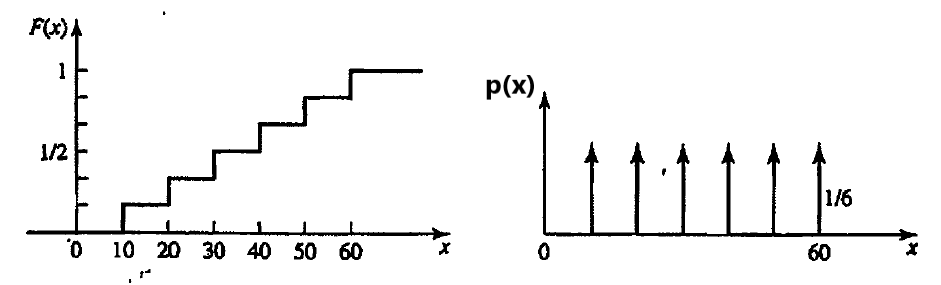
\includegraphics[scale=0.4]{die}
\begin{align*}
F(100)&=P\{x(\xi)\le 100 \}=P(\Omega)=1\\
F(35)&=P\{x(\xi)\le 35 \}=P\{f_1,f_2,f_3 \}=\frac{3}{6} \\
F(30.01)&=P\{x(\xi)\le 30.01 \}=P\{f_1,f_2,f_3 \}=\frac{3}{6} \\
F(30)&=P\{x(\xi)\le 30 \}=P\{f_1,f_2,f_3 \}=\frac{3}{6} \\
F(29.9)&=P\{x(\xi)\le 35 \}=P\{f_1,f_2 \}=\frac{2}{6} \\
\end{align*}
\end{frame}

\begin{frame}
\begin{columns}
	\column{0.5\textwidth}
	均匀分布随机变量$x(t)=t,0<t<T$\\
	$P\{t_1\le t\le t_2\}=\frac{t_2-t_1}{T},0<t_1<t_2<T$\\
	如果$x> T$, 有
	\[F(x)=P\{x(t)\le x \}=P\{0\le t\le T \}=P(\Omega)= 1\qquad x> 1 \] 
	如果$0\le x\le T$, 有
	\[F(x)=P\{x(t)\le x \}=P\{0\ge t\le x\}=\frac{x}{T} \qquad 0\le x\le 1 \] 
	如果$x<0$, 有
	\[F(x)=P\{x(t)\le x \}=P\{\emptyset\}=0 \qquad x<0 \] 
	\column{0.4\textwidth}
	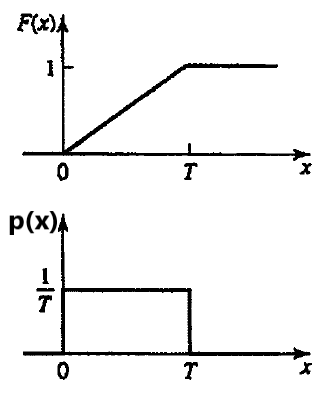
\includegraphics[scale=0.4]{xt}
\end{columns}
\end{frame}

\begin{frame}
\begin{columns}
	\column{0.5\textwidth}
	定义随机变量$x(\xi)$, 满足$\forall xi\in\Omega, x(\xi)=a$\\
	如果$x\ge a$, 则,$\forall \xi\in\Omega, x{\xi}=a\le x$,有
	\[F(x)=P\{x(\xi)\le x \}=P(\Omega)= 1\qquad x\ge a \] 
	如果$x<a$, 有
	\[F(x)=P\{x(t)\le x \}=P\{\emptyset\}=0 \qquad x<a \] 
	\column{0.4\textwidth}
	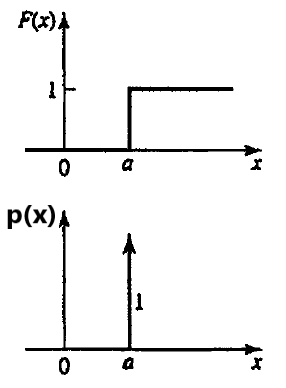
\includegraphics[scale=0.4]{a}
\end{columns}
\end{frame}

\begin{frame}[shrink]
非负实数集合$\{p_i\}$,$\forall i, i=1,2,\dots,\infty$满足, 
\begin{enumerate}
	\item $P\{x(\xi)=x_i\}=p_i$
	\item $\sum\limits_{i=1}^{\infty}p_i=1$
\end{enumerate}
求$F(x)$,其中: $-\infty<x<\infty$.\\
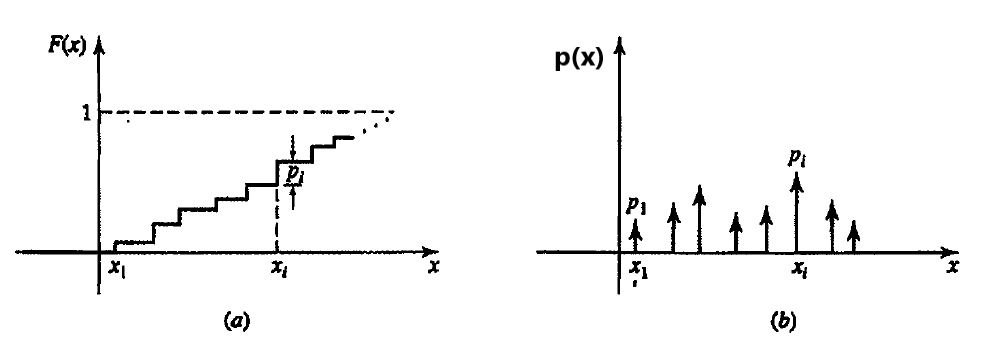
\includegraphics[scale=0.4]{pi}\\
对于$x_i\le x<x_{i+1}$, 我们有$\{x(\xi)\le x \}=\bigcup\limits_{x_k\le x}\{x(\xi)=x_k\}=\bigcup\limits_{k=1}^{i}\{x(\xi)=x_k\}$, 因此
\begin{align*}
F(x)=P\{x(\xi)\le x\}=\sum\limits_{k=1}^{i}p_k \qquad x_i\le x<x_{i+1}
\end{align*}
\end{frame}

\begin{frame}{离散型随机变量$x(\xi)$的$p(x)$}
\[P\{x(\xi)=x_i\}=F(x_j)-F(x_i^{-})=p_i\]
\[p(x)=\sum\limits_{i}p_i\delta(x-x_i) \]
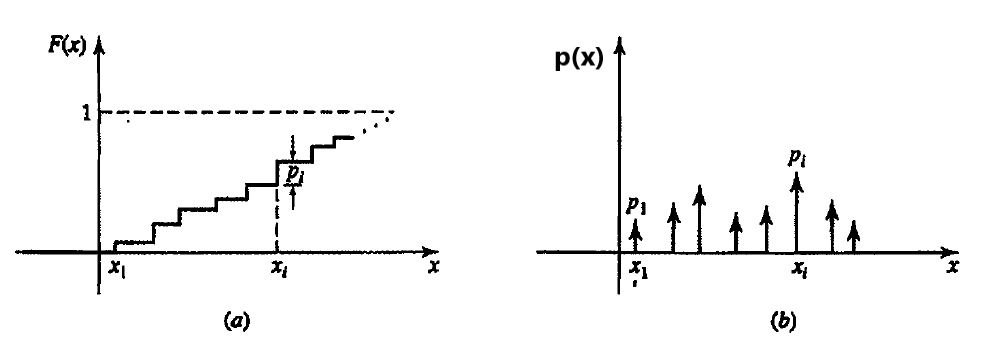
\includegraphics[scale=0.3]{pi}\\
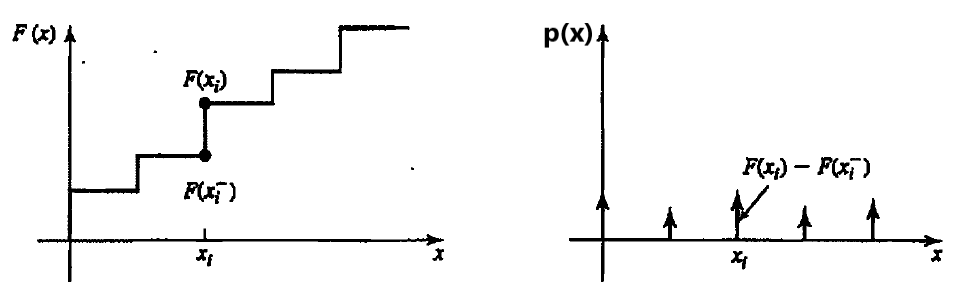
\includegraphics[scale=0.3]{Fx-px}
\end{frame}

\begin{frame}
\begin{example}
	某产品40件,其中次品3件,现从中任取3件。(1) 求取出的3件产品中所含次品数$\xi$的分布列; (2) 求取出的产品中至少有一件次品的概率; (3) 求$x(\xi)$的分布函数$F(x)$。
	\begin{block}{}
		(1) \begin{tabular}{ll}
			$P\{\xi=0\}=\frac{C_{37}^{3}}{C_{40}^{3}}=0.7865$ & $P\{\xi=1\}=\frac{C_{3}^{1}C_{37}^{2}}{C_{40}^{3}}=0.2022$ \\ 
			$P\{\xi=2\}=\frac{C_{3}^{2}C_{37}^{1}}{C_{40}^{3}}=0.0112$ & $P\{\xi=3\}=\frac{C_{3}^{3}}{C_{40}^{3}}=0.0001$ \\ 
		\end{tabular}\\ 
	   (2) $P\{\xi\ge 1\}=1-P\{\xi=0\}=1-0.7865=0.2135$\\
	   (3) 由分布函数定义得:
	   $F(x)=P\{x(\xi)\le x\} =
	   \begin{cases}
	   	0,      & x<0 \\
	   	0.7865, & 0\le x<1 \\
	   	0.9887, & 1\le x<2 \\
	   	0.9999, & 2\le x<3 \\
	   	1,      & x\ge 3
	   \end{cases} $
	\end{block}
\end{example}
\end{frame}

\begin{frame}
\begin{block}{解:}
		(1) \begin{tabular}{ll}
			$P\{\xi=0\}=\frac{C_{37}^{3}}{C_{40}^{3}}=0.7865$ & $P\{\xi=1\}=\frac{C_{3}^{1}C_{37}^{2}}{C_{40}^{3}}=0.2022$ \\ 
			$P\{\xi=2\}=\frac{C_{3}^{2}C_{37}^{1}}{C_{40}^{3}}=0.0112$ & $P\{\xi=3\}=\frac{C_{3}^{3}}{C_{40}^{3}}=0.0001$ \\ 
		\end{tabular}\\ 
		(2) $P\{\xi\ge 1\}=1-P\{\xi=0\}=1-0.7865=0.2135$\\
		(3) 由分布函数定义得:
		$F(x)=P\{x(\xi)\le x\} =
		\begin{cases}
		0,      & x<0 \\
		0.7865, & 0\le x<1 \\
		0.9887, & 1\le x<2 \\
		0.9999, & 2\le x<3 \\
		1,      & x\ge 3
		\end{cases} $
		\begin{columns}%0.6 0.4表示相对比例
			\column{0.4\textwidth}%<1->
			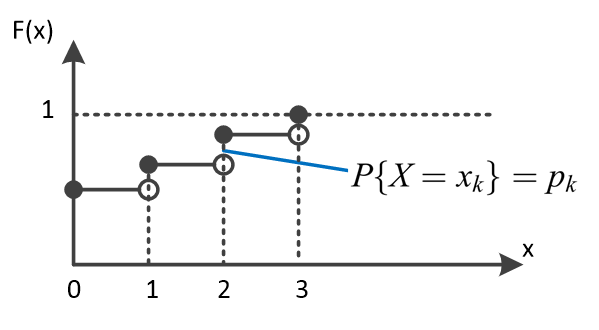
\includegraphics[scale=0.5]{fx}
			\column{0.6\textwidth}%<1->
			由$F(x)$的图示看到, $F(X)$是一个阶梯状的右连续函数($F(x+0)=F(x)$),在$x=k$处有跳跃,跃度为$\xi$在$x=k$处的概率。\\
            $F(k)-F(k-0)=P(\xi=k), k=0,1,2,3,\dots$			
	    \end{columns}
\end{block}
\end{frame}

\begin{frame}
\begin{columns}
	\column{0.4\textwidth}
	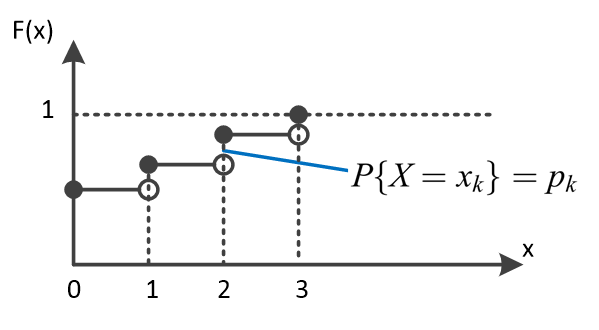
\includegraphics[scale=0.5]{fx}
	\column{0.6\textwidth}
	由随机变量$x(\xi)$的分布函数$F(x)$, 可以计算
	\begin{block}{}
		\begin{align*}
		P(x(\xi)\le x) &= F(x)\\
		P(x(\xi) = x) &= F(x)-F(x-0) \\
		P(x(\xi) < x) &= F(x-0) \\
		P(x(\xi) > x) &= 1- F(x) \\
		P(x(\xi) \ge x) &= 1-F(x-0)
		\end{align*}
		进一步,形如$\{x_1\le x(\xi)\le x_2\},\{x_1< x(\xi)< x_2\},\{x_1< x(\xi)\le x_2\}, \{x_1\le x(\xi)< x_2\}$等一些事件及它们经过有限次或可列次并、交、差运算以后的概率,都可以由$F(x)$算出来。
	\end{block}
 \end{columns}
\begin{block}{}
	$F(x)$全面地描述了随机变量$x(\xi)$地统计规律。既然分布函数能够描述一般的随机变量的统计规律,因而分布函数这个概念比分布列更重要。只不过对离散型随机变量来说,分布列比较方便。
\end{block}
\end{frame}

\begin{frame}{离散性随机变量的分布函数与分布列之间的关系}
\[F(x)=P(x(\xi)\le x)= \sum_{a_i\le x}P(x(\xi)=a_i)\]
\begin{columns}
	\column{0.4\textwidth}
	\begin{block}{离散型随机变量$\xi$的分布列}
		\begin{tabular}{|c|c|c|c|}
			\hline 
			$x(\xi)$    & $a_1$ & $a_2$ & $\cdots$\\ 
			\hline 
			$P(x(\xi))$ & $p_1$ & $p_2$ & $\cdots$\\ 
			\hline 
		\end{tabular} 
	\end{block}
	\column{0.4\textwidth}
	\begin{block}{离散型随机变量$\xi$的分布函数}
		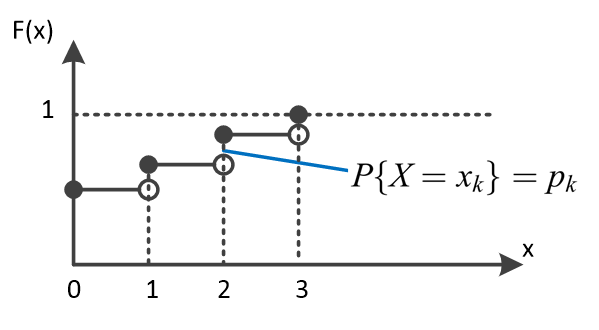
\includegraphics[scale=0.5]{fx}
	\end{block}
\end{columns}
\end{frame}

\begin{frame}
\begin{example}
	若$\xi$只取一个值$a$, 即有$P(\xi=a)=1$, 求$\xi$的分布函数$F(x)$.
\end{example}
\begin{block}{解}
	\[
	 F(x)=P(\xi\le x)= 
	 \begin{cases}
	 1, &x\ge a\\
	 0, &x<a
	 \end{cases}
	\]
	\begin{columns}
		\column{0.4\textwidth}	
		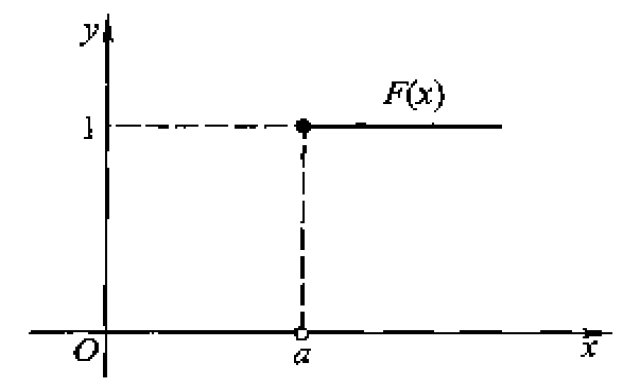
\includegraphics[scale=0.3]{fx1}
		\column{0.4\textwidth}
		如图所示,$F(x)$是一个右连续的、阶梯状的函数,在$x=a$处有一个跳跃,其跃度为
		\[1=P(\xi=a)\]
	\end{columns}
\end{block}
\end{frame}

\begin{frame}
\begin{example}
	等可能地在$[a,b]$上投点,所投的点落在$[a,b]$中的任一子区间$B=[c,d]$中的概率与$B$的长度$l_B$成正比,而与$B$在$[a,b]$中的位置无关。如果记``点落入$B$中"这一事件为$B$,则上述等可能性意味着
	\[P(B)=\frac{l_B}{b-a}=\frac{d-c}{b-a}\]
	如果投在$[a,b]$中的点的坐标为$\xi(a\le\xi\b)$令
	\[x(\xi)=\xi\qquad (a\le\xi\b)\]
	这样就得到一个随机变量$x(\xi)$,它的取值充满了整个区间$[a,b]$.
	对于任意一点$\xi_0$的概率为: 
	\[P(x(\xi)=\xi_0)=P(\xi=\xi_0)=\frac{l_{\xi_0}}{b-a}=0\]
	由于单点集的长度为零。
	因此用``分布列"研究随机变量$x(\xi)$的统计规律是行不通的。引入分布函数的概念。
\end{example}
\end{frame}

\begin{frame}
点落落入$B=[c,d]$区间的概率与$B$的长度$l_B$成正比,设$B=[c,d]\subset [a,b]$,就有
	\[P(c\le d)=P(\text{点落入$B$中})=P(B)=\frac{d-c}{b-a} \]
	因为$P(\xi =c)=0$,所以
	\[a\]
\end{frame}

%%%%%%%%%%%%%%%%%%%%%%%%%%%%%%%%%%%%%%%%%%%%%%%%%%%%%

注释的内容
\iffalse  %注释开始

\begin{frame}
n重伯努利试验k次成功的概率(二项分布):
\[P\{\xi=k\}=C_{n}^{k}p^{k}(1-p)^{n-k},\qquad k=0,1,2,\dots,n\]
特例:令二项分布的$n=1$, $k$只能取0或1,描述事件A发生的概率。

\begin{definition}[0--1分布]
	若$x(\xi)$的概率分布是\\
	\begin{center}
	\begin{tabular}{|c|c|c|}
		\hline 
		$\xi$ & 0 & 1\\ 
		\hline 
		$P(\xi)$ & $1-p$ & $p$\\ 
		\hline 
	\end{tabular} \\
	\end{center}
	则称$x(\xi)$服从参数$p$的0--1分布。
\end{definition}

\end{frame}

\begin{frame}
\begin{example}
	抛掷一枚硬币, $p=1-p=\frac{1}{2}$。\\
	\begin{tabular}{|c|c|c|}
		\hline 
		$\xi$ & 0(正面朝上) & 1(正面朝下)\\ 
		\hline 
		$P(\xi)$ & $0.5$ & $0.5$\\ 
		\hline 
	\end{tabular} 
\end{example}

\begin{example}
	一批产品的废品率为5\%, 从中任取一个进行检查, 若令$\xi$表示取得废品的数量,写出$\xi$的概率分布。\\
	\begin{tabular}{|c|c|c|}
		\hline 
		$\xi$ & 0 & 1\\ 
		\hline 
		$P(\xi)$ & $0.95$ & $0.05$\\ 
		\hline 
	\end{tabular} 
\end{example}
\end{frame}

\begin{frame}
在一个努利试验中,每次试验成功的概率为$p$,失败的概率为$1-p$,设试验进行到第k次才成功,试验结束。
第k次才成功,表明k-1次是的失败的,概率为$(1-p)^{k-1}$, 有独立性即得总的概率为$(1-p)^{k-1}p$。

\begin{definition}[几何分布]
	若$x(\xi)$的概率分布是
	\[P(\xi=k)=(1-p)^{k-1}p,\qquad (0<p<1,k=1,2,\dots)\]
	则称$x(\xi)$服从参数为$p$的几何分布,记作$\xi\sim G(p)$
\end{definition}
\end{frame}

\begin{frame}
\begin{example}
	社会上定期发行某种奖券,每券一元,中奖率为$p$,某人每次购买1张奖券, 如果没有中奖,下次继续购买一张,直到中奖为止。求该人购买奖券次数$\xi$的概率分布。\\
	令$A_k=$\{第$k$次购买的奖券中奖\}, $k=1,2,3,...$, \\
	则$P(A_k)=p,\quad P(\overline{A_k})=1-p$, \\
	由于$A_1,A_2,A_3,\dots$相互独立,于是:
	\begin{align*}
	P(\xi=1)&=P(A_1)=p\\
	P(\xi=2)&=P(\overline{A_1}A_1)=P(\overline{A_1})P(A_2)=(1-p)p\\
	P(\xi=3)&=P(\overline{A_1}\overline{A_2}A_3)=P(\overline{A_1})P(\overline{A_2})P(A_3)=(1-p)^{2}p\\
	\cdots\\
	P(\xi=k)&=P(\overline{A_1}\overline{A_2}\cdots\overline{A_{k-1}}A_k)=P(\overline{A_1})P(\overline{A_2})\cdots P(\overline{A_{k-1}})P(A_k)=(1-p)^{k-1}p
	\end{align*}
	$\implies \xi\sim G(p)$
\end{example}
\end{frame}

\begin{frame}
\begin{example}
	某射手命中率为$p,(0<p<1)$,现有五发子弹。射击一发,如果命中,即停止射击,否则再射击一次,依次类推,如用$\eta$表示他射击所用去的子弹数,求$\eta$的分布。\\
	当$(\eta=k),1\le k\le 4$时表示前$(k-1)$次射击均未命中。第$k$次才首次命中,依题意,每次射击是相互独立的。故$P(\eta=k| 1\le k\le 4)=(1-p)^{k-1}p$。而$(\eta=5)$时表示前4次射击均未命中,第5次射击后不管是否命中均要停止。故$P(\eta=k|k=5)=(1-p)^{k-1}p$。\\
	\begin{tabular}{|c|c|c|c|c|c|}
		\hline 
		$\eta$ & 1 & 2 & 3 & 4 & 5\\ 
		\hline 
		$P(\eta)$ & $p$ & $p(1-p)$ & $p(1-p)^2$ & $p(1-p)^3$  & $(1-p)^4$ \\ 
		\hline 
	\end{tabular} 
\end{example}
\end{frame}

\fi   %注释结束
 %概率论回顾全集备份
%%%%%%%%%%%%%%%%%%%%%%%%%%% ch2-StochasticProcess
\begin{frame}[shrink]
\frametitle{ch2.信号检测与估计理论的基础知识}
\framesubtitle{随机过程}
\tableofcontents[hideallsubsections]
\end{frame}

\section{随机过程的定义}

\begin{frame}{随机过程引例(1)}
\begin{example}
	考察$[0,t_0]$时间内某网站收到的访问次数$X(t_0)$, $X(t_0)$则是一个随机变量。
	\begin{itemize}
		\item 如果要长时间内该网站的访问次数,则需要让$t$变化起来,即$t$趋于无穷大,则$X(t)$是一簇随机变量.
		\item 此时$X(t)$是与时间有关系的随机变量, 称$\{X(t),t\in[0,\infty]\}$是随机过程。
	\end{itemize}	
\end{example}
\end{frame}

\begin{frame}{随机过程引例(2)}
\begin{example}
	具有随机初位相的简谐波
	\[X(t)=A\cos(\omega t+\Phi)\]
	其中$A,\omega$为常数,$\Phi$服从$[0,2\pi]$上的均匀分布。
	\begin{itemize}
		\item 由于初位相的随机性,在某时刻$t=t_0,X(t)$是一个随机变量.
		\item 若要观察任一时刻$t$的波形,则需要用一簇随机变量$X(t)$描述. 
		\item 称$\{X(t),t\in[0,\infty]\}$是随机过程。
	\end{itemize}	
\end{example}
\end{frame}

\begin{frame}{随机过程引例(3)}
\begin{columns}
	\column{0.6\textwidth}
	\begin{example}
		三次热噪声电压测量结果:固定$t$时刻电压,对应一个随机变量$v(t)$; 无限个$t$,则无限个电压---时间的函数族构成一随机过程。
	\end{example}
	\column{0.4\textwidth}
	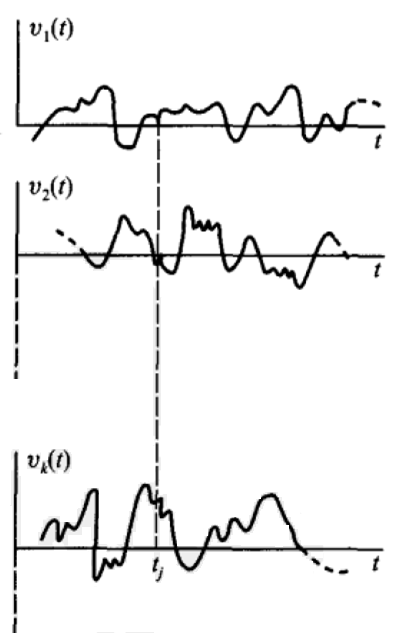
\includegraphics[scale=0.3]{vt}
\end{columns}
\end{frame}

\begin{frame}{随机过程引例(4)}
\begin{example}
	生物群体的增长问题.以$X_t$表示在时刻$t$某种生物群体的个数,则对每一个固定的$t,X_t$是一个随机变量。 
	\begin{itemize}
		\item 如果从$t=0$开始,每隔24小时对群体的个数观察一次,则对每一个$t$,$X_t$是一簇随机变量。记为$X_n,n=0,1,\dots$
		\item 若要观察任一时刻$t$的波形,则需要用一族随机变量$X(t)$描述. 
		\item 称$\{X_t,t=0,1,2,\dots\}$是随机过程。
	\end{itemize}	
\end{example}
\end{frame}

\begin{frame}{随机过程引例特点}
\begin{block}{以上例子的共同特点---随机现象在时间上的延展$\implies$\textbf{随机过程}}
	\begin{itemize}
		\item 给定一个$t$,就有一个随机变量$X(t)$与之对应。
		\item 概率论主要是以\textbf{一个或有限个随机变量}为研究对象的.
		\item 随机过程是概率论的``动力学''部分,研究对象为随时间演变的随机现象,通常会有\textbf{无穷多个随机变量}。
	\end{itemize}	
\end{block}
\end{frame}

\begin{frame}%{随机过程的定义}
\begin{definition}[随机过程]
	设$(\Omega,\mathcal{F},P)$是一概率空间, $T$是一实参数集,定义在$\Omega$和$T$上的二元函数$X(t,\xi)$
	\begin{enumerate}
		\item 固定$t_k\in T,X(t_k,\xi)$是概率空间上的\textbf{随机变量};
		\item 固定$\xi_i\in\Omega,X(t,\xi_i)$是概率空间上的\textbf{随机函数}(或称$X(t,\xi_i)$是对应于$\xi_i$的\textbf{样本函数})
	\end{enumerate}
    则称$\{X(t,\xi),t\in T,\xi\in \Omega \}$为一\textbf{随机过程},简记为$X(t)$,其中$t$和$\xi$均是变量。\\
	随机过程的定义域是实参数集$T$和样本空间$\Omega$。值域是实数集$\mathbb{R}$.
	\begin{itemize}
		\item 样本空间$\Omega$:一个随机试验所有可能出现的结果的全体,称为随机事件的样本空间。\\
		\item 事件域$\mathcal{F}$: 样本空间中的某些子集。
		\item
		参数集$T$表示时间或空间,通常的形式: $T=\{0,1,2,\dots \}$或$T=[a,b],T=[-\infty,\infty]$
	\end{itemize}
	\end{definition}
\end{frame}

\begin{frame}{用映射表示随机过程} 
\[X(t,\xi): T\times\Omega\to\mathbb{R} \]
\begin{enumerate}
	\item $X(\bullet,\bullet)$实质是定义在$T\times\Omega$上的二元单值函数;
	\item 固定$t\in T,X(t,\bullet)$是样本空间$\Omega$上的函数,即$X(t,\bullet)$为一\textbf{随机变量};
	\item 固定$\xi\in\Omega,X(\bullet,\xi)$是一个关于$t\in T$的函数,通常称为\textbf{样本函数},或称随机过程的\textbf{一次实现},所有样本函数的集合确定一随机过程。
	\item 随机过程$\{X(t,\xi)\}$可能取值的全体所构成的集合称为此随机过程的\textbf{状态空间},记作$S$。$S$中的元素称为\textbf{状态}。状态空间可以由复数、实数或更一般的抽象空间构成。
\end{enumerate}

记号$X(t,\xi)$有时记为$X_t(\xi)$或简记为$X(t)$。
\end{frame}

\begin{frame}
\begin{example}[随机过程示例]
	抛掷硬币的试验,样本空间$\Omega=\{H,T\}$, 定义
	\[X(t)=\begin{cases}
	\cos\pi t, &\text{当出现$H$}\\
	t, &\text{当出现$T$}\\ 
	\end{cases}, t\in(-\infty,\infty)\]
	其中$P(H)=P(T)=1/2$, 则$\{X(t), t\in (-\infty, +\infty)\}$是一随机过程。试考察其样本函数和状态空间。
\end{example}

\medskip
\begin{columns}
	\column{0.4\textwidth}
	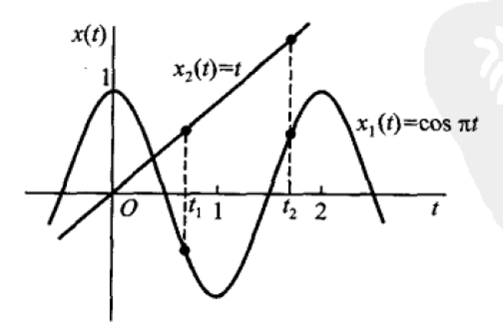
\includegraphics[scale=0.32]{sin_t}
	\column{0.6\textwidth}
	样本函数: $X(\bullet,\xi)=\{\cos\pi t, t\}, \xi\in \Omega$\\
	状态空间: $S=\{\cos\pi t_0, t_0\}, \forall t_0\in (-\infty, +\infty)$\\
	每次试验的结果是下列事件集合之一:
	\[ \{(H,T),(T,H),(H,H),(T,T)\} \]
\end{columns}
\end{frame}

\begin{frame}
\begin{example}
	考察$[0,t_0]$时间内某网站收到的访问次数$X(t_0)$, $X(t_0)$则是一个随机变量。
	\begin{itemize}
		\item 如果要长时间内该网站的访问次数,则需要让$t$变化起来,即$t$趋于无穷大,则$X(t)$是一簇随机变量.
		\item 此时$X(t)$是与时间有关系的随机变量, 称$\{X(t),t\in[0,\infty]\}$是随机过程。
	\end{itemize}
\end{example}
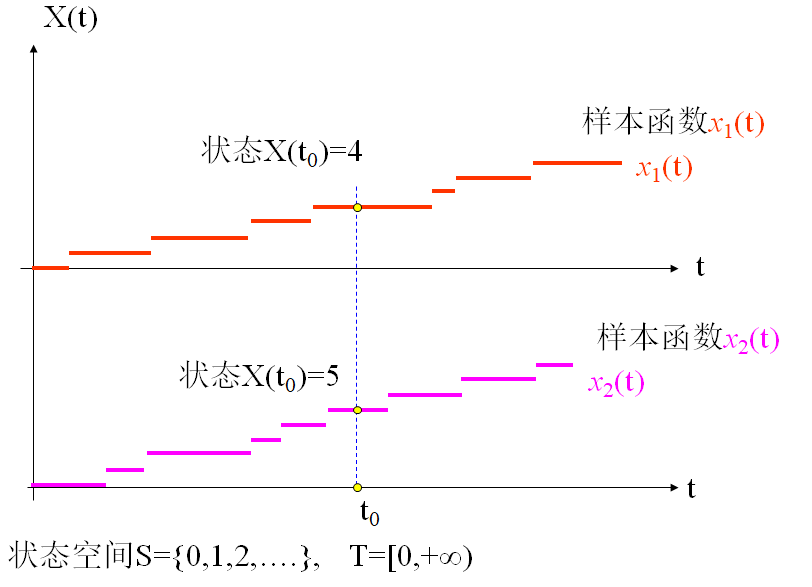
\includegraphics[scale=0.2]{sampleFun1}	
\end{frame}

\begin{frame}
\begin{example}
具有随机初位相的简谐波
\[X(t)=A\cos(\omega t+\Phi)\]
其中$A,\omega$为常数,$\Phi$服从$[0,2\pi]$上的均匀分布。
\begin{itemize}
	\item 由于初位相的随机性,在某时刻$t=t_0,X(t)$是一个随机变量.
	\item 若要观察任一时刻$t$的波形,则需要用一簇随机变量$X(t)$描述. 
	\item 称$\{X(t),t\in[0,\infty]\}$是随机过程。
\end{itemize}	
\end{example}
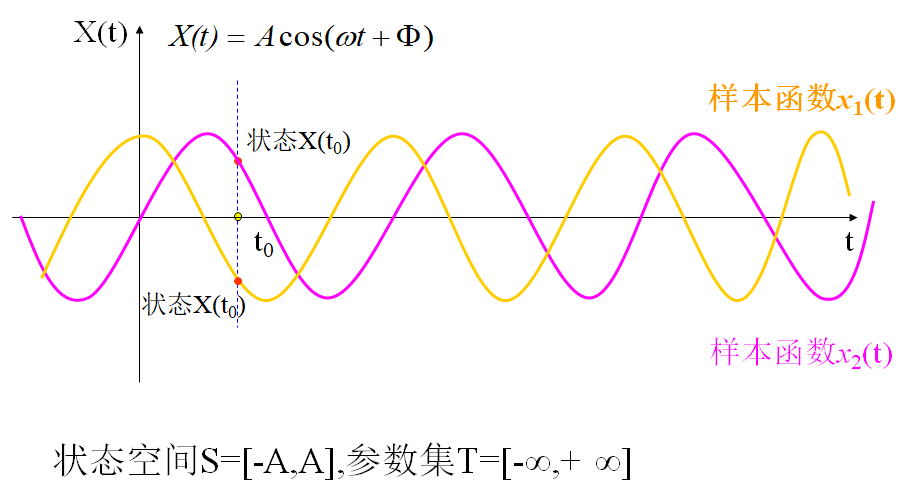
\includegraphics[scale=0.2]{sampleFun2}	
\end{frame}

\begin{frame}
\begin{columns}
\column{0.7\textwidth}
\begin{example}
三次热噪声电压测量结果:固定$t$时刻电压,对应一个随机变量$v(t)$; \\
无限个$t$,则无限个电压---时间的函数族构成一随机过程。\\
\end{example}
样本函数: $X(\bullet,\xi)=\{v_k(t)\}, k=1,2,\dots, \xi\in \Omega$\\
状态空间: $S=\{v_k(t_0)\}, k=1,2,\dots, \forall t_0\in (-\infty, +\infty)$
\column{0.3\textwidth}
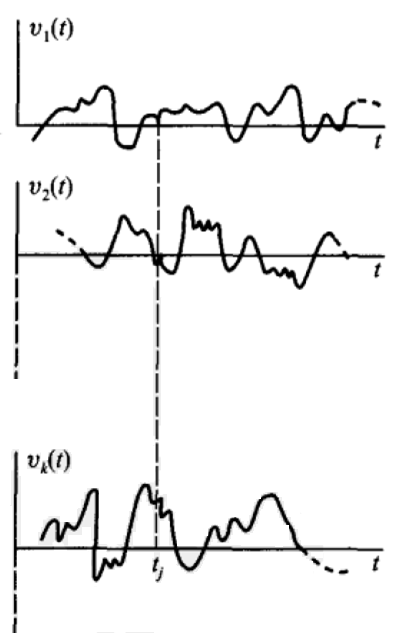
\includegraphics[scale=0.3]{vt}
\end{columns}
\end{frame}

\begin{frame}
\begin{example}
生物群体的增长问题.以$X_t$表示在时刻$t$某种生物群体的个数,则对每一个固定的$t,X_t$是一个随机变量。 
\begin{itemize}
\item 如果从$t=0$开始,每隔24小时对群体的个数观察一次,则对每一个$t$,$X_t$是一簇随机变量。记为$X_n,n=0,1,\dots$
\item 若要观察任一时刻$t$的波形,则需要用一族随机变量$X(t)$描述. 
\item 称$\{X_t,t=0,1,2,\dots\}$是随机过程。
\end{itemize}	
\end{example}
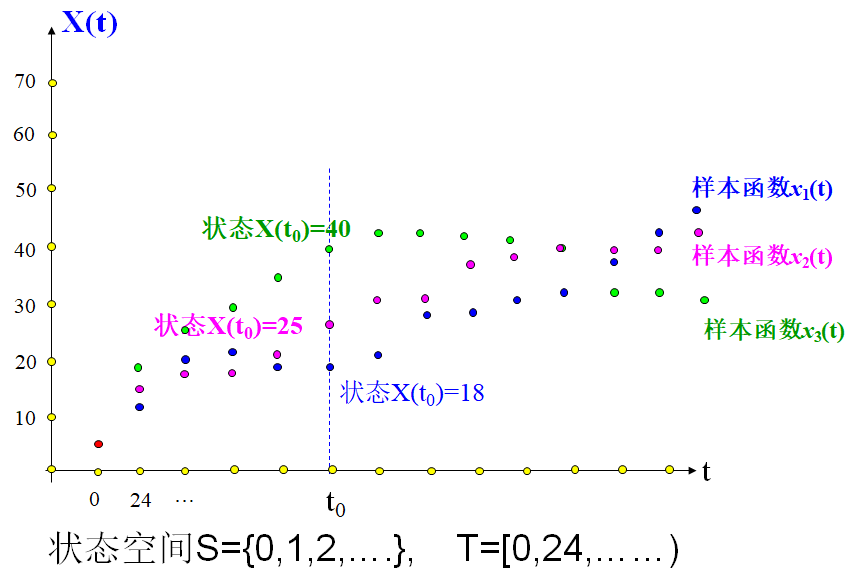
\includegraphics[scale=0.15]{sampleFun3}	
\end{frame}

\begin{frame}
\begin{example}
	设随机相位正弦信号$s(t; \theta)=a\cos(\omega_0 t+\theta)$, 其中振幅$a$和$\omega_0$为常数, 相位$\theta$是一随机变量,它服从$[-\pi,\pi]$上的均匀分布。写出$s(t;\theta)$的样本函数。
\end{example}
解: \\
当$\theta$在$[-\pi,\pi]$内任取定值时,如\\
当$\theta=0$, 则样本函数为
$$s_1(t; \theta=0)=a\cos\omega_0t$$
当$\theta=\frac{\pi}{2}$, 则样本函数为
$$s_2(t; \theta=\frac{\pi}{2})=a\cos(\omega_0t+\frac{\pi}{2})=-a\sin\omega_0t$$
\end{frame}

\section{随机过程的统计描述}

\begin{frame}{一维概率密度函数}
连续随机过程$\{X(t,\xi),t\in T,\xi\in\Omega \}$的$M$个样本函数如图。通常用\textbf{有限维概率密度函数}来描述随机过程。

\medskip
\begin{columns}
	\column{0.6\textwidth}
	\begin{block}{}
		设$\{X(t,\xi),t\in T,\xi\in\Omega \}$是一随机过程,对于任意固定的时刻$t,X(t,\xi)$是一随机变量,称
		\[F(x;t)=P\{X(t,\xi)\le x\},x\in\mathbb{R},t\in T \]
		为该随机过程的\textbf{一维累积分布函数}。\\
		如果$F(x;t)$对$x$的一阶导数存在,则有
		\[p(x;t)=\frac{dF(x;t)}{dx}\]
		$p(x;t)$称为随机过程$X(t,\xi)$的\textbf{一维概率密度函数}。
	\end{block}
	\column{0.3\textwidth}
	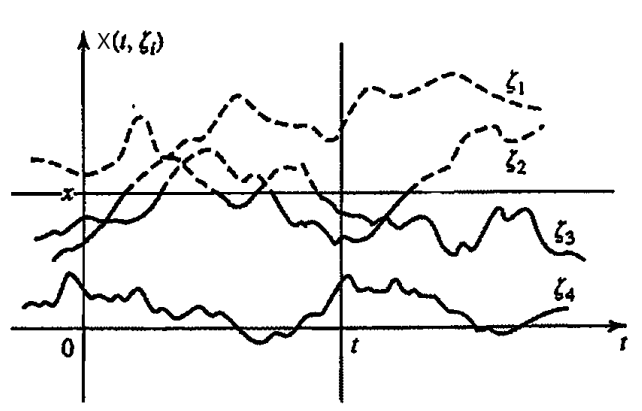
\includegraphics[scale=0.25]{sampleFun4}
\end{columns}
\end{frame}

\begin{frame}{二维联合概率密度函数}
对于任意固定的时刻$t_1,t_2\in T$, 随机变量$X(t_1,\xi),X(t_2,\xi)$构成二维矢量$[X(t_1,\xi),X(t_2,\xi)]^T$,称
\[F(x_1,x_2;t_1,t_2)=P\{X(t_1,\xi)\le x_1,X(t_2,\xi)\le x_2\},x_1,x_2\in\mathbb{R},t_1,t_2\in T \]
为该随机过程的\textbf{二维累积分布函数}。\\
如果$F(x_1,x_2;t_1,t_2)\in T$对$x_1,x_2$的二阶混合偏导数存在,则有
\[p(x_1,x_2;t_1,t_2)=\frac{\partial^2 F(x_1,x_2;t_1,t_2)}{\partial x_1\partial x_2}\]
$p(x;t)$称为随机过程$X(t,\xi)$的\textbf{二维联合概率密度函数}。
\end{frame}

\begin{frame}{N维联合概率密度函数}
推广至N维随机矢量的情况\\
随机过程的\textbf{N维累积分布函数}
\begin{align*}
F(x_1,x_2,\cdots,x_N;t_1,t_2,\cdots,t_N)&=\\
&P\{X(t_1,\xi)\le x_1,X(t_2,\xi),\cdots,X(t_N,\xi)\le x_N\},&\\
&x_1,x_2,\cdots,x_N\in\mathbb{R},t_1,t_2,\cdots,t_N\in T
\end{align*}
随机过程的\textbf{N维联合概率密度函数}
\begin{align*}
p(x_1,x_2,\cdots,x_N;t_1,t_2,\cdots,t_N)&=\\
&\frac{\partial^N F(x_1,x_2,\cdots,x_N;t_1,t_2,\cdots,t_N)}{\partial x_1\partial x_2\cdots\partial x_N}
\end{align*}
\end{frame}

\begin{frame}{一维雅可比变换法}
设一维随机变量为$X(\xi)$,它的概率密度函数为$p(x)$已知,若$X(\xi)$的一个函数为
\[Y(\xi)=g(X(\xi)) \]
该函数也是一维随机变量。若它的反函数存在,即有
\[X(\xi)=h(Y(\xi)) \]
且连续可导,则$Y(\xi)$的概率密度函数为
\[p(y)=p[x=h(y)]|J| \]
这种变换称为\textbf{一维雅可比变换},其中\textbf{雅可比}$J=\frac{dh(Y)}{dY}$, $|\bullet|$是绝对值符号。
\begin{block}{Notes}
	$Y(\xi)$的概率密度函数$p(y)$可以通过它的反函数$X(\xi)$的概率密度函数$p(x)$与雅可比的乘积得到。进而, $E(Y)=E[g(X)]=\int_{-\infty}^{\infty}g(x)p(x)dx$。
\end{block}
\end{frame}

\begin{frame}
\begin{example}
	设随机过程$X(t)=V\cos\omega t,t\in(-\infty,+\infty)$, 其中$\omega$为常数, $V$服从$[0,1]$上的均匀分布。
	\begin{enumerate}
		\item 确定$\{X(t),t\in(-\infty,+\infty)\}$的两个样本函数。
		\item 求$t=0,t=3\pi/4\omega$时,随机变量$X(t)$的概率密度函数。
		\item 求$t=\pi/2\omega$时, $X(t)$的分布函数。
	\end{enumerate}
\end{example}
\end{frame}

\begin{frame}
解:
\begin{enumerate}
	\item $V$服从$[0,1]$上的均匀分布, 取$V=1/2,1/3$分别得到两个样本函数
	\[X_1(t)=\frac{1}{2}\cos\omega t,X_2(t)=\frac{1}{3}\cos\omega t\]
	\item $t=0$时, $x(t)=V\cos\omega 0=V$,而$V$为$[0,1]$上的均匀分布,则
	$$
	p(x;t=0)=\begin{cases}
	1 & 0\le x\le 1\\
	0 &\text{其它}
	
\end{cases}
$$
\end{enumerate}
\end{frame}

\begin{frame}
解(续):
\begin{enumerate}
	\setcounter{enumi}{1} %设定起始编号 
	\item (续) 当$t=\frac{3\pi}{4\omega}$时,$X(t)=V\cos\omega\frac{3\pi}{4\omega}=-\frac{\sqrt{2}}{2}V$\\
	由于函数$x=-\frac{\sqrt{2}}{2}V$的反函数为$V=h(x)=-\sqrt{2}x$,其导数为$h^\prime(x)=-\sqrt{2}$,则利用一维雅可比变换公式,求得
	\begin{align*}
		p(x,t=\frac{3\pi}{4\omega}) &=\begin{cases}
		p_V(h(x))|h^\prime(x)| &0\le h(x)\le 1\\
		0 &\text{其它}
		\end{cases}\\
		&=\begin{cases}
		\sqrt{2} &0\le -\sqrt{2}x\le 1\\
		0 &\text{其它}
		\end{cases}\\
		&=\begin{cases}
		\sqrt{2} &\frac{-\sqrt{2}}{2}\le x\le 0\\
		0 &\text{其它}
		\end{cases}
	\end{align*}
\end{enumerate}
\end{frame}

\begin{frame}
解(续):
\begin{enumerate}
	\setcounter{enumi}{2} %设定起始编号 
	\item $t=\frac{\pi}{2\omega}$时,$X(t)=V\cos\omega\frac{pi}{2\omega}=0$, 此时$X(t=\frac{\pi}{2\omega})$是单点分布,则
	\begin{align*}
	F(x,t=\frac{\pi}{2\omega}) &=P\{X(t)\le x \}\\
	&=\begin{cases}
	1 &x\ge 0\\
	0 &x<0
	\end{cases}
	\end{align*}
\end{enumerate}
\end{frame}

\begin{frame}
\begin{example}
设有一采用脉宽调制以传输信息的通信系统。脉冲的重复周期为$T$,每个周期传输一个值, 脉冲宽度收到随机信息的调制,使每个脉冲的宽度$\tau$服从$(0,T)$上的均匀分布,而且不同周期的脉宽是相互统计独立的随机变量。脉冲的幅度为常数$A$。 也就是说,这个通信系统传送的信号是随机脉宽等幅度的周期信号,它是一个随机过程。下图画出了它的一个样本函数。试求该随机过程$x(t)$的一维概率密度函数。
\begin{figure}
	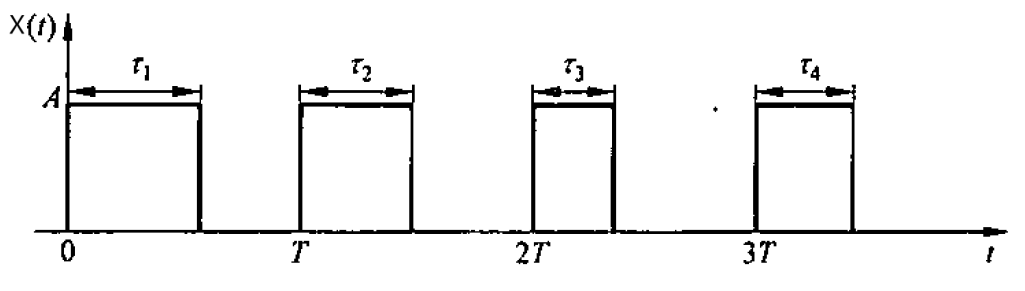
\includegraphics[scale=0.3]{2_10SampleFun}
	\caption {脉宽调制信号的一个样本函数}
\end{figure}
\end{example}
\end{frame}

\begin{frame}[shrink]
\begin{example}[解]
	因为脉冲的重复周期为$T$,所以只需求出一个周期的概率密度函数。\\
	在一个周期内,随机信号为
	\[
	x(t)=\begin{cases}
	A,&0\le t\le\tau\\
	0,&\tau<t\le T
	\end{cases} 
	\]
	$x(t)$的分布函数为
	\[
	F(x;t)=\begin{cases}
	0,&x<0\\
	\frac{t}{T},&0\le x<A\\
	1,&x\ge A
	\end{cases} 
	\]
	所以,它的一维概率密度函数为:
	\[p(x;t)=\frac{t}{T}\delta(x)+(1-\frac{t}{T})\delta(x-A) \]
\end{example}
\small
由$\delta$函数性质, 当$x=0$时, $\delta(x)=\infty$; 其它, $\delta(x)=0$. 并且$\int_{-\infty}^{\infty}\delta(x)dx=1$\\
可以验证以上分布函数的正确性.  $F(x; t)=P\{x(t)\le x\}=\int_{-\infty}^{x}p(u)du$
\end{frame}

%\section{随机过程的统计平均量}

\begin{frame}
函数的均值
\[\bar{y}=\frac{1}{b-a}\lim\limits_{\Delta x\to 0}\sum\limits_{i=1}^{n}f(x_{i-1})\Delta x=\frac{1}{b-a}\int_{a}^{b}f(x)dx \]
交流电$i=I_m\sin\omega t$,\\
电压$u=iR=I_mR\sin\omega t$,\\
功率$p=ui=I_m^2R\sin^2\omega t$\\
此功率在长度为一个周期的区间$[0,\frac{2\pi}{\omega}]$上的平均值
\[\bar{p}=\frac{1}{\frac{2\pi}{\omega}}\int_{0}^{\frac{2\pi}{\omega}}I_m^2R\sin^2\omega tdt=\frac{I_m^2R}{2}=\frac{I_mU_m}{2},(U_m=I_mR) \]
$I_m,U_m$为交流电电流、电压的最大值,$\omega$为交流电的角频率。
\end{frame}

\begin{frame}
\begin{block}{随机过程的均值$\mu_x(t)$: 表示随机过程在$t$时刻状态取值的理论平均值}
	\[\mu_x(t)\mathop{=}^{def}E[x(t)]=\int_{-\infty}^{\infty}xp(x;t)dx \]
	如果$x(t)$是电压或电流,则$\mu_x(t)$可以理解为在$t$时刻的``直流分量''。
\end{block}

\begin{block}{随机过程的均方值$\varphi_x^2(t)$}
	\[\varphi_x^2(t)\mathop{=}^{def}E[x^2(t)]=\int_{-\infty}^{\infty}x^2p(x;t)dx \]
	如果$X(t)$是电压或电流,则$\varphi_x^2(t)$可以理解在$t$时刻它在$1\Omega$电阻上消耗的``平均功率''。
\end{block}
\end{frame}

\begin{frame}
\begin{block}{随机过程的方差/标准偏差$\delta_x^2(t)$}
\[\sigma_x^2(t)\mathop{=}^{def}E[(x(t)-\mu_x(t))^2]=\int_{-\infty}^{\infty}(x-\mu_x(t))^2p(x;t)dx \]
方差$\sigma_x^2(t)$表示随机过程在$t$时刻取其值\textbf{偏离其均值}$\mu_x(t)$的离散程度。\\
如果$x(t)$是电压或电流,则$\delta_x^2(t)$可以理解在$t$时刻它在$1\Omega$电阻上消耗的``交流功率''。
\end{block}
\begin{block}{均值$\mu_x(t)$,均方值$\varphi_x^2(t)$,方差$\delta_x^2(t)$之间的关系}
\[\sigma_x^2(t)=\varphi_x^2(t)-\mu_x^2(t)\]
\end{block}
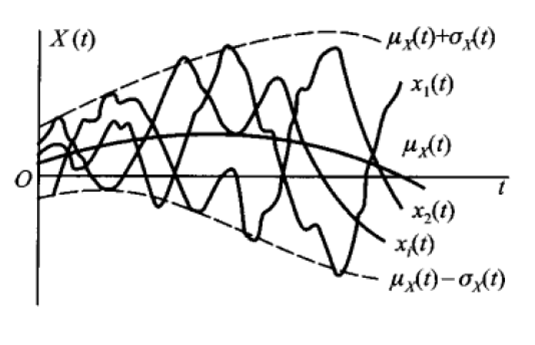
\includegraphics[scale=0.4]{delta}
\end{frame}

\begin{frame}{均匀分布随机变量$x$的均值$\mu_x$和方差$\sigma_x^2$}
\begin{example}
	求如图均匀分布随机变量$x$的均值$\mu_x$和方差$\sigma_x^2$。
	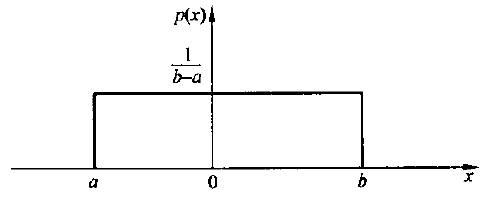
\includegraphics[scale=0.3]{ex2-1}
\end{example}
\end{frame}

\begin{frame}{均匀分布随机变量$x$的均值$\mu_x$和方差$\sigma_x^2$}
解: 随机变量$x$的概率密度函数$p(x)$为
\[p(x)=\begin{cases}
\frac{1}{b-a}, &a\le x\le b\\
0, &\text{其他}
\end{cases} \]

根据随机变量均值的定义,有
\begin{align*}
\mu_x=E(x)&=\int_{-\infty}^{\infty}xp(x)dx=\int_{a}^{b}\frac{1}{b-a}xdx =\frac{a+b}{2}
\end{align*}
根据随机变量方差的定义,有
\begin{align*}
\sigma_x^2=E[(x-\mu_x)^2]&=\int_{-\infty}^{\infty}(x-\mu_x)^2p(x)dx=\int_{a}^{b}\left(x-\frac{a+b}{2}\right)^2\frac{1}{b-a}dx \\
&=\frac{(b-a)^2}{12}
\end{align*}	
\end{frame}

\begin{frame}
\begin{block}{随机过程的自相关函数$r_x(t_j,t_k)$}
\begin{align*}
r_x(t_j,t_k)&\mathop{=}^{def}E[x(t_j)x(t_k)]\\
&=\int_{-\infty}^{\infty}	\int_{-\infty}^{\infty}x_jx_kp(x_j,x_k;t_j,t_k)dx_jdx_k
\end{align*}
\end{block}
随机过程的自相关函数$r_x(t_j,t_k)$可以理解为它的两个随机变量$x(t_j)$与$x(t_k)$之间\textbf{含有均值}时的相关程度的度量。显然
\[r_x(t,t)=\varphi_x^2(t)\]
\end{frame}

\begin{frame}
\begin{example}
	设随机过程$x(t)$的均值为$\mu_x(t)$,自相关函数为$r_x(t_j,t_k)$。若有随机过程$y(t)=a(t)x(t)+b(t)$, 其中$a(t),b(t)$是确知函数。求随机过程$y(t)$的均值和自相关函数。
\end{example}
\end{frame}

\begin{frame}
解:\\
由均值定义$E[x(\xi)]\mathop{=}\limits^{def}\mu_x=\int_{-\infty}^{\infty}xp(x)dx$知:\\
确知函数$a(t)$的均值:
\begin{align*}
E[a(t)]&=\int_{-\infty}^{\infty}a(t)p(x)dx\\
&=a(t)\int_{-\infty}^{\infty}p(x)dx &&\text{by $a(t)$是常数}\\
&=a(t)\cdot 1 &&by \int_{-\infty}^{\infty}p(x)dx=1\\
&=a(t)
\end{align*}
\textcolor{blue}{结论: 确知函数$a(t)$的均值$E[a(t)]=a(t)$}
\end{frame}

\begin{frame}
解(续):随机过程$y(t)$的均值为:
\begin{align*}
\mu_y&=E[y(t)]=E[a(t)x(t)+b(t)]=E[a(t)x(t)]+E[b(t)]\\
&=a(t)E[x(t)]+b(t)=a(t)\mu_x+b(t)
\end{align*}
随机过程$y(t)$的自相关函数为:
\begin{align*}
r_y(t_j,t_k)&=E[y(t_j)y(t_k)]\\
&=E[(a(t_j)x(t_j)+b(t_j))(a(t_k)x(t_k)+b(t_k))]\\
&=a(t_j)a(t_k)E[x(t_j)x(t_k)]+a(t_j)b(t_k)E[x(t_j)]\\
&+b(t_j)a(t_k)E[x(t_k)]+b(t_j)b(t_k)\\
&=a(t_j)a(t_k)r_x(t_j,t_k)+a(t_j)b(t_k)\mu_x(t_j)+b(t_j)a(t_k)\mu_x(t_k)+b(t_j)b(t_k)
\end{align*}
其中: $,r_x(t_j,t_k)=E[x(t_j)x(t_k)],\mu_x(t_j)=E[x(t_j)], \mu_x(t_k)=E[x(t_k)]$
\end{frame}

\begin{frame}
\begin{example}
	设随机相位正弦信号$s(t; \theta)=a\cos(\omega_0 t+\theta)$, 其中振幅$a$和$\omega_0$为常数, 相位$\theta$是一随机变量,它服从$[-\pi,\pi]$上的均匀分布。
	\begin{enumerate}
		\item 求该过程的均值$E[s(t; \theta)]$
		\item 自相关函数$E[s(t_j; \theta)s(t_k; \theta)]$。
	\end{enumerate}
\end{example}
\end{frame}

\begin{frame}
解:
\begin{enumerate}
\item 因为相位$\theta$服从$[-\pi,\pi]$上的均匀分布,所以,
$$p(\theta)=\begin{cases}
\frac{1}{2\pi}, & -\pi\le\theta\le\pi\\
0, &\text{其它}
\end{cases} $$ 
该随机过程的均值为:
\begin{align*}
\mu_{x}(t)&=E[s(t; \theta)]=E[a\cos(\omega_0t+\theta)]\\
&=\int_{-\infty}^{\infty}a\cos(\omega_0t+\theta)p(\theta)d\theta\\
&=\int_{-\pi}^{\pi}a\cos(\omega_0t+\theta)\frac{1}{2\pi}d\theta\\
&=\frac{a}{2\pi}\int_{-\pi}^{\pi}\cos(\omega_0t+\theta)d\theta\\
&=0
\end{align*}
\end{enumerate}
\end{frame}

\begin{frame}
解(续): \footnote{$\cos A\cos B=\frac{1}{2}\cos (A+B)\cos(A-B)$}
\begin{enumerate}
\setcounter{enumi}{1} %设定起始编号 
\item 该随机过程的自相关函数为:
\begin{align*}
r_x(t_j,t_k)&=E[s(t_j)s(t_k)]\\
&=\int_{-\infty}^{\infty}a\cos(\omega_0t_j+\theta)a\cos(\omega_0t_k+\theta)p(\theta)d\theta\\
&=\frac{a^2}{4\pi}\int_{-\pi}^{\pi}[\cos(\omega_0t_j+\omega_0t_k+2\theta)+\cos\omega_0(t_k-t_j)]d\theta\\
&=\frac{a^2}{2}\cos\omega_0\tau,\qquad(\tau=t_k-t_j)
\end{align*}
\end{enumerate}
\end{frame}

\begin{frame}
\begin{block}{随机过程的自协方差函数$c_x(t_j,t_k)$}
\begin{align*}
c_x(t_j,t_k)&\mathop{=}^{def}E[((x(t_j)-\mu_x(t_j)(x(t_k)-\mu_x(t_k)]\\
&=\int_{-\infty}^{\infty}\int_{-\infty}^{\infty}(x_j-\mu_x(t_j))(x_k-\mu_x(t_k))p(x_j,x_k;t_j,t_k)dx_idx_k
\end{align*}
\end{block}
随机过程的自协方差函数$c_x(t_j,t_k)$可以理解为它的两个随机变量$x(t_j)$与$x(t_k)$之间的相关程度的度量。\\
而随机过程的自相关函数$r_x(t_j,t_k)$可以理解为它的两个随机变量$x(t_j)$与$x(t_k)$之间\textbf{含有均值}时的相关程度的度量。\\
它们的自相关系数定义为
\[\rho_x(t_j,t_k)\mathop{=}^{def}\frac{c_x(t_j,t_k)}{\sigma_x(t_j)\sigma_x(t_k)}\]
易证
\[c_x(t_j,t_k)=r_x(t_j,t_k)-\mu_x(t_j)\mu_x(t_k),\quad c_x(t,t)=\sigma_x^2(t)\]
\end{frame}

\begin{frame}{随机过程的统计平均量之间的关系}
\begin{itemize}
	\item 随机过程的均值$\mu_x(t)$: 表示随机过程在$t$时刻状态取值的\textbf{理论平均值}。
	\item 方差$\sigma_x^2(t)$表示随机过程在$t$时刻取其值\textbf{偏离其均值}$\mu_x(t)$的离散程度。
	\item 随机过程的自相关函数$r_x(t_j,t_k)$可以理解为它的两个随机变量$x(t_j)$与$x(t_k)$之间\textbf{含有均值}时的相关程度的度量。
	\item 随机过程的自协方差函数$c_x(t_j,t_k)$
	随机过程的自协方差函数$c_x(t_j,t_k)$可以理解为它的两个随机变量$x(t_j)$与$x(t_k)$之间的相关程度的度量。
\end{itemize}
\[c_x(t_j,t_k)=r_x(t_j,t_k)-\mu_x(t_j)\mu_x(t_k),\quad c_x(t,t)=\sigma_x^2(t)\]
\begin{columns}
	\column{0.6\textwidth}
	均值$\mu_x(t)$,均方值$\varphi_x^2(t)$,方差$\delta_x^2(t)$之间的关系:
	\[\sigma_x^2(t)=\varphi_x^2(t)-\mu_x^2(t)\]
	\column{0.3\textwidth}
	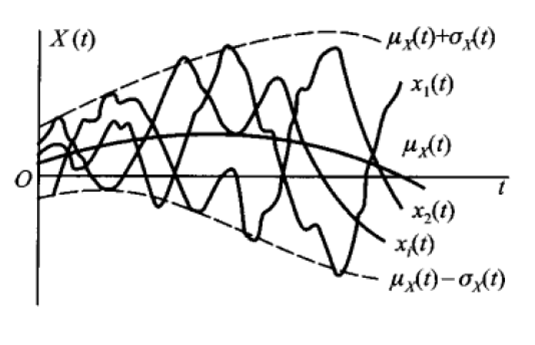
\includegraphics[scale=0.4]{delta}
\end{columns}
\end{frame}

\begin{frame}
\begin{block}{随机过程的互相关函数$r_{xy}(t_j,t_k)$}
对于两个随机过程$x(t)$和$y(t)$, 其互相关函数定义为
\begin{align*}
r_{xy}(t_j,t_k) &\mathop{=}^{def}E[x(t_j)y(t_k)]\\
&=\int_{-\infty}^{\infty}\int_{-\infty}^{\infty}x_jy_kp(x_j,t_j;y_k,t_k)dx_jdy_k
\end{align*}
式中, $p(x_j,t_j;y_k,t_k)$是$x(t)$与$y(t)$的二维混合概率密度函数。
\end{block}
\end{frame}

\begin{frame}
\begin{block}{随机过程的互协方差函数$c_{xy}(t_j,t_k)$}
\begin{align*}
c_{xy}(t_j,t_k)&\mathop{=}^{def}E[(x(t_j)-\mu_x(t_j))(y(t_k)-\mu_x(t_k))]\\
&=\int_{-\infty}^{\infty}\int_{-\infty}^{\infty}(x_j-\mu_x(t_j))(y_k-\mu_x(t_k))p(x_j,t_j;x_k,t_k)dx_jdy_k
\end{align*}
\end{block}
随机过程$x(t)$和$y(t)$的互协方差函数$c_{xy}(t_j,t_k)$可以理解为它们各自的随机变量$x(t_j)$与$y(t_k)$之间的相关程度, 实际上表示两个随机过程$x(t)$与$y(t)$之间的相关程度。它们的互相关系数定义为
\[\rho_{xy}(t_j,t_k)\mathop{=}^{def}\frac{c_{xy}(t_j,t_k)}{\sigma_x(t_j)\sigma_x(t_k)}\]
易证
\[c_{xy}(t_j,t_k)=r_{xy}(t_j,t_k)-\mu_x(t_j)\mu_y(t_k)\]
\end{frame}

\section{随机过程的平稳性}

\begin{frame}
\begin{definition}[广义平稳随机过程,简称平稳随机过程]
随机过程$x(t)$的平均统计量满足
\begin{enumerate}
\item $x(t)$的均值是与时间$t$无关的常数,即
\[E[x(t)]=\mu_x\]
\item $x(t)$的自相关函数只取决于时间间隔$\tau=t_k-t_j$,而与时间的起始时刻无关,即
\[E[x(t_j)x(t_k)]=E[x(t_j)x(t_j+\tau)]=r_x(\tau) \]
\end{enumerate}
\end{definition}
平稳随机过程$x(t)$自相关函数$r_x(t_k-t_j)$仅取决于时间间隔$(t_k-t_j)$,而与时间的起始时刻无关。$E[x(t_j)x(t_k)]=r_x[t_k-t_j]$
\end{frame}

\begin{frame}{平稳随机过程的统计平均量之间的关系}
平稳随机过程x(t)的均值$\mu_x$, 均方值$\varphi_x^2$, 方差$\sigma_x^2$,自相关函数$r_x(\tau)$,自协方差函数$c_x(\tau)$之间的关系
\begin{align*}
&\sigma_x^2=\varphi_x^2-\mu_x^2\\
&r_x(\tau)=r_x(-\tau)\\
&c_x(\tau)=r_x(\tau)-\mu_x^2\\
&c_x(\tau)=c_x(-\tau)\\
&\varphi_x^2=r_x(0)\\
&\sigma_x^2=c_x(0)\\
&r_x(0)\ge|r_x(\tau)|, \tau\ne 0\\
&c_x(0)\ge|c_x(\tau)|, \tau\ne 0
\end{align*}
\end{frame}

\begin{frame}[shrink]
\begin{example}
	假定平稳随机过程$x(t)$是周期的, 周期为$T$, 即
	\[x(t)=x(t+T) \]
	证明其自相关函数$r_x(\tau)$也是以$T$为周期的, 即
	\[r_x(\tau)=r_x(\tau+T) \]
\end{example}
\begin{proof}
	因为
	\begin{align*}
	r_x(\tau)&=E[x(t)x(t+\tau)]\\
	&=E[x(t)x(t+\tau+T)]&& \text{by } x(t+\tau)=x(t+\tau+T)\\
	&=r_x(\tau+T)
	\end{align*}
	所以, 自相关函数$r_x(\tau)$也是以$T$为周期的。
\end{proof}
\end{frame}

\begin{frame}
\begin{definition}[联合平稳随机过程]
设$x(t)$和$y(t)$分别是两个平稳的随机过程, 如果对于任意的$\Delta t$, 有$r_{xy}(t_j+\Delta t,t_k+\Delta t)=r_{xy}(t_j,t_k)$, 即互相关函数$r_{xy}(t_j,t_k)=r_{xy}(\tau),(\tau=t_k-t_j)$仅与时间间隔$\tau$有关,而与$t_j$和$t_k$无关,则称过程$x(t)$与$y(t)$是联合平稳的随机过程。
\end{definition}
\begin{block}{联合平稳随机过程$x(t)$与$y(t)$的互协方差函数}
\[c_{xy}(t_j,t_k)=c_{xy}(\tau)=r_{xy}(\tau)-\mu_x\mu_y, \tau=t_k-t_j\]
互相关系数:
\[\rho_{xy}(\tau)\mathop{=}^{def}=\frac{c_{xy}(t_j,t_k)}{\sigma_x(t_j)\sigma_y(t_k)}=\frac{c_{xy}(\tau)}{\sigma_x\sigma_y}\]
\begin{align*}
r_{xy}(\tau)&=r_{yx}(-\tau)\\
c_{xy}(\tau)&=c_{yx}(-\tau)
\end{align*}
\end{block}
\end{frame}

\section{随机过程的正交性、不相关性和统计独立性}

\begin{frame}{$x(t)$的正交性与互不相关性}
随机过程$x(t)$的任意两个不同时刻的随机变量$x(t_j)$与$x(t_k)$之间是否相互正交、互不相关和相关统计独立,表征了随机过程的重要统计特性。
\begin{definition}
	设$x(t_j),x(t_k)$是随机过程$x(t)$的任意两个不同时刻的随机变量,其均值分别为$\mu_x(t_j)$和$\mu_x(t_k)$,自相关函数为$r_x(t_j,t_k)$,自协方差函数为$c_x(t_j,t_k)$。
	\begin{enumerate}
		\item 相互正交
		$$r_x(t_j,t_k)\mathop{=}^{def}E[x(t_j)x(t_k)]=0, \quad j\ne k$$
		\item 互不相关
		$$c_x(t_j,t_k)\mathop{=}^{def}E[((x(t_j)-\mu_x(t_j)(x(t_k)-\mu_x(t_k)]=0, \quad j\ne k$$
		\item 互不相关的等价条件
		$$c_x(t_j,t_k)=r_x(t_j,t_k)-\mu_x(t_j)\mu_x(t_k), j\ne k \implies r_x(t_j,t_k)=\mu_x(t_j)\mu_x(t_k),j\ne k $$
	\end{enumerate}
	
\end{definition}
\end{frame}

\begin{frame}{平稳随机过程$x(t)$的正交性与互相关性}
\begin{definition}[]
如果$x(t)$是平稳随机过程,
\begin{enumerate}
	\item 相互正交:
	\[r_x(\tau)=0,\tau=t_k-t_j\]
	\item 互不相关:
	\[c_x(\tau)=0,\tau=t_k-t_j\]
	\item
	互不相关的等价条件
	\[r_x(\tau)=\mu_x^2,\tau=t_k-t_j\]
\end{enumerate}
\end{definition}
\end{frame}

\begin{frame}{$x(t)$的统计独立性}
\begin{definition}[]
设$x(t_1),x(t_2),\dots,x(t_N)$是随机过程$x(t)$在不同时刻$t_k(k=1,2,\dots,t_N)$的随机变量, 如果其N维联合概率密度函数对于任意的$N\ge 1$和所有时刻$t_k(k=1,2,\dots,N)$都能够表示成各自一维概率密度函数之积的形式,即
\begin{align*}
p(x_1,x_2,\dots,x_N; t_1,t_2,\dots,t_N)\\
=p(x_1;t_1)p(x_2;t_2)\cdots p(x_N;t_N)
\end{align*}
则称$x(t)$是相互统计独立的随机变量过程。
\end{definition}
\end{frame}

\begin{frame}{$x(t)$的正交性,不相关性以及统计独立性之间的关系}
\begin{enumerate}
\item 均值$\mu_x(t_j)=0,\mu_x(t_k)=0$则, $x(t)$相互正交$\Leftrightarrow$互不相关\\
\item $x(t)$相互统计独立$\Rightarrow$互不相关
\item $x(t)$互不相关$\nRightarrow$相互统计独立。但是若$x(t)$服从联合高斯分布,则互不相关$\Leftrightarrow$相互统计独立
\end{enumerate}
第1条可由$x(t)$互不相关的等价条件$r_x(t_j,t_k)=\mu_x(t_j)\mu_x(t_k),j\ne k $直接导出。
现证明第2条,第3条的证明见后。
\end{frame}

\begin{frame}
证明:如果$x(t)$是一个相互统计独立随机变量过程,则它一定是一个互不相关随机变量过程。
\begin{proof}%[caption]
	设$x(t_j)$与$x(t_k)$是相互统计独立的, 则其自相关函数为
	\begin{align*}
	r_x(t_j,t_k)&\mathop{=}^{def}E[x(t_j)x(t_k)]\\
	&=\int_{-\infty}^{\infty}\int_{-\infty}^{\infty}x_jx_kp(x_j,x_k;t_j,t_k)dx_jd_k\\
	&=\int_{-\infty}^{\infty}x_jp(x_j;t_j)dx_j\int_{-\infty}^{\infty}x_jp(x_k;t_k)dx_k\\
	&=\mu_x(t_j)\mu_x(t_k)
	\end{align*}
	这正是$x(t)$互不相关的等价条件$r_x(t_j,t_k)=\mu_x(t_j)\mu_x(t_k),j\ne k $,所以$x(t)$统计独立$\implies$ 互不相关
\end{proof}
由证明过程,可以得到: \textcolor{blue}{$x(t)$相互统计独立,则,$E[x(t_j)x(t_k)]=E[x(t_j)]E[x(t_k)]$}
\end{frame}

\begin{frame}{两个随机过程$x(t), y(t)$的正交性与互不相关性}
设$x(t_j)$是$x(t)$在$t_j$时刻的随机变量, $y(t_k)$是$y(t)$在$t_k$时刻的随机变量。
\begin{definition}
	$x(t)$在$t_j$, $y(t)$在$t_k$的均值分别为$\mu_x(t_j)$和$\mu_y(t_k)$, 互相关函数为$r_{xy}(t_j,t_k)$, 互协方差函数为$c_{xy}(t_j,t_k)$。
	\begin{enumerate}
		\item 相互正交
		$$r_{xy}(t_j,t_k)\mathop{=}^{def}E[x(t_j)y(t_k)]=0, \quad j\ne k$$
		\item 互不相关
		$$c_{xy}(t_j,t_k)\mathop{=}^{def}E[((x(t_j)-\mu_x(t_j)(y(t_k)-\mu_y(t_k)]=0, \quad j\ne k$$
		\item 互不相关的等价条件
		$$c_{xy}(t_j,t_k)=r_{xy}(t_j,t_k)-\mu_x(t_j)\mu_y(t_k), j\ne k \implies r_{xy}(t_j,t_k)=\mu_x(t_j)\mu_y(t_k),j\ne k $$
	\end{enumerate}	
\end{definition}
\end{frame}

\begin{frame}{两个平稳随机过程$x(t), y(t)$的正交性与互相关性}
\begin{definition}[]
	如果$x(t), y(t)$是联合平稳的随机过程,
	\begin{enumerate}
		\item 相互正交:
		\[r_{xy}(\tau)=0,\tau=t_k-t_j\]
		\item 互不相关:
		\[c_{xy}(\tau)=0,\tau=t_k-t_j\]
		\item
		互不相关的等价条件
		\[r_{xy}(\tau)=\mu_x\mu_y,\tau=t_k-t_j\]
	\end{enumerate}
\end{definition}
\end{frame}

\begin{frame}{两个随机过程$x(t), y(t)$的统计独立性}
\begin{definition}
	如果随机过程$x(t)$和$y(t)$对任意的$N\ge 1, M\ge 1$和所有时刻$t_k(k=1,2,\dots,t_N)$与$t_k^\prime(k=1,2,\dots,M)$, 其$N+M$维联合概率密度表示为
	\begin{align*}
	p(x_1,x_2,\dots,x_N; t_1,t_2,\dots,t_N; y_1,y_2,\dots,y_N; t_1^\prime,t_2^\prime,\dots,t_M^\prime)\\
	=p(x_1,x_2,\dots,x_N; t_1,t_2,\dots,t_N)p(y_1,y_2,\dots,y_N; t_1^\prime,t_2^\prime,\dots,t_M^\prime)
	\end{align*}
	则称$x(t)$与$y(t)$是相互统计独立的两个随机变量过程。
\end{definition}
\end{frame}

\begin{frame}{相互独立的随机过程$E[x(t)y(t)]=E[x(t)]E[y(t)]$}
\begin{block}{}
	设$x(t), y(t)$是相互独立的随机过程, 则有
	\[ E[x(t)y(t)]=E[x(t)]E[y(t)]\]
	这一性质可以推广至任一两个有限个相互独立的随机变量之积的情况。
\end{block}
\begin{proof}
	\begin{align*}
	E[x(t)y(t)]&=\int_{-\infty}^{\infty}\int_{-\infty}^{\infty}xyp(x,y)dxdy\\
	&=\int_{-\infty}^{\infty}\int_{-\infty}^{\infty}xyp_x(x)p_ydxdy\\
	&=\left[\int_{-\infty}^{\infty}xp_x(x)dx\right]\left[\int_{-\infty}^{\infty}yp_y(y)dy\right]\\
	&=E[x(t)]E[y(t)]
	\end{align*}
\end{proof}
\end{frame}

\begin{frame}{$x(t),y(t)$的正交性,不相关性以及统计独立性之间的关系}
\begin{enumerate}
	\item 均值之一或同时为零, 则$x(t), y(t)$相互正交$\Leftrightarrow$互不相关\\
	\item $x(t), y(t)$相互统计独立$\Rightarrow$互不相关
	\item $x(t), y(t)$互不相关$\nRightarrow$相互统计独立。但是若$x(t), y(t)$服从联合高斯分布,则互不相关$\Leftrightarrow$相互统计独立
\end{enumerate}
\end{frame}

\begin{frame}{雷达回波信号}
\begin{example}
	设$s(t)$是雷达的发射信号, 遇到目标后的反射信号为$as(t-t_0), t_0$是信号返回的延迟时间。如果回波信号中伴有加性噪声$n(t)$, 则接收到的信号为
	\[x(t)=as(t-t_0)+n(t) \]
	\begin{enumerate}
		\item 假定$s(t)$和$n(t)$是平稳相关的, 试求互相关函数$r_{sx}(\tau)$。
		\item 如果噪声$n(t)$的均值为零, 且与$s(t)$相互统计独立, 试求互相关函数$r_{sx}(\tau)$。
	\end{enumerate}
\end{example}
\end{frame}

\begin{frame}[shrink]
解:
\begin{enumerate}
\item 假定$s(t)$和$n(t)$是平稳相关的, 试求互相关函数$r_{sx}(\tau)$。\begin{align*}
r_{sx}(\tau)&=E[s(t)x(t+\tau)] \\
&=E[s(t)(as(t-t_0+\tau)+n(t+\tau)))] &&\text{by } x(t)=as(t-t_0)+n(t)\\
&=aE[s(t)s(t-t_0+\tau)]+E[s(t)n(t+\tau)]\\
&=ar_{s}(\tau-t_0)+r_{sn}(\tau)
\end{align*}
\item 如果噪声$n(t)$的均值为零, 且与$s(t)$相互统计独立, 试求互相关函数$r_{sx}(\tau)$。
\begin{align*}
r_{sx}(\tau)&=E[s(t)x(t+\tau)] \\
&=E[s(t)(as(t-t_0+\tau)+n(t+\tau)))] &&\text{by } x(t)=as(t-t_0)+n(t)\\
&=aE[s(t)s(t-t_0+\tau)]+E[s(t)n(t+\tau)] &&\text{相互统计独立E[XY]=E[X]E[Y]}\\ 
&=aE[s(t)s(t-t_0+\tau)]+E[s(t)]E[n(t+\tau)] &&\text{确知信号$s(t)$看作常数,$E[s(t)]=s(t)$}\\ 
&=aE[s(t)s(t-t_0+\tau)]+s(t)E[n(t+\tau)] &&\text{by }E[n(t)]=0 \\
&=ar_{s}(\tau-t_0)
\end{align*}
\end{enumerate}
\end{frame}

\section{平稳随机过程的功率谱密度}

\begin{frame}{平稳随机过程的功率谱密度}
如果平稳过程$x(t)$的自相关函数$r_x(\tau)$绝对可积,即
$$\int_{-\infty}^{\infty}|r_x(\tau)|d\tau <\infty$$
则功率谱密度$P_x(\omega)$与自相关函数$r_x(\tau)$
$$P_x(\omega)=\int_{-\infty}^{\infty}r_x(\tau)e^{-j\omega\tau}d\tau,\quad -\infty<\omega<\infty$$
$$r_x(\tau)=\frac{1}{2\pi}\int_{-\infty}^{\infty}P_x(\omega)e^{j\omega\tau}d\omega,\quad -\infty<\omega<\infty$$
$P_x(\omega)$与$r_x(\tau)$构成傅里叶变换对
\end{frame}

\begin{frame}{功率谱密度主要性质}
\begin{enumerate}
	\item $P_x(\omega)$非负
			$$P_x(\omega)\ge 0$$
	\item $P_x(\omega)$是$\omega$的偶函数
			$$P_x(\omega) = P_x(-\omega)$$
	\item 当$\omega=0$或$\tau=0$时,$P_x(\omega)$与$r_x(\tau)$的变换关系是
			$$P_x(0)=\int_{-\infty}^{\infty}r_x(\tau)d\tau$$
			$$r_x(0)=\frac{1}{2\pi}\int_{-\infty}^{\infty}P_x(\omega)d\omega$$	
\end{enumerate}
\begin{block}{第3条表明}
	$x(t)$的功率谱密度的零频率分量等于$x(t)$的自相关函数曲线下的总面积。因为$r_x(0)=E[x^2(t)]$,所以,$x(t)$的功率谱密度曲线下的总面积等于$x(t)$的平均功率。
\end{block}
\end{frame}

\section{高斯噪声、白噪声、高斯白噪声和有色噪声}

\begin{frame}{高斯(正态)分布随机变量}
均值$\mu_x$,方差为$\sigma_x^2$的高斯分布随机变量$x(\xi)$概率密度函数$p(x)$表示为
\[p(x)=\left(\frac{1}{2\pi\sigma_x^2}\right)^{1/2}\exp\left[-\frac{(x-\mu_x)^2}{2\sigma_x^2}\right] \]
\begin{columns}
	\column{0.5\textwidth}%<1->
	\begin{block}{特性}
		高斯分布随机变量$x(\xi)$的概率密度函数$p(x)$完全由它的均值$\mu_x$和方差$\sigma_x^2$来表示。记为$x(\xi)\sim\mathcal{N}(\mu_x,\sigma_x^2)$
	\end{block}
	\column{0.4\textwidth}
	\begin{figure}[!h]
		\centering
		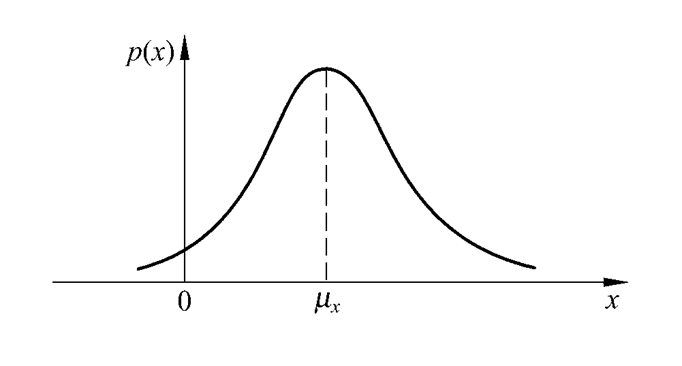
\includegraphics[width=4cm]{Gaussian}
		\caption{高斯(正态)分布随机变量的PDF曲线$\mu_x>0$}
	\end{figure}
    \tiny PDF---概率密度函数(Probability Density Function)
\end{columns}
\end{frame}

\begin{frame}{标准高斯(正态)分布随机变量}
归一化处理$x(\xi)\sim\mathcal{N}(\mu_x,\sigma_x^2)$为$x(\xi)\sim\mathcal{N}(0,1)$, 令
\[u(\xi)=\frac{x(\xi)-\mu_x}{\sigma_x}\]
有
\[p(x)=\left(\frac{1}{2\pi}\right)^{1/2}\exp\left(-\frac{u^2}{2}\right) \]
\begin{columns}
\column{0.4\textwidth}%<1->
\begin{figure}[!h]
	\centering
	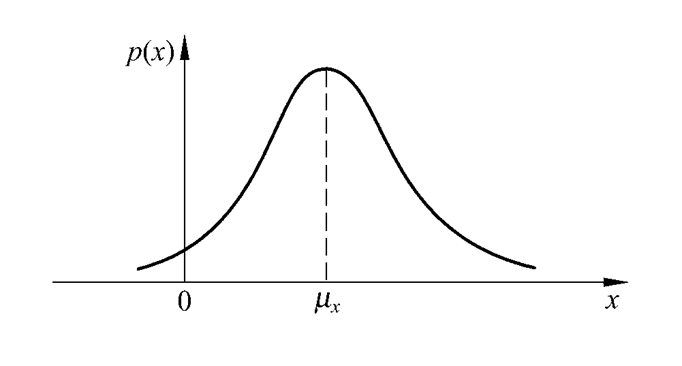
\includegraphics[width=4cm]{Gaussian}
	\caption{高斯(正态)分布随机变量的PDF曲线$\mu_x>0$}
\end{figure}
\column{0.4\textwidth}
\begin{figure}[!h]
	\centering
	\includegraphics[width=4cm]{GaussianN}
	\caption{标准高斯(正态)分布随机变量的PDF曲线$\mu_x=0$}
\end{figure}
\end{columns}
\end{frame}

\begin{frame}{标准高斯(正态)分布随机变量}
\begin{columns}
\column{0.6\textwidth}%<1->
标准高斯分布随机变量的一维累积分布函数(正态概率积分)定义为
\[\Phi(x)\mathop{=}^{def}\int_{-\infty}^{x}\left(\frac{1}{2\pi}\right)^{1/2}\exp\left(-\frac{u^2}{2}\right)du \]
它的互补累积分布函数是标准高斯分布的右尾积分,即
\[Q(x)=1-\Phi(x)\mathop{=}^{def}\int_{x}^{\infty}\left(\frac{1}{2\pi}\right)^{1/2}\exp\left(-\frac{u^2}{2}\right)du \]
\column{0.4\textwidth}
\begin{figure}[!h]
\centering
\includegraphics[width=4cm]{Qx}\\
\caption{标准高斯(正态)分布的右尾积分$Q(x)$}
\end{figure}
\end{columns}
\end{frame}

\begin{frame}{高斯噪声的统计描述(1)}
\begin{definition}[高斯噪声]
	噪声$n(t)$, 对任意$N\ge 1$和所有时刻$t_k$, 随机变量$n(t_k)$服从高斯分布,则$n(t)$为一个高斯噪声随机变量过程,简称高斯噪声过程或高斯噪声。
\end{definition}
\begin{block}{高斯噪声一维概率密度函数}
	\[p(n_k;t_k)=(\frac{1}{2\pi\sigma_{n_k}^2})^{1/2}\exp\left[-\frac{(n_k-\mu_{n_k})^2}{2\sigma_{n_k}^2}\right] \]
	其中,$\mu_{n_k}$为$n(t_k)$的均值, $\sigma_{n_k}$为$n(t_k)$的方差。
\end{block}
\end{frame}

\begin{frame}{高斯噪声的统计描述(2)}
\begin{block}{高斯噪声N维联合概率密度函数}
高斯噪声的N维矢量记为
\[(\bm{n;t})=(n(t_1),n(t_2),\cdots,n(t_N))^T \]
其N维联合概率密度函数为
\begin{align*}
p(\bm{n;t})&=p(n_1,n_2,\cdots,n_N; t_1,t_2,\cdots,t_N)\\
&=\frac{1}{(2\pi)^{N/2}|\bm{C_n}|^{1/2}}\exp\left[-\frac{1}{2}(\bm{n-\mu_n})^T\bm{C_n}^{-1}(\bm{n-\mu_n})\right]
\end{align*}

其中,$\bm{\mu_{n}}$是高斯随机矢量$(\bm{n;t})$的均值矢量,$\bm{C_n}$为协方差矩阵。
即
$$\bm{\mu_n}=(\mu_{n_1},\mu_{n_2},\dots,\mu_{n_N})^T$$
$$\mu_{n_k}=E[n(t_k)]$$
\end{block}
\end{frame}

\begin{frame}
$\bm{C_n}$是高斯随机矢量$\bm{(n;t)}$的协方差
$$
\bm{C_n}=\left[
\begin{matrix}
C_{n_1n_1} & C_{n_1n_2} & \cdots &C_{n_1n_N} \\
C_{n_2n_1} & C_{n_2n_2} & \cdots &C_{n_2n_N} \\
\vdots     &  \vdots    &        &\vdots \\
C_{n_Nn_1} & C_{n_Nn_2} & \cdots &C_{n_Nn_N} \\
\end{matrix}
\right]
$$
其中$C_{n_jn_k}=E[(n(t_j)-\mu_{n_j})(n(t_k)-\mu_{n_k})]=c_{n_k}c_(n_j)$\\
$|\bm{C_n}|$是$\bm{C_n}$的行列式,$\bm{C_n^{-1}}$是$\bm{C_n}$的逆矩阵。
\end{frame}

\begin{frame}{高斯变量$n(t_k)$互不相关$\Leftrightarrow$相互统计独立}
	\begin{block}{不相关性与统计独立性}
		互不相关$\nRightarrow$相互统计独立。但是若$x(t)$服从联合高斯分布,则互不相关$\Leftrightarrow$相互统计独立
	\end{block}
\textbf{证明:} 设高斯随机矢量$\bm{(n;t)}$中的$n(t_j)$与$n(t_k)(j\ne k)$互不相关,即$C_{n_jn_k}=C_{n_kn_j}=0(j\ne k)$, 若记$\sigma_{n_k}^2\mathop{=}\limits^{def}C_{n_kn_k}$,则协方差矩阵$C_n$和$\bm{C_n^{-1}}$分别为
	\begin{columns}
		\column{0.5\textwidth}
		$$
		\bm{C_n}=\left[
		\begin{matrix}
		\sigma_{n_1}^2 &  0                 & \cdots & 0\\
		0              &  \sigma_{n_2}^2  & \cdots & 0\\
		\vdots         &  \vdots            &        &\vdots \\
		0              &  0                 & \cdots &\sigma_{n_N}^2\\
		\end{matrix}
		\right]
		$$
		\column{0.5\textwidth}
		$$\bm{C_n^{-1}}=\left[
		\begin{matrix}
		(\sigma_{n_1}^2)^{-1} &  0                 & \cdots & 0\\
		0              &  (\sigma_{n_2}^2)^{-1}  & \cdots & 0\\
		\vdots         &  \vdots            &        &\vdots \\
		0              &  0                 & \cdots &(\sigma_{n_N}^2)^{-1}\\
		\end{matrix}
		\right]
		$$
	\end{columns}
	而$|\bm{C_n}|^{1/2}$为: $|\bm{C_n}|^{1/2}=\prod\limits_{k=1}^{N}\sigma_{n_k}$
\end{frame}

\begin{frame}
	因此,高斯噪声$n(t)$的N维联合概率密度函数为
	\begin{align*}
	p(\bm{n;t})&=p(n_1,n_2,\cdots,n_N; t_1,t_2,\cdots,t_N)\\
	&=\frac{1}{(2\pi)^{N/2}|\bm{C_n}|^{1/2}}\exp\left[-\frac{1}{2}(\bm{n-\mu_n})^T\bm{C_n}^{-1}(\bm{n-\mu_n})\right]\\
	&=\frac{1}{(2\pi)^{N/2}|\prod\limits_{k=1}^{N}\sigma_{n_k}}\exp\left[-\sum\limits_{k=1}^{N}\frac{(n_k-\mu_{n_k})^2}{2\sigma_{n_k}^2}\right]\\
	&=\prod\limits_{k=1}^{N}\left(\frac{1}{2\pi\sigma_{n_k}}\right)^{1/2}\exp\left[-\frac{(n_k-\mu_{n_k})^2}{2\sigma_{n_k}^2}\right]\\
	&=p(x_1;t_1)p(x_2;t_2)\cdots p(x_N;t_N)
	\end{align*}
	表明$n(t)$的N维联合概率密度函数表示成各自一维概率密度函数之积的形式,即是统计独立性的定义。因此,\textbf{N个高斯随机变量$n(t_k)(k=1,2,\dots,t_N)$互不相关$\Rightarrow$相互统计独立}; 结合之前的结论``相互统计独立的随机变量$\Rightarrow$互不相关''。所以, \textbf{
	N个高斯随机变量$n(t_k)(k=1,2,\dots,t_N)$互不相关$\Leftrightarrow$相互统计独立}。
\end{frame}

\begin{frame}{高斯随机变量的线性组合仍然是高斯随机变量}
\begin{enumerate}
	\item 若$x_k(\xi)\sim\mathcal{N}(\mu_{x_k},\sigma_{x_k}^2)(k=1,2,\dots,N)$,且它们相互统计独立,则它们的和
	\[x(\xi)=\sum\limits_{k=1}^{N}x_k(\xi) \]
	是高斯随机变量,且有$x_k(\xi)\sim\mathcal{N}(\mu_x,\sigma_x^2)$,其中
	$\mu_x=\sum\limits_{k=1}^N\mu_{x_k},\sigma_x^2=\sum\limits_{k=1}^N\sigma_{x_k}^2$
	\item 更一般地,任意有限N个高斯随机变量$x_k(\xi)(k=1,2,\dots,N)$的线性组合
	\[x(\xi)=\sum\limits_{k=1}^{N}a_kx_k(\xi) \]
	仍然是高斯随机变量,且有$x_k(\xi)\sim\mathcal{N}(\mu_x,\sigma_x^2)$,其中
	$\mu_x=\sum\limits_{k=1}^Na_k\mu_{x_k},\sigma_x^2=\sum\limits_{j=1}^N\sum\limits_{k=1}^Na_ja_kc_{x_kx_j}$\\
	式中,协方差函数$c_{x_jx_k}=E[(x_j(\xi)-\mu_{x_j})(x_k(\xi)-\mu_{x_k})]=c_{x_kx_j},\mu_{x_k}=E[x_k(\xi)]$
\end{enumerate}
\end{frame}

\begin{frame}
\begin{example}
	设随机变量$y$与$x$之间为线性关系$y=ax+b,a,b$为常数,且$a\ne 0$。已知随机变量$x$服从高斯分布,即
	\[p(x)=\left(\frac{1}{2\pi\sigma_x^2}\right)^{1/2}\exp\left[-\frac{(x-\mu_x)^2}{2\sigma_x^2}\right] \]
	证明随机变量$y$是服从均值为$a\mu_x+b$, 方差为$a^2\sigma_x^2$的高斯分布。
\end{example}
\end{frame}

\begin{frame}
\begin{proof}
证法I: 雅可比变换法
\begin{align*}
&\text{因为}\qquad  y=ax+b \\
&\text{所以,反函数为}\qquad  x=\frac{y-b}{a} \\
&\text{且有}\qquad  \frac{dx}{dy}=\frac{1}{a} \\
&\text{于是,由一维雅可比变换,得}  \\
&p(y)=\left(\frac{1}{2\pi\sigma_x^2}\right)^{1/2}\exp\left[-\frac{(\frac{y-b}{a}-\mu_x)^2}{2\sigma_x^2}\right]\left|\frac{1}{a}\right| \\
&=\left(\frac{1}{2\pi  a^2\sigma_x^2}\right)^{1/2}\exp\left[-\frac{(y-(a\mu_x+b))^2}{2a^2\sigma_x^2}\right]  
\end{align*}
所以,随机变量$y$是服从均值为$a\mu_x+b$, 方差为$a^2\sigma_x^2$的高斯分布。
\end{proof}
\end{frame}

\begin{frame}
\begin{proof}
证法II: 利用高斯随机变量的特性来证明\\
因为  $y=ax+b$ \\
是高斯随机变量$x$的线性变换,所以$y$仍然是高斯随机变量。\\
其均值$\mu_y$和方差$\sigma_y^2$分别为
\begin{align*}
\mu_y&=E(y)=E(ax+b)=aE(x)+b\\
&=a\mu_x+b\\
\sigma_y^2&=E[(y-\mu_y)^2]=E[(ax+b-a\mu_x-b)^2]\\
&=a^2E[(x-\mu_x)^2]\\
&=a^2\sigma_x^2
\end{align*}
所以,随机变量$y$是服从均值为$a\mu_x+b$, 方差为$a^2\sigma_x^2$的高斯分布。
\end{proof}
\end{frame}

\begin{frame}{白噪声}
\small
%白噪声的频域,时域描述:
\begin{columns}%0.6 0.4表示相对比例
	\column{0.6\textwidth}
	\begin{block}{频域---白噪声的功率谱密度}
	功率谱密度均匀分布在整个频率轴上: $p_n(\omega)=\frac{N_0}{2},\quad -\infty<\omega< \infty, N_0$是常数\\
	也可以按正半轴上的频域定义: $p_n(\omega)=N_0,\quad 0<\omega<\infty, N_0$是常数
	\end{block}
    \column{0.3\textwidth}
    \includegraphics[scale=0.3]{WhiteNoise2}
\end{columns}

\begin{columns}%0.6 0.4表示相对比例
	\column{0.6\textwidth}
	\begin{block}{时域---白噪声的自相关函数}
	均值为零、自相关函数$r_n(\tau)$为$\delta$的噪声随机过程: $r_n(\tau)=IFT[\frac{N_0}{2}]=\frac{N_0}{2}\delta(\tau)$
	\end{block}
	\column{0.3\textwidth}
	\includegraphics[scale=0.3]{WhiteNoise1}
\end{columns}
\begin{block}{意义}
	白噪声是一种理想化的数学模型,由于其功率谱密度在整个频域上均匀分布,所以其能量是无限的,实际上是不存在的。但是由于我们所采用的系统相对于整个频率轴来说是窄带系统,只要认为频谱是均匀分布的,能够在数学上带来很大方便。
\end{block}
\end{frame}

\begin{frame}{白噪声特性}
\includegraphics[scale=0.4]{WhiteNoise}
\begin{block}{白噪声$n(t)$重要特性}
	\begin{itemize}
		\item 白噪声在频域上其功率谱密度是均匀分布的;
		\item 时域上自相关函数$r_n(\tau)$是$\delta$函数: $r_n(\tau)=IFT[\frac{N_0}{2}]=\frac{N_0}{2}\delta(\tau)$
		\item 任意两个不同时刻的随机变量$n(t_j)$与$n(t_k),(\tau=t_j-t_k\ne 0)$是不相关的:\\
		$r_n(t_j,t_k)=r_n(\tau)=E[n(t_j)n(t_k)]=0,(\tau=t_j-t_k\ne 0)$。
		\item 由于$\delta$---函数的筛选性: $\int_{-\infty}^{\infty}\delta(t-t_0)f(t)dt=f(t_0)$,有\\
		$\int_{-\infty}^{\infty}r_n(t-t_0)f(t)dt=f(t_0)=\frac{N_0}{2}\int_{-\infty}^{\infty}\delta(t-t_0)f(t)dt=\frac{N_0}{2}f(t_0)$
	\end{itemize}	
\end{block}
\end{frame}

\begin{frame}{高斯白噪声}
\begin{block}{高斯白噪声$n(t)$重要特性---高斯随机变量+白噪声}
	\begin{itemize}
		\item 高斯白噪声在频域上其功率谱密度是均匀分布的;
		\item \textbf{时域上概率密度函数是高斯分布的。(白噪声对此没有明确限制)}
		\item 时域上自相关函数$r_n(\tau)$是$\delta$函数: $r_n(\tau)=IFT[\frac{N_0}{2}]=\frac{N_0}{2}\delta(\tau)$
		\item 任意两个不同时刻的随机变量$n(t_j)$与$n(t_k),(\tau=t_j-t_k\ne 0)$是不相关的,\textbf{并且是统计独立的}:\\
		$r_n(t_j,t_k)=r_n(\tau)=E[n(t_j)n(t_k)]=0,(\tau=t_j-t_k\ne 0)$。
		\item 由$\delta$---函数的筛选性: $\int_{-\infty}^{\infty}\delta(t-t_0)f(t)dt=f(t_0)$,有\\
		$\int_{-\infty}^{\infty}r_n(t-t_0)f(t)dt=f(t_0)=\frac{N_0}{2}\int_{-\infty}^{\infty}\delta(t-t_0)f(t)dt=\frac{N_0}{2}f(t_0)$
	\end{itemize}	
\end{block}
\includegraphics[scale=0.4]{WhiteGaussianNoise}
\end{frame}

\begin{frame}{有色噪声}
如果噪声过程$n(t)$的功率谱密度在频域上的分布是不均匀的,则称其为有色噪声。
\begin{block}{有色噪声的功率谱密度}
	\[P_n(f) =P_0\exp\left[-\frac{(f-f_0)^2}{2\sigma_f^2}\right]\]
	均值$f_0$代表频谱的中心频率,方差$\sigma_f^2$反映噪声的谱宽度。$\omega=2\pi f$
\end{block}
\end{frame}

\begin{frame}[shrink]
\frametitle{ch2.信号检测与估计理论的基础知识}
\tableofcontents[hideallsubsections]
\end{frame}


 % ch2 随机过程
%%%%%%%%%%%%%%%%%%%%%%%%%%% ch2-StochasticProcess
\begin{frame}[shrink]
\frametitle{ch2. Example}
\tableofcontents%[hideallsubsections]
\end{frame}

\section{习题}

\begin{frame}{均匀分布随机变量$x$的均值$\mu_x$和方差$\sigma_x^2$}
\begin{example}
求如图均匀分布随机变量$x$的均值$\mu_x$和方差$\sigma_x^2$。
\includegraphics[scale=0.3]{ex2-1}
\end{example}
\end{frame}

\begin{frame}{均匀分布随机变量$x$的均值$\mu_x$和方差$\sigma_x^2$}
解: 随机变量$x$的概率密度函数$p(x)$为
\[p(x)=\begin{cases}
\frac{1}{b-1}, &a\le x\le b\\
0, &\text{其他}
\end{cases} \]

	根据随机变量均值的定义,有
	\begin{align*}
	\mu_x=E(x)&=\int_{-\infty}^{\infty}xp(x)dx=\int_{a}^{b}\frac{1}{b-1}p(x)dx =\frac{a+b}{2}
	\end{align*}
	根据随机变量方差的定义,有
	\begin{align*}
	\sigma_x^2=E[(x-\mu_x)^2]&=\int_{-\infty}^{\infty}(x-\mu_x)^2p(x)dx=\int_{a}^{b}\left(x-\frac{a+b}{2}\right)^2\frac{1}{b-a}dx \\
	&=\frac{(b-a)^2}{12}
	\end{align*}	
\end{frame}

\begin{frame}{高斯变量的线性组合仍然是高斯随机变量}
\begin{example}
	设随机变量$y$与$x$之间为线性关系$y=ax+b,a,b$为常数,且$a\ne 0$。已知随机变量$x$服从高斯分布,即
	\[p(x)=\left(\frac{1}{2\pi\sigma_x^2}\right)^{1/2}\exp\left[-\frac{(x-\mu_x)^2}{2\sigma_x^2}\right] \]
	证明随机变量$y$是服从均值为$a\mu_x+b$, 方差为$a^2\sigma_x^2$的高斯分布。
\end{example}
\end{frame}

\begin{frame}
\begin{proof}
	证法I: 雅可比变换法
	\begin{align*}
		&\text{因为}\qquad  y=ax+b \\
		&\text{所以,反函数为}\qquad  x=\frac{y-b}{a} \\
		&\text{且有}\qquad  \frac{dx}{dy}=\frac{1}{a} \\
		&\text{于是,由一维雅可比变换,得}  \\
		&p(y)=\left(\frac{1}{2\pi\sigma_x^2}\right)^{1/2}\exp\left[-\frac{(\frac{y-b}{a}-\mu_x)^2}{2\sigma_x^2}\right]\left|\frac{1}{a}\right| \\
		&=\left(\frac{1}{2\pi  a^2\sigma_x^2}\right)^{1/2}\exp\left[-\frac{(y-(a\mu_x+b))^2}{2a^2\sigma_x^2}\right]  
	\end{align*}
	所以,随机变量$y$是服从均值为$a\mu_x+b$, 方差为$a^2\sigma_x^2$的高斯分布。
\end{proof}
\end{frame}

\begin{frame}
\begin{proof}
	证法II: 利用高斯随机变量的特性来证明\\
	因为  $y=ax+b$ \\
	是高斯随机变量$x$的线性变换,所以$y$仍然是高斯随机变量。\\
	其均值$\mu_y$和方差$\sigma_y^2$分别为
	\begin{align*}
	\mu_y&=E(y)=E(ax+b)=aE(x)+b\\
	&=a\mu_x+b\\
	\sigma_y^2&=E[(y-\mu_y)^2]=E[(ax+b-a\mu_x-b)^2]\\
	&=a^2E[(x-\mu_x)^2]\\
	&=a^2\sigma_x^2
	\end{align*}
	所以,随机变量$y$是服从均值为$a\mu_x+b$, 方差为$a^2\sigma_x^2$的高斯分布。
\end{proof}
\end{frame}

\begin{frame}{周期性锯齿波}
\begin{example}
设随机过程的样本函数是周期性的锯齿波,下图是它的两个样本函数。各样本函数具有相同的波形,其区别在于锯齿波的起点位置不同。设在$t=0$后的第一个值位于$\tau,\tau$是一个随机变量,它在$(0,T)$上服从均匀分布。若锯齿波的幅度为常数$A$, 求该随机过程$x(t)$的一维概率密度函数。
\includegraphics[scale=0.2]{ex2-11}
\end{example}
\end{frame}

\begin{frame}
解: 因为是周期性锯齿波, 所以只需求出一个周期的概率密度函数。
在一个周期内,随机信号为
\[x(t)=\frac{A}{T}(t+T-\tau),\quad t-T\le t\le\tau \]
其反函数$\tau$为
\[\tau=T-\frac{T}{A}x(t)+t,\quad 0\le\tau\le T,0\le x\le A \]
因为随机变量$\tau$在$(0,T)$上脉冲均匀分布,即
\[
p(\tau)=\begin{cases}
\frac{1}{T},&0\le\tau\le T\\
0,&\text{其它}
\end{cases} 
\]
所以,由一维雅可比变换,得
\begin{align*}
p(x;t)&=p[\tau=h(x)]\left|\frac{d\tau}{dx}\right|\\
&=\begin{cases}
\frac{1}{T}\frac{T}{A}\\
0
\end{cases}
=\begin{cases}
\frac{1}{A}, &0\le x\le A\\
0,&\text{其它}
\end{cases}
\end{align*}
\end{frame}

\begin{frame}{确知函数$a(t)$的均值$E[a(t)]=a(t)$}
\begin{example}
设随机过程$x(t)$的均值为$\mu_x(t)$,自相关函数为$r_x(t_j,t_k)$。若有随机过程$y(t)=a(t)x(t)x(t)+b(t)$, 其中$a(t),b(t)$是确知函数。求随机过程$y(t)$的均值和自相关函数。
\end{example}
\end{frame}

\begin{frame}{确知函数$a(t)$的均值$E[a(t)]=a(t)$}
解:\\
由均值定义$E[x(\xi)]\mathop{=}\limits^{def}\mu_x=\int_{-\infty}^{\infty}xp(x)dx$知:\\
确知函数$a(t)$的均值:
\begin{align*}
E[a(t)]&=\int_{-\infty}^{\infty}a(t)p(x)dx\\
&=a(t)\int_{-\infty}^{\infty}p(x)dx &&\text{by $a(t)$是常数}\\
&=a(t)\cdot 1 &&by \int_{-\infty}^{\infty}p(x)dx=1\\
&=a(t)
\end{align*}
\end{frame}

\begin{frame}{确知函数$a(t)$的均值$E[a(t)]=a(t)$}
解(续):随机过程$y(t)$的均值为:
\begin{align*}
\mu_y&=E[y(t)]=E[a(t)x(t)+b(t)]=E[a(t)x(t)]+E[b(t)]\\
&=a(t)E[x(t)]+b(t)=a(t)\mu_x+b(t)
\end{align*}
随机过程$y(t)$的自相关函数为:
\begin{align*}
\r_y(t_j,t_k)&=E[y(t_j)y(t_k)]\\
&=E[(a(t_j)x(t_j)]+b(t_j))(a(t_k)x(t_k)+b(t_k))]\\
&=a(t_j)a(t_k)E[x(t_j)]x(t_k)]+a(t_j)b(t_k)E[x(t_j)]+b(t_j)a(t_k)E[x(t_k)]+b(t_j)b(t_k)\\
&=a(t_j)a(t_k)r_x(t_j,t_k)+a(t_j)b(t_k)\mu_x(t_j)+b(t_j)a(t_k)\mu_x(t_k)+b(t_j)b(t_k)
\end{align*}
其中: $\mu_x(t_k)=E[x(t_k)],r_x(t_j,t_k)=E[x(t_j)x(t_k)]$
\end{frame}

\begin{frame}{平稳随机过程随着间隔的增大,采样之间的相关性减小}
\begin{example}
	对于平稳随机过程$x(t)$, 随着间隔$\tau$的增大,随机过程采样之间的相关性减小,即满足
	\[\lim\limits_{\tau\to\infty}c_x(\tau)=0 \]
	证明: (1) $r_x(\infty)=\mu_x^2$;\qquad  (2) $r_x(0)-r_x(\infty)=\sigma_x^2$
\end{example}
\end{frame}

\begin{frame}[shrink]
\begin{proof}
	(1) 因为 
		$$r_x(\tau)=c_x(\tau)+\mu_x^2$$
		所以
		$$\lim\limits_{\tau\to\infty}r_x(\tau)=\lim\limits_{\tau\to\infty}c_x(\tau)+\mu_x^2$$
		当
		$$\lim\limits_{\tau\to\infty}c_x(\tau)=0$$
		时,有
		$$\lim\limits_{\tau\to\infty}r_x(\tau)=r_x(\infty)=\mu_x^2$$
	(2) 因为
		$$r_x(0)=E[x(t)x(t)]=E[x^2(t)] $$
		而
		$$r_x(\infty)=\mu_x^2$$
		于是
		$$r_x(0)-r_x(\infty)=E[x^2(t)]-\mu_x^2=\sigma_x^2$$
\end{proof}
\end{frame}

\begin{frame}{周期性平稳过程的自相关函数也是周期性,且周期相同}
\begin{example}
	假定平稳随机过程$x(t)$是周期的, 周期为$T$, 即
	\[x(t)=x(t+T) \]
	证明其自相关函数$r_x(\tau)$也是以$T$为周期的, 即
	\[r_x(\tau)=r_x(\tau+T) \]
\end{example}
\end{frame}

\begin{frame}{周期性平稳过程的自相关函数也是周期性,且周期相同}
\begin{example}
	假定平稳随机过程$x(t)$是周期的, 周期为$T$, 即
	\[x(t)=x(t+T) \]
	证明其自相关函数$r_x(\tau)$也是以$T$为周期的, 即
	\[r_x(\tau)=r_x(\tau+T) \]
\end{example}
\begin{proof}
因为
\begin{align*}
r_x(\tau)&=E[x(t)x(t+\tau)]\\
&=E[x(t)x(t+\tau+T)]&& \text{by } x(t+\tau)=x(t+\tau+T)\\
&=r_x(\tau+T)
\end{align*}
\end{proof}
\end{frame}

\begin{frame}{联合平稳的随机过程}
\begin{example}
	设$x(t)$和$y(t)$是联合平稳的随机过程, 试证明:
	\begin{enumerate}
		\item $r_{xy}(\tau)=r_{yx}(-\tau),c_{xy}(\tau)=c_{yx}(-\tau)$
		\item $|r_{xy}(\tau)|^2\le r_x(0)r_y(0)$
		\item $|\rho_{xy}(\tau)\le 1$
	\end{enumerate}
\end{example}
\end{frame}

\begin{frame}{联合平稳的随机过程}
\begin{proof}
	\begin{enumerate}
		\item \begin{align*}
		r_{xy}(\tau)&=E[x(t)y(t+\tau)]=E[y(t+\tau)x(t)]=r_{xy}(-\tau)\\
		c_xy(\tau)&=E[(x(t)-\mu_x(t))(y(t+\tau)-\mu_y(t+\tau))]\\
		&=E[(y(t+\tau)-\mu_y(t+\tau))(x(t)-\mu_x(t))]\\
		&=c_{yx}(-\tau)
		\end{align*}
		\item \begin{align*}
		|r_{xy}(\tau)|^2&=|E[x(t)y(t+\tau)]|^2\le (E|x(t)y(t+\tau)|)^2\\
		&\le E|x(t)|^2E|y(t+\tau)|^2=r_x(0)r_y(0)
		\end{align*}
	\end{enumerate}
\end{proof}
\end{frame}

\begin{frame}{联合平稳的随机过程}
\begin{proof}
	\begin{enumerate}
		\setcounter{enumi}{2} %设定起始编号 
		\item 因为 
		\begin{align*}
		|c_{xy}(\tau)|^2&=|E[(x(t)-\mu_x(t))(y(t+\tau)-\mu_y(t+\tau))]|^2\\
		&\le E|(x(t)-\mu_x(t))|^2E|(y(t+\tau)-\mu_y(t+\tau))|^2\\
		&=c_x(0)c_y(0)=\sigma_x^2\sigma_y^2
		\end{align*}
		所以 
		\[|c_{xy}(\tau)|\le\sigma_x\sigma_y \]
		从而得
		\[|\rho_{xy}(\tau)|=\frac{|c_{xy}(\tau)|}{\sigma_x\sigma_y}\le 1 \]
	\end{enumerate}
\end{proof}
\end{frame}

\begin{frame}{雷达回波信号}
\begin{example}
	设$s(t)$是雷达的发射信号, 遇到目标后的反射信号为$as(t-t_0), t_0$是信号返回的延迟时间。如果回波信号中伴有加性噪声$n(t)$, 则接收到的信号为
	\[x(t)=as(t-t_0)+n(t) \]
	\begin{enumerate}
		\item 假定$s(t)$和$n(t)$是平稳相关的, 试求互相关函数$r_sx(\tau)$。
		\item 如果噪声$n(t)$的均值为零, 且与$s(t)$相互统计独立, 试求互相关函数$r_sx(\tau)$。
	\end{enumerate}
\end{example}
\end{frame}

\begin{frame}[shrink]
解:
	\begin{enumerate}
		\item 假定$s(t)$和$n(t)$是平稳相关的, 试求互相关函数$r_sx(\tau)$。\begin{align*}
		r_{xy}(\tau)&=E[s(t)x(t+\tau)] \\
		&=E[s(t)(as(t-t_0+\tau)+n(t+\tau)))] &&\text{by } x(t)=as(t-t_0)+n(t)\\
		&=aE[s(t)s(t-t_0+\tau)]+E[s(t)n(t+\tau)]\\
		&=ar_{s}(\tau-t_0)+r_{sn}(\tau)
		\end{align*}
		\item 如果噪声$n(t)$的均值为零, 且与$s(t)$相互统计独立, 试求互相关函数$r_sx(\tau)$。
		\begin{align*}
		r_{xy}(\tau)&=E[s(t)x(t+\tau)] \\
		&=E[s(t)(as(t-t_0+\tau)+n(t+\tau)))] &&\text{by } x(t)=as(t-t_0)+n(t)\\
		&=aE[s(t)s(t-t_0+\tau)]+E[s(t)n(t+\tau)] &&\text{确知信号$s(t)$看作常数}\\ 
		&=aE[s(t)s(t-t_0+\tau)]+s(t)E[n(t+\tau)] &&\text{by }E[n(t)]=0 \\
		&=ar_{s}(\tau-t_0)+r_{sn}(\tau)
		\end{align*}
	\end{enumerate}
\end{frame}

 % ch2习题,已整合至ch-part1和ch2-StochasticProcess中
%%%%%%%%%%%%%%%%%%%% ch1,ch2共5次课,第5次课后45分钟作业: 雷达回波信号, y=ax+b
%%%%%%%%%%%%%%%%%%%%%%%%%%%%%%% ch3
%%%%%%%%%%%%%%%%%%%%%%%%%%% ch3
\begin{frame}
  \frametitle{主要内容}
  \tableofcontents[hideallsubsections]
\end{frame}

\section{准备知识}
\begin{frame}
\begin{theorem}
	如果函数$f(x)$在区间$[a,b]$上连续,则积分上限函数
	\[\Phi(x)=\int_a^x f(t)dt\]
	在[a,b]上具有导数,并且它的导数是
	\[\Phi^\prime(x)=\frac{d}{dx}\int_a^xf(t)dt=f(x)\qquad (a\le x\le b) \]
\end{theorem}
\begin{theorem}
	如果函数$f(x)$在区间$[a,b]$上连续,则函数
	\[\Phi(x)=\int_a^x f(t)dt\]	
	就是$f(x)$在$[a,b]$上的一个原函数。
\end{theorem}
\end{frame}

\begin{frame}
\begin{theorem}
	如果函数$F(x)$是连续函数$f(x)$在区间$[a,b]$上的一个原函数,则
	\[\int_a^b f(x)dx=F(b)-F(a)\]	
\end{theorem}
\end{frame}

\begin{frame}
似然比检验的判别式:
\[\lambda(x)=\frac{p(x|H_1)}{p(x|H_0)}\mathop{\gtrless}_{H_0}^{H_1}\eta \]
判决概率:
\[P_F=P(H_1|H_0)=\int_{\eta}^{\infty}p(\lambda|H_0)d\lambda \]
\[P_D=P(H_1|H_1)=\int_{\eta}^{\infty}p(\lambda|H_1)d\lambda \]
\end{frame}

\begin{frame}
\begin{align*}
&P_D =P_D=P(H_1|H_1)=\int_{\eta}^{\infty}p(\lambda|H_1)d\lambda=P_D(\eta) \\
&P_F =P(H_1|H_0)=\int_{\eta}^{\infty}p(\lambda|H_0)d\lambda=P_F(\eta) \\
&\frac{dP_D(\eta)}{d\eta} =-p(\eta|H_1) \\ 
&\frac{dP_F(\eta)}{d\eta} =-p(\eta|H_0) \\ 
&\qquad \text{ by } \Phi^\prime(x)=\frac{d}{dx}\int_a^xf(t)dt=f(x)\qquad (a\le x\le b) \\
&\frac{dP_D(\eta)}{dP_F(\eta)} =\frac{-p(\eta|H_1)}{-p(\eta|H_0)}=\frac{p(\eta|H_1)}{p(\eta|H_0)}\\
\end{align*}
\end{frame}

\begin{frame}
\begin{align*}
P_D(\eta) &=P[(\lambda|H_1)\ge\eta]&\\
&=\int_{\eta}^{\infty}p(\lambda|H_1)d\lambda&\\
&=\int_{R_1}^{\infty}p(x|H_1)dx&\\
&=\int_{R_1}^{\infty}\lambda p(x|H_0)dx &\text{ by }\lambda(x)=\frac{p(x|H_1)}{p(x|H_0)}\mathop{\gtrless}_{H_0}^{H_1}\eta&\\
&=\int_{\eta}^{\infty}\lambda p(\lambda|H_0)d\lambda&
\end{align*}
\[\frac{dP_D(\eta)}{d\eta}=-\eta p(\eta|H_0)\]
\[\frac{dP_D(\eta)}{dP_F(\eta)}=\frac{-p(\eta|H_1)}{-p(\eta|H_0)}=\frac{-\eta p(\eta|H_0)}{-p(\eta|H_0)}=\eta \]  
\end{frame}

\begin{frame}
$H_1$含随机变量$m$的似然比检验的判别式:
\[\lambda(x)=\frac{p(x|m; H_1)}{p(x|H_0)}=\frac{\int_{-\infty}^{\infty}p(x|m,H_1)p(m)dm}{p(x|H_0)}\mathop{\gtrless}_{H_0}^{H_1}\eta \]
\end{frame}

\begin{frame}
$p(m)$未知
\begin{align*}
&p(x|H_0)=(\frac{1}{2\pi\sigma_n^2})^{1/2}\exp(-\frac{x^2}{2\sigma_n^2})\\
&p(x|m;H_1)=(\frac{1}{2\pi\sigma_n^2})^{1/2}\exp(-\frac{(x-m)^2}{2\sigma_n^2})\\
&\lambda(x)=\frac{p(x|m; H_1)}{p(x|H_0)}\mathop{\gtrless}_{H_0}^{H_1}\eta\\
&\exp(\frac{2mx}{2\sigma_n^2}-\frac{m^2}{2\sigma_n^2})\mathop{\gtrless}_{H_0}^{H_1}\eta\\
&mx\mathop{\gtrless}_{H_0}^{H_1}\sigma_n^2\ln\eta+\frac{m^2}{2}
\end{align*}
\end{frame}

\begin{frame}
\begin{align*}
&m_0\le m\le m_1,m_0>0\\
&mx\mathop{\gtrless}_{H_0}^{H_1}\sigma_n^2\ln\eta+\frac{m^2}{2}\\
&l(x)=x\mathop{\gtrless}_{H_0}^{H_1}\frac{\sigma_n^2}{m}\ln\eta+\frac{m}{2}\mathop{=}^{def}\gamma^+\\
&\int_{\gamma^+}^{\infty}(\frac{1}{2\pi\sigma_n^2})^{1/2}\exp(-\frac{l^2}{2\sigma_n^2})dl=\alpha
\end{align*}
\end{frame}

\begin{frame}
\begin{align*}
&m_0\le m\le m_1,m_1<00\\
&mx\mathop{\gtrless}_{H_0}^{H_1}\sigma_n^2\ln\eta+\frac{m^2}{2}\\
&l(x)=x\mathop{\lessgtr}_{H_0}^{H_1}-\frac{\sigma_n^2}{|m|}\ln\eta-\frac{|m|}{2}\mathop{=}^{def}\gamma^-\\
&\int_{-\infty}^{\gamma^-}(\frac{1}{2\pi\sigma_n^2})^{1/2}\exp(-\frac{l^2}{2\sigma_n^2})dl=\alpha
\end{align*}
\end{frame}

\begin{frame}
若$m_0>0$, $m$仅取正值, 则在$P(H_1|H_0)=\alpha$的约束下, $P^{(m)}(H_1|H_1)$是最大的,其一致最大功效检验成立;\\
若$m_1<0$, $m$仅取负值, 则在$P(H_1|H_0)=\alpha$的约束下, $P^{(m)}(H_1|H_1)$也是最大的。
\end{frame}

\begin{frame}
若$m_0<0,m_1>0$, 即$m$取值可能为正或可能为负的情况下, 无论参量信号的统计检测,按$m$仅取正值设计,还是按$m$仅取负值设计,都有可能在某些$m$值下,   $P^{(m)}(H_1|H_1)$不满足最大的要求。\\
例如,按$m$取正设计信号检测系统,当$m$为正时,$P^{(m)}(H_1|H_1)$最大, 但当$m$为负时, $P^{(m)}(H_1|H_1)$可能最小。\\
因此, 这种情况下不能采用奈曼-皮尔逊准则来实际最佳检测系统。
\end{frame}

\begin{frame}
若$m_0<0,m_1>0$, 即$m$取值可能为正或可能为负,奈曼-皮尔逊准则不能保证$P^{(m)}(H_1|H_1)$最大要求。考虑把约束条件$P(H_1|H_0)=\alpha$分成两个$\alpha/2$, 假设$H_1成立$的判决域由两部分组成。判决表示式为
	\[|x|\mathop{\gtrless}_{H_0}^{H_1}\gamma \]

\begin{block}{}
	虽然双边检验比均值$m$假定为正确时的单边检验性能差,但是比均值$m$假定为错误时的单边检验性能要好的多。因此不失为一种好的折中方法。
\end{block}
\end{frame}

\begin{frame}{广义似然比检验}
\begin{align*}
&\text{似然函数}\\
&p(x|m;H_1)=(\frac{1}{2\pi\sigma_n^2})^{1/2}\exp(-\frac{(x-m)^2}{2\sigma_n^2})\\
&\text{对$m$求偏导,令结果等于零,即} \\
&\frac{\partial\ln p(x|m;H_1)}{\partial m}|_{m=\widehat{m}_{ml}}=0\\
&\text{解得单次观测时,$m$的最大似然估计量$\widehat{m}_{ml}=x$, 于是有 }\\
&p(x|\widehat{m}_{ml};H_1)=(\frac{1}{2\pi\sigma_n^2})^{1/2}\exp(-\frac{(x-\widehat{m}_{ml})^2}{2\sigma_n^2})|_{\widehat{m}_{ml}=x}=(\frac{1}{2\pi\sigma_n^2})^{1/2}\\
\end{align*}
\end{frame}
\begin{frame}{广义似然比检验}
\begin{align*}
&p(x|H_0)=(\frac{1}{2\pi\sigma_n^2})^{1/2}\exp(-\frac{x^2}{2\sigma_n^2})
&p(x|\widehat{m}_{ml};H_1)=(\frac{1}{2\pi\sigma_n^2})^{1/2}\\
&\text{代入广义似然比检验中, 有}\\
&\lambda(x)=\frac{p(x|m; H_1)}{p(x|H_0)}\mathop{\gtrless}_{H_0}^{H_1}\eta\\
&\lambda(x)=\frac{(\frac{1}{2\pi\sigma_n^2})^{1/2}}{(\frac{1}{2\pi\sigma_n^2})^{1/2}\exp(-\frac{x^2}{2\sigma_n^2})}\mathop{\gtrless}_{H_0}^{H_1}\eta\\
&\text{化简得判决表示式}
&x^2\mathop{\gtrless}_{H_0}^{H_1}2\sigma_n^2\ln\eta\mathop{=}^{def}\gamma^2 \implies |x|\mathop{\gtrless}_{H_0}^{H_1}\gamma
\end{align*}
这正是前面讨论过的双边检验。只是前面是从奈曼-皮尔逊准则出发推导得到。而这里是从似然比检验的概念导出的,似然函数$p(x|m;H_1)$中的信号参量$m$由其最大似然估计量$\widehat{m}_{ml}$代换,所以是广义似然比检验。
\end{frame}

  % 部分公式
%%%%%%%%%%%%%%%%%%%%%%%%%%%ch3-1
\begin{frame}[shrink]
  \frametitle{ch3.信号检测与估计理论的基础知识}
  \framesubtitle{ch3-1. 统计检测理论基本概念及贝叶斯准则}
  \tableofcontents[hideallsubsections]
\end{frame}

\section{统计检测理论基本概念}

\begin{frame}{统计检测理论(假设检验理论)}
\begin{itemize}
	\item 统计信号处理的理论基础之一
	\item 主要研究在受噪声干扰的随机信号中,信号的有/无或信号属于哪个状态的最佳判决的概念、方法和性能等问题。
	\item 数学基础——统计判决理论,又称假设检验理论
\end{itemize}
\end{frame}

\begin{frame}{经典的信号统计检测理论}
\begin{itemize}
	\item 统计信号检测理论的基本概念
	\item 二元信号检测的最佳检测准则
	\item 信号状态的判决的方法和检测性能的分析
	\item M元信号的最佳检测
	\item 参量信号的复合假设检验
	\item 序列检测
\end{itemize}
\end{frame}

\section{二元信号检测}

\begin{frame}{统计检测理论的基本模型: 二元信号检测的模型}
\includegraphics[scale=0.3]{model}
\begin{align*}
\textbf{信源}\implies &\text{\textcolor{blue}{信源的输出称为假设}}\\
\textbf{概率转移机构}\implies &\text{\textcolor{blue}{将信源的输出(假设)以一定的}}\\
&\text{\textcolor{blue}{概率关系映射到整个观察空间中}}\\
\textbf{观测空间}\implies &\text{\textcolor{blue}{接收端所有可能观测量的集合}}\\
\textbf{判决规则}\implies &\text{\textcolor{blue}{将观测空间进行合理划分, }}\\
&\text{\textcolor{blue}{使每个观测量对应一个假设判断的方法}}\\
\end{align*}
\end{frame}

\begin{frame}{统计检测理论的基本模型: 二元信号检测的模型示例1}
\begin{columns}
	\column{0.3\textwidth}
	\begin{align*}
	&H_1: r=1+n\\
	&H_0: r=-1+n\\
	&n:\text{噪声是一随机变量}\\
	&\text{一维观测空间:}\\
	&\bm{R}=\{-2,-1,0,1,2\}
	\end{align*}
	\column{0.7\textwidth}
	\includegraphics[scale=0.45]{ex-1m}\\
	\includegraphics[scale=0.45]{ex-1}
\end{columns}
\end{frame}

\begin{frame}{统计检测理论的基本模型: 二元信号检测的模型示例2}
\begin{columns}
	\column{0.3\textwidth}
	\begin{align*}
	H_1: &r_1=1+n_1\\
	&r_2=1+n_2\\
	H_0: &r_1=-1+n_1\\
	&r_2=-1+n_2
	\end{align*}
	\begin{align*}
	&n_1,n_2:\text{噪声}\\
	&\text{二维观测空间:}\\
	&\bm{R}=\{R_1,R_2\}
	\end{align*}
	\column{0.7\textwidth}
	\includegraphics[scale=0.45]{ex-2m}\\
	\includegraphics[scale=0.45]{ex-2}
\end{columns}
\end{frame}

\begin{frame}{统计检测理论的基本模型: 二元信号检测的判决域}
\begin{columns}
	\column{0.5\textwidth}
	二元信号的检测问题,可归结为\textcolor{blue}{\textbf{对观察空间的划分问题。}}\\
	即按照一定的准则,将观测空间$\bm{R}$分别划分为$R_0$和$R_1$两个子空间。\\
	\[\bm{R}=R_0\cup R_1,\quad R_0\cap R_1=\emptyset \]
	\column{0.5\textwidth}
	\includegraphics[scale=0.45]{R}\\
\end{columns}
\end{frame}

\begin{frame}
\begin{block}{思考}
	如果$n$是均值为零的, 方差为$\sigma_n^2$的高斯随机变量, 两个假设下的观测信号模型\\
	$H_1: r=1+n$\\
	$H_0: r=-1+n$\\
	观测信号$p(r|H_1),p(r|H_0)$应服从何种分布?
\end{block}
\end{frame}

\begin{frame}[shrink]
\begin{block}{思考}
	如果$n$是均值为零的, 方差为$\sigma_n^2$的高斯随机变量, 两个假设下的观测信号模型\\
	$H_1: r=1+n$\\
	$H_0: r=-1+n$\\
	观测信号$p(r|H_1),p(r|H_0)$应服从何种分布?
\end{block}
\begin{block}{}
	因为高斯随机变量的特点:高斯随机变量的线性组合还是高斯随机变量。\\
	习题2.7: $x\sim\mathcal{N}(\mu_x,\sigma_x^2)$,则$(y=ax+b)\sim\mathcal{N}(a\mu_x+b,a^2\sigma_x^2)$。\\
	所以, $p(r|H_1)\sim\mathcal{N}(1,\sigma_n^2)$, $p(r|H_0)\sim\mathcal{N}(-1,\sigma_n^2)$
\end{block}
\begin{block}{}
	$E(r|H_0)=E(1+n)=1+E(n)=1,$\\
	$Var(r|H_0)=E[(r|H_0-E(r|H_0))^2]=E[n^2]=\sigma_n^2\implies r|H_0\sim\mathcal{N}(1,\sigma_n^2)$\\
	$E(r|H_1)=E(-1+n)=-1+E(n)=-1,$\\
	$Var(r|H_1)=E[(r|H_1-E(r|H_1))^2]=E[n^2]=\sigma_n^2\implies r|H_1\sim\mathcal{N}(-1,\sigma_n^2)$
\end{block}
\end{frame}


\begin{frame}{统计检测理论的基本模型: 二元信号检测}
\textbf{考虑噪声$n$为高斯噪声时的概率转移机构}
\begin{columns}
	\column{0.45\textwidth}
	观测模型为:
	\begin{align*}
	H_0: x&=-A+n\\
	H_1: x&=A+n
	\end{align*}
	概率转移:\\
	信源输出的某一种确知信号:
	\begin{itemize}
		\item 无噪声干扰时,将映射到观测空间中的某一点;
		\item 有噪声干扰时,将以一定的概率映射到观测空间。而映射到某一点附件的概率决定于概率密度函数$p(x|H_j)(j=1,2)$.
	\end{itemize}
	\column{0.55\textwidth}
	\includegraphics[scale=0.4]{model-n}
\end{columns}
\end{frame}

\section{M元信号检测}

\begin{frame}{统计检测理论的基本模型: M元信号检测}
\includegraphics[scale=0.4]{M}
\newline
\begin{columns}
	\column{0.4\textwidth}
    判决域划分:
    \[\bm{R}=\bigcup_{i=0}^{M-1}R_i, R_i\cap R_j=\emptyset, (i\ne j) \]
	\column{0.6\textwidth}
	\includegraphics[scale=0.4]{R-M}
\end{columns}
\end{frame}

\section{判决结果和判决概率}

\begin{frame}{二元信号检测---统计检测判决结果和判决概率}
\includegraphics[scale=0.4]{2-result}\\
\textcolor{red}{$(H_i|H_j)(i,j=0,1)$: 在假设$H_j$为真的条件下,判决假设$H_i$成立的结果。}
\newline
\includegraphics[scale=0.4]{2-P}\\
\textcolor{red}{$P(H_i|H_j)(i,j=0,1)$: 在假设$H_j$为真的条件下,判决假设$H_i$成立的概率。}
\end{frame}

\begin{frame}
\begin{columns}
	\column{0.5\textwidth}
	\begin{align*}
	&H_0: x=-A+n,\quad H_1: x=A+n\\
	&H_0: x_k=-A+n_k,\quad H_1: x_k=A+n_k\\
	&k=1,2,\dots,N,\quad \bm{x}=(x_1,x_2,\dots,x_N)^{T}\\
	&P(H_i|H_j)=\int_{R_i}p(\bm{x}|H_j)d\bm{x}
	\end{align*}
	\column{0.5\textwidth}
	\includegraphics[scale=0.4]{detectionA}
\end{columns}
\begin{align*}
&P(H_0|H_0)=\int_{R_0}p(\bm{x}|H_0)d\bm{x},\qquad P(H_1|H_0)=\int_{R_1}p(\bm{x}|H_0)d\bm{x}\\
&P(H_0|H_1)=\int_{R_0}p(\bm{x}|H_1)d\bm{x},\qquad P(H_1|H_1)=\int_{R_1}p(\bm{x}|H_1)d\bm{x}\\
&\bm{R}=R_0\cup R_1,\quad R_0\cap R_1=\emptyset, \quad \int_{\bm{R}}p(\bm{x}|H_j)d\bm{x}=1\\
&P(H_0|H_0)+P(H_1|H_0)=\int_{R_0}p(\bm{x}|H_0)d\bm{x}+\int_{R_1}p(\bm{x}|H_0)d\bm{x}=\int_{\bm{R}}p(\bm{x}|H_0)d\bm{x}=1\\
&P(H_0|H_1)+P(H_1|H_1)=\int_{R_0}p(\bm{x}|H_1)d\bm{x}+\int_{R_1}p(\bm{x}|H_1)d\bm{x}=\int_{\bm{R}}p(\bm{x}|H_1)d\bm{x}=1
\end{align*}
\end{frame}

\section{判决域的划分}

\begin{frame}{信号统计检测理论要研究的基本问题---判决域的划分}
\begin{columns}
	\column{0.5\textwidth}
	\begin{align*}
	&H_0: x=-A+n,\quad H_1: x=A+n\\
	&H_0: x_k=-A+n_k,\quad H_1: x_k=A+n_k\\
	&k=1,2,\dots,N,\quad \bm{x}=(x_1,x_2,\dots,x_N)^{T}\\
	&P(H_i|H_j)=\int_{R_i}p(\bm{x}|H_j)d\bm{x}
	\end{align*}
	\column{0.5\textwidth}
	\includegraphics[scale=0.4]{detectionA}
\end{columns}
\begin{itemize}
	\item 目标: 正确判决概率$P(H_j|H_j)$尽可能大,错误判决概率$P(H_i|H_j)(i\ne j)$尽可能小。
	\item $x_0\downarrow\implies$正确判决概率$P(H_1|H_1)\uparrow$, 但另一个正确判决概率$P(H_0|H_0)\downarrow$。
	\item $x_0\downarrow\implies$错误判决概率$P(H_0|H_1)\downarrow$, 但另一个错误判决概率$P(H_1|H_0)\uparrow$。
	\item $x_0\uparrow\implies$正确判决概率$P(H_0|H_0)\uparrow$, 但另一个正确判决概率$P(H_1|H_1)\downarrow$。
	\item $x_0\uparrow\implies$错误判决概率$P(H_1|H_0)\downarrow$, 但另一个错误判决概率$P(H_0|H_1)\uparrow$。
	\item 判决域的划分影响判决概率$P(H_i|H_j)$, 因此需要最佳划分判决域。
\end{itemize}
\end{frame}

\begin{frame}{信号统计检测理论要研究的基本问题---判决域的划分}
\begin{columns}
	\column{0.5\textwidth}
	\begin{align*}
	&H_0: x=-A+n,\quad H_1: x=A+n\\
	&H_0: x_k=-A+n_k,\quad H_1: x_k=A+n_k\\
	&k=1,2,\dots,N,\quad \bm{x}=(x_1,x_2,\dots,x_N)^{T}\\
	&P(H_i|H_j)=\int_{R_i}p(\bm{x}|H_j)d\bm{x}
	\end{align*}
	\column{0.5\textwidth}
	\includegraphics[scale=0.4]{detectionA}
\end{columns}
\begin{itemize}
	\item 目标: 正确判决概率$P(H_j|H_j)$尽可能大,错误判决概率$P(H_i|H_j)(i\ne j)$尽可能小。
	\item 判决域的划分影响判决概率$P(H_i|H_j)$, 因此需要最佳划分判决域。
	\item $p(\bm{x}|H_j)(j=0,1)$: 假设$H_j$下观测信号的概率密度函数。它描述观测(接收)信号的统计特性。
	\item 按照一定的准则,将观测空间$\bm{R}$分别划分为$R_0$和$R_1$两个子空间。
	计算判决概率$P(H_i|H_j)(i,j=0,1)$。	
\end{itemize}
\end{frame}

\begin{frame}{二元信号检测---统计检测判决结果和判决概率计算}
	\textbf{观测模型为:}
	\begin{align*}
	H_0: x&=n\\
	H_1: x&=A+n
	\end{align*}
	\textbf{考虑噪声$n$是均值为零, 方差为$\sigma^2$的高斯噪声, 且不同时刻的加性噪声之间是相互统计独立的。}\\
	\textcolor{blue}{\textbf{接收端根据接收信号判决时,会出现四种事件,对应四个判决概率:}}\\
	\centering
	\includegraphics[scale=0.4]{HH}
\end{frame}

\begin{frame}{二元信号检测---统计检测判决结果和判决概率计算}
\begin{columns}
	\column{0.5\textwidth}
	\textbf{观测模型为:}
	\begin{align*}
	&H_0: x=-A+n\\
	&H_1: x=A+n
	\end{align*}
	\textbf{考虑噪声$n\sim\mathcal{N}(0,\sigma^2)$, 且不同时刻的加性噪声之间是相互统计独立的。}\\
	\column{0.5\textwidth}
	\includegraphics[scale=0.4]{detectionA}
\end{columns}
\[ \text{噪声$n$的概率密度: \qquad} p(n)=\left(\frac{1}{2\pi\sigma^2}\right)^{1/2}\exp\left(-\frac{n^2}{2\sigma^2}\right)\]
接收信号$\bm{x}$的统计特性可以描述为:
\begin{align*}
p(\bm{x}|H_0)&=\left(\frac{1}{2\pi\sigma^2}\right)^{1/2}\exp\left[-\frac{(x+A)^2}{2\sigma^2}\right]\\
p(\bm{x}|H_1)&=\left(\frac{1}{2\pi\sigma^2}\right)^{1/2}\exp\left[-\frac{(x-A)^2}{2\sigma^2}\right]
\end{align*}
\end{frame}

\begin{frame}[shrink]{二元信号检测---统计检测判决结果和判决概率计算}
\begin{columns}
	\column{0.5\textwidth}
	\textbf{观测模型为:}
	\begin{align*}
	&H_0: x=-A+n\\
	&H_1: x=A+n
	\end{align*}
	\textbf{考虑噪声$n\sim\mathcal{N}(0,\sigma^2)$, 且不同时刻的加性噪声之间是相互统计独立的。}\\
	\column{0.5\textwidth}
	\includegraphics[scale=0.4]{detectionA}
\end{columns}
\[\text{四种判决概率的计算:}\quad P(H_i|H_j)=\int_{R_i}p(\bm{x}|H_j)d\bm{x} \]
\begin{align*}
&P(H_0|H_0)=\int_{R_0}p(\bm{x}|H_0)d\bm{x},\qquad P(H_1|H_0)=\int_{R_1}p(\bm{x}|H_0)d\bm{x}\\
&P(H_0|H_1)=\int_{R_0}p(\bm{x}|H_1)d\bm{x},\qquad P(H_1|H_1)=\int_{R_1}p(\bm{x}|H_1)d\bm{x}\\
&\bm{R}=R_0\cup R_1,\quad R_0\cap R_1=\emptyset, \quad \int_{\bm{R}}p(\bm{x}|H_j)d\bm{x}=1\\
&P(H_0|H_0)+P(H_1|H_0)=\int_{R_0}p(\bm{x}|H_0)d\bm{x}+\int_{R_1}p(\bm{x}|H_0)d\bm{x}=\int_{\bm{R}}p(\bm{x}|H_0)d\bm{x}=1\\
&P(H_0|H_1)+P(H_1|H_1)=\int_{R_0}p(\bm{x}|H_1)d\bm{x}+\int_{R_1}p(\bm{x}|H_1)d\bm{x}=\int_{\bm{R}}p(\bm{x}|H_1)d\bm{x}=1
\end{align*}
\end{frame}

\begin{frame}{术语}
\textcolor{blue}{$H_j(j=0,1)$: 信源输出的信号, 称为假设$H_j$}

\bigskip

\textcolor{blue}{$P(H_j)(j=0,1)$: 假设$H_j$为真的先验概率(先验:先于试验)}


\bigskip
\textcolor{blue}{$(x|H_j)(j=0,1)$: 假设$H_j$下的观测信号是随机变量}

\bigskip

\textcolor{blue}{$p(x|H_j)(j=0,1)$: 假设$H_j$下观测信号的概率密度函数}

\bigskip

\textcolor{blue}{$(H_i|H_j)(i,j=0,1)$: 在假设$H_j$为真的条件下,判决假设$H_i$成立的结果。}\\
~\\
\textcolor{blue}{$P(H_i|H_j)(i,j=0,1)$: 在假设$H_j$为真的条件下,判决假设$H_i$成立的概率。}\\
\end{frame}

\section{贝叶斯准则}

\begin{frame}{贝叶斯准则---基本要求}
\begin{itemize}
	\item 充分理解平均代价(Average risk)的概念
	\item 贝叶斯准则(Bayes criterion)的判决表达式
	\item 判决性能分析
\end{itemize}

\bigskip
\textcolor{blue}{贝叶斯准则的基本原理:在划分观察空间时,使平均代价最小。}
\end{frame}

\begin{frame}{信号统计检测理论要研究的基本问题---判决域的划分}
\begin{columns}
	\column{0.5\textwidth}
	\begin{align*}
	&H_0: x=-A+n,\quad H_1: x=A+n\\
	&H_0: x_k=-A+n_k,\quad H_1: x_k=A+n_k\\
	&k=1,2,\dots,N,\quad \bm{x}=(x_1,x_2,\dots,x_N)^{T}\\
	&P(H_i|H_j)=\int_{R_i}p(\bm{x}|H_j)d\bm{x}
	\end{align*}
	\column{0.5\textwidth}
	\includegraphics[scale=0.4]{detectionA}
\end{columns}
\begin{itemize}
	\item 目标: 正确判决概率$P(H_j|H_j)$尽可能大,错误判决概率$P(H_i|H_j)(i\ne j)$尽可能小。
	\item 判决域的划分影响判决概率$P(H_i|H_j)$, 因此\textbf{需要最佳划分判决域}。
	\item $p(\bm{x}|H_j)(j=0,1)$: 假设$H_j$下观测信号的概率密度函数。它描述观测(接收)信号的统计特性。
	\item 按照一定的准则,将观察空间$\bm{R}$分别划分为$R_0$和$R_1$两个子空间。
	计算判决概率$P(H_i|H_j)(i,j=0,1)$。	
\end{itemize}
\end{frame}

\begin{frame}{贝叶斯检测的提出动机}
通信系统中, 二元信号的平均解调错误概率(由全概率公式得出):
\[ P_e=P(0)P(1|0)+P(1)P(0|1)\]
可以看出, 检测性能不仅与两种错误判决概率$[P(1|0),P(0|1)]$有关, 还与信源发送的0和1的先验概率$[P(0),P(1)]$有关。\\
另外, 每做出一种判断, 人们要付出的代价也是不同的。\\
如何综合考虑上述因素来设计好的检测方法?
\begin{block}{贝叶斯检测}
	给定各种判决代价因子, 且已知各假设的先验概率条件下,使\textbf{平均代价最小}的检测准则。
\end{block}
\end{frame}

\begin{frame}{问题}
\begin{enumerate}
	\item 代价因子如何定义?
	\item 平均代价如何计算?
	\item 如何获得最小的平均代价?
\end{enumerate}
\end{frame}

\begin{frame}{代价因子的定义}
\begin{block}{对于二元信号统计检测, 共有四种事件发生, 即}
$$
\begin{array}{cccc}
	(H_0|H_0) & (H_1|H_0) & (H_1|H_1) & (H_0|H_1)\\
	\Downarrow & \Downarrow & \Downarrow & \Downarrow\\
	c_{00} & c_{10} & c_{11} & c_{01}
\end{array}
$$
$c_{ij}$表示假设$H_j$为真时, 判决假设$H_i$成立所付出的代价
\end{block}
\begin{block}{Notes}
	一般地, $c_{10}>c_{00}, c_{01}>c_{11}$
\end{block}
\end{frame}

\begin{frame}{平均代价的计算}
\begin{block}{平均代价$C$由两部分构成}
	\begin{enumerate}
		\item 信源发送$H_0$假设时, 判决所付出的代价$C(H_0)$
		\item 信源发送$H_1$假设时, 判决所付出的代价$C(H_1)$
	\end{enumerate}
    \[C=P(H_0)C(H_0)+P(H_1)C(H_1)\]
\end{block}
参见:
\[ P_e=P(0)P(1|0)+P(1)P(0|1)\]
\end{frame}

\begin{frame}{平均代价的计算}
\begin{block}{对于二元信号统计检测, 共有四种事件发生, 即}
	$$
	\begin{array}{cccc}
	(H_0|H_0) & (H_1|H_0) & (H_1|H_1) & (H_0|H_1)\\
	\Downarrow & \Downarrow & \Downarrow & \Downarrow\\
	c_{00} & c_{10} & c_{11} & c_{01}
	\end{array}
	$$
	$c_{ij}$表示假设$H_j$为真时, 判决假设$H_i$成立所付出的代价
\end{block}
\begin{block}{因此, 两种假设下, 判决所付出的代价: }
   \begin{align*}
   C(H_0)&=c_{00}P(H_0|H_0)+c_{10}P(H_1|H_0)\\
   C(H_1)&=c_{01}P(H_0|H_1)+c_{11}P(H_1|H_1)
   \end{align*}
\end{block}
 平均代价: $C=P(H_0)C(H_0)+P(H_1)C(H_1)$
\end{frame}

\begin{frame}{平均代价的计算}
\begin{align*}
C&=P(H_0)C(H_0)+P(H_1)C(H_1)\\
C(H_0)&=c_{00}P(H_0|H_0)+c_{10}P(H_1|H_0)\\
C(H_1)&=c_{01}P(H_0|H_1)+c_{11}P(H_1|H_1)
\end{align*}
\centering $\Downarrow$
\begin{align*}
C=&P(H_0)(c_{00}P(H_0|H_0)+c_{10}P(H_1|H_0))+\\
&P(H_1)(c_{01}P(H_0|H_1)+c_{11}P(H_1|H_1))
\end{align*}
\end{frame}

\begin{frame}[shrink]{平均代价的计算}
\begin{columns}
	\column{0.55\textwidth}
	\begin{align*}
	C=&P(H_0)(c_{00}P(H_0|H_0)+c_{10}P(H_1|H_0))+\\
	&P(H_1)(c_{01}P(H_0|H_1)+c_{11}P(H_1|H_1))
	\end{align*}
	\[ P(H_i|H_j)=\int_{R_i}p(x|H_j)dx\]
	\column{0.35\textwidth}
	\includegraphics[scale=0.35]{detectionA}
\end{columns}

\medskip
\centering $\Downarrow$
\begin{align*}
C=&P(H_0)\left(c_{00}\int_{R_0}p(x|H_0)dx+c_{10}\int_{R_1}p(x|H_0)dx\right)+\\
&P(H_1)\left(c_{01}\int_{R_0}p(x|H_1)dx+c_{11}\int_{R_1}p(x|H_1)dx\right)
\end{align*}

\end{frame}

\begin{frame}[shrink]{平均代价的计算}
\begin{columns}
	\column{0.7\textwidth}
	\begin{align*}
	C=&P(H_0)\left(c_{00}\int_{R_0}p(x|H_0)dx+c_{10}\int_{R_1}p(x|H_0)dx\right)+\\
	&P(H_1)\left(c_{01}\int_{R_0}p(x|H_1)dx+c_{11}\int_{R_1}p(x|H_1)dx\right)
	\end{align*}
	\[\int_{R}p(x|H_j)dx=1 \implies \int_{R_1}p(x|H_j)dx=1-\int_{R_0}p(x|H_j)dx \]
	\column{0.3\textwidth}
	\includegraphics[scale=0.27]{detectionA}
\end{columns}

\medskip
\centering $\Downarrow$
\begin{align*}
C=&P(H_0)\left(c_{00}\int_{R_0}p(x|H_0)dx+c_{10}\left(1-\int_{R_0}p(x|H_0)dx\right)\right)+\\
&P(H_1)\left(c_{01}\int_{R_0}p(x|H_1)dx+c_{11}\left(1-\int_{R_0}p(x|H_1)dx\right)\right)
\end{align*}
\end{frame}

\begin{frame}[shrink]{平均代价的计算}
\begin{align*}
C=&P(H_0)\left(c_{00}\int_{R_0}p(x|H_0)dx+c_{10}\left(1-\int_{R_0}p(x|H_0)dx\right)\right)+\\
&P(H_1)\left(c_{01}\int_{R_0}p(x|H_1)dx+c_{11}\left(1-\int_{R_0}p(x|H_1)dx\right)\right)\\
=&P(H_0)\left(c_{10}+c_{00}\int_{R_0}p(x|H_0)dx-c_{10}\int_{R_0}p(x|H_0)dx\right)+\\
&P(H_1)\left(c_{11}+c_{01}\int_{R_0}p(x|H_1)dx-c_{11}\int_{R_0}p(x|H_1)dx\right)\\
=&c_{10}P(H_0)+c_{11}P(H_1)+\\
&\left(\int_{R_0}\left[P({H_1})(c_{01}-c_{11})p(x|H_1)-P(H_0)(c_{10}-c_{00})p(x|H_0)\right]dx \right)
\end{align*}
\end{frame}

\begin{frame}[shrink]{平均代价取最小的条件}
\begin{align*}
C=&c_{10}P(H_0)+c_{11}P(H_1)+\\
&\left(\int_{R_0}\left[P({H_1})(c_{01}-c_{11})p(x|H_1)-P(H_0)(c_{10}-c_{00})p(x|H_0)\right]dx \right)
\end{align*}
\begin{columns}
	\column{0.46\textwidth}
	$c_{10}P(H_0)$和$c_{11}P(H_1$是两项固定的值\\
	$P({H_1})(c_{01}-c_{11})p(x|H_1)\ge 0$\\
	$P(H_0)(c_{10}-c_{00})p(x|H_0)\ge 0$
	\column{0.35\textwidth}
	\includegraphics[scale=0.35]{detectionA}
\end{columns}
\begin{itemize}
	\item \textcolor{blue}{\textbf{因此, 给定信道特性和先验信息, 平均代价$C$的大小完全由判决域$R_0$确定。}}
	\item \textbf{把被积函数取负值的观测值$x$划分给$R_0$区域, 而把其余的观测值$x$划分给$R_1$, 即可保证平均代价最小。}
\end{itemize}
\end{frame}

\begin{frame}[shrink]{平均代价取最小的条件}
\begin{align*}
C=&c_{10}P(H_0)+c_{11}P(H_1)+\\
&\left(\int_{R_0}\left[P({H_1})(c_{01}-c_{11})p(x|H_1)-P(H_0)(c_{10}-c_{00})p(x|H_0)\right]dx \right)
\end{align*}
\begin{columns}
	\column{0.46\textwidth}
	\textbf{把被积函数取负值的观测值$x$划分给$R_0$区域, 而把其余的观测值$x$划分给$R_1$, 即可保证平均代价最小。}
	\column{0.35\textwidth}
	\includegraphics[scale=0.35]{detectionA}
\end{columns}
\begin{align*}
&P({H_1})(c_{01}-c_{11})p(x|H_1)< P(H_0)(c_{10}-c_{00})p(x|H_0)&\textbf{判决$H_0$假设成立}\\
&P({H_1})(c_{01}-c_{11})p(x|H_1)\ge P(H_0)(c_{10}-c_{00})p(x|H_0)&\textbf{判决$H_1$假设成立}
\end{align*}
\end{frame}

\begin{frame}[shrink]
\frametitle{ch3.信号检测与估计理论的基础知识}
\framesubtitle{ch3-1. 统计检测理论基本概念及贝叶斯准则}
\tableofcontents[hideallsubsections]
\end{frame}
 % 第6次课
%%%%%%%%%%%%%%%%%%%%%%%%%%%ch3-2
\begin{frame}[shrink]
  \frametitle{ch3.信号检测与估计理论的基础知识}
  \framesubtitle{ch3-2. 贝叶斯准则}
  \tableofcontents[hideallsubsections]
\end{frame}

\section{贝叶斯准则}

\begin{frame}{贝叶斯准则---基本要求}
\begin{itemize}
	\item 充分理解平均代价(Average risk)的概念
	\item 贝叶斯准则(Bayes criterion)的判决表达式
	\item 判决性能分析
\end{itemize}

\bigskip
\textcolor{blue}{贝叶斯准则的基本原理:在划分观察空间时,使平均代价最小。}
\end{frame}

\begin{frame}{信号统计检测理论要研究的基本问题---判决域的划分}
\begin{columns}
	\column{0.5\textwidth}
	\begin{align*}
	&H_0: x=-A+n,\quad H_1: x=A+n\\
	&H_0: x_k=-A+n_k,\quad H_1: x_k=A+n_k\\
	&k=1,2,\dots,N,\quad \bm{x}=(x_1,x_2,\dots,x_N)^{T}\\
	&P(H_i|H_j)=\int_{R_i}p(\bm{x}|H_j)d\bm{x}
	\end{align*}
	\column{0.5\textwidth}
	\includegraphics[scale=0.4]{detectionA}
\end{columns}
\begin{itemize}
	\item 目标: 正确判决概率$P(H_j|H_j)$尽可能大,错误判决概率$P(H_i|H_j)(i\ne j)$尽可能小。
	\item 判决域的划分影响判决概率$P(H_i|H_j)$, 因此\textbf{需要最佳划分判决域}。
	\item $p(\bm{x}|H_j)(j=0,1)$: 假设$H_j$下观测信号的概率密度函数。它描述观测(接收)信号的统计特性。
	\item 按照一定的准则,将观察空间$\bm{R}$分别划分为$R_0$和$R_1$两个子空间。
	计算判决概率$P(H_i|H_j)(i,j=0,1)$。	
\end{itemize}
\end{frame}

\begin{frame}{贝叶斯检测的提出动机}
通信系统中, 二元信号的平均解调错误概率(由全概率公式得出):
\[ P_e=P(0)P(1|0)+P(1)P(0|1)\]
可以看出, 检测性能不仅与两种错误判决概率$[P(1|0),P(0|1)]$有关, 还与信源发送的0和1的先验概率$[P(0),P(1)]$有关。\\
另外, 没做出一种判断, 人们要付出的代价也是不同的。\\
如何综合考虑上述因素来设计好的检测方法?
\begin{block}{贝叶斯检测}
	给定各种判决代价因子, 且已知各假设的先验概率条件下,使\textbf{平均代价最小}的检测准则。
\end{block}
\end{frame}

\begin{frame}{问题}
\begin{enumerate}
	\item 代价因子如何定义?
	\item 平均代价如何计算?
	\item 如何获得最小的平均代价?
\end{enumerate}
\end{frame}

\begin{frame}{代价因子的定义}
\begin{block}{对于二元信号统计检测, 共有四种事件发生, 即}
$$
\begin{array}{cccc}
	(H_0|H_0) & (H_1|H_0) & (H_1|H_1) & (H_0|H_1)\\
	\Downarrow & \Downarrow & \Downarrow & \Downarrow\\
	c_{00} & c_{10} & c_{11} & c_{01}
\end{array}
$$
$c_{ij}$表示假设$H_j$为真时, 判决假设$H_i$成立所付出的代价
\end{block}
\begin{block}{Notes}
	一般地, $c_{10}>c_{00}, c_{01}>c_{11}$
\end{block}
\end{frame}

\begin{frame}{平均代价的计算}
\begin{block}{平均代价$C$由两部分构成}
	\begin{enumerate}
		\item 信源发送$H_0$假设时, 判决所付出的代价$C(H_0)$
		\item 信源发送$H_1$假设时, 判决所付出的代价$C(H_0)$
	\end{enumerate}
    \[C=P(H_0)C(H_0)+P(H_1)C(H_1)\]
\end{block}
参见:
\[ P_e=P(0)P(1|0)+P(1)P(0|1)\]
\end{frame}

\begin{frame}{平均代价的计算}
\begin{block}{对于二元信号统计检测, 共有四种事件发生, 即}
	$$
	\begin{array}{cccc}
	(H_0|H_0) & (H_1|H_0) & (H_1|H_1) & (H_0|H_1)\\
	\Downarrow & \Downarrow & \Downarrow & \Downarrow\\
	c_{00} & c_{10} & c_{11} & c_{01}
	\end{array}
	$$
	$c_{ij}$表示假设$H_j$为真时, 判决假设$H_i$成立所付出的代价
\end{block}
\begin{block}{因此, 两种假设下, 判决所付出的代价: }
   \begin{align*}
   C(H_0)&=c_{00}P(H_0|H_0)+c_{10}P(H_1|H_0)\\
   C(H_1)&=c_{01}P(H_0|H_1)+c_{11}P(H_1|H_1)
   \end{align*}
\end{block}
 平均代价: $C=P(H_0)C(H_0)+P(H_1)C(H_1)$
\end{frame}

\begin{frame}{平均代价的计算}
\begin{align*}
C&=P(H_0)C(H_0)+P(H_1)C(H_1)\\
C(H_0)&=c_{00}P(H_0|H_0)+c_{10}P(H_1|H_0)\\
C(H_1)&=c_{01}P(H_0|H_1)+c_{11}P(H_1|H_1)
\end{align*}
\centering $\Downarrow$
\begin{align*}
C=&P(H_0)c_{00}P(H_0|H_0)+c_{10}P(H_1|H_0)+\\
&P(H_1)c_{01}P(H_0|H_1)+c_{11}P(H_1|H_1)
\end{align*}
\end{frame}

\begin{frame}[shrink]{平均代价的计算}
\begin{columns}
	\column{0.55\textwidth}
	\begin{align*}
	C=&P(H_0)c_{00}P(H_0|H_0)+c_{10}P(H_1|H_0)+\\
	&P(H_1)c_{01}P(H_0|H_1)+c_{11}P(H_1|H_1)
	\end{align*}
	\[ P(H_i|H_j)=\int_{R_i}p(x|H_j)dx\]
	\column{0.35\textwidth}
	\includegraphics[scale=0.35]{detectionA}
\end{columns}

\medskip
\centering $\Downarrow$
\begin{align*}
C=&P(H_0)\left(c_{00}\int_{R_0}p(x|H_0)dx+c_{10}\int_{R_1}p(x|H_0)dx\right)+\\
&P(H_1)\left(c_{01}\int_{R_0}p(x|H_1)dx+c_{11}\int_{R_1}p(x|H_1)dx\right)
\end{align*}

\end{frame}

\begin{frame}[shrink]{平均代价的计算}
\begin{columns}
	\column{0.7\textwidth}
	\begin{align*}
	C=&P(H_0)\left(c_{00}\int_{R_0}p(x|H_0)dx+c_{10}\int_{R_1}p(x|H_0)dx\right)+\\
	&P(H_1)\left(c_{01}\int_{R_0}p(x|H_1)dx+c_{11}\int_{R_1}p(x|H_1)dx\right)
	\end{align*}
	\[\int_{R}p(x|H_j)dx=1 \implies \int_{R_1}p(x|H_j)dx=1-\int_{R_0}p(x|H_0)dx \]
	\column{0.3\textwidth}
	\includegraphics[scale=0.27]{detectionA}
\end{columns}

\medskip
\centering $\Downarrow$
\begin{align*}
C=&P(H_0)\left(c_{00}\int_{R_0}p(x|H_0)dx+c_{10}\left(1-\int_{R_0}p(x|H_0)dx\right)\right)+\\
&P(H_1)\left(c_{01}\int_{R_0}p(x|H_1)dx+c_{11}\left(1-\int_{R_0}p(x|H_1)dx\right)\right)
\end{align*}
\end{frame}

\begin{frame}[shrink]{平均代价的计算}
\begin{align*}
C=&P(H_0)\left(c_{00}\int_{R_0}p(x|H_0)dx+c_{10}\left(1-\int_{R_0}p(x|H_0)dx\right)\right)+\\
&P(H_1)\left(c_{01}\int_{R_0}p(x|H_1)dx+c_{11}\left(1-\int_{R_0}p(x|H_1)dx\right)\right)\\
=&P(H_0)\left(c_{10}+c_{00}\int_{R_0}p(x|H_0)dx-c_{10}\int_{R_0}p(x|H_0)dx\right)+\\
&P(H_1)\left(c_{11}+c_{01}\int_{R_0}p(x|H_1)dx-c_{11}\int_{R_0}p(x|H_1)dx\right)\\
=&c_{10}P(H_0)+c_{11}P(H_1)+\\
&\left(\int_{R_0}\left[P({H_1})(c_{01}-c_{11})p(x|H_1)-P(H_0)(c_{10}-c_{00})p(x|H_0)\right]dx \right)
\end{align*}
\end{frame}

\begin{frame}[shrink]{平均代价取最小的条件}
\begin{align*}
C=&c_{10}P(H_0)+c_{11}P(H_1)+\\
&\left(\int_{R_0}\left[P({H_1})(c_{01}-c_{11})p(x|H_1)-P(H_0)(c_{10}-c_{00})p(x|H_0)\right]dx \right)
\end{align*}
\begin{columns}
	\column{0.46\textwidth}
	$c_{10}P(H_0)$和$c_{11}P(H_1$是两项固定的值\\
	$P({H_1})(c_{01}-c_{11})p(x|H_1)\ge 0$\\
	$P(H_0)(c_{10}-c_{00})p(x|H_0)\ge 0$
	\column{0.35\textwidth}
	\includegraphics[scale=0.35]{detectionA}
\end{columns}
\begin{itemize}
	\item \textcolor{blue}{\textbf{因此, 给定信道特性和先验信息, 平均代价$C$的大小完全由判决域$R_0$确定。}}
	\item \textbf{把被积函数取负值的观测值$x$划分给$R_0$区域, 而把其余的观测值$x$划分给$R_1$, 即可保证平均代价最小。}
\end{itemize}
\end{frame}

\begin{frame}[shrink]{平均代价取最小的条件}
\begin{align*}
C=&c_{10}P(H_0)+c_{11}P(H_1)+\\
&\left(\int_{R_0}\left[P({H_1})(c_{01}-c_{11})p(x|H_1)-P(H_0)(c_{10}-c_{00})p(x|H_0)\right]dx \right)
\end{align*}
\begin{columns}
	\column{0.46\textwidth}
	\textbf{把被积函数取负值的观测值$x$划分给$R_0$区域, 而把其余的观测值$x$划分给$R_1$, 即可保证平均代价最小。}
	\column{0.35\textwidth}
	\includegraphics[scale=0.35]{detectionA}
\end{columns}
\begin{align*}
&P({H_1})(c_{01}-c_{11})p(x|H_1)< P(H_0)(c_{10}-c_{00})p(x|H_0)&\textbf{判决$H_0$假设成立}\\
&P({H_1})(c_{01}-c_{11})p(x|H_1)\ge P(H_0)(c_{10}-c_{00})p(x|H_0)&\textbf{判决$H_1$假设成立}
\end{align*}
\end{frame}

\begin{frame}{解决方案}
\begin{enumerate}
	\item 代价因子如何定义? \\
	$c_{ij}$表示假设$H_j$为真时, 判决假设$H_i$成立所付出的代价。\\
	$c_{00}, c_{10}, c_{11}, c_{01}$
	\item 平均代价如何计算?
	\begin{align*}
	C=&P(H_0)C(H_0)+P(H_1)C(H_1)\\
	&c_{10}P(H_0)+c_{11}P(H_1)+\\
	&\left(\int_{R_0}\left[P({H_1})(c_{01}-c_{11})p(x|H_1)-P(H_0)(c_{10}-c_{00})p(x|H_0)\right]dx \right)
	\end{align*}
	\item 如何获得最小的平均代价?
	\begin{align*}
	&P({H_1})(c_{01}-c_{11})p(x|H_1)< P(H_0)(c_{10}-c_{00})p(x|H_0)&\textbf{判决$H_0$假设成立}\\
	&P({H_1})(c_{01}-c_{11})p(x|H_1)\ge P(H_0)(c_{10}-c_{00})p(x|H_0)&\textbf{判决$H_1$假设成立}
	\end{align*}
\end{enumerate}
\end{frame}

\begin{frame}[shrink]{贝叶斯判决准则}
\begin{columns}%[t]
	\column{0.25\textwidth}
	\textbf{二元信号检测模型:}
	\column{0.2\textwidth}
	\begin{align*}
	H_0: &x=-A+n\\
	H_1: &x=A+n
	\end{align*}
	\column{0.35\textwidth}
	\includegraphics[scale=0.3]{detectionA}
\end{columns}
\begin{align*}
&P({H_1})(c_{01}-c_{11})p(x|H_1)< P(H_0)(c_{10}-c_{00})p(x|H_0)&\textbf{判决$H_0$假设成立}\\
&P({H_1})(c_{01}-c_{11})p(x|H_1)\ge P(H_0)(c_{10}-c_{00})p(x|H_0)&\textbf{判决$H_1$假设成立}
\end{align*}
\begin{block}{贝叶斯判决准则}
	\begin{align*}
	\frac{p(x|H_1)}{p(x|H_0)}&<\frac{P(H_0)(c_{10}-c_{00})}{P(H_1)(c_{01}-c_{11})}&\textbf{判决$H_0$假设成立}\\
	\frac{p(x|H_1)}{p(x|H_0)}&\ge\frac{P(H_0)(c_{10}-c_{00})}{P(H_1)(c_{01}-c_{11})}&\textbf{判决$H_1$假设成立}
	\end{align*}
\end{block}
\end{frame}

\section{贝叶斯准则判决思路}

\begin{frame}{贝叶斯准则判决思路}
\centering
\textcolor{blue}{\textbf{根据给定的代价计算平均代价}}\\
$\Downarrow$\\
\textcolor{blue}{\textbf{按照平均代价最小划分观测空间, 得到判决准则}}\\
$\Downarrow$\\
\textcolor{blue}{\textbf{对判决表达式进行化简}}
\end{frame}

\begin{frame}{贝叶斯判决准则}
\begin{block}{贝叶斯判决准则}
	\begin{align*}
	\frac{p(x|H_1)}{p(x|H_0)}&<\frac{P(H_0)(c_{10}-c_{00})}{P(H_1)(c_{01}-c_{11})}&\textbf{判决$H_0$假设成立}\\
	\frac{p(x|H_1)}{p(x|H_0)}&\ge\frac{P(H_0)(c_{10}-c_{00})}{P(H_1)(c_{01}-c_{11})}&\textbf{判决$H_1$假设成立}
	\end{align*}
	$\implies$
	\[ \frac{p(x|H_1)}{p(x|H_0)}\mathop{\gtrless}_{H_0}^{H_1}\frac{P(H_0)(c_{10}-c_{00})}{P(H_1)(c_{01}-c_{11})} \]
	$\implies$
	\[\lambda(x)\mathop{\gtrless}_{H_0}^{H_1}\eta \]
\end{block}
\end{frame}

\begin{frame}{贝叶斯判决准则}
\begin{block}{贝叶斯判决准则}
	\[ \frac{p(x|H_1)}{p(x|H_0)}\mathop{\gtrless}_{H_0}^{H_1}\frac{P(H_0)(c_{10}-c_{00})}{P(H_1)(c_{01}-c_{11})} \implies \lambda(x)\mathop{\gtrless}_{H_0}^{H_1}\eta \]
	\begin{align*}
	&\lambda(x)\mathop{=}\limits^{def}\frac{p(x|H_1)}{p(x|H_0)} &&\textbf{定义为}\textcolor{blue}{\textbf{似然比函数}}\\
	&\eta\mathop{=}\limits^{def}\frac{P(H_0)(c_{10}-c_{00})}{P(H_1)(c_{01}-c_{11})} &&\textbf{定义为}\textcolor{blue}{定义为\textbf{判决门限}}
	\end{align*}
\end{block}
\textbf{$\lambda(x)$是一维随机变量, 称为\textcolor{blue}{检验统计量}}\\
\textbf{$\lambda(x)$不依赖于假设的先验概率$[P(H_0), P(H_1)]$, 也与代价因子无关。\textcolor{blue}{适用于不同先验概率和不同代价因子的最佳信号检测。}}
\end{frame}

\begin{frame}{贝叶斯准则检测步骤}
\begin{block}{贝叶斯判决准则}
	\[ \frac{p(x|H_1)}{p(x|H_0)}\mathop{\gtrless}_{H_0}^{H_1}\frac{P(H_0)(c_{10}-c_{00})}{P(H_1)(c_{01}-c_{11})} \implies \lambda(x)\mathop{\gtrless}_{H_0}^{H_1}\eta \]
\end{block}
利用贝叶斯判决准则进行检测的基本步骤:
\begin{enumerate}
	\item 计算两个似然函数, 构建似然比$\lambda(x)\mathop{=}\limits^{def}\frac{p(x|H_1)}{p(x|H_0)}$
	\item 根据两个假设的先验概率和代价因子, 计算判决门限$\eta\mathop{=}\limits^{def}\frac{P(H_0)(c_{10}-c_{00})}{P(H_1)(c_{01}-c_{11})}$
	\item 利用上式, 形成贝叶斯检测基本表达式$\lambda(x)\mathop{\gtrless}\limits_{H_0}^{H_1}\eta$
	\item 化简, 如对数似然比检验$\ln\lambda(x)\mathop{\gtrless}\limits_{H_0}^{H_1}\ln\eta\implies l(x)\mathop{\gtrless}\limits_{H_0}^{H_1}\gamma$
\end{enumerate}
\end{frame}

\begin{frame}{二元信号检测系统: $\lambda(x)\mathop{\gtrless}\limits_{H_0}^{H_1}\eta$}
\centering
\includegraphics[scale=0.5]{2D}
\end{frame}

\begin{frame}{二元信号检测系统: $\ln\lambda(x)\mathop{\gtrless}\limits_{H_0}^{H_1}\ln\eta\implies l(x)\mathop{\gtrless}\limits_{H_0}^{H_1}\gamma$}
\centering
\includegraphics[scale=0.5]{2D2}
\end{frame}

\section{贝叶斯准则小结}

\begin{frame}{贝叶斯准则小结(1)}
\textbf{\textcolor{red}{贝叶斯检测---}\textcolor{blue}{给定各种判决代价因子, 且已知各假设的先验概率条件下, 使\textcolor{red}{平均代价最小}的检测准则。}}\\

\bigskip
\textbf{\textcolor{red}{贝叶斯准则基本思路:}}\\
\centering
\textcolor{blue}{\textbf{根据给定的代价计算平均代价}}\\
$\Downarrow$\\
\textcolor{blue}{\textbf{按照平均代价最小划分观测空间, 得到判决准则}}\\
$\Downarrow$\\
\textcolor{blue}{\textbf{对判决表达式进行化简}}
\end{frame}

\begin{frame}{贝叶斯准则小结(2)}
\textbf{代价因子的定义}
\begin{block}{对于二元信号统计检测, 共有四种事件发生, 即}
	$$
	\begin{array}{cccc}
	(H_0|H_0) & (H_1|H_0) & (H_1|H_1) & (H_0|H_1)\\
	\Downarrow & \Downarrow & \Downarrow & \Downarrow\\
	c_{00} & c_{10} & c_{11} & c_{01}
	\end{array}
	$$
	$c_{ij}$表示假设$H_j$为真时, 判决假设$H_i$成立所付出的代价
\end{block}
\begin{block}{Notes}
	一般地, $c_{10}>c_{00}, c_{01}>c_{11}$
\end{block}
\end{frame}

\begin{frame}[shrink]{贝叶斯准则小结(3)}
\textbf{平均代价取最小的条件}
\begin{align*}
C=&c_{10}P(H_0)+c_{11}P(H_1)+\\
&\left(\int_{R_0}\left[P({H_1})(c_{01}-c_{11})p(x|H_1)-P(H_0)(c_{10}-c_{00})p(x|H_0)\right]dx \right)
\end{align*}
\begin{columns}
	\column{0.46\textwidth}
	\textbf{把被积函数取负值的观测值$x$划分给$R_0$区域, 而把其余的观测值$x$划分给$R_1$, 即可保证平均代价最小。}
	\column{0.35\textwidth}
	\includegraphics[scale=0.35]{detectionA}
\end{columns}
\begin{align*}
&P({H_1})(c_{01}-c_{11})p(x|H_1)< P(H_0)(c_{10}-c_{00})p(x|H_0)&\textbf{判决$H_0$假设成立}\\
&P({H_1})(c_{01}-c_{11})p(x|H_1)\ge P(H_0)(c_{10}-c_{00})p(x|H_0)&\textbf{判决$H_1$假设成立}
\end{align*}
\end{frame}

\begin{frame}{贝叶斯准则小结(4)}
\begin{block}{贝叶斯判决准则}
	\[ \frac{p(x|H_1)}{p(x|H_0)}\mathop{\gtrless}_{H_0}^{H_1}\frac{P(H_0)(c_{10}-c_{00})}{P(H_1)(c_{01}-c_{11})} \implies \lambda(x)\mathop{\gtrless}_{H_0}^{H_1}\eta \]
	\begin{align*}
	&\lambda(x)\mathop{=}\limits^{def}\frac{p(x|H_1)}{p(x|H_0)} &&\textbf{定义为}\textcolor{blue}{\textbf{似然比函数}}\\
	&\eta\mathop{=}\limits^{def}\frac{P(H_0)(c_{10}-c_{00})}{P(H_1)(c_{01}-c_{11})} &&\textbf{定义为}\textcolor{blue}{定义为\textbf{判决门限}}
	\end{align*}
\end{block}
\textbf{$\lambda(x)$是一维随机变量, 称为\textcolor{blue}{检验统计量}}\\
\textbf{$\lambda(x)$不依赖于假设的先验概率$[P(H_0), P(H_1)]$, 也与代价因子无关。\textcolor{blue}{适用于不同先验概率和不同代价因子的最佳信号检测。}}
\end{frame}

\begin{frame}{贝叶斯准则小结(5)}
\begin{block}{贝叶斯判决准则}
\[ \frac{p(x|H_1)}{p(x|H_0)}\mathop{\gtrless}_{H_0}^{H_1}\frac{P(H_0)(c_{10}-c_{00})}{P(H_1)(c_{01}-c_{11})} \implies \lambda(x)\mathop{\gtrless}_{H_0}^{H_1}\eta \]
\end{block}
利用贝叶斯判决准则进行检测的基本步骤:
\begin{enumerate}
\item 计算两个似然函数, 构建似然比$\lambda(x)\mathop{=}\limits^{def}\frac{p(x|H_1)}{p(x|H_0)}$
\item 根据两个假设的先验概率和代价因子, 计算判决门限$\eta\mathop{=}\limits^{def}\frac{P(H_0)(c_{10}-c_{00})}{P(H_1)(c_{01}-c_{11})}$
\item 利用上式, 形成贝叶斯检测基本表达式$\lambda(x)\mathop{\gtrless}\limits_{H_0}^{H_1}\eta$
\item 化简, 如对数似然比检验$\ln\lambda(x)\mathop{\gtrless}\limits_{H_0}^{H_1}\ln\eta\implies l(x)\mathop{\gtrless}\limits_{H_0}^{H_1}\gamma$
\end{enumerate}
\end{frame}

\section{贝叶斯准则例题}

\begin{frame}{贝叶斯准则例题1}
在二元数字通信系统中,假设为$H_1$时,信源输出为常值正电压$m$, 假设为$H_0$时, 信源输出零电平, 信号在传输过程中迭加了噪声$n(t)$, 每种信号的持续时间为$T$, 请:
\begin{enumerate}
	\item 若接收端对接收信号$x(t)$在$(0,T)$时间内进行1次采样, 给出对应的贝叶斯检测准则。
	\item 若接收端对接收信号$x(t)$在$(0,T)$时间内进行$N$次独立采样, 样本为$x_k(k=1,2,\cdots,N)$。给出对应的贝叶斯检测准则。
\end{enumerate}
上述两种情况下,噪声采样值$n_k$是均值为零,方差为$\sigma_n^2$的高斯噪声。
\end{frame}

\begin{frame}[shrink]{贝叶斯准则例题1: 解}
解: 一次采样时:
\begin{align*}
H_0: x&=n\\
H_1: x&=m+n
\end{align*}
步骤1: 计算两个似然函数, 构建似然比\\
由于$n$是高斯分布随机变量, 因此在$H_0$假设下, 观测信号$x$也服从高斯分布,且均值为0, 方差为$\sigma_n^2$; 在$H_1$假设下, 观测信号$x$服从均值为$m$, 方差为$\sigma_n^2$的高斯分布。
\begin{align*}
p(x|H_0)&=\left(\frac{1}{2\pi\sigma_n^2}\right)^{1/2}\exp\left(-\frac{x^2}{2\sigma_n^2}\right)\\
p(x|H_1)&=\left(\frac{1}{2\pi\sigma_n^2}\right)^{1/2}\exp\left(-\frac{(x-m)^2}{2\sigma_n^2}\right)\\
\lambda(x)&=\frac{p(x|H_1)}{p(x|H_0)}=\exp\left(\frac{x^2-(x-m)^2}{2\sigma_n^2}\right)=\exp\left(\frac{m}{\sigma_n^2}x-\frac{m^2}{2\sigma_n^2}\right)
\end{align*} 
\end{frame}

\begin{frame}[shrink]{贝叶斯准则例题1: 解续(1)}
步骤2: 根据两个假设的先验概率和代价因子, 计算判决门限
\[\eta\mathop{=}\limits^{def}\frac{P(H_0)(c_{10}-c_{00})}{P(H_1)(c_{01}-c_{11})} \]
步骤3: 形成贝叶斯检测基本表达式
\begin{align*}
\lambda(x)&\mathop{\gtrless}\limits_{H_0}^{H_1}\eta\\
\exp\left(\frac{m}{\sigma_n^2}x-\frac{m^2}{2\sigma_n^2}\right)&\mathop{\gtrless}\limits_{H_0}^{H_1}\eta
\end{align*} 
步骤4: 化简
\begin{align*}
%\exp\left(\frac{m}{\sigma_n^2}x-\frac{m^2}{2\sigma_n^2}\right)&\mathop{\gtrless}\limits_{H_0}^{H_1}\eta\\
\left(\frac{m}{\sigma_n^2}x-\frac{m^2}{2\sigma_n^2}\right)&\mathop{\gtrless}\limits_{H_0}^{H_1}\ln\eta\\
l(x)\mathop{=}^{def}x&\mathop{\gtrless}\limits_{H_0}^{H_1}\frac{\sigma_n^2}{m}\ln\eta+\frac{m}{2}\mathop{=}^{def}\gamma\\
\end{align*} 
\end{frame}

\begin{frame}[shrink]{贝叶斯准则例题1: 解续(2)}
\begin{columns}
	\column{0.5\textwidth}
	\begin{align*}
	&&n\sim\mathcal{N}(0,\sigma_n^2)\\ 
	H_0 &:x=n   &x\sim\mathcal{N}(0,\sigma_n^2)\\
	H_1 &:x=m+n &x\sim\mathcal{N}(m,\sigma_n^2)\\
	\end{align*}
	\[\text{判决表达式:  } l(x)\mathop{=}^{def}x\mathop{\gtrless}_{H_0}^{H_1}\frac{\sigma_n^2}{m}\ln\eta+\frac{m}{2}\mathop{=}^{def}\gamma \]
	\column{0.4\textwidth}
	\includegraphics[scale=0.3]{mgt0}\\
	\scriptsize
	\textcolor{blue}{$p(l|H_j)(j=0,1)$: 假设$H_j$下观测信号的概率密度函数; $r^+=\frac{\sigma_n^2}{m}\ln\eta+\frac{m}{2}; \alpha=P(H_1|H_0)$}
\end{columns}
\begin{block}{思考}
	\begin{enumerate}
		\item $\frac{m}{2}$是两个假设的中间值, $\frac{\sigma^2}{m}\ln\eta$为中间值的修正量, 其含义如何?
		\item 考虑$m>0,m<0,m=0$时,如何构造判决表达式?
	\end{enumerate} 
\end{block}
\end{frame}

\begin{frame}[shrink]{贝叶斯准则例题1: 解续(3)}
\begin{enumerate}
	\item $m=0$时: $H_0,H_1$成为一样的噪声信号$n(t)$。
	\item $m\uparrow\implies$ 中间值修正量$(\frac{\sigma^2}{m}\ln\eta)\downarrow$, $\gamma$越接近于中间值$\frac{m}{2}$。
	\item $m$值越大, 更易区分两种假设,检测性能越好。
	\item $m>0$和$m<0$下的判决表达式如下图。
\end{enumerate}	
\begin{columns}
	\column{0.4\textwidth}
	\includegraphics[scale=0.3]{mgt0}
	$m>0;\qquad x\mathop{\gtrless}\limits_{H_0}^{H_1}\frac{\sigma^2}{m}\ln\eta+\frac{m}{2}$
	\column{0.4\textwidth}
	\includegraphics[scale=0.45]{mle0}
	$m<0;\qquad x\mathop{\lessgtr}\limits_{H_0}^{H_1}-\frac{\sigma^2}{|m|}\ln\eta-\frac{|m|}{2}$
\end{columns}
\end{frame}

\begin{frame}[shrink]{贝叶斯准则例题1: 解续(4)}
解: $N$次独立采样, 样本为$x_k(k=1,2,\cdots,N)$:
\begin{align*}
H_0: x_k&=n_k && x_k(k=1,2,\cdots,N)\\
H_1: x_k&=m+n_k && x_k(k=1,2,\cdots,N)
\end{align*}
步骤1: 计算两个似然函数, 构建似然比\\
由于$n$是高斯分布随机变量, 因此在$H_0$假设下, 第$k$次采样值$x_k$服从高斯分布,且均值为0, 方差为$\sigma_n^2$; 在$H_1$假设下, 第$k$次采样值$x_k$服从均值为$m$, 方差为$\sigma_n^2$的高斯分布。
\begin{align*}
p(x_k|H_0)&=\left(\frac{1}{2\pi\sigma_n^2}\right)^{1/2}\exp\left(-\frac{x_k^2}{2\sigma_n^2}\right)\implies p(\bm{x}|H_0)=\prod_{k=1}^{N}\left(\frac{1}{2\pi\sigma_n^2}\right)^{1/2}\exp\left(-\frac{x_k^2}{2\sigma_n^2}\right)\\
p(x_k|H_1)&=\left(\frac{1}{2\pi\sigma_n^2}\right)^{1/2}\exp\left(-\frac{(x-m)^2}{2\sigma_n^2}\right)\implies p(\bm{x}|H_1)=\prod_{k=1}^{N}\left(\frac{1}{2\pi\sigma_n^2}\right)^{1/2}\exp\left(-\frac{(x_k-m)^2}{2\sigma_n^2}\right)\\
\lambda(\bm{x})&=\frac{p(\bm{x}|H_1)}{p(\bm{x}|H_0)}=\exp\left(\frac{\sum\limits_{k=1}^{N}(x_k^2-(x_k-m)^2)}{2\sigma_n^2}\right)
\end{align*} 
\end{frame}

\begin{frame}[shrink]{贝叶斯准则例题1: 解续(5)}
步骤2: 根据两个假设的先验概率和代价因子, 计算判决门限
\[\eta\mathop{=}\limits^{def}\frac{P(H_0)(c_{10}-c_{00})}{P(H_1)(c_{01}-c_{11})} \]
步骤3: 形成贝叶斯检测基本表达式
\begin{align*}
\lambda(x)&\mathop{\gtrless}\limits_{H_0}^{H_1}\eta\\
\exp\left(\frac{\sum\limits_{k=1}^{N}(x_k^2-(x_k-m)^2)}{2\sigma_n^2}\right)&\mathop{\gtrless}\limits_{H_0}^{H_1}\eta
\end{align*} 
步骤4: 化简
\begin{align*}
-Nm^2+\sum\limits_{k=1}^{N}2mx_k&\mathop{\gtrless}\limits_{H_0}^{H_1}2\sigma_n^2\ln\eta\implies \sum\limits_{k=1}^{N}x_k\mathop{\gtrless}\limits_{H_0}^{H_1}\frac{\sigma_n^2}{m}\ln\eta+\frac{Nm}{2}\\
l(\bm{x})\mathop{=}^{def}\frac{1}{N}\sum\limits_{k=1}^{N}x_k&\mathop{\gtrless}\limits_{H_0}^{H_1}\frac{\sigma_n^2}{Nm}\ln\eta+\frac{m}{2}\mathop{=}^{def}\gamma\\
\end{align*} 
\end{frame}

\begin{frame}[shrink]{贝叶斯准则例题1: 解续(6)}
经过上述化简, 信号检测的判决式由似然比检验的形式, 简化为检验统计量$l(x)$与检测门限$\gamma$相比较的形式, 形成贝叶斯检测判决表达式:
\[
l(\bm{x})\mathop{=}^{def}\frac{1}{N}\sum\limits_{k=1}^{N}x_k\mathop{\gtrless}\limits_{H_0}^{H_1}\frac{\sigma_n^2}{Nm}\ln\eta+\frac{m}{2}\mathop{=}^{def}\gamma
\]
检验统计量$l(x)\mathop{=}\limits^{def}\frac{1}{N}\sum\limits_{k=1}^Nx_k$是观测信号$x_k(k=1,2,\dots,N)$的求和取平均值的结果, 即它是$x_k(k=1,2,\dots,N)$的函数,是一个随机变量。\\
因为高斯随机变量的线性组合还是高斯随机变量,  所以两种假设下的观测量$(l|H_0),(l|H_1)$也是服从高斯分布的随机变量。
\end{frame}

\begin{frame}[shrink]{贝叶斯准则例题1: 解续(7)}
$N$次独立采样, 样本为$x_k(k=1,2,\dots,N)$
\begin{align*}
	&&n_k\sim\mathcal{N}(0,\sigma_n^2)\\ 
	H_0 &:x_k=n_k   &(l|H_0)\sim\mathcal{N}(0,\frac{\sigma_n^2}{N})\\
	H_1 &:x_k=m+n_k &(l|H_1)\sim\mathcal{N}(m,\frac{\sigma_n^2}{N})
\end{align*}
\begin{columns}
\column{0.4\textwidth}	
\textbf{贝叶斯检测判决表达式:}\\
\[
l(\bm{x})\mathop{=}^{def}\frac{1}{N}\sum\limits_{k=1}^{N}x_k\mathop{\gtrless}\limits_{H_0}^{H_1}\frac{\sigma_n^2}{Nm}\ln\eta+\frac{m}{2}\mathop{=}^{def}\gamma
\]
\column{0.4\textwidth}
\includegraphics[scale=0.25]{mgt0}\\
\scriptsize
\textcolor{blue}{$p(l|H_j)(j=0,1)$: 假设$H_j$下观测信号的概率密度函数; $r^+=\frac{\sigma^2\ln\eta}{Nm}+\frac{m}{2}; \alpha=P(H_1|H_0)$}
\end{columns}
\end{frame}




%%%%%%%%%%%%%%%%%%%%%%%%%%%ch3-3
\begin{frame}[shrink]
  \frametitle{ch3.信号检测与估计理论的基础知识}
  \framesubtitle{ch3-3. 贝叶斯准则---例题(续)及性能分析}
  \tableofcontents[hideallsubsections]
\end{frame}

\section{贝叶斯检测步骤回顾}

\begin{frame}
\begin{columns}
	\column{0.5\textwidth}
	\begin{align*}
	&H_0: x=-A+n,\quad H_1: x=A+n\\
	&H_0: x_k=-A+n_k,\quad H_1: x_k=A+n_k\\
	&k=1,2,\dots,N,\quad \bm{x}=(x_1,x_2,\dots,x_N)^{T}\\
	&P(H_i|H_j)=\int_{R_i}p(\bm{x}|H_j)d\bm{x}
	\end{align*}
	\column{0.5\textwidth}
	\includegraphics[scale=0.4]{detectionA}
\end{columns}
\begin{align*}
&P(H_0|H_0)=\int_{R_0}p(\bm{x}|H_0)d\bm{x},\qquad P(H_1|H_0)=\int_{R_1}p(\bm{x}|H_0)d\bm{x}\\
&P(H_0|H_1)=\int_{R_0}p(\bm{x}|H_1)d\bm{x},\qquad P(H_1|H_1)=\int_{R_1}p(\bm{x}|H_1)d\bm{x}\\
&\bm{R}=R_0\cup R_1,\quad R_0\cap R_1=\emptyset, \quad \int_{\bm{R}}p(\bm{x}|H_j)d\bm{x}=1\\
&P(H_0|H_0)+P(H_1|H_0)=\int_{R_0}p(\bm{x}|H_0)d\bm{x}+\int_{R_1}p(\bm{x}|H_0)d\bm{x}=\int_{\bm{R}}p(\bm{x}|H_0)d\bm{x}=1\\
&P(H_0|H_1)+P(H_1|H_1)=\int_{R_0}p(\bm{x}|H_1)d\bm{x}+\int_{R_1}p(\bm{x}|H_1)d\bm{x}=\int_{\bm{R}}p(\bm{x}|H_1)d\bm{x}=1
\end{align*}
\end{frame}

\begin{frame}{贝叶斯检测步骤}
\begin{block}{贝叶斯判决准则}
\[ \frac{p(x|H_1)}{p(x|H_0)}\mathop{\gtrless}_{H_0}^{H_1}\frac{P(H_0)(c_{10}-c_{00})}{P(H_1)(c_{01}-c_{11})} \implies \lambda(x)\mathop{\gtrless}_{H_0}^{H_1}\eta \]
\end{block}
利用贝叶斯判决准则进行检测的基本步骤:
\begin{enumerate}
\item 计算两个似然函数, 构建似然比$\lambda(x)\mathop{=}\limits^{def}\frac{p(x|H_1)}{p(x|H_0)}$
\item 根据两个假设的先验概率和代价因子, 计算判决门限$\eta\mathop{=}\limits^{def}\frac{P(H_0)(c_{10}-c_{00})}{P(H_1)(c_{01}-c_{11})}$
\item 利用上式, 形成贝叶斯检测基本表达式$\lambda(x)\mathop{\gtrless}\limits_{H_0}^{H_1}\eta$
\item 化简, 形成贝叶斯检测判决表达式。 如对数似然比检验$\ln\lambda(x)\mathop{\gtrless}\limits_{H_0}^{H_1}\ln\eta\implies l(x)\mathop{\gtrless}\limits_{H_0}^{H_1}\gamma$
\end{enumerate}
\end{frame}

\section{贝叶斯准则例题}

\begin{frame}{贝叶斯准则例题2}
考虑以下信号检测问题:
\begin{align*}
H_0: x_k=n_{0k}, \qquad k=1,2,\dots,N\\
H_1: x_k=n_{1k}, \qquad k=1,2,\dots,N
\end{align*}
其中$n_{0k}$是均值为零,方差为$\sigma_0^2$的高斯随机变量, $n_{1k}$是均值为零,方差为$\sigma_1^2$的高斯随机变量,  且不同采样时刻的加性噪声之间是相互统计独立的。\\
~\\
求: 请给出上述问题的贝叶斯检测准则。
\end{frame}

\begin{frame}[shrink]{贝叶斯准则例题2: 解}
解: $N$次独立采样, 样本为$x_k(k=1,2,\cdots,N)$:
\begin{align*}
H_0: x_k&=n_{0k} && k=1,2,\cdots,N\\
H_1: x_k&=n_{1k} && k=1,2,\cdots,N
\end{align*}
\textbf{步骤1: 计算两个似然函数, 构建似然比}\\
由于$n$是高斯分布随机变量, 因此在$H_0$假设下, 第$k$次采样值$x_k$服从高斯分布,且均值为0, 方差为$\sigma_0^2$; 在$H_1$假设下, 第$k$次采样值$x_k$服从均值为0, 方差为$\sigma_1^2$的高斯分布。
\begin{align*}
p(x_k|H_0)&=\left(\frac{1}{2\pi\sigma_0^2}\right)^{1/2}\exp\left(-\frac{x_k^2}{2\sigma_0^2}\right)\implies p(\bm{x}|H_0)=\prod_{k=1}^{N}\left(\frac{1}{2\pi\sigma_0^2}\right)^{1/2}\exp\left(-\frac{x_k^2}{2\sigma_0^2}\right)\\
p(x_k|H_1)&=\left(\frac{1}{2\pi\sigma_1^2}\right)^{1/2}\exp\left(-\frac{x_k^2}{2\sigma_1^2}\right)\implies p(\bm{x}|H_1)=\prod_{k=1}^{N}\left(\frac{1}{2\pi\sigma_1^2}\right)^{1/2}\exp\left(-\frac{x_k^2}{2\sigma_1^2}\right)\\
\lambda(\bm{x})&=\frac{p(\bm{x}|H_1)}{p(\bm{x}|H_0)}=\left(\frac{\sigma_0}{\sigma_1}\right)^N\exp\left(\left(\frac{1}{2\sigma_0}-\frac{1}{2\sigma_1}\right)\sum\limits_{k=1}^{N}x_k^2\right)
\end{align*} 
\end{frame}

\begin{frame}[shrink]{贝叶斯准则例题2: 解续(1)}
\textbf{步骤2: 根据两个假设的先验概率和代价因子, 计算判决门限}
\[\eta\mathop{=}\limits^{def}\frac{P(H_0)(c_{10}-c_{00})}{P(H_1)(c_{01}-c_{11})} \]
\textbf{步骤3: 形成贝叶斯检测基本表达式}
\begin{align*}
\lambda(\bm{x})=\frac{p(\bm{x}|H_1)}{p(\bm{x}|H_0)}&\mathop{\gtrless}\limits_{H_0}^{H_1}\eta\\
\left(\frac{\sigma_0}{\sigma_1}\right)^N\exp\left(\left(\frac{1}{2\sigma_0}-\frac{1}{2\sigma_1}\right)\sum\limits_{k=1}^{N}x_k^2\right)&\mathop{\gtrless}\limits_{H_0}^{H_1}\eta
\end{align*} 
\textbf{步骤4: 化简, 形成贝叶斯检测判决表达式}
\begin{align*}
\left(\frac{1}{2\sigma_0}-\frac{1}{2\sigma_1}\right)\sum\limits_{k=1}^{N}x_k^2&\mathop{\gtrless}\limits_{H_0}^{H_1}\ln\eta-N\ln\frac{\sigma_0}{\sigma_1}\implies 
\frac{\sigma_1^2-\sigma_0^2}{2\sigma_1^2\sigma_0^2}\sum\limits_{k=1}^{N}x_k^2&\mathop{\gtrless}\limits_{H_0}^{H_1}\ln\eta-N\ln\frac{\sigma_0}{\sigma_1}
\end{align*} 
\end{frame}

\begin{frame}[shrink]{贝叶斯准则例题2: 解续(2)}
\textbf{步骤4: 化简, 形成贝叶斯检测判决表达式}
\begin{align*}
\frac{\sigma_1^2-\sigma_0^2}{2\sigma_1^2\sigma_0^2}\sum\limits_{k=1}^{N}x_k^2&\mathop{\gtrless}\limits_{H_0}^{H_1}\ln\eta-N\ln\frac{\sigma_0}{\sigma_1}
\end{align*}
经过上述化简, 信号检测的判决式由似然比检验的形式, 简化为检验统计量$l(x)$与检测门限$\gamma$相比较的形式, 形成贝叶斯检测判决表达式:
\begin{align*}
\textbf{如果}\quad\sigma_1^2>\sigma_0^2 &&l(\bm{x})\mathop{=}^{def}\frac{1}{N}\sum\limits_{k=1}^{N}x_k\mathop{\gtrless}\limits_{H_0}^{H_1}\frac{2\sigma_1^2\sigma_0^2}{\sigma_1^2-\sigma_0^2}(\frac{1}{N}\ln\eta-\ln\frac{\sigma_0}{\sigma_1})\mathop{=}^{def}\gamma\\
\textbf{如果}\quad\sigma_1^2<\sigma_0^2 &&l(\bm{x})\mathop{=}^{def}\frac{1}{N}\sum\limits_{k=1}^{N}x_k\mathop{\gtrless}\limits_{H_1}^{H_0}\frac{2\sigma_1^2\sigma_0^2}{\sigma_1^2-\sigma_0^2}(\frac{1}{N}\ln\eta-\ln\frac{\sigma_0}{\sigma_1})\mathop{=}^{def}\gamma
\end{align*}
检验统计量$l(x)\mathop{=}\limits^{def}\frac{1}{N}\sum\limits_{k=1}^Nx_k$是观测信号$x_k(k=1,2,\dots,N)$的求和取平均值的结果, 即它是$x_k(k=1,2,\dots,N)$的函数,是一个随机变量。\\
两种假设下的观测量$(l|H_0),(l|H_1)$也是服从高斯分布的随机变量。 
\end{frame}

\section{贝叶斯检测性能分析}

\begin{frame}{贝叶斯检测性能分析}
\begin{block}{问题}
	\textbf{问题1:} 贝叶斯检测准则是一种平均代价最小的判决准则,按照贝叶斯检测准则,能获得平均代价到底等于多少?
	\begin{align*}
	C=&P(H_0)c_{00}P(H_0|H_0)+c_{10}P(H_1|H_0)+\\
	&P(H_1)c_{01}P(H_0|H_1)+c_{11}P(H_1|H_1)
	\end{align*}
	\textbf{问题2:} 利用贝叶斯检测准则进行检测,平均检测错误概率如何计算?
\end{block}
\textbf{\textcolor{blue}{上述两个问题的关键在于,如何计算四种事件的检测概率?}}
\begin{columns}
	\column{0.5\textwidth}
	正确判决概率$\uparrow$: $P(H_1|H_1), P(H_0|H_0)$\\
	错误判决概率$\downarrow$: $P(H_0|H_1), P(H_1|H_0)$\\
	\column{0.5\textwidth}
	\includegraphics[scale=0.28]{detectionL}
\end{columns}
\end{frame}

\begin{frame}{判决概率的计算}
\begin{align*}
\lambda(\bm{x})=\frac{p(\bm{x}|H_1)}{p(\bm{x}|H_0)}\qquad \text{or}\qquad \lambda(\bm{\overline{x}})=\frac{p(\bm{\overline{x}}|H_1)}{p(\bm{\overline{x}}|H_0)}
\end{align*}
\centering $\Downarrow$
\begin{align*}
\ln(\lambda(\bm{x}))=\ln\left(\frac{p(\bm{x}|H_1)}{p(\bm{x}|H_0)}\right)\qquad \text{or}\qquad \ln(\lambda(\bm{\overline{x}}))=\ln\left(\frac{p(\bm{\overline{x}}|H_1)}{p(\bm{\overline{x}}|H_0)}\right)
\end{align*}
\centering $\Downarrow$
\begin{align*}
\textbf{最终统计量}\qquad l(\bm{x})\quad \text{or}\quad l(\bm{\overline{x}})
\end{align*}\\
~\\
\textbf{\textcolor{blue}{根据最终的统计量来计算各种判决概率}}
\end{frame}

\begin{frame}[shrink]{判决概率的计算步骤}
\textbf{\textcolor{blue}{计算基本原则: 根据化简后的最简判决表达式进行计算。}} 计算步骤如下:
\begin{enumerate}
	\item 推导贝叶斯检测准则的最简判决表达式。 \[l(\bm{x})\mathop{\gtrless}\limits_{H_0}^{H_1}\gamma \]
	\item 根据最简判决表达式, 计算各种假设下, 统计量的概率密度函数。
	\[p(l|H_0)\qquad p(l|H_1)\]
	\item 计算判决概率
	\begin{columns}
		\column{0.5\textwidth}
		\begin{align*}
		P(H_0|H_1)=\int_{-\infty}^{\gamma}p(l|H_1)dl\\
		P(H_1|H_0)=\int_{\gamma}^{\infty}p(l|H_0)dl\\
		P(H_1|H_1)=1-P(H_0|H_1)\\
		P(H_0|H_0)=1-P(H_1|H_0)
		\end{align*}
		\column{0.5\textwidth}
		\includegraphics[scale=0.3]{detectionL}
	\end{columns}
\end{enumerate}
\end{frame}

\begin{frame}{贝叶斯准则例题3}
考虑以下信号检测问题:
\begin{align*}
H_0: x_k&=n_{k},   & k=1,2,\dots,N\\
H_1: x_k&=A+n_{k}, & k=1,2,\dots,N
\end{align*}
其中$n_{k}$是均值为零,方差为$\sigma_n^2$的高斯随机变量,  且不同采样时刻的加性噪声之间是相互统计独立的。请\\
\begin{enumerate}
	\item 请给出上述问题的贝叶斯检测准则。
	\item 当$N=1$时, 计算判决概率$P(H_1|H_1)$和$P(H_1|H_0)$。
	\item 当$N>1$时, 计算判决概率$P(H_1|H_1)$和$P(H_1|H_0)$。
\end{enumerate}
\end{frame}

\begin{frame}[shrink]{贝叶斯准则例题3: 解}
解: $N$次独立采样, 样本为$x_k(k=1,2,\cdots,N)$:
\begin{align*}
H_0: x_k&=n_k && k=1,2,\cdots,N\\
H_1: x_k&=A+n_k && k=1,2,\cdots,N
\end{align*}
\textbf{步骤1: 计算两个似然函数, 构建似然比}\\
由于$n$是高斯分布随机变量, 因此在$H_0$假设下, 第$k$次采样值$x_k$服从高斯分布,且均值为0, 方差为$\sigma_n^2$; 在$H_1$假设下, 第$k$次采样值$x_k$服从均值为$A$, 方差为$\sigma_n^2$的高斯分布。
\begin{align*}
p(x_k|H_0)&=\left(\frac{1}{2\pi\sigma_n^2}\right)^{1/2}\exp\left(-\frac{x_k^2}{2\sigma_n^2}\right)\implies p(\bm{x}|H_0)=\prod_{k=1}^{N}\left(\frac{1}{2\pi\sigma_n^2}\right)^{1/2}\exp\left(-\frac{x_k^2}{2\sigma_n^2}\right)\\
p(x_k|H_1)&=\left(\frac{1}{2\pi\sigma_n^2}\right)^{1/2}\exp\left(-\frac{(x_k-A)^2}{2\sigma_n^2}\right)\implies p(\bm{x}|H_1)=\prod_{k=1}^{N}\left(\frac{1}{2\pi\sigma_n^2}\right)^{1/2}\exp\left(-\frac{(x_k-A)^2}{2\sigma_n^2}\right)\\
\lambda(\bm{x})&=\frac{p(\bm{x}|H_1)}{p(\bm{x}|H_0)}=\exp\left(\frac{\sum\limits_{k=1}^{N}(x_k^2-(x_k-A)^2)}{2\sigma_n^2}\right)
\end{align*} 
\end{frame}

\begin{frame}[shrink]{贝叶斯准则例题3: 解续(1)}
\textbf{步骤2: 根据两个假设的先验概率和代价因子, 计算判决门限}
\[\eta\mathop{=}\limits^{def}\frac{P(H_0)(c_{10}-c_{00})}{P(H_1)(c_{01}-c_{11})} \]
\textbf{步骤3: 形成贝叶斯检测基本表达式}
\begin{align*}
\lambda(\bm{x})=\frac{p(\bm{x}|H_1)}{p(\bm{x}|H_0)}&\mathop{\gtrless}\limits_{H_0}^{H_1}\eta\\
\exp\left(\frac{\sum\limits_{k=1}^{N}(x_k^2-(x_k-A)^2)}{2\sigma_n^2}\right)&\mathop{\gtrless}\limits_{H_0}^{H_1}\eta
\end{align*} 
\textbf{步骤4: 化简, 形成贝叶斯检测判决表达式}
\begin{align*}
-NA^2+\sum\limits_{k=1}^{N}2Ax_k&\mathop{\gtrless}\limits_{H_0}^{H_1}2\sigma_n^2\ln\eta\implies \sum\limits_{k=1}^{N}x_k\mathop{\gtrless}\limits_{H_0}^{H_1}\frac{\sigma_n^2\ln\eta}{A}+\frac{NA}{2}\\
l(\bm{x})\mathop{=}^{def}\frac{1}{N}\sum\limits_{k=1}^{N}x_k&\mathop{\gtrless}\limits_{H_0}^{H_1}\frac{\sigma_n^2\ln\eta}{NA}+\frac{A}{2}\mathop{=}^{def}\gamma\\
\end{align*} 
\end{frame}

\begin{frame}[shrink]{贝叶斯准则例题3: 解续(2)}
经过上述化简, 信号检测的判决式由似然比检验的形式, 简化为检验统计量$l(x)$与检测门限$\gamma$相比较的形式, 形成贝叶斯检测判决表达式:
\[
l(\bm{x})\mathop{=}^{def}\frac{1}{N}\sum\limits_{k=1}^{N}x_k\mathop{\gtrless}\limits_{H_0}^{H_1}\frac{\sigma_n^2\ln\eta}{NA}+\frac{A}{2}\mathop{=}^{def}\gamma
\]
检验统计量$l(x)\mathop{=}\limits^{def}\frac{1}{N}\sum\limits_{k=1}^Nx_k$是观测信号$x_k(k=1,2,\dots,N)$的求和取平均值的结果, 即它是$x_k(k=1,2,\dots,N)$的函数,是一个随机变量。\\
因为高斯随机变量的线性组合还是高斯随机变量,  所以两种假设下的观测量$(l|H_0),(l|H_1)$也是服从高斯分布的随机变量。
\end{frame}

\begin{frame}[shrink]{贝叶斯准则例题3: 解续(3)}
$N$次独立采样, 样本为$x_k(k=1,2,\dots,N)$
\begin{align*}
&&n_k\sim\mathcal{N}(0,\sigma_n^2)\\ 
H_0 &:x_k=n_k   &(l|H_0)\sim\mathcal{N}(0,\frac{\sigma_n^2}{N})\\
H_1 &:x_k=A+n_k &(l|H_1)\sim\mathcal{N}(A,\frac{\sigma_n^2}{N})
\end{align*}
\begin{columns}
\column{0.4\textwidth}	
\textbf{贝叶斯检测判决表达式:}\\
\[
l(\bm{x})\mathop{=}^{def}\frac{1}{N}\sum\limits_{k=1}^{N}x_k\mathop{\gtrless}\limits_{H_0}^{H_1}\frac{\sigma_n^2\ln\eta}{NA}+\frac{A}{2}\mathop{=}^{def}\gamma
\]
\column{0.4\textwidth}
\includegraphics[scale=0.25]{mgt0}\\
\scriptsize
\textcolor{blue}{$p(l|H_j)(j=0,1)$: 假设$H_j$下观测信号的概率密度函数; $r^+=\frac{\sigma^2\ln\eta}{Nm}+\frac{m}{2}; \alpha=P(H_1|H_0)$}
\end{columns}
\end{frame}

\begin{frame}[shrink]{贝叶斯准则例题3: 性能分析---观测量$(l|H_0)$}
\[
\frac{1}{N}\sum\limits_{k=1}^{N}x_k\mathop{\gtrless}\limits_{H_0}^{H_1}\frac{\sigma_n^2\ln\eta}{NA}+\frac{A}{2}\mathop{=}\limits^{def}\gamma \qquad \textbf{统计量: }l(\bm{x})\mathop{=}\limits^{def}\frac{1}{N}\sum\limits_{k=1}^{N}x_k
\]
\textbf{假设$H_0$条件下, 统计量$l(x)$为高斯分布, 均值和方差分别为}
\begin{align*}
E[l|H_0]&=E\left[\frac{1}{N}\sum\limits_{k=1}^{N}(x_k|H_0)\right]=E\left[\frac{1}{N}\sum\limits_{k=1}^{N}n_k\right]=\frac{1}{N}\sum\limits_{k=1}^{N}E[n_k]=0\\
Var[l|H_0]&=E\left[(l|H_0-E(l|H_0))^2\right]=E\left[\left(\frac{1}{N}\sum\limits_{k=1}^{N}n_k\right)^2\right]\\
&=\frac{1}{N^2}\sum\limits_{k=1}^{N}E[n_k^2]=\frac{1}{N^2}\sum\limits_{k=1}^{N}\sigma_n^2=\frac{\sigma_n^2}{N}
\end{align*}
\textbf{因此, }$(l|H_0)\sim\mathcal{N}(0,\frac{\sigma_n^2}{N})$
\begin{align*}
p(l|H_0)=\left(\frac{1}{2\pi Var[l|H_0]}\right)^{1/2}\exp\left(-\frac{(l-E[l|H_0])^2}{2 Var[l|H_0]}\right)=\left(\frac{N}{2\pi\sigma_n^2}\right)^{1/2}\exp\left(-\frac{Nl^2}{2\sigma_n^2}\right)
\end{align*}
\end{frame}

\begin{frame}[shrink]{贝叶斯准则例题3: 性能分析---观测量$(l|H_0)$}
\[
\frac{1}{N}\sum\limits_{k=1}^{N}x_k\mathop{\gtrless}\limits_{H_0}^{H_1}\frac{\sigma_n^2\ln\eta}{NA}+\frac{A}{2}\mathop{=}\limits^{def}\gamma \qquad \textbf{统计量: }l(\bm{x})\mathop{=}\limits^{def}\frac{1}{N}\sum\limits_{k=1}^{N}x_k
\]
\begin{align*}
p(l|H_0)=\left(\frac{N}{2\pi\sigma_n^2}\right)^{1/2}\exp\left(-\frac{Nl^2}{2\sigma_n^2}\right)
\end{align*}
\begin{align*}
P(H_1|H_0)&=\int_{\gamma}^{\infty}p(l|H_0)dl\implies Q(u)=\int_{x}^{\infty}\left(\frac{1}{2\pi}\right)^{1/2}\exp\left(-\frac{u^2}{2}\right)du\\
&=\int_{\gamma}^{\infty}\left(\frac{N}{2\pi\sigma_n^2}\right)^{1/2}\exp\left(-\frac{Nl^2}{2\sigma_n^2}\right)dl\qquad \text{by } l=\frac{\sigma_nu}{\sqrt{N}}\\
&=\int_{\frac{\sqrt{N}\gamma}{\sigma_n}}^{\infty}\left(\frac{1}{2\pi}\right)^{1/2}\exp\left(-\frac{u^2}{2}\right)du\\
&=Q\left(\frac{\sqrt{N}\gamma}{\sigma_n}\right)=Q\left(\frac{\sqrt{N}\left(\frac{\sigma_n^2\ln\eta}{NA}+\frac{A}{2}\right)}{\sigma_n}\right)
\end{align*}
\end{frame}

\begin{frame}[shrink]{贝叶斯准则例题3: 性能分析---观测量$(l|H_0)$}
\[
\frac{1}{N}\sum\limits_{k=1}^{N}x_k\mathop{\gtrless}\limits_{H_0}^{H_1}\frac{\sigma_n^2\ln\eta}{NA}+\frac{A}{2}\mathop{=}\limits^{def}\gamma \qquad \textbf{统计量: }l(\bm{x})\mathop{=}\limits^{def}\frac{1}{N}\sum\limits_{k=1}^{N}x_k
\]
\begin{align*}
P(H_1|H_0)&=Q\left(\frac{\sqrt{N}\left(\frac{\sigma_n^2\ln\eta}{NA}+\frac{A}{2}\right)}{\sigma_n}\right)\\
&=Q\left(\frac{\sigma_n\ln\eta}{\sqrt{N}A}+\frac{\sqrt{N}A}{2\sigma_n}\right)&& \text{by }d^2=\frac{NA^2}{\sigma_n^2}\\
&=Q\left(\frac{\ln\eta}{d}+\frac{d}{2}\right)
\end{align*}
\end{frame}

\begin{frame}[shrink]{贝叶斯准则例题3: 性能分析---观测量$(l|H_1)$}
\[
\frac{1}{N}\sum\limits_{k=1}^{N}x_k\mathop{\gtrless}\limits_{H_0}^{H_1}\frac{\sigma_n^2\ln\eta}{NA}+\frac{A}{2}\mathop{=}\limits^{def}\gamma \qquad \textbf{统计量: }l(\bm{x})\mathop{=}\limits^{def}\frac{1}{N}\sum\limits_{k=1}^{N}x_k
\]
\textbf{假设$H_1$条件下, 统计量$l(x)$为高斯分布, 均值和方差分别为}
\begin{align*}
E[l|H_1]&=E\left[\frac{1}{N}\sum\limits_{k=1}^{N}(x_k|H_1)\right]=E\left[\frac{1}{N}\sum\limits_{k=1}^{N}(A+n_k)\right]=A+\frac{1}{N}\sum\limits_{k=1}^{N}E[n_k]=A\\
Var[l|H_1]&=E\left[(l|H_1-E(l|H_1))^2\right]=E\left[\left(\frac{1}{N}\sum\limits_{k=1}^{N}(A+n_k)-A\right)^2\right]\\
&=\frac{1}{N^2}\sum\limits_{k=1}^{N}E[n_k^2]=\frac{1}{N^2}\sum\limits_{k=1}^{N}\sigma_n^2=\frac{\sigma_n^2}{N}
\end{align*}
\textbf{因此, }$(l|H_1)\sim\mathcal{N}(A,\frac{\sigma_n^2}{N})$
\begin{align*}
p(l|H_1)=\left(\frac{1}{2\pi Var[l|H_1]}\right)^{1/2}\exp\left(-\frac{(l-E[l|H_1])^2}{2 Var[l|H_1]}\right)=\left(\frac{N}{2\pi\sigma_n^2}\right)^{1/2}\exp\left(-\frac{N(l-A)^2}{2\sigma_n^2}\right)
\end{align*}
\end{frame}

\begin{frame}[shrink]{贝叶斯准则例题3: 性能分析---观测量$(l|H_1)$}
\[
\frac{1}{N}\sum\limits_{k=1}^{N}x_k\mathop{\gtrless}\limits_{H_0}^{H_1}\frac{\sigma_n^2\ln\eta}{NA}+\frac{A}{2}\mathop{=}\limits^{def}\gamma \qquad \textbf{统计量: }l(\bm{x})\mathop{=}\limits^{def}\frac{1}{N}\sum\limits_{k=1}^{N}x_k
\]
\begin{align*}
p(l|H_1)=\left(\frac{N}{2\pi\sigma_n^2}\right)^{1/2}\exp\left(-\frac{N(l-A)^2}{2\sigma_n^2}\right)
\end{align*}
\begin{align*}
P(H_1|H_1)&=\int_{\gamma}^{\infty}p(l|H_1)dl\implies Q(u)=\int_{x}^{\infty}\left(\frac{1}{2\pi}\right)^{1/2}\exp\left(-\frac{u^2}{2}\right)du\\
&=\int_{\gamma}^{\infty}\left(\frac{N}{2\pi\sigma_n^2}\right)^{1/2}\exp\left(-\frac{N(l-A)^2}{2\sigma_n^2}\right)dl\qquad \text{by } l=\frac{\sigma_nu}{\sqrt{N}}+A\\
&=\int_{\frac{\sqrt{N}(\gamma-A)}{\sigma_n}}^{\infty}\left(\frac{1}{2\pi}\right)^{1/2}\exp\left(-\frac{u^2}{2}\right)du\\
&=Q\left(\frac{\sqrt{N}(\gamma-A}{\sigma_n}\right)=Q\left(\frac{\sqrt{N}\left(\frac{\sigma_n^2\ln\eta}{NA}-\frac{A}{2}\right)}{\sigma_n}\right)
\end{align*}
\end{frame}

\begin{frame}[shrink]{贝叶斯准则例题3: 性能分析---观测量$(l|H_1)$}
\[
\frac{1}{N}\sum\limits_{k=1}^{N}x_k\mathop{\gtrless}\limits_{H_0}^{H_1}\frac{\sigma_n^2\ln\eta}{NA}+\frac{A}{2}\mathop{=}\limits^{def}\gamma \qquad \textbf{统计量: }l(\bm{x})\mathop{=}\limits^{def}\frac{1}{N}\sum\limits_{k=1}^{N}x_k
\]
\begin{align*}
P(H_1|H_1)&=Q\left(\frac{\sqrt{N}\left(\frac{\sigma_n^2\ln\eta}{NA}-\frac{A}{2}\right)}{\sigma_n}\right)\\
&=Q\left(\frac{\sigma_n\ln\eta}{\sqrt{N}A}-\frac{\sqrt{N}A}{2\sigma_n}\right)&& \text{by }d^2=\frac{NA^2}{\sigma_n^2}\\
&=Q\left(\frac{\ln\eta}{d}-\frac{d}{2}\right)
\end{align*}
\end{frame}

\begin{frame}[shrink]{贝叶斯准则例题3(小结1)}
\begin{columns}
	\column{0.6\textwidth}
	$N$次独立采样, 样本为$x_k(k=1,2,\dots,N)$
	\begin{align*}
	&&n_k\sim\mathcal{N}(0,\sigma_n^2)\\ 
	H_0 &:x_k=n_k   &(l|H_0)\sim\mathcal{N}(0,\frac{\sigma_n^2}{N})\\
	H_1 &:x_k=A+n_k &(l|H_1)\sim\mathcal{N}(A,\frac{\sigma_n^2}{N})
	\end{align*}
	检验统计量$l(\bm{x})$, 归一化后, $(l|H_j)\sim\mathcal{N}(0,1)$
	\column{0.4\textwidth}
	\includegraphics[scale=0.3]{0A}\\
	\scriptsize
	\textcolor{blue}{$p(l|H_j)(j=0,1)$: 假设$H_j$下观测信号的概率密度函数; $r^+=\frac{\ln\eta}{d}+\frac{d}{2}; \alpha=P(H_1|H_0)$}
\end{columns}
\[
\textbf{判决表达式: }\qquad l(\bm{x})\mathop{=}^{def}\frac{1}{N}\sum\limits_{k=1}^Nx_k\mathop{\gtrless}_{H_0}^{H_1}\frac{\sigma^2\ln\eta}{NA}+\frac{A}{2}\mathop{=}^{def}\gamma
\]

\textbf{判决概率:} (式中, 信噪比$d^2=\frac{NA^2}{\sigma^2}$)
\begin{align*}
P(H_1|H_0)&=Q\left(\frac{\ln\eta}{d}+\frac{d}{2}\right), &P(H_0|H_0)&=1-Q\left(\frac{\ln\eta}{d}+\frac{d}{2}\right)\\
P(H_1|H_1)&=Q\left(\frac{\ln\eta}{d}-\frac{d}{2}\right),
&P(H_0|H_1)&=1-Q\left(\frac{\ln\eta}{d}-\frac{d}{2}\right)
\end{align*}
\end{frame}

\begin{frame}{贝叶斯准则例题3(小结2)}
\begin{columns}
	\column{0.4\textwidth}
	\includegraphics[scale=0.2]{0A}
	\scriptsize
	\textcolor{blue}{$p(l|H_j)(j=0,1)$: 假设$H_j$下观测信号的概率密度函数; $r^+=\frac{\ln\eta}{d}+\frac{d}{2}; \alpha=P(H_1|H_0)$}
	\column{0.4\textwidth}
	\includegraphics[scale=0.2]{Qx}
	\scriptsize
	\textcolor{red}{$Q(x)=\int_{x}^{\infty}\frac{1}{\sqrt{2\pi}}\exp(-\frac{u^2}{2})du$.}\\
	\textcolor{red}{$Q(x)$是单调递减函数, 其反函数: $Q^{-1}[\bullet]$}
\end{columns}

\bigskip

因为$P(H_1|H_0)=Q(\ln\eta/d+d/2) \implies \ln\eta/d=Q^{-1}[P(H_1|H_0)]-d/2$\\
这样有:
\begin{align*}
P(H_1|H_1)&=Q\left(\ln\eta/d-d/2\right)\\
&=Q[Q^{-1}[P(H_1|H_0)]-d/2-d/2]=Q[Q^{-1}[P(H_1|H_0)]-d]
\end{align*}
\colorbox{yellow}{这说明, 当给定$P(H_1|H_0)$时, $P(H_1|H_1)$随功率信噪比$(d^2=NA^2/\sigma^2)$单调增加。} 
\colorbox{green}{另一方面, 采样次数$N\uparrow\implies d\uparrow$, $p(l|H_0),p(l|H_1)$的间距$d\uparrow$,  检测性能$\uparrow$。} 
\end{frame}





%%%%%%%%%%%%%%%%%%%%%%%%%%ch3-3
\begin{frame}[shrink]
  \frametitle{ch3.信号检测与估计理论的基础知识}
  \framesubtitle{ch3-3. 贝叶斯准则---例题(续)及性能分析}
  \tableofcontents[hideallsubsections]
\end{frame}

\section{贝叶斯准则例题4}

\begin{frame}{贝叶斯准则例题4}
考虑以下信号检测问题:
\begin{align*}
H_0: x_k&=1+n_{k},   & k=1,2,\dots,N\\
H_1: x_k&=-1+n_{k}, & k=1,2,\dots,N
\end{align*}
其中$n_{k}$是均值为零,方差为$\sigma_n^2=1/2$的高斯随机变量,  且不同采样时刻的加性噪声之间是相互统计独立的。\\
若两种假设先验等概的,且代价因子为$c_{00}=1, c_{10}=4, c_{11}=2, c_{01}=3$。\\
请给出上述问题的贝叶斯检测准则和平均代价$C$。
\end{frame}

\begin{frame}[shrink]{贝叶斯准则例题4: 判决概率分布分析}
\begin{columns}
	\column{0.5\textwidth}
	\begin{align*}
	&H_0: x_k=1+n_k,\quad H_1: x_k=-1+n_k\\
	&k=1,2,\dots,N,\quad \bm{x}=(x_1,x_2,\dots,x_N)^{T}\\
	&P(H_i|H_j)=\int_{R_i}p(\bm{x}|H_j)d\bm{x}
	\end{align*}
	\column{0.5\textwidth}
	\includegraphics[scale=0.23]{detectionL-1}
\end{columns}
\begin{align*}
&P(H_0|H_0)=\int_{L_0}p(\bm{x}|H_0)d\bm{x},\qquad P(H_1|H_0)=\int_{L_1}p(\bm{x}|H_0)d\bm{x}\\
&P(H_0|H_1)=\int_{L_0}p(\bm{x}|H_1)d\bm{x},\qquad P(H_1|H_1)=\int_{L_1}p(\bm{x}|H_1)d\bm{x}\\
&\bm{L}=L_0\cup L_1,\quad L_0\cap L_1=\emptyset, \quad \int_{\bm{L}}p(\bm{x}|H_j)d\bm{x}=1\\
&P(H_0|H_0)+P(H_1|H_0)=\int_{L_0}p(\bm{x}|H_0)d\bm{x}+\int_{L_1}p(\bm{x}|H_0)d\bm{x}=\int_{\bm{L}}p(\bm{x}|H_0)d\bm{x}=1\\
&P(H_0|H_1)+P(H_1|H_1)=\int_{L_0}p(\bm{x}|H_1)d\bm{x}+\int_{L_1}p(\bm{x}|H_1)d\bm{x}=\int_{\bm{L}}p(\bm{x}|H_1)d\bm{x}=1
\end{align*}
\end{frame}

\begin{frame}[shrink]{贝叶斯准则例题4: 解}
解: $N$次独立采样, 样本为$x_k(k=1,2,\cdots,N)$:
\begin{align*}
H_0: x_k&=1+n_k && k=1,2,\cdots,N\\
H_1: x_k&=-1+n_k && k=1,2,\cdots,N
\end{align*}
\textbf{步骤1: 计算两个似然函数, 构建似然比}\\
由于$n$是高斯分布随机变量, 因此在$H_0$假设下, 第$k$次采样值$x_k$服从高斯分布,且均值为1, 方差为$\sigma_n^2$; 在$H_1$假设下, 第$k$次采样值$x_k$服从均值为$-1$, 方差为$\sigma_n^2$的高斯分布。
\begin{align*}
p(x_k|H_0)&=\left(\frac{1}{2\pi\sigma_n^2}\right)^{1/2}\exp\left(-\frac{(x_k-1)^2}{2\sigma_n^2}\right)\implies p(\bm{x}|H_0)=\prod_{k=1}^{N}\left(\frac{1}{2\pi\sigma_n^2}\right)^{1/2}\exp\left(-\frac{(x_k-1)^2}{2\sigma_n^2}\right)\\
p(x_k|H_1)&=\left(\frac{1}{2\pi\sigma_n^2}\right)^{1/2}\exp\left(-\frac{(x_k+1)^2}{2\sigma_n^2}\right)\implies p(\bm{x}|H_1)=\prod_{k=1}^{N}\left(\frac{1}{2\pi\sigma_n^2}\right)^{1/2}\exp\left(-\frac{(x_k+1)^2}{2\sigma_n^2}\right)\\
\lambda(\bm{x})&=\frac{p(\bm{x}|H_1)}{p(\bm{x}|H_0)}=\exp\left(\frac{\sum\limits_{k=1}^{N}\left((x_k-1)^2-(x_k+1)^2\right)}{2\sigma_n^2}\right)
\end{align*} 
\end{frame}

\begin{frame}[shrink]{贝叶斯准则例题4: 解续(1)}
\textbf{步骤2: 根据两个假设的先验概率和代价因子, 计算判决门限}
\[\eta\mathop{=}\limits^{def}\frac{P(H_0)(c_{10}-c_{00})}{P(H_1)(c_{01}-c_{11})}=\frac{4-1}{3-2}=3 \]
\textbf{步骤3: 形成贝叶斯检测基本表达式}
\begin{align*}
\lambda(\bm{x})=\frac{p(\bm{x}|H_1)}{p(\bm{x}|H_0)}&\mathop{\gtrless}\limits_{H_0}^{H_1}\eta\\
\exp\left(\frac{\sum\limits_{k=1}^{N}\left((x_k-1)^2-(x_k+1)^2\right)}{2\sigma_n^2}\right)&\mathop{\gtrless}\limits_{H_0}^{H_1}\eta
\end{align*} 
\textbf{步骤4: 化简, 形成贝叶斯检测判决表达式}
\begin{align*}
-4\sum\limits_{k=1}^{N}x_k\mathop{\gtrless}\limits_{H_0}^{H_1}2\sigma_n^2\ln\eta\implies \sum\limits_{k=1}^{N}x_k\mathop{\gtrless}\limits_{H_1}^{H_0}-\frac{\sigma_n^2\ln\eta}{2}\\
l(\bm{x})\mathop{=}^{def}\frac{1}{N}\sum\limits_{k=1}^{N}x_k\mathop{\gtrless}\limits_{H_1}^{H_0}-\frac{\sigma_n^2\ln\eta}{2N}=-\frac{\ln3}{4N}\mathop{=}^{def}\gamma\\
\end{align*} 
\end{frame}

\begin{frame}[shrink]{贝叶斯准则例题4: 解续(2)}
经过上述化简, 信号检测的判决式由似然比检验的形式, 简化为检验统计量$l(x)$与检测门限$\gamma$相比较的形式, 形成贝叶斯检测判决表达式:
\[
l(\bm{x})\mathop{=}^{def}\frac{1}{N}\sum\limits_{k=1}^{N}x_k\mathop{\gtrless}\limits_{H_1}^{H_0}-\frac{\sigma_n^2\ln\eta}{2N}=-\frac{\ln3}{4N}\mathop{=}^{def}\gamma
\]
检验统计量$l(x)\mathop{=}\limits^{def}\frac{1}{N}\sum\limits_{k=1}^Nx_k$是观测信号$x_k(k=1,2,\dots,N)$的求和取平均值的结果, 即它是$x_k(k=1,2,\dots,N)$的函数,是一个随机变量。\\
因为高斯随机变量的线性组合还是高斯随机变量,  所以两种假设下的观测量$(l|H_0),(l|H_1)$也是服从高斯分布的随机变量。
\end{frame}

\begin{frame}[shrink]{贝叶斯准则例题4: 性能分析---观测量$(l|H_0)$}
\begin{columns}
	\column{0.21\textwidth}
	$H_0:x_k=1+n_k$\\
	$H_1:x_k=-1+n_k$
	\column{0.79\textwidth}
	\[
	l(\bm{x})\mathop{=}^{def}\frac{1}{N}\sum\limits_{k=1}^{N}x_k\mathop{\gtrless}\limits_{H_1}^{H_0}-\frac{\sigma_n^2\ln\eta}{2N}=-\frac{\ln3}{4N}\mathop{=}^{def}\gamma \quad \textbf{统计量: }l(\bm{x})\mathop{=}\limits^{def}\frac{1}{N}\sum\limits_{k=1}^{N}x_k
	\]
\end{columns}
\textbf{假设$H_0$条件下, 统计量$l(x)$为高斯分布, 均值和方差分别为}
\begin{align*}
E[l|H_0]&=E\left[\frac{1}{N}\sum\limits_{k=1}^{N}(x_k|H_0)\right]=E\left[\frac{1}{N}\sum\limits_{k=1}^{N}(1+n_k)\right]=\frac{1}{N}\sum\limits_{k=1}^{N}E[1+n_k]=1\\
Var[l|H_0]&=E\left[(l|H_0-E(l|H_0))^2\right]=E\left[\left(\frac{1}{N}\sum\limits_{k=1}^{N}(1+n_k)-1\right)^2\right]\\
&=\frac{1}{N^2}\sum\limits_{k=1}^{N}E[n_k^2]=\frac{1}{N^2}\sum\limits_{k=1}^{N}\sigma_n^2=\frac{\sigma_n^2}{N}
\end{align*}
\textbf{因此, }$(l|H_0)\sim\mathcal{N}(1,\frac{\sigma_n^2}{N})$
\begin{align*}
p(l|H_0)=\left(\frac{1}{2\pi Var[l|H_0]}\right)^{1/2}\exp\left(-\frac{(l-E[l|H_0])^2}{2 Var[l|H_0]}\right)=\left(\frac{N}{2\pi\sigma_n^2}\right)^{1/2}\exp\left(-\frac{N(l-1)^2}{2\sigma_n^2}\right)
\end{align*}
\end{frame}

\begin{frame}[shrink]{贝叶斯准则例题4: 性能分析---观测量$(l|H_0)$}
\begin{columns}
	\column{0.21\textwidth}
	$H_0:x_k=1+n_k$\\
	$H_1:x_k=-1+n_k$
	\column{0.79\textwidth}
	\[
	l(\bm{x})\mathop{=}^{def}\frac{1}{N}\sum\limits_{k=1}^{N}x_k\mathop{\gtrless}\limits_{H_1}^{H_0}-\frac{\sigma_n^2\ln\eta}{2N}=-\frac{\ln3}{4N}\mathop{=}^{def}\gamma \quad \textbf{统计量: }l(\bm{x})\mathop{=}\limits^{def}\frac{1}{N}\sum\limits_{k=1}^{N}x_k
	\]
\end{columns}
\begin{align*}
p(l|H_0)=\left(\frac{N}{2\pi\sigma_n^2}\right)^{1/2}\exp\left(-\frac{N(l-1)^2}{2\sigma_n^2}\right)
\end{align*}
\begin{align*}
P(H_1|H_0)&=1-\int_{\gamma}^{\infty}p(l|H_0)dl\implies Q(u)=\int_{x}^{\infty}\left(\frac{1}{2\pi}\right)^{1/2}\exp\left(-\frac{u^2}{2}\right)du\\
&=1-\int_{\gamma}^{\infty}\left(\frac{N}{2\pi\sigma_n^2}\right)^{1/2}\exp\left(-\frac{N(l-1)^2}{2\sigma_n^2}\right)dl\qquad \text{by } l=\frac{\sigma_nu}{\sqrt{N}}+1\\
&=1-\int_{\frac{\sqrt{N}(\gamma-1)}{\sigma_n}}^{\infty}\left(\frac{1}{2\pi}\right)^{1/2}\exp\left(-\frac{u^2}{2}\right)du\\
&=1-Q\left(\frac{\sqrt{N}(\gamma-1)}{\sigma_n}\right)=1-Q\left(\frac{\sqrt{N}\left(-\frac{\sigma_n^2\ln\eta}{2N}-1\right)}{\sigma_n}\right)
\end{align*}
\end{frame}

\begin{frame}[shrink]{贝叶斯准则例题4: 性能分析---观测量$(l|H_0)$}
\begin{columns}
	\column{0.21\textwidth}
	$H_0:x_k=1+n_k$\\
	$H_1:x_k=-1+n_k$
	\column{0.79\textwidth}
	\[
	l(\bm{x})\mathop{=}^{def}\frac{1}{N}\sum\limits_{k=1}^{N}x_k\mathop{\gtrless}\limits_{H_1}^{H_0}-\frac{\sigma_n^2\ln\eta}{2N}=-\frac{\ln3}{4N}\mathop{=}^{def}\gamma \quad \textbf{统计量: }l(\bm{x})\mathop{=}\limits^{def}\frac{1}{N}\sum\limits_{k=1}^{N}x_k
	\]
\end{columns}
\begin{align*}
P(H_1|H_0)&=1-Q\left(\frac{\sqrt{N}\left(-\frac{\sigma_n^2\ln\eta}{2N}-1\right)}{\sigma_n}\right)\\
&=1-Q\left(-\frac{\sigma_n\ln\eta}{2\sqrt{N}}-\frac{\sqrt{N}}{\sigma_n}\right)&& \text{by }d^2=\frac{4N}{\sigma_n^2}\\
&=1-Q\left(-\frac{\ln\eta}{d}-\frac{d}{2}\right)\\
P(H_0|H_0)&=1-P(H_1|H_0)
\end{align*}
\end{frame}

\begin{frame}[shrink]{贝叶斯准则例题4: 性能分析---观测量$(l|H_1)$}
\begin{columns}
	\column{0.21\textwidth}
	$H_0:x_k=1+n_k$\\
	$H_1:x_k=-1+n_k$
	\column{0.79\textwidth}
	\[
	l(\bm{x})\mathop{=}^{def}\frac{1}{N}\sum\limits_{k=1}^{N}x_k\mathop{\gtrless}\limits_{H_1}^{H_0}-\frac{\sigma_n^2\ln\eta}{2N}=-\frac{\ln3}{4N}\mathop{=}^{def}\gamma \quad \textbf{统计量: }l(\bm{x})\mathop{=}\limits^{def}\frac{1}{N}\sum\limits_{k=1}^{N}x_k
	\]
\end{columns}
\textbf{假设$H_1$条件下, 统计量$l(x)$为高斯分布, 均值和方差分别为}
\begin{align*}
E[l|H_1]&=E\left[\frac{1}{N}\sum\limits_{k=1}^{N}(x_k|H_1)\right]=E\left[\frac{1}{N}\sum\limits_{k=1}^{N}(-1+n_k)\right]=-1+\frac{1}{N}\sum\limits_{k=1}^{N}E[n_k]=-1\\
Var[l|H_1]&=E\left[(l|H_1-E(l|H_1))^2\right]=E\left[\left(\frac{1}{N}\sum\limits_{k=1}^{N}(-1+n_k)+1\right)^2\right]\\
&=\frac{1}{N^2}\sum\limits_{k=1}^{N}E[n_k^2]=\frac{1}{N^2}\sum\limits_{k=1}^{N}\sigma_n^2=\frac{\sigma_n^2}{N}
\end{align*}
\textbf{因此, }$(l|H_1)\sim\mathcal{N}(-1,\frac{\sigma_n^2}{N})$
\begin{align*}
p(l|H_1)=\left(\frac{1}{2\pi Var[l|H_1]}\right)^{1/2}\exp\left(-\frac{(l-E[l|H_1])^2}{2 Var[l|H_1]}\right)=\left(\frac{N}{2\pi\sigma_n^2}\right)^{1/2}\exp\left(-\frac{N(l+1)^2}{2\sigma_n^2}\right)
\end{align*}
\end{frame}

\begin{frame}[shrink]{贝叶斯准则例题4: 性能分析---观测量$(l|H_1)$}
\begin{columns}
	\column{0.21\textwidth}
	$H_0:x_k=1+n_k$\\
	$H_1:x_k=-1+n_k$
	\column{0.79\textwidth}
	\[
	l(\bm{x})\mathop{=}^{def}\frac{1}{N}\sum\limits_{k=1}^{N}x_k\mathop{\gtrless}\limits_{H_1}^{H_0}-\frac{\sigma_n^2\ln\eta}{2N}=-\frac{\ln3}{4N}\mathop{=}^{def}\gamma \quad \textbf{统计量: }l(\bm{x})\mathop{=}\limits^{def}\frac{1}{N}\sum\limits_{k=1}^{N}x_k
	\]
\end{columns}
\begin{align*}
p(l|H_1)=\left(\frac{N}{2\pi\sigma_n^2}\right)^{1/2}\exp\left(-\frac{N(l+1)^2}{2\sigma_n^2}\right)
\end{align*}
\begin{align*}
P(H_0|H_1)&=\int_{\gamma}^{\infty}p(l|H_1)dl\implies Q(u)=\int_{x}^{\infty}\left(\frac{1}{2\pi}\right)^{1/2}\exp\left(-\frac{u^2}{2}\right)du\\
&=\int_{\gamma}^{\infty}\left(\frac{N}{2\pi\sigma_n^2}\right)^{1/2}\exp\left(-\frac{N(l+1)^2}{2\sigma_n^2}\right)dl\qquad \text{by } l=\frac{\sigma_nu}{\sqrt{N}}-1\\
&=\int_{\frac{\sqrt{N}(\gamma+1)}{\sigma_n}}^{\infty}\left(\frac{1}{2\pi}\right)^{1/2}\exp\left(-\frac{u^2}{2}\right)du\\
&=Q\left(\frac{\sqrt{N}(\gamma+1)}{\sigma_n}\right)=Q\left(\frac{\sqrt{N}\left(-\frac{\sigma_n^2\ln\eta}{2N}+1\right)}{\sigma_n}\right)
\end{align*}
\end{frame}

\begin{frame}[shrink]{贝叶斯准则例题4: 性能分析---观测量$(l|H_1)$}
\begin{columns}
	\column{0.21\textwidth}
	$H_0:x_k=1+n_k$\\
	$H_1:x_k=-1+n_k$
	\column{0.79\textwidth}
	\[
	l(\bm{x})\mathop{=}^{def}\frac{1}{N}\sum\limits_{k=1}^{N}x_k\mathop{\gtrless}\limits_{H_1}^{H_0}-\frac{\sigma_n^2\ln\eta}{2N}=-\frac{\ln3}{4N}\mathop{=}^{def}\gamma \quad \textbf{统计量: }l(\bm{x})\mathop{=}\limits^{def}\frac{1}{N}\sum\limits_{k=1}^{N}x_k
	\]
\end{columns}
\begin{align*}
P(H_0|H_1)&=Q\left(\frac{\sqrt{N}\left(-\frac{\sigma_n^2\ln\eta}{2N}+1\right)}{\sigma_n}\right)\\
&=Q\left(-\frac{\sigma_n\ln\eta}{2\sqrt{N}}+\frac{\sqrt{N}}{\sigma_n}\right)&& \text{by }d^2=\frac{4N}{\sigma_n^2}\\
&=Q\left(-\frac{\ln\eta}{d}+\frac{d}{2}\right)\\
P(H_1|H_1)&=1-P(H_0|H_1)
\end{align*}
\end{frame}

\begin{frame}[shrink]{贝叶斯准则例题4: 平均代价}
\begin{columns}
	\column{0.21\textwidth}
	$H_0:x_k=1+n_k$\\
	$H_1:x_k=-1+n_k$
	\column{0.79\textwidth}
	\[
	l(\bm{x})\mathop{=}^{def}\frac{1}{N}\sum\limits_{k=1}^{N}x_k\mathop{\gtrless}\limits_{H_1}^{H_0}-\frac{\sigma_n^2\ln\eta}{2N}=-\frac{\ln3}{4N}\mathop{=}^{def}\gamma \quad \textbf{统计量: }l(\bm{x})\mathop{=}\limits^{def}\frac{1}{N}\sum\limits_{k=1}^{N}x_k
	\]
\end{columns}
~\\
\textbf{判决概率:} (式中, 信噪比$d^2=\frac{4N}{\sigma_n^2}$)
\begin{align*}
P(H_1|H_0)&=1-Q\left(-\frac{\ln\eta}{d}-\frac{d}{2}\right), &P(H_0|H_0)&=1-P(H_1|H_0)\\
P(H_0|H_1)&=Q\left(\frac{-\ln\eta}{d}+\frac{d}{2}\right),
&P(H_1|H_1)&=1-P(H_0|H_1)
\end{align*}
\textbf{两种假设先验等概$\implies P(H_0)=P(H_1)=\frac{1}{2}$}\\
\textbf{代价因子为$c_{00}=1, c_{10}=4, c_{11}=2, c_{01}=3$}\\
\textbf{平均代价:}
\begin{align*}
C=P(H_0)c_{00}P(H_0|H_0)+c_{10}P(H_1|H_0)+P(H_1)c_{01}P(H_0|H_1)+c_{11}P(H_1|H_1)
\end{align*}
\textbf{\textcolor{blue}{四个判决概率与信噪比d有关,只需要设计信噪比,可得到所需性能。}}
\end{frame}




 %ch3习题4, 随堂作业
%%%%%%%%%%%%%%%%%%%%%%%%%%%%%%% ch4
%%%%%%%%%%%%%%%%%%%%%%%%%%% ch4
\begin{frame}
  \frametitle{主要内容}
  \tableofcontents[hideallsubsections]
\end{frame}

\section{随机过程的统计平均量(from ch2)}

\begin{frame}
\begin{block}{随机过程的均值$\mu_x(t)$: 表示随机过程在$t$时刻状态取值的理论平均值}
	\[\mu_x(t)\mathop{=}^{def}E[x(t)]=\int_{-\infty}^{\infty}xp(x;t)dx \]
	如果$x(t)$是电压或电流,则$\mu_x(t)$可以理解为在$t$时刻的``直流分量''。
\end{block}

\begin{block}{随机过程的均方值$\varphi_x^2(t)$}
	\[\varphi_x^2(t)\mathop{=}^{def}E[x^2(t)]=\int_{-\infty}^{\infty}x^2p(x;t)dx \]
	如果$x(t)$是电压或电流,则$\varphi_x^2(t)$可以理解在$t$时刻它在$1\Omega$电阻上消耗的``平均功率''。
\end{block}
\end{frame}

\begin{frame}
\begin{block}{随机过程的方差/标准偏差$\delta_x^2(t)$}
	\[\sigma_x^2(t)\mathop{=}^{def}E[(x(t)-\mu_x(t))^2]=\int_{-\infty}^{\infty}(x-\mu_x(t))^2p(x;t)dx \]
	方差$\sigma_x^2(t)$表示随机过程在$t$时刻取其值偏离其均值$\mu_x(t)$的离散程度。如果$x(t)$是电压或电流,则$\delta_x^2(t)$可以理解在$t$时刻它在$1\Omega$电阻上消耗的``交流功率''。
\end{block}
\begin{block}{均值$\mu_x(t)$,均方值$\varphi_x^2(t)$,方差$\delta_x^2(t)$之间的关系}
	\[\sigma_x^2(t)=\varphi_x^2(t)-\mu_x^2(t)\]
\end{block}
\includegraphics[scale=0.4]{delta}
\end{frame}

\begin{frame}
\begin{block}{随机过程的自相关函数$r_x(t_j,t_k)$}
	\begin{align*}
	r_x(t_j,t_k)&\mathop{=}^{def}E[x(t_j)x(t_k)]\\
	&=\int_{-\infty}^{\infty}	\int_{-\infty}^{\infty}x_jx_kp(x_j,x_k;t_j,t_k)dx_jdx_k
	\end{align*}
\end{block}
随机过程的自相关函数$r_x(t_j,t_k)$可以理解为它的两个随机变量$x(t_j)$与$x(t_k)$之间含有均值时的相关程度的度量。显然
\[r_x(t,t)=\varphi_x^2(t)\]
\end{frame}

\begin{frame}
\begin{block}{随机过程的自协方差函数$c_x(t_j,t_k)$}
	\begin{align*}
	c_x(t_j,t_k)&\mathop{=}^{def}E[((x(t_j)-\mu_x(t_j)(x(t_k)-\mu_x(t_k)]\\
	&=\int_{-\infty}^{\infty}\int_{-\infty}^{\infty}(x_j-\mu_x(t_j))(x_k-\mu_x(t_k))p(x_j,x_k;t_j,t_k)dx_idx_k
	\end{align*}
\end{block}
	随机过程的自协方差函数$c_x(t_j,t_k)$可以理解为它的两个随机变量$x(t_j)$与$x(t_k)$之间的相关程度的度量。它们的自相关系数定义为
\[\rho_x(t_j,t_k)\mathop{=}^{def}\frac{c_x(t_j,t_k)}{\sigma_x(t_j)\sigma_x(t_k)}\]
易证
\[c_x(t_j,t_k)=r_x(t_j,t_k)-\mu_x(t_j)\mu_x(t_k)\]
\[c_x(t,t)=\sigma_x^2(t)\]
\end{frame}

\begin{frame}
\begin{block}{随机过程的互相关函数$r_{xy}(t_j,t_k)$}
	\begin{align*}
	r_{xy}(t_j,t_k) &\mathop{=}^{def}E[x(t_j)y(t_k)]\\
	&=\int_{-\infty}^{\infty}\int_{-\infty}^{\infty}x_jy_kp(x_j,t_j;y_k,t_k)dx_jdy_k
	\end{align*}
	式中, $p(x_j,t_j;y_k,t_k)$是$x(t)$与$y(t)$的二维混合概率密度函数。
\end{block}
\end{frame}

\begin{frame}
\begin{block}{随机过程的互协方差函数$c_{xy}(t_j,t_k)$}
\begin{align*}
c_{xy}(t_j,t_k)&\mathop{=}^{def}E[(x(t_j)-\mu_x(t_j))(y(t_k)-\mu_x(t_k))]\\
&=\int_{-\infty}^{\infty}\int_{-\infty}^{\infty}(x_j-\mu_x(t_j))(y_k-\mu_x(t_k))p(x_j,t_j;x_k,t_k)dx_jdy_k
\end{align*}
\end{block}
随机过程$x(t)$和$y(t)$的互协方差函数$c_{xy}(t_j,t_k)$可以理解为它们各自的随机变量$x(t_j)$与$y(t_k)$之间的相关程度, 实际上表示两个随机过程$x(t)$与$y(t)$之间的相关程度。它们的互相关系数定义为
\[\rho_{xy}(t_j,t_k)\mathop{=}^{def}\frac{c_{xy}(t_j,t_k)}{\sigma_x(t_j)\sigma_x(t_k)}\]
易证
\[c_{xy}(t_j,t_k)=r_{xy}(t_j,t_k)-\mu_x(t_j)\mu_y(t_k)\]
\end{frame}

\section{随机过程的平稳性}

\begin{frame}
\begin{definition}[广义平稳随机过程,简称平稳随机过程]
	随机过程$x(t)$的平均统计量满足
	\begin{enumerate}
		\item $x(t)$的均值是与时间$t$无关的常数,即
		\[E[x(t)]=\mu_x\]
		\item $x(t)$的自相关函数只取决于时间间隔$\tau=t_k-t_j$,而与时间的起始时刻无关,即
		\[E[x(t_j)x(t_k)]=E[x(t_j)x(t_j+\tau)]=r_x(\tau) \]
	\end{enumerate}
\end{definition}
平稳随机过程$x(t)$自相关函数$r_x(t_k-t_j)$仅取决于时间间隔$(t_k-t_j)$,而与时间的起始时刻无关。$E[x(t_j)x(t_k)]=r_x[t_k-t_j]$
\end{frame}

\begin{frame}{平稳随机过程的统计平均量之间的关系}
平稳随机过程x(t)的均值$\mu_x$, 均方值$\varphi_x^2$, 方差$\sigma_x^2$,自相关函数$r_x(\tau)$,自协方差函数$c_x(\tau)$之间的关系
\begin{align*}
&\sigma_x^2=\varphi_x^2-\mu_x^2\\
&r_x(\tau)=r_x(-\tau)\\
&c_x(\tau)=r_x(\tau)-\mu_x^2\\
&c_x(\tau)=c_x(-\tau)\\
&\varphi_x^2=r_x(0)\\
&\sigma_x^2=c_x(0)\\
&r_x(0)\ge|r_x(\tau)|, \tau\ne 0\\
&c_x(0)\ge|c_x(\tau)|, \tau\ne 0
\end{align*}
\end{frame}

\begin{frame}
\begin{definition}[联合平稳随机过程]
	设$x(t)$和$y(t)$分别是两个平稳的随机过程, 如果对于任意的$\Delta t$, 有$r_{xy}(t_j+\Delta t,t_k+\Delta t)=r_{xy}(t_j,t_k)$, 即互相关函数$r_{xy}(t_j,t_k)=r_{xy}(\tau),(\tau=t_k-t_j)$仅与时间间隔$\tau$有关,而与$t_j$和$t_k$无关,则称过程$x(t)$与$y(t)$是联合平稳的随机过程。
\end{definition}
\begin{block}{联合平稳随机过程$x(t)$与$y(t)$的互协方差函数}
	\[c_{xy}(t_j,t_k)=c_{xy}(\tau)=r_{xy}(\tau)-\mu_x\mu_y, \tau=t_k-t_j\]
	互相关系数:
	\[\rho_{xy}(\tau)\mathop{=}^{def}=\frac{c_{xy}(t_j,t_k)}{\sigma_x(t_j)\sigma_y(t_k)}=\frac{c_{xy}(\tau)}{\sigma_x\sigma_y}\]
	\begin{align*}
	r_{xy}(\tau)&=r_{yx}(-\tau)\\
	c_{xy}(\tau)&=c_{yx}(-\tau)
	\end{align*}
\end{block}
\end{frame}

\section{随机过程的正交性、不相关性和统计独立性}

\begin{frame}
\begin{definition}[]
	设$x(t_j)$和$x(t_k)$是随机过程$x(t)$的任意两个不同时刻的随机变量,其均值分别为$\mu_x(t_j)$和$\mu_x(t_k)$, 自相关函数$r_x(t_j,t_k)$, 自协方差函数为$c_x(t_j,t_k)$。如果
	\[r_x(t_j,t_k)=0,j\ne k \]
	则称$x(t)$是相互正交的随机变量过程。如果
	\[c_x(t_j,t_k)=0,j\ne k \]
	则称$x(t)$是互不相关的随机变量过程。等价条件:
	\[c_x(t_j,t_k)=r_x(t_j,t_k)-\mu_x(t_j)\mu_x(t_k), j\ne k \implies r_x(t_j,t_k)=\mu_x(t_j)\mu_x(t_k),j\ne k \]
\end{definition}
\end{frame}

\begin{frame}
\begin{definition}[]
	如果$x(t)$是平稳随机过程,\\
	相互正交:
	\[r_x(\tau)=0,\tau=t_k-t_j\]
	互不相关:
	\[c_x(\tau)=0,\tau=t_k-t_j\]
	互不相关的等价条件
	\[r_x(\tau)=\mu_x^2,\tau=t_k-t_j\]
\end{definition}
\end{frame}

\begin{frame}
\begin{definition}[]
	设$x(t_1),x(t_2),\dots,x(t_N)$是随机过程$x(t)$在不同时刻$t_k(k=1,2,\dots,t_N)$的随机变量, 如果其N维联合概率密度函数对于任意的$N\ge 1$和所有时刻$t_k(k=1,2,\dots,N)$都能够表示成各自一维概率密度函数之积的形式,即
	\begin{align*}
	p(x_1,x_2,\dots,x_N; t_1,t_2,\dots,t_N)\\
	=p(x_1;t_1)p(x_2;t_2)\cdots p(x_N;t_N)
	\end{align*}
	则称$x(t)$是相互统计独立的随机变量过程。
\end{definition}
\end{frame}

\begin{frame}{随机过程的正交性、不相关性和统计独立性}
\begin{enumerate}
	\item 均值$\mu_x(t_j)=0,\mu_x(t_k)=0$则,相互正交$\Leftrightarrow$互不相关
	\item 相互统计独立$\Rightarrow$互不相关
	\item 互不相关$\nRightarrow$相互统计独立。但是若$x(t)$服从联合高斯分布,则互不相关$\Leftrightarrow$相互统计独立
\end{enumerate}
\end{frame}

\section{高斯噪声}

\begin{frame}
\begin{block}{中心极限定理}
	在一般条件下, $N$个相互统计独立的随机变量$n_i$之和$n=\sum\limits_{k=1}^{N}n_k$, 在$N\to\infty$的极限情况下,其概率密度趋于高斯分布,而不管每个变量$n_k$的具体分布如何。
\end{block}
\begin{block}{高斯噪声一维概率密度函数}
	\[p(n_k;t_k)=(\frac{1}{2\pi\sigma_{n_k}^2})^{1/2}\exp[-\frac{(n_k-\mu_{n_k})^2}{2\sigma_{n_k}^2} \]
	其中,$\mu_{n_k}$为$n(t_k)$的均值, $\sigma_{n_k}$为$n(t_k)$的方差。
\end{block}
\end{frame}

\begin{frame}
\begin{block}{高斯噪声N维联合概率密度函数}
	高斯噪声的N维矢量记为
	\[(\mathbf{n;t})=(n(t_1),n(t_2),\cdots,n(t_N))^T \]
	其N维联合概率密度函数为
	\begin{align*}
	p(\mathbf{n;t})&=p(n_1,n_2,\cdots,n_N; t_1,t_2,\cdots,t_N)\\
	&=(\frac{1}{(2\pi)^{N/2}|\mathbf{C}_n|^{1/2}}\exp[-\frac{1}{2}(\mathbf{n-\mu_n})^T\mathbf{C}_n^{-1}(\mathbf{n-\mu_n})]
	\end{align*}
	
	其中,$\mathbf{\mu_{n}}$是高斯随机矢量$(\mathbf{n;t})$的均值矢量,$\mathbf{C}_n$为协方差矩阵。
\end{block}
\begin{block}{不相关性与统计独立性}
	互不相关$\nRightarrow$相互统计独立。但是若$x(t)$服从联合高斯分布,则互不相关$\Leftrightarrow$相互统计独立
\end{block}
\end{frame}

\begin{frame}
\begin{block}{白噪声的功率谱密度}
	\[p_n(\omega)=\frac{N_0}{2}\]
	功率谱密度均匀分布在整个频率轴上
\end{block}
\begin{block}{白噪声的自相关函数}
	\[r_n(\tau)=IFT[\frac{N_0}{2}]=\frac{N_0}{2}\delta(\tau)\]
	白噪声也可定义为均值为零、自相关函数$r_n(\tau)$为$\delta$的噪声随机过程。
\end{block}
\begin{block}{重要特性}
	白噪声在频域上其功率谱密度是均匀分布的,时域上自相关函数$r_n(\tau)$是$\delta$函数。\\
	任意两个不同时刻的随机变量$n(t_j)$与$n(t_k),(\tau=t_j-t_k\ne 0)$是不相关的。
\end{block}
\end{frame}

\begin{frame}
\begin{block}{高斯白噪声}
	时域的随机变量的概率密度函数是高斯分布的,频域的功率谱密度是均匀分布的噪声过程称为高斯白噪声。
	高斯白噪声的重要特性:任意两个或两个以上不同时刻$t_1,t_2,\dots,t_N$的随机变量$n(t_k) (k=1,2,\dots,N)$是互不相关且统计独立的。
\end{block}
\begin{block}{有色噪声的功率谱密度}
	\[P_n(f) =P_0\exp[-\frac{(f-f_0)^2}{2\sigma_f^2}]\]
	均值$f_0$代表频谱的中心频率,方差$\sigma_f^2$反映噪声的谱宽度。$\omega=2\pi f$
\end{block}
\end{frame}

\section{信号分解为正交函数}

\begin{frame}
\begin{block}{矢量正交}
	$\bm{V_x=(V_{x1},V_{x2},V_{x3})}$与$\bm{V_y=(V_{y1},V_{y2},V_{y3})}$,正交的定义: 其\textbf{内积}为0。即
	\[\bm{V_xV_y}=\sum_{i=1}^{3}v_{xi}v_{yi}=0 \]
\end{block}
\begin{block}{正交矢量集}
	由两两正交的矢量组成的矢量集合称为正交矢量集。
\end{block}
\includegraphics[scale=0.3]{vector}
\end{frame}

\begin{frame}
\begin{example}
	如三维空间中,以矢量$\bm{v_x}=(2,0,0),\bm{v_y}=(0,2,0),\bm{v_z}=(0,0,2)$所组成的集合就是一个\textbf{正交矢量集}。\\
	对于一个三维空间的矢量$\bm{A}=(2,5,8)$,可以用一个三维正交矢量集$\{v_x,v_y,v_z\}$分量的线性组合表示。即
	\[\bm{A=v_x+2.5v_y+4v_z} \]
\end{example}
\includegraphics[scale=0.3]{vector}
\end{frame}

\begin{frame}
矢量空间正交分解的概念可推广到信号空间:在信号空间找到若干个\textbf{相互正交}的信号作为基本信号,使得信号空间中\textbf{任意信号均可表示成它们的线性组合}。 

\includegraphics[scale=0.3]{vector}
\end{frame}

\begin{frame}{完备正交函数集}
三角函数集$\{1,\cos(n\omega t),\sin(n\omega t),\dots\},n=1,2,\dots$。就是在区间$(t_0,t_0,T),T=2\pi/\omega$上的完备正交函数集。
\begin{example}[傅里叶级数的三角形式]
	$f(t)=\frac{a_0}{2}+\sum\limits_{n=1}^{\infty}a_n\cos(n\omega t)+\sum\limits_{n=1}^{\infty}b_n\sin(n\omega t)$\\
	傅里叶系数: $a_n=\frac{2}{T}\int_{-\frac{T}{2}}^{\frac{T}{2}}f(t)\cos(n\omega t)dt$,\quad $b_n=\frac{2}{T}\int_{-\frac{T}{2}}^{\frac{T}{2}}f(t)\sin(n\omega t)dt$
\end{example}
\end{frame}

\begin{frame}{正交级数展开}
\begin{table}[htbp!]
\small
%\centering
\caption{正交级数展开}
\begin{tabular}{|c|c|c|c|}
	%\begin{tabular}{|p{1cm}|p{2cm}|p{2cm}|p{2cm}|}
	\hline 
	& 二维矢量 & 信号$f(t)$傅里叶展开 & 信号$x(t)$正交级数 \\ 
	\hline 
	正交集 & $\{\bm{v_x,v_y}\}$ & $\{1,\cos(n\omega t),\sin(n\omega t)\}$ & $\{f_1(t),f_2(t),\dots,f_k(t)\}$ \\ 
	\hline 
	展开系数 & $C_k=$矢量$\bm{A}$在 &
	 $a_n=\frac{2}{T}\int_{-\frac{T}{2}}^{\frac{T}{2}}f(t)\cos(n\omega t)dt$ & $x_k=\int_{0}^{T}f_k(t)x(t)dt$ \\  
	(正交投影)& 第$k$个坐标的投影&$b_n=\frac{2}{T}\int_{-\frac{T}{2}}^{\frac{T}{2}}f(t)\sin(n\omega t)dt$& $$\\ 
	\hline 
	线性表示 & $\bm{A=C_1v_x+C_2v_y}$ & $f(t)=\frac{a_0}{2}+\sum\limits_{n=1}^{\infty}a_n\cos(n\omega t)$ & $x(t)=\lim\limits_{N\to\infty}\sum\limits_{k=1}^{N}x_kf_k(t)$ \\ 
	& & $+\sum\limits_{n=1}^{\infty}b_n\sin(n\omega t)$ &  \\ 
	\hline 
\end{tabular} 
\end{table}

%\includegraphics[scale=0.3]{vector1}
\end{frame}

\begin{frame}{确知信号的正交级数展开}
	$s(t)$是定义在(0,T)时间内的确知信号
\end{frame}

\begin{frame}{随机过程的正交级数展开}
随机过程$x(t)$展开的均方误差等于0,\\ 或者说$\lim\limits_{N\to\infty}\sum\limits_{k=1}^{N}x_kf_k(t)$均方收敛于$x(t)$
\end{frame}

\begin{frame}{随机过程的正交级数展开}
\begin{block}{Notes}
随机过程: $x(t)=\lim\limits_{N\to\infty}^N\sum\limits_{k=1}^Nx_kf_k(t)$\\
展开系数: $x_k=\int_{0}^{T}x(t)f_k(t)dt, k=1,2,\dots$\\
随机过程$x(t)$可以由上式求得的展开系数$x_k$来恢复,就是说$x(t)$完全由展开系数$x_k$确定。注意,这里对随机过程$x(t)$进行正交级数展开所用的正交函数集$\{f_k(t)\}$并没有提出特别的要求,所以\textbf{展开系数$x_k(k=1,2,\dots)$之间可能是相关的随机变量}。\\
\end{block}
\begin{block}{问题}
	如何根据噪声干扰的特性,正确选择随机过程展开的正交函数集$\{f_k\}$,以使展开系数$x_k$之间是互不相关的随机变量。
\end{block}
\end{frame}

\begin{frame}{$x_k,s_k,n_k$之间的关系}
\begin{block}{$x_k,s_k,n_k$之间的关系}
	\[x(t)=s(t)+n(t); \quad x_k=s_k+n_k \]
	随机变量$x(t)$展开系数$x_k$=确知信号$s(t)$展开系数$s_k$+噪声$n(t)$展开系数$n_k$
\end{block}
\begin{align*}
x_k&=\int_{0}^{T}f_k(t)x(t)dt\\
&=\int_{0}^{T}f_k(t)(s(t)+n(t))dt\\
&=\int_{0}^{T}f_k(t)s(t)dt+\int_{0}^{T}f_k(t)n(t))dt\\
&=s_k+n_k
\end{align*}
\end{frame}

\begin{frame}{展开系数级数展开-准备公式}
\begin{itemize}
	\item 随机过程: $x(t)=s(t)+n(t)$
	\item $\{f_k(t)\}$是一组正交函数集, $k=1,2,\dots$
	\item 随机过程$x(t)的$正交展开系数$x_k$是一个随机变量: $x_k=\int_{0}^{T}x(t)f_k(t)dt$
	\item 确知信号$s(t)$正交展开系数$s_k$是一个确定的量: $s_k=\int_{0}^{T}s(t)f_k(t)dt$
	\item 确知信号$s(t)$的展开系数$s_k$为确定的量,其均值就是本身: $E(s_k)=E\left[\int_{0}^{T}s(t)f_k(t)dt\right]=\int_{0}^{T}E[s(t)]f_k(t)dt=\int_{0}^{T}s(t)f_k(t)dt=s_k$
	\item 噪声$n(t)$是一个零均值的平稳随机过程:
	\begin{itemize}
		\item[-] $E[n(t)]=0$
		\item[-]  $n(t)$的自相关函数只取决于时间间隔$(t_k-t_j)$,而与时间的起始时刻无关,$E[n(t_j)n(t_k)]=r_n(t_k-t_j)$
	\end{itemize}
\end{itemize}
\end{frame}

\begin{frame}{展开系数$x_k$均值(推导一)}
\begin{align*}
E[x_k]&=E\left[\int_{0}^{T}f_k(t)x(t)dt\right]=E\left[\int_{0}^{T}f_k(t)(s(t)+n(t))dt\right]\\
&=E\left[\int_{0}^{T}f_k(t)s(t)dt+\int_{0}^{T}f_k(t)n(t))dt\right]\\
&=E[s_k+n_k]\\
&=E[s_k]+E[n_k]\qquad (\text{by }E[n(t)]=0\implies E[n_k]=0)\\
&= E[s_k] = s_k\qquad \text{(确知信号的展开系数为确定的量,其均值就是本身)}
\end{align*}
\end{frame}

\begin{frame}{展开系数$x_k$均值(推导二),课件采用}
\begin{align*}
E[x_k]&=E\left[\int_{0}^{T}f_k(t)x(t)dt\right]=E\left[\int_{0}^{T}f_k(t)(s(t)+n(t))dt\right]\\
&=E\left[\int_{0}^{T}f_k(t)s(t)dt+\int_{0}^{T}f_k(t)n(t))dt\right]\\
&=E\left[\int_{0}^{T}f_k(t)s(t)dt\right]+E\left[\int_{0}^{T}f_k(t)n(t))dt\right]\\
&=E\left[\int_{0}^{T}f_k(t)s(t)dt\right]+\int_{0}^{T}f_k(t)E[n(t))]dt \qquad  (\text{by }E[n(t)]=0)\\
&=E\left[\int_{0}^{T}f_k(t)s(t)dt\right]\\
&= E[s_k] = s_k\qquad \text{  (确知信号的展开系数为确定的量,其均值就是本身)}
\end{align*}
\end{frame}

\begin{frame}{展开系数$x_j$与$x_k$协方差,在t时刻两个随机变量减去各自的均值后的乘积}
\begin{align*}
&E[(x_j-E(x_j))(x_k-E(x_k))]=E[(x_j-s_j)(x_k-s_k)]\\
&=E\left[\left(\int_{0}^{T}f_j(t)x(t)dt-s_j\right)\left(\int_{0}^{T}f_k(t)x(t)dt-s_k\right)\right]\\
&=E\left[\left(\int_{0}^{T}f_j(t)(s(t)+n(t))dt-s_j\right)\left(\int_{0}^{T}f_k(t)(s(t)+n(t))dt-s_k\right)\right]\\
&=E\left[\left(\int_{0}^{T}f_j(t)n(t)dt\right)\left(\int_{0}^{T}f_k(t)n(t)dt\right)\right]=E\left[\left(\int_{0}^{T}f_j(t)n(t)dt\right)\left(\int_{0}^{T}f_k(u)n(t)du\right)\right]\\
&=E\left[\int_{0}^{T}f_j(t)\left[\int_{0}^{T}n(t)n(u)f_k(u)du\right]dt\right]=\int_{0}^{T}f_j(t)\left[\int_{0}^{T}E[n(t)n(u)]f_k(u)du\right]dt\\
&=\int_{0}^{T}f_j(t)\left[\int_{0}^{T}r_n(t-u)f_k(u)du\right]dt\quad (\text{by }E[n(t_j)n(t_k)]=r_n(t_k-t_j))
\end{align*}
\end{frame}

\begin{frame}{随机过程的卡亨南-洛维展开}
希望$x(t)$各展开系数$x_j$与$x_k$的协方差满足:
\[E[(x_j-E(x_j))(x_k-E(x_k))]=E[(x_j-s_j)(x_k-s_k)]=\lambda_k\delta_{jk} \]
式中$\delta_{jk}=
\begin{cases}
1, & (j=k)\\
0, & (j\ne k)
\end{cases}$, $\lambda_k$是展开系数$x_k$的方差, $k=1,2,\dots$\\
这样,当$j\ne k$时, $E[(x_j-s_j)(x_k-s_k)]=0$,即展开式的各展开系数之间互不相关; 当$j=k$时, $E[(x_j-s_j)(x_k-s_k)]=\lambda_k$, 是展开系数$x_k$的方差。
\end{frame}

\begin{frame}{随机过程的卡亨南-洛维展开}
展开系数$x_j$与$x_k$协方差:
\[E[(x_j-s_j)(x_k-s_k)]=\int_{0}^{T}f_j(t)\left[\int_{0}^{T}r_n(t-u)f_k(u)du\right]dt \]
其中, $x(t)=s(t)+n(t)(0\le t\le T),r_n(t-u)=E[n(t)n(u)]$是零均值平稳噪声过程$n(t)$的自相关函数。

为保证$E[(x_j-s_j)(x_k-s_k)]=\lambda_k\delta_{jk}$
\[\int_{0}^{T}r_n(t-u)f_k(u)du=\lambda_kf_k(t), 0\le t\le T \]
该式是齐次积分方程。该方程的解$f_k(t)$就是正交函数集$\{f_k(t) \}$的第$k$个坐标函数。

$E[(x_j-s_j)(x_k-s_k)]=\lambda_k\int_{0}^{T}f_j(t)f_k(t)dt=\lambda_k\delta_{jk}\implies f_j(t)$与$f_k(t)$正交。
\end{frame}

\begin{frame}{白噪声条件下正交函数集的任意性(1)}
假设接收信号为$x(t)=s(t)+n(t)$, $n(t)$是零均值,功率谱密度为$P_n(\omega)=N_0/2$的白噪声,其自相关函数为: $r_n(t-u)=\frac{N_0}{2}\delta(t-u)$,(说明噪声自相关函数在$t=u$时不为0,其他时刻都为0,自相关性最强)\\
对于任意招教函数集$\{f_k(t)\}$,展开系数$x_j$与$x_k$协方差:
\begin{align*}
E[(x_j-s_j)(x_k-s_k)]&=\int_{0}^{T}f_j(t)\left[\int_{0}^{T}r_n(t-u)f_k(u)du\right]dt\\
&=\frac{N_0}{2}\int_{0}^{T}f_j(t)\left[\int_{0}^{T}\delta(t-u)f_k(u)du\right]dt\\
&=\frac{N_0}{2}\int_{0}^{T}f_j(t)f_k(t)dt=\frac{N_0}{2}\delta_{jk}
\end{align*}
式中$\delta_{jk}=
\begin{cases}
1, & (j=k)\\
0, & (j\ne k) 
\end{cases},\quad
\delta(t-u)=
\begin{cases}
	1, & (t=u)\\
	0, & (t\ne u) 
\end{cases}
$
\end{frame}

\begin{frame}{白噪声条件下正交函数集的任意性(1)}
假设接收信号为$x(t)=s(t)+n(t)$, $n(t)$是零均值,功率谱密度为$P_n(\omega)=N_0/2$的白噪声,其自相关函数为: 
\[r_n(t-u)=\frac{N_0}{2}\delta(t-u)\]
对于任意招教函数集$\{f_k(t)\}$,展开系数$x_j$与$x_k$协方差:
\begin{align*}
E[(x_j-s_j)(x_k-s_k)]=\int_{0}^{T}f_j(t)\left[\int_{0}^{T}r_n(t-u)f_k(u)du\right]dt=\frac{N_0}{2}\delta_{jk}
\end{align*}
\begin{block}{重要结论}
	当$j\ne k$时,展开系数$x_j$与$x_k$协方差=0。这说明,在$n(t)$是白噪声的条件下,取任意正交函数集$\{f_k(t)\}$对平稳随机过程$x(t)$进行展开,其展开系数$x_k(k=1,2,\dots)$之间都是互不相关的。
	这就是白噪声条件下正交函数集的任意性。
\end{block}
\end{frame}

\begin{frame}{白噪声条件下正交函数集的任意性(2)}
\[r_n(t-u)=\frac{N_0}{2}\delta(t-u) \]
展开系数$x_j$与$x_k$协方差:
\begin{align*}
E[(x_j-s_j)(x_k-s_k)]&=\int_{0}^{T}f_j(t)\left[\int_{0}^{T}r_n(t-u)f_k(u)du\right]dt\\
&=\frac{N_0}{2}\int_{0}^{T}f_j(t)\left[\int_{0}^{T}\delta(t-u)f_k(u)du\right]dt\\
&=\frac{N_0}{2}\int_{0}^{T}f_j(t)f_k(t)dt=\frac{N_0}{2}\delta_{jk}
\end{align*}
\end{frame}

\begin{frame}{二元信号波形检测}
\tikzstyle{int}=[draw, fill=blue!20, minimum size=2em]
\begin{tikzpicture}[node distance=3.5cm,auto,>=latex']
\node [int] (a) {$x(t)$};
\node [int] (b) [right of=a] {$x_k$};
\node [int] (c) [right of=b] {$x_N$};
\node [int] (d) [below of=c] {$\frac{p(x_N|H_1)}{p(x_N|H_0)}\mathop{\gtrless}_{H_0}^{H_1}\eta$};
\node [int] (e) [left of=d] {$l(x)\mathop{\gtrless}_{H_0}^{H_1}\gamma$};
\path[->] (a) edge node {$\{f_k(t)\}$正交展开} (b);
\path[->] (b) edge node {前N项$x_k$构成$x_N$} (c);
\path[->] (c) edge [swap] node {贝叶斯检测} (d);
\path[->] (d) edge [swap] node {$N\to\infty$} (e);
\end{tikzpicture}
\end{frame}

\begin{frame}{简单二元信号波形检测}
\begin{columns}
	\column{0.4\textwidth}
	$H_0: x(t)=n(t)$\\
	$H_1: x(t)=s(t)+n(t)$\\
	$x(t)=\lim\limits_{N\to\infty}^N\sum\limits_{k=1}^Nx_kf_k(t)$\\
	$x_k=\int_{0}^{T}x(t)f_k(t)dt, k=1,2,\dots$\\
	$s_k=\int_{0}^{T}s(t)f_k(t)dt, k=1,2,\dots$\\
	$n_k=\int_{0}^{T}n(t)f_k(t)dt, k=1,2,\dots$\\
	$H_0: x_k=n_k,k=1,2,\dots$\\
	$H_1: x_k=s_k+n_k,k=1,2,\dots$
	\column{0.6\textwidth}
	\begin{itemize}
		\item 信号s(t)是确知信号,n(t)是均值为0,功率谱密度为$P_n(\omega)=N_0/2$的高斯白噪声;
		\item 无论在假设$H_1$下还是在假设$H_2$下,接收信号的$x(t)$都是高斯随机过程;
		\item 展开系数$x_k$是高斯随机过程的积分结果,因而$x_k$是高斯随机变量;
		\item 展开系数$x_k$之间是互不相关的,也是相互统计独立的;
		\item 高斯随机变量由均值和方差决定。由此求出两个假设下的概率密度函数$p(x_k|H_j),k=1,2,\dots;j=0,1$。
	\end{itemize}
\end{columns}
\end{frame}

\begin{frame}{简单二元信号波形检测$H_0$}
$n(t)$是高斯白噪声$\implies E[n(t)n(u)]=r_n(t-u) =\frac{N_0}{2}\delta(t-u)=\frac{N_0}{2},(\delta(t-u)=1,t=u)$ \\
$f_k(t)$是一组正交函数集$\implies\int_{0}^{T}f_j(t)f_k(t)dt=1,(j=k)$
\begin{align*}
Var[x_k|H_0]&=E[n_k^2]=E\left[\int_{0}^{T}n(t)f_k(t)dt\int_{0}^{T}n(u)f_k(u)du\right]\\
&=\int_{0}^{T}f_k(t)\left\{\int_{0}^{T}E[n(t)n(u)]f_k(u)du\right\}dt\\
&=\int_{0}^{T}f_k(t)\left[\int_{0}^{T}\frac{N_0}{2}\delta(t-u)f_k(u)du\right]dt\\
&=\int_{0}^{T}f_k(t)\frac{N_0}{2}f_k(t)dt\\
&=\frac{N_0}{2}
\end{align*}
\end{frame}

\begin{frame}{简单二元信号波形检测$H_1$}
$x_k=\int_{0}^{T}x(t)dt=\int_{0}^{T}[s(t)+n(t)]dt=\int_{0}^{T}s(t)dt+\int_{0}^{T}n(t)dt=s_k+n_k$\\
$x_k=s_k+n_k$
\begin{align*}
E[x_k|H_1]&=E[s_k+n_k]&\text{by }x_k=s_k+n_k \\
&=E(s_k)+E(n_k)&\text{by }E(n_k)=0 \\
&=E(s_k)=s_k&\text{(确知信号展开系数为确定量,其均值就是本身)}\\
Var[x_k|H_1]&=E[(x_k-E[x_k])^2]&\text{by }x_k=s_k+n_k,E[x_k]=s_k\\
&=E[(s_k+n_k-s_k)^2]&\\
&=E[n_k^2]=\frac{N_0}{2}&
\end{align*}
或: $E[x_k|H_1]=E\left[\int_{0}^{T}x(t)f_k(t)dt\right]=E\left[\int_{0}^{T}(s(t)+n(t))f_k(t)dt\right]$\\
$=E\left[\int_{0}^{T}s(t)dt\right]+\int_{0}^{t}E[n(t)])f_k(t)dt=E\left[\int_{0}^{T}s(t)dt\right]=E[s_k]=s_k$
\end{frame}

\begin{frame}{简单二元信号波形检测-判决式预备公式}
\[\ln\lambda(\bm{x}_N)=\frac{p(\bm{x}_N|H_1)}{p(\bm{x}_N|H_0)}=\frac{2}{N_0}\sum\limits_{k=1}^{N}x_ks_k-\frac{1}{N_0}\sum\limits_{k=1}^{N}s_k^2\mathop{\gtrless}_{H_0}^{H_1}\ln\eta \]
\begin{align*}
&x(t)=\lim\limits_{N\to\infty}\sum\limits_{k=1}^Nx_kf_k(t)\\
&x_k=\int_{0}^{T}x(t)f_k(t)dt, k=1,2,\dots\\
&s(t)=\lim\limits_{N\to\infty}\sum\limits_{k=1}^Ns_kf_k(t)\\
&s_k=\int_{0}^{T}s(t)f_k(t)dt, k=1,2,\dots\\
&E_s=\int_{0}^{T}s^2(t)dt
\end{align*}
\end{frame}

\begin{frame}{简单二元信号波形检测-判决式推导(1)}
\begin{align*}
\lim\limits_{N\to\infty}\sum\limits_{k=1}^{N}x_ks_k&=\left[\lim\limits_{N\to\infty}\sum\limits_{k=1}^{N}x_k\right]s_k\\
&=\left[\lim\limits_{N\to\infty}\sum\limits_{k=1}^{N}x_k\right]\int_{0}^{T}s(t)f_k(t)dt\\
&=\int_{0}^{T}s(t)\left[\lim\limits_{N\to\infty}\sum\limits_{k=1}^{N}x_kf_k(t)\right]dt\\
&=\int_{0}^{T}s(t)x(t)dt
\end{align*}
\end{frame}

\begin{frame}{简单二元信号波形检测-判决式推导(2)}
\begin{align*}
\lim\limits_{N\to\infty}\sum\limits_{k=1}^{N}s_k^2&=\left[\lim\limits_{N\to\infty}\sum\limits_{k=1}^{N}s_k\right]s_k\\
&=\left[\lim\limits_{N\to\infty}\sum\limits_{k=1}^{N}s_k\right]\int_{0}^{T}s(t)f_k(t)dt\\
&=\int_{0}^{T}s(t)\left[\lim\limits_{N\to\infty}\sum\limits_{k=1}^{N}s_kf_k(t)\right]dt\\
&=\int_{0}^{T}s(t)s(t)dt=\int_{0}^{T}s^2(t)dt=E_s
\end{align*}
\end{frame}

\begin{frame}{简单二元信号波形检测-检测性能(1)}
\textbf{判决表达式:}
\[l[x(t)]\mathop{=}^{def}\int_{0}^{T}x(t)s(t)dt\mathop{\gtrless}_{H_0}^{H_1}\frac{N_0}{2}\ln\eta+\frac{E_s}{2}\mathop{=}^{def}\gamma \]
检验统计量$l[x(t)]$无论在假设$H_0$下,还是在假设$H_1$下,都是由高斯随机过程$x(t)s(t)(0\le t\le T)$经积分得到的,所以\bm{$l[x(t)]$}\textbf{是高斯随机变量}。
\begin{enumerate}
	\item 求出检验统计量$l[x(t)]$在两个假设下的均值$E(l|H_j)$和方差$Var(l|H_j),j=0,1$;
	\item 求各种判决概率$P(H_i|H_j),i,j=0,1$;\\
	简单二元信号检测与雷达信号检测相对应:$P(H_1|H_0)\mathop{=}\limits^{def}P_F$(称为虚警概率),$P(H_1|H_1)\mathop{=}\limits^{def}P_D$(称为检测概率)
	\item 计算检测性能。
\end{enumerate}
\end{frame}

\begin{frame}{简单二元信号波形检测-检测性能(2)}
\begin{enumerate}[1]
	\item 定义统计量:$l\mathop{=}\limits^{def}\int_{0}^{T}x(t)s(t)dt$
	\item 假设$H_0,H_1$下检验统计量$l[x(t)]$的均值和方差分别为\\
	$E[l|H_0]=E\left[\int_{0}^{T}x(t)s(t)dt|H_0\right]=E\left[\int_{0}^{T}n(t)s(t)dt\right]=0$\\ 
	$Var[l|H_0]=E[((l|H_0)-E(l|H_0))^2]=\frac{N_0}{2}E_s$\\
	$E[l|H_1]=E\left[\int_{0}^{T}x(t)s(t)dt|H_1\right]=E\left[\int_{0}^{T}(s(t)+n(t))s(t)dt\right]=E_s$\\
	$Var[l|H_1]=E[((l|H_1)-E(l|H_1))^2]=\frac{N_0}{2}E_s$\\
	\item 假设$H_0,H_1$下服从高斯分布的检验统计量$l[x(t)]$的概率密度函数分别为\\
\[p(l|H_0)=\left(\frac{1}{\pi N_0E_s}\right)^{1/2}\exp\left(-\frac{l^2}{N_0E_s}\right)\]
	\[p(l|H_1)=\left(\frac{1}{\pi N_0E_s}\right)^{1/2}\exp\left(-\frac{(l-E_s)^2}{N_0E_s}\right)\]
\end{enumerate}
\end{frame}
\begin{frame}{简单二元信号波形检测-检测性能(3)}
\begin{enumerate}
	\setcounter{enumi}{3} 
	\item 求各种判决概率$P(H_i|H_j),i,j=0,1$\\
	虚警概率:$P(H_1|H_0)\mathop{=}\limits^{def}P_F=Q\left[\frac{\ln\eta}{d}+\frac{d}{2}\right]$\\ 检测概率:$P(H_1|H_1)\mathop{=}\limits^{def}P_D=Q\left[\frac{\ln\eta}{d}-\frac{d}{2}\right]$\\
	$P(H_0|H_1)=1-P(H_1|H_1)=1-Q\left[\frac{\ln\eta}{d}-\frac{d}{2}\right]$\\
	$P(H_0|H_0)=1-P(H_1|H_0)=1-Q\left[\frac{\ln\eta}{d}+\frac{d}{2}\right]$\\
	$d^2\mathop{=}\limits^{def}\frac{(E(l|H_1)-E(l|H_0))^2}{Var(l|H_0)}=\frac{2E_s}{N_0}$ \qquad 偏移系数$d^2$表示功率信噪比\\
\end{enumerate}
\begin{block}{结论}
	对简单二元信号来讲,只要保持确知信号$s(t)$的能量不变,信号波形可以任意设计,检测性能不发生变化。
\end{block}
\end{frame}

\begin{frame}{计算$E[l|H_0]$}
\begin{align*}
E[l|H_0]&=E\left[\int_{0}^{T}x(t)s(t)dt|H_0\right] &\text{by }H_0: x(t)=n(t)\\
&=E\left[\int_{0}^{T}n(t)s(t)dt\right]&\\
&=\int_{0}^{T}E[n(t)]s(t)dt=0 &\text{by }E[n(t)]=0
\end{align*}
\end{frame}

\begin{frame}{计算$Var[l|H_0]$}
$H_0:x(t)=n(t), E(l|H_0)=0,E_s=\int_{0}^{T}s^2(t)dt$\\
$E[n(t)n(u)=r_n(t-u)=\frac{N_0}{2}\delta(t-u)=\frac{N_0}{2},(t=u,\delta(t-u)=1)$
\begin{align*}
Var[l|H_0]&=E[((l|H_0)-E(l|H_0))^2]=E[(l|H_0)^2]=E\left[\left(\int_{0}^{T}x(t)s(t)dt\right)^2\right]\\
&=E\left[\int_{0}^{T}n(t)s(t)dt\int_{0}^{T}n(t)s(t)dt\right]=E\left[\int_{0}^{T}n(t)s(t)dt\int_{0}^{T}n(u)s(u)du\right]\\
&=\int_{0}^{T}s(t)\left\{\int_{0}^{T}E[n(u)n(t)]s(u)du\right\}dt=\int_{0}^{T}s(t)\left[\int_{0}^{T}\frac{N_0}{2}\delta(t-u)s(u)du\right]dt\\
&=\frac{N_0}{2}\int_{0}^{T}s(t)\left(\int_{0}^{T}s(u)du\right)dt=\frac{N_0}{2}\int_{0}^{T}s^2(t)dt\\
&=\frac{N_0}{2}E_s
\end{align*}
\end{frame}

\begin{frame}{计算$p(l|H_0)$}
$E[l|H_0]=0,Var[l|H_0]=\frac{N_0}{2}E_s$
\begin{align*}
p(l|H_0)&=\left(\frac{1}{2\pi Var[l|H_0]}\right)^{1/2}\exp\left(-\frac{(l-E[l|H_0])^2}{2Var[l|H_0]}\right)\\
&=\frac{1}{\sqrt{\pi N_0E_s}}\exp\left(-\frac{l^2}{N_0E_s}\right)
\end{align*}
\end{frame}

\begin{frame}{计算$E[l|H_1]$}
\begin{align*}
E[l|H_1]&=E\left[\int_{0}^{T}x(t)s(t)dt|H_1\right] &\text{by }H_1: x(t)=s(t)+n(t)\\
&=E\left[\int_{0}^{T}(s(t)+n(t))s(t)dt\right]&\\
&=E\left[\int_{0}^{T}s^2(t)dt\right]+\int_{0}^{T}E[n(t)]s(t)dt& \text{by } E[n(t)]=0 \\
&=E\left[\int_{0}^{T}s^2(t)dt\right]& \text{by } E_s=\int_{0}^{T}s^2(t)dt 
&=E_s
\end{align*}
\end{frame}

\begin{frame}{计算$Var[l|H_1]$}
$H_1:x(t)=s(t)+n(t), E(l|H_1)=E_s,E_s=\int_{0}^{T}s^2(t)dt$\\
$E[n(t)n(u)=r_n(t-u)=\frac{N_0}{2}\delta(t-u)=\frac{N_0}{2},(t=u,\delta(t-u)=1)$
\begin{align*}
Var[l|H_1]&=E[((l|H_1)-E(l|H_1))^2]=E\left[\left(\int_{0}^{T}(s(t)+n(t))s(t)dt-E_s\right)^2\right]\\
&=E\left[\left(\int_{0}^{T}(s^2(t)dt+\int_{0}^{T}n(t)s(t)dt-E_s\right)^2\right]=E\left[\left(\int_{0}^{T}n(t)s(t)dt\right)^2\right]\\
&=E\left[\int_{0}^{T}n(t)s(t)dt\int_{0}^{T}n(t)s(t)dt\right]=E\left[\int_{0}^{T}n(t)s(t)dt\int_{0}^{T}n(u)s(u)du\right]\\
&=\int_{0}^{T}s(t)\left\{\int_{0}^{T}E[n(u)n(t)]s(u)du\right\}dt=\int_{0}^{T}s(t)\left[\int_{0}^{T}\frac{N_0}{2}\delta(t-u)s(u)du\right]dt\\
&=\frac{N_0}{2}\int_{0}^{T}s(t)\left(\int_{0}^{T}s(u)du\right)dt=\frac{N_0}{2}\int_{0}^{T}s^2(t)dt=\frac{N_0}{2}E_s
\end{align*}
\end{frame}

\begin{frame}{计算$p(l|H_1)$}
$E[l|H_1]=E_s,Var[l|H_1]=\frac{N_0}{2}E_s$
\begin{align*}
p(l|H_1)&=\left(\frac{1}{2\pi Var[l|H_1]}\right)^{1/2}\exp\left(-\frac{(l-E[l|H_1])^2}{2Var[l|H_1]}\right)\\
&=\frac{1}{\sqrt{\pi N_0E_s}}\exp\left(-\frac{(l-E_s)^2}{N_0E_s}\right)
\end{align*}
\end{frame}

\begin{frame}{计算$P(H_1|H_0)$}
\begin{align*}
P(H_1|H_0)&\mathop{=}^{def}P_F=\int_{\gamma}^{\infty}p(l|H_0)dl\\
&=\int_{\gamma}^{\infty}\left(\frac{1}{\pi N_0E_s}\right)^{1/2}\exp\left(-\frac{l^2}{N_0E_s}\right)dl\\
&\mathop{=}^{u=\frac{l}{\sqrt{N_0E_s/2}}}\int_{\frac{\gamma}{\sqrt{N_0E_s/2}}}^{\infty}\left(\frac{1}{2\pi}\right)^{1/2}\exp\left(-\frac{u^2}{2}\right)du\\
&=Q\left[\frac{\gamma}{\sqrt{N_0E_s/2}}\right]\mathop{=}^{\gamma=\frac{N_0}{2}\ln\eta+\frac{E_s}{2}}Q\left[\frac{\frac{N_0}{2}\ln\eta+\frac{E_s}{2}}{\sqrt{N_0E_s/2}}\right]\\
&=Q\left[\frac{\ln\eta}{d}+\frac{d}{2}\right]\qquad d^2=\frac{2E_s}{N_0}
\end{align*}
偏移系数$d^2$表示功率信噪比。
\end{frame}

\begin{frame}{计算$P(H_0|H_1)$}
\begin{align*}
P(H_1|H_1)&\mathop{=}^{def}P_D=\int_{\gamma}^{\infty}p(l|H_1)dl\\
&=\int_{\gamma}^{\infty}\left(\frac{1}{\pi N_0E_s}\right)^{1/2}\exp\left(-\frac{(l-E_s)^2}{N_0E_s}\right)dl\\
&\mathop{=}^{u=\frac{l-E_s}{\sqrt{N_0E_s/2}}}\int_{\frac{\gamma-E_s}{\sqrt{N_0E_s/2}}}^{\infty}\left(\frac{1}{2\pi}\right)^{1/2}\exp\left(-\frac{u^2}{2}\right)du\\
&=Q\left[\frac{\gamma-E_s}{\sqrt{N_0E_s/2}}\right]\mathop{=}^{\gamma=\frac{N_0}{2}\ln\eta+\frac{E_s}{2}}Q\left[\frac{\frac{N_0}{2}\ln\eta-\frac{E_s}{2}}{\sqrt{N_0E_s/2}}\right]\\
&=Q\left[\frac{\ln\eta}{d}-\frac{d}{2}\right]\qquad d^2=\frac{2E_s}{N_0}
\end{align*}
偏移系数$d^2$表示功率信噪比。
\end{frame}

\section{简单二元信号波形的检测-充分统计量方法}

\begin{frame}{充分量统计法,巧取$f_1(t)$}
相互正交的函数集$\{f_k(t)\}(k=1,2,\dots)\implies$
$\int_{0}^{T}f_j(t)f_k(t)dt=
\begin{cases}
1,&j=k\\
0,&j\ne k
\end{cases}
$\\
设$f_1(t)=\frac{1}{\sqrt{E_s}}s(t)\implies s(t)=\sqrt{E_s}f_1(t)$\\
由于$f_1(t)$与$f_k(t)(k\ge 2)$正交$\implies s(t)$与$f_k(t)(k\ge 2)$正交\\
$\implies$确知信号$s(t)$在$f_k(t)(k\ge 2)$上的投影等于0,即$s_k=0,(k\ge 2)$\\
$s_k=\int_{0}^{T}s(t)f_k(t)dt=\int_{0}^{T}\sqrt{E_s}f_1(t)f_k(t)dt=\sqrt{E_s}f_1(t)f_k(t)$\\
$k=1,\quad f_1(t)f_k(t)=1\implies s_1=\sqrt{E_s};\qquad k\ge 2,\quad f_1(t)f_k(t)=0\implies s_k=0$\\
进一步,由于$x(t)=s(t)+n(t),\quad x_k=s_k+n_k,\quad n(t)$是高斯白噪声过程。\\
\begin{block}{结论}
	$x_1=s_1+n_1=\sqrt{E_s}+n_1\implies x_1$是高斯随机变量。含有确知信号$s(t)$信息。\\
	$x_k=s_k+n_k=n_k\quad(k\ge 2)\implies x_k(k\ge 2)$是高斯随机变量,且相互统计独立。不含确知信号$s(t)$信息,对判决没有影响。\\
\end{block}
\end{frame}

\begin{frame}{充分量统计法(1)}
(2)利用构造的正交函数集$f_1(t)$和$\{f_k(t)|k\ge 2\}$,对接收信号进行正交展开
\begin{block}{假设$H_0:x(t)=n(t)$下,展开系数}	
	$x_1=\int_{0}^{T}x(t)f_1(t)dt=\int_{0}^{T}n(t)f_1(t)dt=n_1$\\
	
	$x_k=\int_{0}^{T}x(t)f_k(t)dt=\int_{0}^{T}n(t)f_k(t)dt=n_k\qquad k\ge 2$
\end{block}
\begin{block}{假设$H_1:x(t)=s(t)+n(t)$下,展开系数}
	$x_1=\int_{0}^{T}x(t)f_1(t)dt=\int_{0}^{T}[s(t)+n(t)]f_1(t)dt=\int_{0}^{T}s(t)f_1(t)dt+\int_{0}^{T}n(t)f_1(t)dt$\\
	$=\int_{0}^{T}s(t)[\frac{1}{\sqrt{E_s}}s(t)]dt+n_1=\frac{1}{\sqrt{E_s}}\int_{0}^{T}s^2(t)dt+n_1$\\
	$=\sqrt{E_s}+n_1\qquad (\text{by }f_1(t)=\frac{1}{\sqrt{E_s}}s(t),E_s=\int_{0}^{T}s^2(t)dt)$\\
	
	$x_k=\int_{0}^{T}x(t)f_k(t)dt=\int_{0}^{T}[s(t)+n(t)]f_k(t)dt=\int_{0}^{T}[\sqrt{E_s}f_1(t)+n(t)]f_k(t)dt$\\
	$=\int_{0}^{T}n(t)f_k(t)dt=n_k\qquad k\ge 2$\qquad (by\quad $s(t)=\sqrt{E_s}f_1(t), \int_{0}^{T}f_1(t)f_k(t)dt=0,k\ge 2$)
\end{block}
\end{frame}

\begin{frame}{充分量统计法(2)}
(2)利用构造的正交函数集$f_1(t)$和$\{f_k(t)|k\ge 2\}$,对接收信号进行正交展开
\begin{block}{假设$H_0:x(t)=n(t)$下,展开系数}	
	$x_1=\int_{0}^{T}x(t)f_1(t)dt=\int_{0}^{T}n(t)f_1(t)dt=n_1\implies$不含接收信号信息\\
	
	$x_k=\int_{0}^{T}x(t)f_k(t)dt=\int_{0}^{T}n(t)f_k(t)dt=n_k\qquad k\ge 2$
\end{block}
\begin{block}{假设$H_1:x(t)=s(t)+n(t)$下,展开系数}
	$x_1=\int_{0}^{T}x(t)f_1(t)dt=\int_{0}^{T}[s(t)+n(t)]f_1(t)dt=\sqrt{E_s}+n_1\implies x_1$是高斯随机变量,含有接收信号/确知信号$s(t)$信息 \\
	$x_k=\int_{0}^{T}x(t)f_k(t)dt=\int_{0}^{T}[s(t)+n(t)]f_k(t)dt=n_k\qquad k\ge 2\implies x_k$是高斯随机变量,且相互统计独立。但不含有接收信号/确知信号$s(t)$信息 \\
\end{block}
\begin{block}{通过两个假设下的展开系数$x_1$即可判定假设$H_1$为真,还是$H_0$为真。}
\end{block}
\end{frame}


\begin{frame}{充分量统计法,接收信号$x_1(t)$}
因为$f_1(t)=\frac{1}{\sqrt{E_s}}s(t),x_1|H_0=n_1,x_1|H_1=\sqrt{E_s}+n_1$\\ $x_1=\int_{0}^{T}x(t)f_1(t)dt=\frac{1}{\sqrt{E_s}}\int_{0}^{T}x(t)s(t)dt$\\
所以充分统计量$x_1$是高斯随机变量,可用假设$H_0$和假设$H_1$下的均值和方差表示。
\end{frame}

\begin{frame}{充分量统计法,判决表达式}
\textbf{判决表达式:}
\[l[x(t)]\mathop{=}^{def}\int_{0}^{T}x(t)s(t)dt\mathop{\gtrless}_{H_0}^{H_1}\frac{N_0}{2}\ln\eta+\frac{E_s}{2}\mathop{=}^{def}\gamma \]
~\\
\begin{block}{结论}
由任意正交函数集对$x(t)$进行正交级数展开法与由充分统计量法导出的判决表达式是完全一样的,因而也具有相同的检测系统结构和相同的检测性能。
\end{block}
\end{frame}

\begin{frame}{推导$E[x_1|H_0]$}
$f_1(t)=\frac{1}{\sqrt{E_s}}s(t),x_1|H_0=n_1,x_1|H_1=\sqrt{E_s}+n_1$\\ $x_1=\int_{0}^{T}x(t)f_1(t)dt=\frac{1}{\sqrt{E_s}}\int_{0}^{T}x(t)s(t)dt$\\
$E[x_1|H_0]=E[n_1]=0$\\
或:
\begin{align*}
E[x_1|H_0]&=E\left[\frac{1}{\sqrt{E_s}}\int_{0}^{T}x(t)s(t)dt\right] &\text{by }H_0: x(t)=n(t)\\
&=E\left[\frac{1}{\sqrt{E_s}}\int_{0}^{T}n(t)s(t)dt\right]&\\
&=\frac{1}{\sqrt{E_s}}\int_{0}^{T}E[n(t)]s(t)dt=0 &\text{by }E[n(t)]=0
\end{align*}
\end{frame}

\begin{frame}{推导$Vax[x_1|H_0]$(方法1)}
$H_0:x(t)=n(t), E(x_1|H_0)=0,E_s=\int_{0}^{T}s^2(t)dt$\\
$E[n(t)n(u)=r_n(t-u)=\frac{N_0}{2}\delta(t-u)=\frac{N_0}{2},(t=u,\delta(t-u)=1)$\\
$f_1(t)=\frac{1}{\sqrt{E_s}}s(t),x_1|H_0=n_1,x_1|H_1=\sqrt{E_s}+n_1$\\ $x_1=\int_{0}^{T}x(t)f_1(t)dt=\frac{1}{\sqrt{E_s}}\int_{0}^{T}x(t)s(t)dt,x_1|H_0=\frac{1}{\sqrt{E_s}}\int_{0}^{T}n(t)s(t)dt$
\begin{align*}
&Var[x_1|H_0]=E[((x_1|H_0)-E(x_1|H_0))^2]=E[(x_1|H_0)^2]=E\left[\left(\frac{1}{\sqrt{E_s}}\int_{0}^{T}n(t)s(t)dt\right)^2\right]\\
&=\frac{1}{E_s}E\left[\int_{0}^{T}n(t)s(t)dt\int_{0}^{T}n(t)s(t)dt\right]=\frac{1}{E_s}E\left[\int_{0}^{T}n(t)s(t)dt\int_{0}^{T}n(u)s(u)du\right]\\
&=\frac{1}{E_s}\int_{0}^{T}s(t)\left\{\int_{0}^{T}E[n(u)n(t)]s(u)du\right\}dt=\frac{1}{E_s}\int_{0}^{T}s(t)\left[\int_{0}^{T}\frac{N_0}{2}\delta(t-u)s(u)du\right]dt\\
&=\frac{N_0}{2E_s}\int_{0}^{T}s(t)\left(\int_{0}^{T}s(u)du\right)dt=\frac{N_0}{2E_s}\int_{0}^{T}s^2(t)dt=\frac{N_0}{2}
\end{align*}
\end{frame}

\begin{frame}{推导$Vax[x_1|H_0]$(方法2)}
$H_0:x(t)=n(t), E(x_1|H_0)=0,E_s=\int_{0}^{T}s^2(t)dt$\\
$E[n(t)n(u)=r_n(t-u)=\frac{N_0}{2}\delta(t-u)=\frac{N_0}{2},(t=u,\delta(t-u)=1)$\\
$f_1(t)=\frac{1}{\sqrt{E_s}}s(t),x_1|H_0=n_1,x_1|H_1=\sqrt{E_s}+n_1$\\ $x_1=\int_{0}^{T}x(t)f_1(t)dt=\frac{1}{\sqrt{E_s}}\int_{0}^{T}x(t)s(t)dt,x_1|H_0=\frac{1}{\sqrt{E_s}}\int_{0}^{T}n(t)s(t)dt$
$n_1=\int_{0}^{T}n(t)f_1(t)dt=\int_{0}^{T}n(t)\frac{1}{\sqrt{E_s}}s(t)dt=\frac{1}{\sqrt{E_s}}\int_{0}^{T}n(t)s(t)dt$
\begin{align*}
Var[x_1|H_0]&=E[((x_1|H_0)-E(x_1|H_0))^2]=E[(x_1|H_0)^2]=E[n_1^2]\\
&=E\left[\left(\frac{1}{\sqrt{E_s}}\int_{0}^{T}n(t)s(t)dt\right)^2\right]\qquad (\text{以下同方法1})\\
&=\frac{N_0}{2}
\end{align*}
\end{frame}

\begin{frame}{推导$p(x_1|H_0)$}
$E[x_1|H_0]=0,Var[x_1|H_0]=\frac{N_0}{2}$
\begin{align*}
p(x_1|H_0)&=\left(\frac{1}{2\pi Var[x_1|H_0]}\right)^{1/2}\exp\left(-\frac{(x_1-E[x_1|H_0])^2}{2Var[x_1|H_0]}\right)\\
&=\frac{1}{\sqrt{\pi N_0}}\exp\left(-\frac{x_1^2}{N_0}\right)
\end{align*}
\end{frame}

\begin{frame}{推导$E[x_1|H_1]$}
$x_1|H_1=\sqrt{E_s}+n_1$
\begin{align*}
E[x|H_1]&=E\left[\sqrt{E_s}+n_1\right]\\
&=E[\sqrt{E_s}]+E[n_1]\\
&=E[\sqrt{E_s}]=\sqrt{E_s}
\end{align*}
\end{frame}

\begin{frame}{推导$Var[x_1|H_1]$}
$x_1|H_1=\sqrt{E_s}+n_1,E(x_1|H_1)=\sqrt{E_s}$
\begin{align*}
Var[x|H_1]&=E[((x|H_1)-E(x|H_1))^2]=E[n_1^2]\\
&=Var[x_1|H_0]\\
&=\frac{N_0}{2}
\end{align*}
\end{frame}

\begin{frame}{推导$p(x_1|H_1)$}
$E[x_1|H_1]=\sqrt{E_s},Var[x_|H_1]=\frac{N_0}{2}$
\begin{align*}
p(x_1|H_1)&=\left(\frac{1}{2\pi Var[x_1|H_1]}\right)^{1/2}\exp\left(-\frac{(x_1-E[x_1|H_1])^2}{2Var[x_1|H_1]}\right)\\
&=\frac{1}{\sqrt{\pi N_0}}\exp\left(-\frac{(x_1-\sqrt{E_s})^2}{N_0}\right)
\end{align*}
\end{frame}

\section{白噪声参考}

\begin{frame}{高斯噪声/白噪声/高斯白噪声(1)}
\url{https://blog.csdn.net/hd19890207/article/details/73498251}
 白噪声,就是说功率谱为一常数;也就是说,其协方差函数在delay=0时不为0,在delay不等于0时值为零; 换句话说,\textbf{样本点互不相关。(条件:零均值。)}
 
 当随机的从高斯分布中获取采样值时,采样点所组成的随机过程就是“高斯白噪声”;同理,当随机的从均匀分布中获取采样值时,采样点所组成的随机过程就是“均匀白噪声”。
\includegraphics[scale=0.2]{nt}
\end{frame}

\begin{frame}{高斯噪声/白噪声/高斯白噪声(2)}
\url{https://blog.csdn.net/hd19890207/article/details/73498251}
白噪声是指功率谱在整个频域内为常数的噪声,其傅氏反变换是单位冲击函数的n倍(n取决于功率谱的大小),说明噪声自相关函数在t=0时不为零,其他时刻都为0,自相关性最强。

高斯噪声是一种随机噪声,其幅度的统计规律服从高斯分布。高斯白噪声是幅度统计规律服从高斯分布而功率谱为常数的噪声, 如果在系统通带内功率谱为常数,成为带限白噪声“高斯”与“白”没有直接关系,有时人们还会提出高斯型噪声,这指的是噪声功率谱呈高斯分布函数的形状而已。 
\end{frame}

\begin{frame}{高斯噪声/白噪声/高斯白噪声(3)}
\url{https://blog.csdn.net/z_sweet1996/article/details/79183255}

\textbf{白噪声}

白噪声序列,是指白噪声过程的样本实称,简称白噪声。白噪声是在较宽的频率范围内,各等带宽的频带所含的噪声能量相等的噪声,是一种功率频谱密度为常数的随机信号或随机过程,也就是说,此信号在各个频段上的功率是一样的。

对于一个随机变量$X(t)(t=1,2,3\dots)$,如果是由一个不相关的随机变量的序列构成的,即对于所有$s$不等于$t$,随机变量$X(t)$和$X(s)$的协方差为零,则称其为纯随机过程。对于一个纯随机过程来说,若其期望为0,方差为常数,则称之为白噪声过程。
\end{frame}

\begin{frame}{高斯噪声/白噪声/高斯白噪声(4)}
\url{https://blog.csdn.net/z_sweet1996/article/details/79183255}

\textbf{白噪声}

理想的白噪声具有无限的带宽,因而其能量无限大,这是不可能实际存在的,所以,我们把有限带宽内的平整讯号视为白噪声,以便我们实际应用当中的分析。一般情况下,若一个噪声过程所具有的频谱宽度远远大于它所作用系统的带宽,并且在该带宽中其功率谱密度基本为一常数,那么就能够把其作为白噪声来对待。

白噪声的功率密度函数恒定,为:\\
$P_n=\frac{N_0}{2}(-\infty<f<+\infty)$\\
$P_n=N_0(-\infty<f<+\infty)$\\
其中$N_0$为常数
\end{frame}

\begin{frame}{高斯噪声/白噪声/高斯白噪声(5)}
\url{https://blog.csdn.net/z_sweet1996/article/details/79183255}

\textbf{高斯白噪声}

高斯噪声指的是它的概率密度函数服从正态分布的噪声。高斯分布,记为$\mathcal{N}(\mu,\sigma^2)$,其中$\mu$为高斯分布的均值(数学期望),$\sigma^2$为高斯分布的方差,当$\mu=0,\sigma^2=1$时,该分布称为标准正态分布。高斯分布的一维概率密度可表示为:
\[P(x)=\frac{1}{\sqrt{2\pi}\sigma}\exp[-\frac{(x-\mu)^2}{2\sigma^2}] \]
在通信信道中,一般噪声的均值μ=0。那么可以得知当噪声的均值是零的时候,噪声的平均功率等于其方差。

高斯白噪声的高斯指的是概率分布为正态分布,白噪声指的是其二阶矩不相关一阶矩为常数。故把瞬时值的概率分布服从高斯分布,功率谱密度服从均匀分布的噪声称为高斯白噪声。这两个条件是判断高斯白噪声性能的标准。

由于高斯白噪声能够反映实际通信信道中的噪声情况,能够比较真实的反映信道噪声的一些特性,并且可以用具体的数学表达式表示,适合分析、计算系统的抗噪声性能,所以广泛应用于通信系统的理论分析。
\end{frame}

\section{课件公式}

\begin{frame}
$\delta_{jk}=
\begin{cases}
	1, & (j=k)\\
	0, & (j\ne k)
\end{cases}
$, $k=1,2,\dots$
\end{frame}

\begin{frame}
\[\int_{0}^{T}a^2\sin^2(\omega t)dt=\frac{a^2T}{2}, T=2\pi/\omega\]
\[s(t)=\lim\limits_{N\to \infty}\sum_{1}^{N}s_kf_k(t)\]
\begin{align*}
E_s&=\int_{0}^{T}s^2(t)dt\\
&=\int_{0}^{2\pi}(5\sin(t))^2dt\\
&=25\pi
\end{align*}
\end{frame}

\begin{frame}
\begin{align*}
\mu_x(t)&\mathop{=}^{def}E[x(t)]=\int_{-\infty}^{\infty}xp(x;t)dx&\\
E[\int_{0}^{T}x(t)f_k(t)dt]&=\int_{-\infty}^{\infty}\int_{0}^{T}x(t)f_k(t)dtp(x;t)dx\\
&=\int_{0}^{T}\int_{-\infty}^{\infty}x(t)f_k(t)p(x;t)dxdt\\
&=\int_{0}^{T}\left(\int_{-\infty}^{\infty}x(t)p(x;t)dx\right)f_k(t)dt\\
&=\int_{0}^{T}E[x(t)]f_k(t)dt\\
\end{align*}
\end{frame}





%%%%%%%%%%%%%%%%%%% last frame
\begin{frame}[plain]{}
  \begin{center}
    \begin{tikzpicture}
      \node[above,xscale=1.2,yscale=1.2]{\Huge 欢迎批评指正!};
    \end{tikzpicture}
  \end{center}
\end{frame}

\end{document}


%%%%下面的内容不参与文档的编译。使用者在想用某个东西时直接可通过查阅,并复制黏贴和修改使用。

\iffalse  %注释开始

\section{第一部分}

%垂直居中
\begin{frame}
  \begin{center}
  需要居中的内容!
  \end{center}
\end{frame}
或者
\begin{frame}
  \centering
  一些内容
\end{frame}

%幻灯片标题的使用
\begin{frame}
\frametitle{第一部分第一张幻灯}
  一些内容
\end{frame}

%项目编号的使用
\begin{frame}
  \frametitle{条目}
  \begin{itemize}
  \item 项目1
  \item 项目2
  \item 项目3
  \item 项目4
    \begin{itemize}
    \item 二级项目1
    \item 二级项目2
    \end{itemize}
  \end{itemize}
\end{frame}

%表格的使用
\begin{frame}
  \frametitle{表格}
  \begin{table}[htbp!]
  	\small %\tiny,\scriptsize,\footnotesize,\small,\normalsize,\large,\LARGE,\huge,\Huge
    \centering
    \caption{主流机器学习框架}
    \begin{tabular}{c|c|c|c|c}
      \toprule[1pt]
      机器学习库	& 机构 & 支持语言  & 平台 & Tensor \\
      \toprule[1pt]
      TensorFlow	& Google & C++,Python &跨平台 & Good \\
 	  \hline
      Pytorch	&  Facebook& Python & 跨平台 & Good \\
 	  \bottomrule[1pt]
    \end{tabular}
  \end{table}
\end{frame}

%区块的使用
\begin{frame}
  \frametitle{分析}
  \begin{block}{XXX 算法}
	\begin{itemize}
		\item 步骤1
	 	\item 步骤2
	 	\item 步骤3
	 \end{itemize}
  \end{block}
\end{frame}

%使用区块来强调内容
\begin{frame}
  \frametitle{强调}
  \begin{itemize}
  \item 这是内容
  \end{itemize}
  \only<1>\begin{block}{}
    这里蹦出来一个强调!
  \end{block}
\end{frame}

%section中目录的使用
\begin{frame}
  \frametitle{技术影响力}
    \tableofcontents[currentsection,hideallsubsections]
\end{frame}

%插入图片
\begin{frame}
\begin{figure}[!h]
  \centering
  % Requires \usepackage{graphicx}
  \includegraphics[width=2cm]{pics/logo.jpg}\\
  \caption{logo图片样例}\label{pic6}
\end{figure}
\end{frame}

%分栏实现图文混排
\begin{frame}
分栏前面的一些内容!!
\begin{columns}%0.6 0.4表示相对比例
\column{0.6\textwidth}%<1->
分栏的左侧,文字叙述。
\column{0.4\textwidth}%<1->
分栏的右侧插入了图片。
 \begin{figure}[!h]
  \centering
  % Requires \usepackage{graphicx}
  \includegraphics[width=4cm]{pics/logo.jpg}\\
  \caption{logo图片样例}\label{pic6}
\end{figure}
\end{columns}
分栏后面的一些内容!!
\end{frame}

%% last frame
\begin{frame}[plain]{}
\begin{center}
	\begin{tikzpicture}
	\node[above,xscale=1.2,yscale=1.2]{\Huge 欢迎批评指正!};
	\end{tikzpicture}
\end{center}
\end{frame}

% 大括号
$\left\{ .....  \right\}$
$\left[ .....  \right]$
$\left( ..... \right)$
$\left\{ .....  \right.$ %有左无右

$\delta_{jk}=
\begin{cases}
1, & (i=k)\\
0, & (i\ne k)
\end{cases}
$

\tikzstyle{int}=[draw, fill=blue!20, minimum size=2em]
\tikzstyle{init} = [pin edge={to-,thin,black}]
\begin{tikzpicture}[node distance=2.5cm,auto,>=latex']
\node [int, pin={[init]above:$v_0$}] (a) {$\frac{1}{s}$};
\node (b) [left of=a,node distance=2cm, coordinate] {a};
\node [int, pin={[init]above:$p_0$}] (c) [right of=a] {$\frac{1}{s}$};
\node [coordinate] (end) [right of=c, node distance=2cm]{};
\path[->] (b) edge node {$a$} (a);
\path[->] (a) edge node {$v$} (c);
\draw[->] (c) edge node {$p$} (end) ;
\end{tikzpicture}

%%%%%%%%%% 上下文字
$P(H_1|H_0)\mathop{=}\limits^{def}P_F$\\    %上下文字在\[... \]和$...$表现不一致
\[P(H_1|H_0)\mathop{=}\limits^{def}P_F \]
\[P(H_1|H_0)\mathop{=}^{def}P_F \]
\begin{align*}
P(H_1|H_0)\mathop{=}^{def}P_F
\end{align*}

\begin{enumerate}
	\setcounter{enumi}{3} %设定起始编号 
	\item aaa
	\item bbb
\end{enumerate}

%%%%%%%%%%%
\\
~\\ %一行空白
%%%%%%%%%%%%

\bigskip  或\medskip

%%%%%%%%%%%%%%%% 自动压缩,以显示全部内容
\begin{frame}[shrink]
\frametitle{标题} %需要页面标题时,这样设置,而不能\begin{frame}{标题}[shrink]
\end{frame}

%%%%%%%%%%%% 最后一列左对齐---&&, 单个&分割,则是右对齐
\begin{align*}
E[a(t)]&=\int_{-\infty}^{\infty}a(t)p(x)dx\\
&=a(t)\int_{-\infty}^{\infty}p(x)dx &&\text{by $a(t)$是常数}\\
&=a(t)\cdot 1 &&by \int_{-\infty}^{\infty}p(x)dx=1\\
&=a(t)
\end{align*}

%%%%%%%%%%%%%%%%有色文本
\textcolor{blue}{This text is in blue} 
\colorbox{yellow}{This text is highlighted in yellow} 
\colorbox{yellow}{ 
	\textcolor{red}{ 
		\textbf{ 
			Bold text in red, highlighted in yellow 
		} 
	} 
} 

block 普通环境
theorem 定理环境
lemma 引理环境
proof 证明环境
corollary 推论环境
example 示例环境
alertblock 警示环境

\fi   %注释结束
